\documentclass[twoside]{book}

% Packages required by doxygen
\usepackage{fixltx2e}
\usepackage{calc}
\usepackage{doxygen}
\usepackage[export]{adjustbox} % also loads graphicx
\usepackage{graphicx}
\usepackage[utf8]{inputenc}
\usepackage{makeidx}
\usepackage{multicol}
\usepackage{multirow}
\PassOptionsToPackage{warn}{textcomp}
\usepackage{textcomp}
\usepackage[nointegrals]{wasysym}
\usepackage[table]{xcolor}

% Font selection
\usepackage[T1]{fontenc}
\usepackage[scaled=.90]{helvet}
\usepackage{courier}
\usepackage{amssymb}
\usepackage{sectsty}
\renewcommand{\familydefault}{\sfdefault}
\allsectionsfont{%
  \fontseries{bc}\selectfont%
  \color{darkgray}%
}
\renewcommand{\DoxyLabelFont}{%
  \fontseries{bc}\selectfont%
  \color{darkgray}%
}
\newcommand{\+}{\discretionary{\mbox{\scriptsize$\hookleftarrow$}}{}{}}

% Page & text layout
\usepackage{geometry}
\geometry{%
  a4paper,%
  top=2.5cm,%
  bottom=2.5cm,%
  left=2.5cm,%
  right=2.5cm%
}
\tolerance=750
\hfuzz=15pt
\hbadness=750
\setlength{\emergencystretch}{15pt}
\setlength{\parindent}{0cm}
\setlength{\parskip}{3ex plus 2ex minus 2ex}
\makeatletter
\renewcommand{\paragraph}{%
  \@startsection{paragraph}{4}{0ex}{-1.0ex}{1.0ex}{%
    \normalfont\normalsize\bfseries\SS@parafont%
  }%
}
\renewcommand{\subparagraph}{%
  \@startsection{subparagraph}{5}{0ex}{-1.0ex}{1.0ex}{%
    \normalfont\normalsize\bfseries\SS@subparafont%
  }%
}
\makeatother

% Headers & footers
\usepackage{fancyhdr}
\pagestyle{fancyplain}
\fancyhead[LE]{\fancyplain{}{\bfseries\thepage}}
\fancyhead[CE]{\fancyplain{}{}}
\fancyhead[RE]{\fancyplain{}{\bfseries\leftmark}}
\fancyhead[LO]{\fancyplain{}{\bfseries\rightmark}}
\fancyhead[CO]{\fancyplain{}{}}
\fancyhead[RO]{\fancyplain{}{\bfseries\thepage}}
\fancyfoot[LE]{\fancyplain{}{}}
\fancyfoot[CE]{\fancyplain{}{}}
\fancyfoot[RE]{\fancyplain{}{\bfseries\scriptsize Generated by Doxygen }}
\fancyfoot[LO]{\fancyplain{}{\bfseries\scriptsize Generated by Doxygen }}
\fancyfoot[CO]{\fancyplain{}{}}
\fancyfoot[RO]{\fancyplain{}{}}
\renewcommand{\footrulewidth}{0.4pt}
\renewcommand{\chaptermark}[1]{%
  \markboth{#1}{}%
}
\renewcommand{\sectionmark}[1]{%
  \markright{\thesection\ #1}%
}

% Indices & bibliography
\usepackage{natbib}
\usepackage[titles]{tocloft}
\setcounter{tocdepth}{3}
\setcounter{secnumdepth}{5}
\makeindex

% Hyperlinks (required, but should be loaded last)
\usepackage{ifpdf}
\ifpdf
  \usepackage[pdftex,pagebackref=true]{hyperref}
\else
  \usepackage[ps2pdf,pagebackref=true]{hyperref}
\fi
\hypersetup{%
  colorlinks=true,%
  linkcolor=blue,%
  citecolor=blue,%
  unicode%
}

% Custom commands
\newcommand{\clearemptydoublepage}{%
  \newpage{\pagestyle{empty}\cleardoublepage}%
}

\usepackage{caption}
\captionsetup{labelsep=space,justification=centering,font={bf},singlelinecheck=off,skip=4pt,position=top}

%===== C O N T E N T S =====

\begin{document}

% Titlepage & ToC
\hypersetup{pageanchor=false,
             bookmarksnumbered=true,
             pdfencoding=unicode
            }
\pagenumbering{alph}
\begin{titlepage}
\vspace*{7cm}
\begin{center}%
{\Large libusenet }\\
\vspace*{1cm}
{\large Generated by Doxygen 1.8.12}\\
\end{center}
\end{titlepage}
\clearemptydoublepage
\pagenumbering{roman}
\tableofcontents
\clearemptydoublepage
\pagenumbering{arabic}
\hypersetup{pageanchor=true}

%--- Begin generated contents ---
\chapter{Namespace Index}
\section{Namespace List}
Here is a list of all namespaces with brief descriptions\+:\begin{DoxyCompactList}
\item\contentsline{section}{\hyperlink{namespace_expat}{Expat} }{\pageref{namespace_expat}}{}
\item\contentsline{section}{\hyperlink{namespace_net_stream}{Net\+Stream} }{\pageref{namespace_net_stream}}{}
\item\contentsline{section}{\hyperlink{namespace_nntp_client}{Nntp\+Client} }{\pageref{namespace_nntp_client}}{}
\item\contentsline{section}{\hyperlink{namespace_n_z_b}{N\+ZB} }{\pageref{namespace_n_z_b}}{}
\item\contentsline{section}{\hyperlink{namespace_n_z_b_1_1_parse}{N\+Z\+B\+::\+Parse} }{\pageref{namespace_n_z_b_1_1_parse}}{}
\item\contentsline{section}{\hyperlink{namespaceusenet}{usenet} }{\pageref{namespaceusenet}}{}
\item\contentsline{section}{\hyperlink{namespacey_enc}{y\+Enc} }{\pageref{namespacey_enc}}{}
\end{DoxyCompactList}

\chapter{Hierarchical Index}
\section{Class Hierarchy}
This inheritance list is sorted roughly, but not completely, alphabetically\+:\begin{DoxyCompactList}
\item \contentsline{section}{N\+ZB\+:\+:Bin\+Parts\+Oracle}{\pageref{class_n_z_b_1_1_bin_parts_oracle}}{}
\item \contentsline{section}{Nntp\+Client\+:\+:Connection}{\pageref{class_nntp_client_1_1_connection}}{}
\item \contentsline{section}{Crc32}{\pageref{class_crc32}}{}
\item \contentsline{section}{y\+Enc\+:\+:Decoder}{\pageref{classy_enc_1_1_decoder}}{}
\item \contentsline{section}{y\+Enc\+:\+:Encoder}{\pageref{classy_enc_1_1_encoder}}{}
\item \contentsline{section}{N\+ZB\+:\+:File}{\pageref{class_n_z_b_1_1_file}}{}
\item \contentsline{section}{N\+ZB\+:\+:File\+Collection}{\pageref{class_n_z_b_1_1_file_collection}}{}
\item \contentsline{section}{N\+ZB\+:\+:Group}{\pageref{class_n_z_b_1_1_group}}{}
\item \contentsline{section}{Expat\+:\+:Parse\+Handler}{\pageref{class_expat_1_1_parse_handler}}{}
\begin{DoxyCompactList}
\item \contentsline{section}{N\+ZB\+:\+:Parse\+:\+:Pass1\+Parse\+Handler}{\pageref{class_n_z_b_1_1_parse_1_1_pass1_parse_handler}}{}
\item \contentsline{section}{N\+ZB\+:\+:Parse\+:\+:Pass2\+Parse\+Handler}{\pageref{class_n_z_b_1_1_parse_1_1_pass2_parse_handler}}{}
\end{DoxyCompactList}
\item \contentsline{section}{Expat\+:\+:Parser}{\pageref{class_expat_1_1_parser}}{}
\item \contentsline{section}{Nntp\+Client\+:\+:Response}{\pageref{class_nntp_client_1_1_response}}{}
\item runtime\+\_\+error\begin{DoxyCompactList}
\item \contentsline{section}{Expat\+:\+:Error}{\pageref{class_expat_1_1_error}}{}
\end{DoxyCompactList}
\item \contentsline{section}{N\+ZB\+:\+:Segment}{\pageref{class_n_z_b_1_1_segment}}{}
\item \contentsline{section}{Nntp\+Client\+:\+:Server\+Addr}{\pageref{class_nntp_client_1_1_server_addr}}{}
\end{DoxyCompactList}

\chapter{Class Index}
\section{Class List}
Here are the classes, structs, unions and interfaces with brief descriptions\+:\begin{DoxyCompactList}
\item\contentsline{section}{\hyperlink{class_n_z_b_1_1_bin_parts_oracle}{N\+Z\+B\+::\+Bin\+Parts\+Oracle} }{\pageref{class_n_z_b_1_1_bin_parts_oracle}}{}
\item\contentsline{section}{\hyperlink{class_nntp_client_1_1_connection}{Nntp\+Client\+::\+Connection} }{\pageref{class_nntp_client_1_1_connection}}{}
\item\contentsline{section}{\hyperlink{class_crc32}{Crc32} }{\pageref{class_crc32}}{}
\item\contentsline{section}{\hyperlink{classy_enc_1_1_decoder}{y\+Enc\+::\+Decoder} }{\pageref{classy_enc_1_1_decoder}}{}
\item\contentsline{section}{\hyperlink{classy_enc_1_1_encoder}{y\+Enc\+::\+Encoder} }{\pageref{classy_enc_1_1_encoder}}{}
\item\contentsline{section}{\hyperlink{class_expat_1_1_error}{Expat\+::\+Error} }{\pageref{class_expat_1_1_error}}{}
\item\contentsline{section}{\hyperlink{class_n_z_b_1_1_file}{N\+Z\+B\+::\+File} }{\pageref{class_n_z_b_1_1_file}}{}
\item\contentsline{section}{\hyperlink{class_n_z_b_1_1_file_collection}{N\+Z\+B\+::\+File\+Collection} }{\pageref{class_n_z_b_1_1_file_collection}}{}
\item\contentsline{section}{\hyperlink{class_n_z_b_1_1_group}{N\+Z\+B\+::\+Group} }{\pageref{class_n_z_b_1_1_group}}{}
\item\contentsline{section}{\hyperlink{class_expat_1_1_parse_handler}{Expat\+::\+Parse\+Handler} }{\pageref{class_expat_1_1_parse_handler}}{}
\item\contentsline{section}{\hyperlink{class_expat_1_1_parser}{Expat\+::\+Parser} }{\pageref{class_expat_1_1_parser}}{}
\item\contentsline{section}{\hyperlink{class_n_z_b_1_1_parse_1_1_pass1_parse_handler}{N\+Z\+B\+::\+Parse\+::\+Pass1\+Parse\+Handler} }{\pageref{class_n_z_b_1_1_parse_1_1_pass1_parse_handler}}{}
\item\contentsline{section}{\hyperlink{class_n_z_b_1_1_parse_1_1_pass2_parse_handler}{N\+Z\+B\+::\+Parse\+::\+Pass2\+Parse\+Handler} }{\pageref{class_n_z_b_1_1_parse_1_1_pass2_parse_handler}}{}
\item\contentsline{section}{\hyperlink{class_nntp_client_1_1_response}{Nntp\+Client\+::\+Response} }{\pageref{class_nntp_client_1_1_response}}{}
\item\contentsline{section}{\hyperlink{class_n_z_b_1_1_segment}{N\+Z\+B\+::\+Segment} }{\pageref{class_n_z_b_1_1_segment}}{}
\item\contentsline{section}{\hyperlink{class_nntp_client_1_1_server_addr}{Nntp\+Client\+::\+Server\+Addr} }{\pageref{class_nntp_client_1_1_server_addr}}{}
\end{DoxyCompactList}

\chapter{File Index}
\section{File List}
Here is a list of all files with brief descriptions\+:\begin{DoxyCompactList}
\item\contentsline{section}{Debug/\hyperlink{_debug_2config_8h}{config.\+h} }{\pageref{_debug_2config_8h}}{}
\item\contentsline{section}{Debug/src/include/libusenet/\hyperlink{_debug_2src_2include_2libusenet_2options_8h}{options.\+h} }{\pageref{_debug_2src_2include_2libusenet_2options_8h}}{}
\item\contentsline{section}{Optimized/\hyperlink{_optimized_2config_8h}{config.\+h} }{\pageref{_optimized_2config_8h}}{}
\item\contentsline{section}{Optimized/src/include/libusenet/\hyperlink{_optimized_2src_2include_2libusenet_2options_8h}{options.\+h} }{\pageref{_optimized_2src_2include_2libusenet_2options_8h}}{}
\item\contentsline{section}{src/\hyperlink{binparts_8cpp}{binparts.\+cpp} }{\pageref{binparts_8cpp}}{}
\item\contentsline{section}{src/\hyperlink{crc32_8cpp}{crc32.\+cpp} }{\pageref{crc32_8cpp}}{}
\item\contentsline{section}{src/\hyperlink{expatparse_8cpp}{expatparse.\+cpp} }{\pageref{expatparse_8cpp}}{}
\item\contentsline{section}{src/\hyperlink{expat_parse_8h}{expat\+Parse.\+h} }{\pageref{expat_parse_8h}}{}
\item\contentsline{section}{src/\hyperlink{nntpclient_8cpp}{nntpclient.\+cpp} }{\pageref{nntpclient_8cpp}}{}
\item\contentsline{section}{src/\hyperlink{nzb_8cpp}{nzb.\+cpp} }{\pageref{nzb_8cpp}}{}
\item\contentsline{section}{src/\hyperlink{nzbparse_8cpp}{nzbparse.\+cpp} }{\pageref{nzbparse_8cpp}}{}
\item\contentsline{section}{src/\hyperlink{sockstream_8cpp}{sockstream.\+cpp} }{\pageref{sockstream_8cpp}}{}
\item\contentsline{section}{src/\hyperlink{usenet_8cpp}{usenet.\+cpp} }{\pageref{usenet_8cpp}}{}
\item\contentsline{section}{src/\hyperlink{yenc_8cpp}{yenc.\+cpp} }{\pageref{yenc_8cpp}}{}
\item\contentsline{section}{src/include/libusenet/\hyperlink{bin_parts_8h}{bin\+Parts.\+h} }{\pageref{bin_parts_8h}}{}
\item\contentsline{section}{src/include/libusenet/\hyperlink{crc32_8h}{crc32.\+h} }{\pageref{crc32_8h}}{}
\item\contentsline{section}{src/include/libusenet/\hyperlink{nntpclient_8h}{nntpclient.\+h} }{\pageref{nntpclient_8h}}{}
\item\contentsline{section}{src/include/libusenet/\hyperlink{nzb_8h}{nzb.\+h} }{\pageref{nzb_8h}}{}
\item\contentsline{section}{src/include/libusenet/\hyperlink{nzbparse_8h}{nzbparse.\+h} }{\pageref{nzbparse_8h}}{}
\item\contentsline{section}{src/include/libusenet/\hyperlink{yenc_8h}{yenc.\+h} }{\pageref{yenc_8h}}{}
\end{DoxyCompactList}

\chapter{Namespace Documentation}
\hypertarget{namespace_expat}{}\section{Expat Namespace Reference}
\label{namespace_expat}\index{Expat@{Expat}}
\subsection*{Classes}
\begin{DoxyCompactItemize}
\item 
class \hyperlink{class_expat_1_1_error}{Error}
\item 
class \hyperlink{class_expat_1_1_parse_handler}{Parse\+Handler}
\item 
class \hyperlink{class_expat_1_1_parser}{Parser}
\end{DoxyCompactItemize}

\hypertarget{namespace_net_stream}{}\section{Net\+Stream Namespace Reference}
\label{namespace_net_stream}\index{Net\+Stream@{Net\+Stream}}
\subsection*{Functions}
\begin{DoxyCompactItemize}
\item 
std\+::unique\+\_\+ptr$<$ addrinfo, void($\ast$)(addrinfo $\ast$)$>$ \hyperlink{namespace_net_stream_a16439cfeb72360d45966b99b4a7b3382}{get\+\_\+addr\+\_\+info} (const char $\ast$node, const char $\ast$service)
\item 
bool \hyperlink{namespace_net_stream_a6a60ac76dea0a753f8ddea79f5307d16}{connect\+\_\+socket} (int sockfd, const sockaddr $\ast$p\+\_\+addr, socklen\+\_\+t addrlen)
\end{DoxyCompactItemize}


\subsection{Function Documentation}
\hypertarget{namespace_net_stream_a6a60ac76dea0a753f8ddea79f5307d16}{}\label{namespace_net_stream_a6a60ac76dea0a753f8ddea79f5307d16} 
\index{Net\+Stream@{Net\+Stream}!connect\+\_\+socket@{connect\+\_\+socket}}
\index{connect\+\_\+socket@{connect\+\_\+socket}!Net\+Stream@{Net\+Stream}}
\subsubsection{\texorpdfstring{connect\+\_\+socket()}{connect\_socket()}}
{\footnotesize\ttfamily bool Net\+Stream\+::connect\+\_\+socket (\begin{DoxyParamCaption}\item[{int}]{sockfd,  }\item[{const sockaddr $\ast$}]{p\+\_\+addr,  }\item[{socklen\+\_\+t}]{addrlen }\end{DoxyParamCaption})}

\hypertarget{namespace_net_stream_a16439cfeb72360d45966b99b4a7b3382}{}\label{namespace_net_stream_a16439cfeb72360d45966b99b4a7b3382} 
\index{Net\+Stream@{Net\+Stream}!get\+\_\+addr\+\_\+info@{get\+\_\+addr\+\_\+info}}
\index{get\+\_\+addr\+\_\+info@{get\+\_\+addr\+\_\+info}!Net\+Stream@{Net\+Stream}}
\subsubsection{\texorpdfstring{get\+\_\+addr\+\_\+info()}{get\_addr\_info()}}
{\footnotesize\ttfamily std\+::unique\+\_\+ptr$<$addrinfo, void($\ast$)(addrinfo$\ast$)$>$ Net\+Stream\+::get\+\_\+addr\+\_\+info (\begin{DoxyParamCaption}\item[{const char $\ast$}]{node,  }\item[{const char $\ast$}]{service }\end{DoxyParamCaption})}


\hypertarget{namespace_nntp_client}{}\section{Nntp\+Client Namespace Reference}
\label{namespace_nntp_client}\index{Nntp\+Client@{Nntp\+Client}}
\subsection*{Classes}
\begin{DoxyCompactItemize}
\item 
class \hyperlink{class_nntp_client_1_1_connection}{Connection}
\item 
class \hyperlink{class_nntp_client_1_1_response}{Response}
\item 
class \hyperlink{class_nntp_client_1_1_server_addr}{Server\+Addr}
\end{DoxyCompactItemize}
\subsection*{Enumerations}
\begin{DoxyCompactItemize}
\item 
enum \hyperlink{namespace_nntp_client_a920c73a4038b2a2c307245b909b43203}{Response\+Status} \{ \newline
\hyperlink{namespace_nntp_client_a920c73a4038b2a2c307245b909b43203a5622f6534bb03c898a03674656059ce4}{S\+\_\+\+N\+O\+NE} = 0, 
\hyperlink{namespace_nntp_client_a920c73a4038b2a2c307245b909b43203ae3da43ae5216114a913432bec6efb66b}{I\+N\+FO} = 1, 
\hyperlink{namespace_nntp_client_a920c73a4038b2a2c307245b909b43203a3ad0a60c35af1f6e76ec780ec875f7c8}{C\+M\+D\+\_\+\+OK}, 
\hyperlink{namespace_nntp_client_a920c73a4038b2a2c307245b909b43203a33eab12e44e42e0bedd556fdc1787b31}{C\+M\+D\+\_\+\+O\+K\+\_\+\+S\+O\+F\+AR}, 
\newline
\hyperlink{namespace_nntp_client_a920c73a4038b2a2c307245b909b43203a7f587bbabadd6d10d51530a03df62102}{C\+M\+D\+\_\+\+F\+A\+IL}, 
\hyperlink{namespace_nntp_client_a920c73a4038b2a2c307245b909b43203a67ca1003650b24799ee702317a6878c6}{E\+R\+R\+OR}
 \}
\item 
enum \hyperlink{namespace_nntp_client_a2c87b9cd86975a1986a221b9a5885fb8}{Response\+Function} \{ \newline
\hyperlink{namespace_nntp_client_a2c87b9cd86975a1986a221b9a5885fb8a7667a3e50ec7ba278ff6841092a510dc}{F\+\_\+\+N\+O\+NE} = -\/1, 
\hyperlink{namespace_nntp_client_a2c87b9cd86975a1986a221b9a5885fb8a3bc604427c8f2f195e346f01bfac69e6}{C\+O\+N\+N\+E\+C\+T\+I\+ON}, 
\hyperlink{namespace_nntp_client_a2c87b9cd86975a1986a221b9a5885fb8afe00d8d51829d005864cf731a64953d3}{G\+R\+O\+U\+P\+\_\+\+S\+E\+L\+E\+C\+T\+I\+ON}, 
\hyperlink{namespace_nntp_client_a2c87b9cd86975a1986a221b9a5885fb8af730ef6495e81be53322fd0b9eb9f467}{A\+R\+T\+I\+C\+L\+E\+\_\+\+S\+E\+L\+E\+C\+T\+I\+ON}, 
\newline
\hyperlink{namespace_nntp_client_a2c87b9cd86975a1986a221b9a5885fb8ae7643c92d73b0a6b6570b7347ccfe3fd}{D\+I\+S\+T\+RO}, 
\hyperlink{namespace_nntp_client_a2c87b9cd86975a1986a221b9a5885fb8a209a035efd4ab3ba04ae2bfabc1656cb}{P\+O\+S\+T\+I\+NG}, 
\hyperlink{namespace_nntp_client_a2c87b9cd86975a1986a221b9a5885fb8a60f914aa3dd69952e14700505f9a9379}{N\+O\+N\+\_\+\+S\+TD} = 8, 
\hyperlink{namespace_nntp_client_a2c87b9cd86975a1986a221b9a5885fb8a5cb8d4b4ae25f785fe2662f0a4efa1e4}{D\+E\+B\+U\+G\+G\+I\+NG}
 \}
\end{DoxyCompactItemize}
\subsection*{Variables}
\begin{DoxyCompactItemize}
\item 
const int \hyperlink{namespace_nntp_client_a6a246ad62d0a9fcfe4428ecd83079e1d}{nntp\+\_\+tcp\+\_\+protocol} = 6
\end{DoxyCompactItemize}


\subsection{Enumeration Type Documentation}
\hypertarget{namespace_nntp_client_a2c87b9cd86975a1986a221b9a5885fb8}{}\label{namespace_nntp_client_a2c87b9cd86975a1986a221b9a5885fb8} 
\index{Nntp\+Client@{Nntp\+Client}!Response\+Function@{Response\+Function}}
\index{Response\+Function@{Response\+Function}!Nntp\+Client@{Nntp\+Client}}
\subsubsection{\texorpdfstring{Response\+Function}{ResponseFunction}}
{\footnotesize\ttfamily enum \hyperlink{namespace_nntp_client_a2c87b9cd86975a1986a221b9a5885fb8}{Nntp\+Client\+::\+Response\+Function}}

\begin{DoxyEnumFields}{Enumerator}
\raisebox{\heightof{T}}[0pt][0pt]{\index{F\+\_\+\+N\+O\+NE@{F\+\_\+\+N\+O\+NE}!Nntp\+Client@{Nntp\+Client}}\index{Nntp\+Client@{Nntp\+Client}!F\+\_\+\+N\+O\+NE@{F\+\_\+\+N\+O\+NE}}}\hypertarget{namespace_nntp_client_a2c87b9cd86975a1986a221b9a5885fb8a7667a3e50ec7ba278ff6841092a510dc}{}\label{namespace_nntp_client_a2c87b9cd86975a1986a221b9a5885fb8a7667a3e50ec7ba278ff6841092a510dc} 
F\+\_\+\+N\+O\+NE&\\
\hline

\raisebox{\heightof{T}}[0pt][0pt]{\index{C\+O\+N\+N\+E\+C\+T\+I\+ON@{C\+O\+N\+N\+E\+C\+T\+I\+ON}!Nntp\+Client@{Nntp\+Client}}\index{Nntp\+Client@{Nntp\+Client}!C\+O\+N\+N\+E\+C\+T\+I\+ON@{C\+O\+N\+N\+E\+C\+T\+I\+ON}}}\hypertarget{namespace_nntp_client_a2c87b9cd86975a1986a221b9a5885fb8a3bc604427c8f2f195e346f01bfac69e6}{}\label{namespace_nntp_client_a2c87b9cd86975a1986a221b9a5885fb8a3bc604427c8f2f195e346f01bfac69e6} 
C\+O\+N\+N\+E\+C\+T\+I\+ON&\\
\hline

\raisebox{\heightof{T}}[0pt][0pt]{\index{G\+R\+O\+U\+P\+\_\+\+S\+E\+L\+E\+C\+T\+I\+ON@{G\+R\+O\+U\+P\+\_\+\+S\+E\+L\+E\+C\+T\+I\+ON}!Nntp\+Client@{Nntp\+Client}}\index{Nntp\+Client@{Nntp\+Client}!G\+R\+O\+U\+P\+\_\+\+S\+E\+L\+E\+C\+T\+I\+ON@{G\+R\+O\+U\+P\+\_\+\+S\+E\+L\+E\+C\+T\+I\+ON}}}\hypertarget{namespace_nntp_client_a2c87b9cd86975a1986a221b9a5885fb8afe00d8d51829d005864cf731a64953d3}{}\label{namespace_nntp_client_a2c87b9cd86975a1986a221b9a5885fb8afe00d8d51829d005864cf731a64953d3} 
G\+R\+O\+U\+P\+\_\+\+S\+E\+L\+E\+C\+T\+I\+ON&\\
\hline

\raisebox{\heightof{T}}[0pt][0pt]{\index{A\+R\+T\+I\+C\+L\+E\+\_\+\+S\+E\+L\+E\+C\+T\+I\+ON@{A\+R\+T\+I\+C\+L\+E\+\_\+\+S\+E\+L\+E\+C\+T\+I\+ON}!Nntp\+Client@{Nntp\+Client}}\index{Nntp\+Client@{Nntp\+Client}!A\+R\+T\+I\+C\+L\+E\+\_\+\+S\+E\+L\+E\+C\+T\+I\+ON@{A\+R\+T\+I\+C\+L\+E\+\_\+\+S\+E\+L\+E\+C\+T\+I\+ON}}}\hypertarget{namespace_nntp_client_a2c87b9cd86975a1986a221b9a5885fb8af730ef6495e81be53322fd0b9eb9f467}{}\label{namespace_nntp_client_a2c87b9cd86975a1986a221b9a5885fb8af730ef6495e81be53322fd0b9eb9f467} 
A\+R\+T\+I\+C\+L\+E\+\_\+\+S\+E\+L\+E\+C\+T\+I\+ON&\\
\hline

\raisebox{\heightof{T}}[0pt][0pt]{\index{D\+I\+S\+T\+RO@{D\+I\+S\+T\+RO}!Nntp\+Client@{Nntp\+Client}}\index{Nntp\+Client@{Nntp\+Client}!D\+I\+S\+T\+RO@{D\+I\+S\+T\+RO}}}\hypertarget{namespace_nntp_client_a2c87b9cd86975a1986a221b9a5885fb8ae7643c92d73b0a6b6570b7347ccfe3fd}{}\label{namespace_nntp_client_a2c87b9cd86975a1986a221b9a5885fb8ae7643c92d73b0a6b6570b7347ccfe3fd} 
D\+I\+S\+T\+RO&\\
\hline

\raisebox{\heightof{T}}[0pt][0pt]{\index{P\+O\+S\+T\+I\+NG@{P\+O\+S\+T\+I\+NG}!Nntp\+Client@{Nntp\+Client}}\index{Nntp\+Client@{Nntp\+Client}!P\+O\+S\+T\+I\+NG@{P\+O\+S\+T\+I\+NG}}}\hypertarget{namespace_nntp_client_a2c87b9cd86975a1986a221b9a5885fb8a209a035efd4ab3ba04ae2bfabc1656cb}{}\label{namespace_nntp_client_a2c87b9cd86975a1986a221b9a5885fb8a209a035efd4ab3ba04ae2bfabc1656cb} 
P\+O\+S\+T\+I\+NG&\\
\hline

\raisebox{\heightof{T}}[0pt][0pt]{\index{N\+O\+N\+\_\+\+S\+TD@{N\+O\+N\+\_\+\+S\+TD}!Nntp\+Client@{Nntp\+Client}}\index{Nntp\+Client@{Nntp\+Client}!N\+O\+N\+\_\+\+S\+TD@{N\+O\+N\+\_\+\+S\+TD}}}\hypertarget{namespace_nntp_client_a2c87b9cd86975a1986a221b9a5885fb8a60f914aa3dd69952e14700505f9a9379}{}\label{namespace_nntp_client_a2c87b9cd86975a1986a221b9a5885fb8a60f914aa3dd69952e14700505f9a9379} 
N\+O\+N\+\_\+\+S\+TD&\\
\hline

\raisebox{\heightof{T}}[0pt][0pt]{\index{D\+E\+B\+U\+G\+G\+I\+NG@{D\+E\+B\+U\+G\+G\+I\+NG}!Nntp\+Client@{Nntp\+Client}}\index{Nntp\+Client@{Nntp\+Client}!D\+E\+B\+U\+G\+G\+I\+NG@{D\+E\+B\+U\+G\+G\+I\+NG}}}\hypertarget{namespace_nntp_client_a2c87b9cd86975a1986a221b9a5885fb8a5cb8d4b4ae25f785fe2662f0a4efa1e4}{}\label{namespace_nntp_client_a2c87b9cd86975a1986a221b9a5885fb8a5cb8d4b4ae25f785fe2662f0a4efa1e4} 
D\+E\+B\+U\+G\+G\+I\+NG&\\
\hline

\end{DoxyEnumFields}
\hypertarget{namespace_nntp_client_a920c73a4038b2a2c307245b909b43203}{}\label{namespace_nntp_client_a920c73a4038b2a2c307245b909b43203} 
\index{Nntp\+Client@{Nntp\+Client}!Response\+Status@{Response\+Status}}
\index{Response\+Status@{Response\+Status}!Nntp\+Client@{Nntp\+Client}}
\subsubsection{\texorpdfstring{Response\+Status}{ResponseStatus}}
{\footnotesize\ttfamily enum \hyperlink{namespace_nntp_client_a920c73a4038b2a2c307245b909b43203}{Nntp\+Client\+::\+Response\+Status}}

\begin{DoxyEnumFields}{Enumerator}
\raisebox{\heightof{T}}[0pt][0pt]{\index{S\+\_\+\+N\+O\+NE@{S\+\_\+\+N\+O\+NE}!Nntp\+Client@{Nntp\+Client}}\index{Nntp\+Client@{Nntp\+Client}!S\+\_\+\+N\+O\+NE@{S\+\_\+\+N\+O\+NE}}}\hypertarget{namespace_nntp_client_a920c73a4038b2a2c307245b909b43203a5622f6534bb03c898a03674656059ce4}{}\label{namespace_nntp_client_a920c73a4038b2a2c307245b909b43203a5622f6534bb03c898a03674656059ce4} 
S\+\_\+\+N\+O\+NE&\\
\hline

\raisebox{\heightof{T}}[0pt][0pt]{\index{I\+N\+FO@{I\+N\+FO}!Nntp\+Client@{Nntp\+Client}}\index{Nntp\+Client@{Nntp\+Client}!I\+N\+FO@{I\+N\+FO}}}\hypertarget{namespace_nntp_client_a920c73a4038b2a2c307245b909b43203ae3da43ae5216114a913432bec6efb66b}{}\label{namespace_nntp_client_a920c73a4038b2a2c307245b909b43203ae3da43ae5216114a913432bec6efb66b} 
I\+N\+FO&\\
\hline

\raisebox{\heightof{T}}[0pt][0pt]{\index{C\+M\+D\+\_\+\+OK@{C\+M\+D\+\_\+\+OK}!Nntp\+Client@{Nntp\+Client}}\index{Nntp\+Client@{Nntp\+Client}!C\+M\+D\+\_\+\+OK@{C\+M\+D\+\_\+\+OK}}}\hypertarget{namespace_nntp_client_a920c73a4038b2a2c307245b909b43203a3ad0a60c35af1f6e76ec780ec875f7c8}{}\label{namespace_nntp_client_a920c73a4038b2a2c307245b909b43203a3ad0a60c35af1f6e76ec780ec875f7c8} 
C\+M\+D\+\_\+\+OK&\\
\hline

\raisebox{\heightof{T}}[0pt][0pt]{\index{C\+M\+D\+\_\+\+O\+K\+\_\+\+S\+O\+F\+AR@{C\+M\+D\+\_\+\+O\+K\+\_\+\+S\+O\+F\+AR}!Nntp\+Client@{Nntp\+Client}}\index{Nntp\+Client@{Nntp\+Client}!C\+M\+D\+\_\+\+O\+K\+\_\+\+S\+O\+F\+AR@{C\+M\+D\+\_\+\+O\+K\+\_\+\+S\+O\+F\+AR}}}\hypertarget{namespace_nntp_client_a920c73a4038b2a2c307245b909b43203a33eab12e44e42e0bedd556fdc1787b31}{}\label{namespace_nntp_client_a920c73a4038b2a2c307245b909b43203a33eab12e44e42e0bedd556fdc1787b31} 
C\+M\+D\+\_\+\+O\+K\+\_\+\+S\+O\+F\+AR&\\
\hline

\raisebox{\heightof{T}}[0pt][0pt]{\index{C\+M\+D\+\_\+\+F\+A\+IL@{C\+M\+D\+\_\+\+F\+A\+IL}!Nntp\+Client@{Nntp\+Client}}\index{Nntp\+Client@{Nntp\+Client}!C\+M\+D\+\_\+\+F\+A\+IL@{C\+M\+D\+\_\+\+F\+A\+IL}}}\hypertarget{namespace_nntp_client_a920c73a4038b2a2c307245b909b43203a7f587bbabadd6d10d51530a03df62102}{}\label{namespace_nntp_client_a920c73a4038b2a2c307245b909b43203a7f587bbabadd6d10d51530a03df62102} 
C\+M\+D\+\_\+\+F\+A\+IL&\\
\hline

\raisebox{\heightof{T}}[0pt][0pt]{\index{E\+R\+R\+OR@{E\+R\+R\+OR}!Nntp\+Client@{Nntp\+Client}}\index{Nntp\+Client@{Nntp\+Client}!E\+R\+R\+OR@{E\+R\+R\+OR}}}\hypertarget{namespace_nntp_client_a920c73a4038b2a2c307245b909b43203a67ca1003650b24799ee702317a6878c6}{}\label{namespace_nntp_client_a920c73a4038b2a2c307245b909b43203a67ca1003650b24799ee702317a6878c6} 
E\+R\+R\+OR&\\
\hline

\end{DoxyEnumFields}


\subsection{Variable Documentation}
\hypertarget{namespace_nntp_client_a6a246ad62d0a9fcfe4428ecd83079e1d}{}\label{namespace_nntp_client_a6a246ad62d0a9fcfe4428ecd83079e1d} 
\index{Nntp\+Client@{Nntp\+Client}!nntp\+\_\+tcp\+\_\+protocol@{nntp\+\_\+tcp\+\_\+protocol}}
\index{nntp\+\_\+tcp\+\_\+protocol@{nntp\+\_\+tcp\+\_\+protocol}!Nntp\+Client@{Nntp\+Client}}
\subsubsection{\texorpdfstring{nntp\+\_\+tcp\+\_\+protocol}{nntp\_tcp\_protocol}}
{\footnotesize\ttfamily const int Nntp\+Client\+::nntp\+\_\+tcp\+\_\+protocol = 6}


\hypertarget{namespace_n_z_b}{}\section{N\+ZB Namespace Reference}
\label{namespace_n_z_b}\index{N\+ZB@{N\+ZB}}
\subsection*{Namespaces}
\begin{DoxyCompactItemize}
\item 
 \hyperlink{namespace_n_z_b_1_1_parse}{Parse}
\end{DoxyCompactItemize}
\subsection*{Classes}
\begin{DoxyCompactItemize}
\item 
class \hyperlink{class_n_z_b_1_1_bin_parts_oracle}{Bin\+Parts\+Oracle}
\item 
class \hyperlink{class_n_z_b_1_1_file}{File}
\item 
class \hyperlink{class_n_z_b_1_1_file_collection}{File\+Collection}
\item 
class \hyperlink{class_n_z_b_1_1_group}{Group}
\item 
class \hyperlink{class_n_z_b_1_1_segment}{Segment}
\end{DoxyCompactItemize}
\subsection*{Typedefs}
\begin{DoxyCompactItemize}
\item 
using \hyperlink{namespace_n_z_b_a4269a0ca0fc28aeec7108729ce5f4f2d}{Type\+Regex\+Tuple} = std\+::tuple$<$ \hyperlink{bin_parts_8h_aa1299690332d809ca3f8cb77e7019e41}{Bin\+Parts\+File\+Type}, std\+::regex $>$
\end{DoxyCompactItemize}


\subsection{Typedef Documentation}
\hypertarget{namespace_n_z_b_a4269a0ca0fc28aeec7108729ce5f4f2d}{}\label{namespace_n_z_b_a4269a0ca0fc28aeec7108729ce5f4f2d} 
\index{N\+ZB@{N\+ZB}!Type\+Regex\+Tuple@{Type\+Regex\+Tuple}}
\index{Type\+Regex\+Tuple@{Type\+Regex\+Tuple}!N\+ZB@{N\+ZB}}
\subsubsection{\texorpdfstring{Type\+Regex\+Tuple}{TypeRegexTuple}}
{\footnotesize\ttfamily using \hyperlink{namespace_n_z_b_a4269a0ca0fc28aeec7108729ce5f4f2d}{N\+Z\+B\+::\+Type\+Regex\+Tuple} = typedef std\+::tuple$<$\hyperlink{bin_parts_8h_aa1299690332d809ca3f8cb77e7019e41}{Bin\+Parts\+File\+Type}, std\+::regex$>$}


\hypertarget{namespace_n_z_b_1_1_parse}{}\section{N\+ZB\+:\+:Parse Namespace Reference}
\label{namespace_n_z_b_1_1_parse}\index{N\+Z\+B\+::\+Parse@{N\+Z\+B\+::\+Parse}}
\subsection*{Classes}
\begin{DoxyCompactItemize}
\item 
class \hyperlink{class_n_z_b_1_1_parse_1_1_pass1_parse_handler}{Pass1\+Parse\+Handler}
\item 
class \hyperlink{class_n_z_b_1_1_parse_1_1_pass2_parse_handler}{Pass2\+Parse\+Handler}
\end{DoxyCompactItemize}
\subsection*{Functions}
\begin{DoxyCompactItemize}
\item 
\hyperlink{class_n_z_b_1_1_file_collection}{File\+Collection} \hyperlink{namespace_n_z_b_1_1_parse_a5dfbffe6770e91f5a934cbc819d2fe72}{parse\+File} (const char $\ast$path)
\end{DoxyCompactItemize}


\subsection{Function Documentation}
\hypertarget{namespace_n_z_b_1_1_parse_a5dfbffe6770e91f5a934cbc819d2fe72}{}\label{namespace_n_z_b_1_1_parse_a5dfbffe6770e91f5a934cbc819d2fe72} 
\index{N\+Z\+B\+::\+Parse@{N\+Z\+B\+::\+Parse}!parse\+File@{parse\+File}}
\index{parse\+File@{parse\+File}!N\+Z\+B\+::\+Parse@{N\+Z\+B\+::\+Parse}}
\subsubsection{\texorpdfstring{parse\+File()}{parseFile()}}
{\footnotesize\ttfamily \hyperlink{class_n_z_b_1_1_file_collection}{File\+Collection} N\+Z\+B\+::\+Parse\+::parse\+File (\begin{DoxyParamCaption}\item[{const char $\ast$}]{path }\end{DoxyParamCaption})}


\hypertarget{namespaceusenet}{}\section{usenet Namespace Reference}
\label{namespaceusenet}\index{usenet@{usenet}}
\subsection*{Functions}
\begin{DoxyCompactItemize}
\item 
bool \hyperlink{namespaceusenet_a3880af028008eb3419757afa4a932e48}{\+\_\+\+\_\+check\+\_\+response} (std\+::basic\+\_\+iostream$<$ char $>$ \&ios, Response\+Status expected\+\_\+status)
\item 
const std\+::string \hyperlink{namespaceusenet_a543536caf44c46e1ef91b03409a1bc99}{auth\+\_\+user} (\char`\"{}A\+U\+T\+H\+I\+N\+FO user \char`\"{})
\item 
const std\+::string \hyperlink{namespaceusenet_a266baf03d35982ff183bfdcb01326b01}{auth\+\_\+pass} (\char`\"{}A\+U\+T\+H\+I\+N\+FO pass \char`\"{})
\item 
const std\+::string \hyperlink{namespaceusenet_ac716943545af558fdf3da5098c8dc7e6}{head} (\char`\"{}H\+E\+AD \char`\"{})
\item 
const std\+::string \hyperlink{namespaceusenet_a100420ce7bc256dfc9b258200c6f3fa1}{body} (\char`\"{}B\+O\+DY \char`\"{})
\item 
const std\+::string \hyperlink{namespaceusenet_acd3d57602585fa5d2637f2fe850ab11f}{article} (\char`\"{}A\+R\+T\+I\+C\+LE \char`\"{})
\item 
const std\+::string \hyperlink{namespaceusenet_a2dbc6a7dd18e3c88d96656a2db9849d1}{group} (\char`\"{}G\+R\+O\+UP \char`\"{})
\item 
const std\+::string \hyperlink{namespaceusenet_a7b4ed48fa7fc89cb6dbcd606e75bbabe}{post} (\char`\"{}P\+O\+ST\char`\"{})
\item 
const std\+::string \hyperlink{namespaceusenet_abfed272110620a286d3e908f06d62f25}{quit} (\char`\"{}Q\+U\+IT\char`\"{})
\item 
const std\+::string \hyperlink{namespaceusenet_aca25673417ef48d5c9deb89b8efa4989}{hdr\+\_\+msgid} (\char`\"{}Message-\/I\+D\+: \char`\"{})
\item 
const std\+::string \hyperlink{namespaceusenet_a66133a22c8206f97b765ec5195c007fd}{hdr\+\_\+subject} (\char`\"{}Subject\+: \char`\"{})
\item 
const std\+::string \hyperlink{namespaceusenet_a52e0201d594d80ec55e7880e1c117830}{hdr\+\_\+body} (\char`\"{}Body\+:\char`\"{})
\item 
const std\+::string \hyperlink{namespaceusenet_a83de6af786c35f4d5b783fddbe72172d}{hdr\+\_\+from} (\char`\"{}From\+: \char`\"{})
\item 
const std\+::string \hyperlink{namespaceusenet_ae6f7fa93e8a59231c96161a68fd9bb84}{hdr\+\_\+org} (\char`\"{}Organization\+: \char`\"{})
\item 
const std\+::string \hyperlink{namespaceusenet_a1e3efa9640d1a83e9bb71408528eb248}{hdr\+\_\+reply} (\char`\"{}Reply-\/To\+: \char`\"{})
\item 
const std\+::string \hyperlink{namespaceusenet_a8694574881407155e03162c163b5c99f}{hdr\+\_\+followup} (\char`\"{}Followup-\/To\+: \char`\"{})
\end{DoxyCompactItemize}


\subsection{Function Documentation}
\hypertarget{namespaceusenet_a3880af028008eb3419757afa4a932e48}{}\label{namespaceusenet_a3880af028008eb3419757afa4a932e48} 
\index{usenet@{usenet}!\+\_\+\+\_\+check\+\_\+response@{\+\_\+\+\_\+check\+\_\+response}}
\index{\+\_\+\+\_\+check\+\_\+response@{\+\_\+\+\_\+check\+\_\+response}!usenet@{usenet}}
\subsubsection{\texorpdfstring{\+\_\+\+\_\+check\+\_\+response()}{\_\_check\_response()}}
{\footnotesize\ttfamily bool usenet\+::\+\_\+\+\_\+check\+\_\+response (\begin{DoxyParamCaption}\item[{std\+::basic\+\_\+iostream$<$ char $>$ \&}]{ios,  }\item[{Response\+Status}]{expected\+\_\+status }\end{DoxyParamCaption})\hspace{0.3cm}{\ttfamily [inline]}}

\hypertarget{namespaceusenet_acd3d57602585fa5d2637f2fe850ab11f}{}\label{namespaceusenet_acd3d57602585fa5d2637f2fe850ab11f} 
\index{usenet@{usenet}!article@{article}}
\index{article@{article}!usenet@{usenet}}
\subsubsection{\texorpdfstring{article()}{article()}}
{\footnotesize\ttfamily const std\+::string usenet\+::article (\begin{DoxyParamCaption}\item[{\char`\"{}A\+R\+T\+I\+C\+LE \char`\"{}}]{ }\end{DoxyParamCaption})}

\hypertarget{namespaceusenet_a266baf03d35982ff183bfdcb01326b01}{}\label{namespaceusenet_a266baf03d35982ff183bfdcb01326b01} 
\index{usenet@{usenet}!auth\+\_\+pass@{auth\+\_\+pass}}
\index{auth\+\_\+pass@{auth\+\_\+pass}!usenet@{usenet}}
\subsubsection{\texorpdfstring{auth\+\_\+pass()}{auth\_pass()}}
{\footnotesize\ttfamily const std\+::string usenet\+::auth\+\_\+pass (\begin{DoxyParamCaption}\item[{\char`\"{}A\+U\+T\+H\+I\+N\+FO pass \char`\"{}}]{ }\end{DoxyParamCaption})}

\hypertarget{namespaceusenet_a543536caf44c46e1ef91b03409a1bc99}{}\label{namespaceusenet_a543536caf44c46e1ef91b03409a1bc99} 
\index{usenet@{usenet}!auth\+\_\+user@{auth\+\_\+user}}
\index{auth\+\_\+user@{auth\+\_\+user}!usenet@{usenet}}
\subsubsection{\texorpdfstring{auth\+\_\+user()}{auth\_user()}}
{\footnotesize\ttfamily const std\+::string usenet\+::auth\+\_\+user (\begin{DoxyParamCaption}\item[{\char`\"{}A\+U\+T\+H\+I\+N\+FO user \char`\"{}}]{ }\end{DoxyParamCaption})}

\hypertarget{namespaceusenet_a100420ce7bc256dfc9b258200c6f3fa1}{}\label{namespaceusenet_a100420ce7bc256dfc9b258200c6f3fa1} 
\index{usenet@{usenet}!body@{body}}
\index{body@{body}!usenet@{usenet}}
\subsubsection{\texorpdfstring{body()}{body()}}
{\footnotesize\ttfamily const std\+::string usenet\+::body (\begin{DoxyParamCaption}\item[{\char`\"{}B\+O\+DY \char`\"{}}]{ }\end{DoxyParamCaption})}

\hypertarget{namespaceusenet_a2dbc6a7dd18e3c88d96656a2db9849d1}{}\label{namespaceusenet_a2dbc6a7dd18e3c88d96656a2db9849d1} 
\index{usenet@{usenet}!group@{group}}
\index{group@{group}!usenet@{usenet}}
\subsubsection{\texorpdfstring{group()}{group()}}
{\footnotesize\ttfamily const std\+::string usenet\+::group (\begin{DoxyParamCaption}\item[{\char`\"{}G\+R\+O\+UP \char`\"{}}]{ }\end{DoxyParamCaption})}

\hypertarget{namespaceusenet_a52e0201d594d80ec55e7880e1c117830}{}\label{namespaceusenet_a52e0201d594d80ec55e7880e1c117830} 
\index{usenet@{usenet}!hdr\+\_\+body@{hdr\+\_\+body}}
\index{hdr\+\_\+body@{hdr\+\_\+body}!usenet@{usenet}}
\subsubsection{\texorpdfstring{hdr\+\_\+body()}{hdr\_body()}}
{\footnotesize\ttfamily const std\+::string usenet\+::hdr\+\_\+body (\begin{DoxyParamCaption}\item[{\char`\"{}Body\+:\char`\"{}}]{ }\end{DoxyParamCaption})}

\hypertarget{namespaceusenet_a8694574881407155e03162c163b5c99f}{}\label{namespaceusenet_a8694574881407155e03162c163b5c99f} 
\index{usenet@{usenet}!hdr\+\_\+followup@{hdr\+\_\+followup}}
\index{hdr\+\_\+followup@{hdr\+\_\+followup}!usenet@{usenet}}
\subsubsection{\texorpdfstring{hdr\+\_\+followup()}{hdr\_followup()}}
{\footnotesize\ttfamily const std\+::string usenet\+::hdr\+\_\+followup (\begin{DoxyParamCaption}\item[{\char`\"{}Followup-\/To\+: \char`\"{}}]{ }\end{DoxyParamCaption})}

\hypertarget{namespaceusenet_a83de6af786c35f4d5b783fddbe72172d}{}\label{namespaceusenet_a83de6af786c35f4d5b783fddbe72172d} 
\index{usenet@{usenet}!hdr\+\_\+from@{hdr\+\_\+from}}
\index{hdr\+\_\+from@{hdr\+\_\+from}!usenet@{usenet}}
\subsubsection{\texorpdfstring{hdr\+\_\+from()}{hdr\_from()}}
{\footnotesize\ttfamily const std\+::string usenet\+::hdr\+\_\+from (\begin{DoxyParamCaption}\item[{\char`\"{}From\+: \char`\"{}}]{ }\end{DoxyParamCaption})}

\hypertarget{namespaceusenet_aca25673417ef48d5c9deb89b8efa4989}{}\label{namespaceusenet_aca25673417ef48d5c9deb89b8efa4989} 
\index{usenet@{usenet}!hdr\+\_\+msgid@{hdr\+\_\+msgid}}
\index{hdr\+\_\+msgid@{hdr\+\_\+msgid}!usenet@{usenet}}
\subsubsection{\texorpdfstring{hdr\+\_\+msgid()}{hdr\_msgid()}}
{\footnotesize\ttfamily const std\+::string usenet\+::hdr\+\_\+msgid (\begin{DoxyParamCaption}\item[{\char`\"{}Message-\/I\+D\+: \char`\"{}}]{ }\end{DoxyParamCaption})}

\hypertarget{namespaceusenet_ae6f7fa93e8a59231c96161a68fd9bb84}{}\label{namespaceusenet_ae6f7fa93e8a59231c96161a68fd9bb84} 
\index{usenet@{usenet}!hdr\+\_\+org@{hdr\+\_\+org}}
\index{hdr\+\_\+org@{hdr\+\_\+org}!usenet@{usenet}}
\subsubsection{\texorpdfstring{hdr\+\_\+org()}{hdr\_org()}}
{\footnotesize\ttfamily const std\+::string usenet\+::hdr\+\_\+org (\begin{DoxyParamCaption}\item[{\char`\"{}Organization\+: \char`\"{}}]{ }\end{DoxyParamCaption})}

\hypertarget{namespaceusenet_a1e3efa9640d1a83e9bb71408528eb248}{}\label{namespaceusenet_a1e3efa9640d1a83e9bb71408528eb248} 
\index{usenet@{usenet}!hdr\+\_\+reply@{hdr\+\_\+reply}}
\index{hdr\+\_\+reply@{hdr\+\_\+reply}!usenet@{usenet}}
\subsubsection{\texorpdfstring{hdr\+\_\+reply()}{hdr\_reply()}}
{\footnotesize\ttfamily const std\+::string usenet\+::hdr\+\_\+reply (\begin{DoxyParamCaption}\item[{\char`\"{}Reply-\/To\+: \char`\"{}}]{ }\end{DoxyParamCaption})}

\hypertarget{namespaceusenet_a66133a22c8206f97b765ec5195c007fd}{}\label{namespaceusenet_a66133a22c8206f97b765ec5195c007fd} 
\index{usenet@{usenet}!hdr\+\_\+subject@{hdr\+\_\+subject}}
\index{hdr\+\_\+subject@{hdr\+\_\+subject}!usenet@{usenet}}
\subsubsection{\texorpdfstring{hdr\+\_\+subject()}{hdr\_subject()}}
{\footnotesize\ttfamily const std\+::string usenet\+::hdr\+\_\+subject (\begin{DoxyParamCaption}\item[{\char`\"{}Subject\+: \char`\"{}}]{ }\end{DoxyParamCaption})}

\hypertarget{namespaceusenet_ac716943545af558fdf3da5098c8dc7e6}{}\label{namespaceusenet_ac716943545af558fdf3da5098c8dc7e6} 
\index{usenet@{usenet}!head@{head}}
\index{head@{head}!usenet@{usenet}}
\subsubsection{\texorpdfstring{head()}{head()}}
{\footnotesize\ttfamily const std\+::string usenet\+::head (\begin{DoxyParamCaption}\item[{\char`\"{}H\+E\+AD \char`\"{}}]{ }\end{DoxyParamCaption})}

\hypertarget{namespaceusenet_a7b4ed48fa7fc89cb6dbcd606e75bbabe}{}\label{namespaceusenet_a7b4ed48fa7fc89cb6dbcd606e75bbabe} 
\index{usenet@{usenet}!post@{post}}
\index{post@{post}!usenet@{usenet}}
\subsubsection{\texorpdfstring{post()}{post()}}
{\footnotesize\ttfamily const std\+::string usenet\+::post (\begin{DoxyParamCaption}\item[{\char`\"{}P\+O\+ST\char`\"{}}]{ }\end{DoxyParamCaption})}

\hypertarget{namespaceusenet_abfed272110620a286d3e908f06d62f25}{}\label{namespaceusenet_abfed272110620a286d3e908f06d62f25} 
\index{usenet@{usenet}!quit@{quit}}
\index{quit@{quit}!usenet@{usenet}}
\subsubsection{\texorpdfstring{quit()}{quit()}}
{\footnotesize\ttfamily const std\+::string usenet\+::quit (\begin{DoxyParamCaption}\item[{\char`\"{}Q\+U\+IT\char`\"{}}]{ }\end{DoxyParamCaption})}


\hypertarget{namespacey_enc}{}\section{y\+Enc Namespace Reference}
\label{namespacey_enc}\index{y\+Enc@{y\+Enc}}
\subsection*{Classes}
\begin{DoxyCompactItemize}
\item 
class \hyperlink{classy_enc_1_1_decoder}{Decoder}
\item 
class \hyperlink{classy_enc_1_1_encoder}{Encoder}
\end{DoxyCompactItemize}
\subsection*{Enumerations}
\begin{DoxyCompactItemize}
\item 
enum \hyperlink{namespacey_enc_a6e002c8cbde1ad4f0f425b0b2b62c7ff}{Decode\+Result} \{ \hyperlink{namespacey_enc_a6e002c8cbde1ad4f0f425b0b2b62c7ffaf1945d067db1e827dbc9bf2237443bbe}{Decode\+Result\+::\+Y\+E\+N\+C\+\_\+\+N\+O\+NE}, 
\hyperlink{namespacey_enc_a6e002c8cbde1ad4f0f425b0b2b62c7ffa9831c661885aff04d218fdb18f491db4}{Decode\+Result\+::\+Y\+E\+N\+C\+\_\+\+D\+A\+TA}, 
\hyperlink{namespacey_enc_a6e002c8cbde1ad4f0f425b0b2b62c7ffa71836824fc63da073c7382135d3761c6}{Decode\+Result\+::\+Y\+E\+N\+C\+\_\+\+C\+O\+M\+P\+L\+E\+TE}, 
\hyperlink{namespacey_enc_a6e002c8cbde1ad4f0f425b0b2b62c7ffaf71c566c30087437fd8af0c677d71845}{Decode\+Result\+::\+Y\+E\+N\+C\+\_\+\+T\+R\+U\+N\+C\+A\+T\+ED}
 \}
\end{DoxyCompactItemize}
\subsection*{Functions}
\begin{DoxyCompactItemize}
\item 
void \hyperlink{namespacey_enc_aeb955c32dcf385759351e2792472819e}{encode\+\_\+file} (const std\+::string \&path, std\+::ostream \&out, int line\+\_\+size=128)  throw (std\+::runtime\+\_\+error)
\item 
void \hyperlink{namespacey_enc_a829a7c38464eb09e2c1d210668c6207a}{encode\+\_\+file\+\_\+for\+\_\+usenet} (const std\+::string \&path, std\+::ostream \&out, int line\+\_\+size)  throw (std\+::runtime\+\_\+error)
\item 
void \hyperlink{namespacey_enc_a2f5357e2cf810e07ffdbdd631b4d65b6}{encode\+\_\+file} (const std\+::string \&path, std\+::ostream \&out, std\+::ostream \&($\ast$end\+\_\+line)(std\+::ostream \&), int line\+\_\+size=128)  throw (std\+::runtime\+\_\+error)
\item 
void \hyperlink{namespacey_enc_a7284d85b7024d64df6d7d7634b141017}{encode\+\_\+file\+\_\+for\+\_\+usenet} (const std\+::string \&path, std\+::ostream \&out, std\+::ostream \&($\ast$end\+\_\+line)(std\+::ostream \&), int line\+\_\+size=128)  throw (std\+::runtime\+\_\+error)
\end{DoxyCompactItemize}


\subsection{Enumeration Type Documentation}
\hypertarget{namespacey_enc_a6e002c8cbde1ad4f0f425b0b2b62c7ff}{}\label{namespacey_enc_a6e002c8cbde1ad4f0f425b0b2b62c7ff} 
\index{y\+Enc@{y\+Enc}!Decode\+Result@{Decode\+Result}}
\index{Decode\+Result@{Decode\+Result}!y\+Enc@{y\+Enc}}
\subsubsection{\texorpdfstring{Decode\+Result}{DecodeResult}}
{\footnotesize\ttfamily enum \hyperlink{namespacey_enc_a6e002c8cbde1ad4f0f425b0b2b62c7ff}{y\+Enc\+::\+Decode\+Result}\hspace{0.3cm}{\ttfamily [strong]}}

\begin{DoxyEnumFields}{Enumerator}
\raisebox{\heightof{T}}[0pt][0pt]{\index{Y\+E\+N\+C\+\_\+\+N\+O\+NE@{Y\+E\+N\+C\+\_\+\+N\+O\+NE}!y\+Enc@{y\+Enc}}\index{y\+Enc@{y\+Enc}!Y\+E\+N\+C\+\_\+\+N\+O\+NE@{Y\+E\+N\+C\+\_\+\+N\+O\+NE}}}\hypertarget{namespacey_enc_a6e002c8cbde1ad4f0f425b0b2b62c7ffaf1945d067db1e827dbc9bf2237443bbe}{}\label{namespacey_enc_a6e002c8cbde1ad4f0f425b0b2b62c7ffaf1945d067db1e827dbc9bf2237443bbe} 
Y\+E\+N\+C\+\_\+\+N\+O\+NE&\\
\hline

\raisebox{\heightof{T}}[0pt][0pt]{\index{Y\+E\+N\+C\+\_\+\+D\+A\+TA@{Y\+E\+N\+C\+\_\+\+D\+A\+TA}!y\+Enc@{y\+Enc}}\index{y\+Enc@{y\+Enc}!Y\+E\+N\+C\+\_\+\+D\+A\+TA@{Y\+E\+N\+C\+\_\+\+D\+A\+TA}}}\hypertarget{namespacey_enc_a6e002c8cbde1ad4f0f425b0b2b62c7ffa9831c661885aff04d218fdb18f491db4}{}\label{namespacey_enc_a6e002c8cbde1ad4f0f425b0b2b62c7ffa9831c661885aff04d218fdb18f491db4} 
Y\+E\+N\+C\+\_\+\+D\+A\+TA&\\
\hline

\raisebox{\heightof{T}}[0pt][0pt]{\index{Y\+E\+N\+C\+\_\+\+C\+O\+M\+P\+L\+E\+TE@{Y\+E\+N\+C\+\_\+\+C\+O\+M\+P\+L\+E\+TE}!y\+Enc@{y\+Enc}}\index{y\+Enc@{y\+Enc}!Y\+E\+N\+C\+\_\+\+C\+O\+M\+P\+L\+E\+TE@{Y\+E\+N\+C\+\_\+\+C\+O\+M\+P\+L\+E\+TE}}}\hypertarget{namespacey_enc_a6e002c8cbde1ad4f0f425b0b2b62c7ffa71836824fc63da073c7382135d3761c6}{}\label{namespacey_enc_a6e002c8cbde1ad4f0f425b0b2b62c7ffa71836824fc63da073c7382135d3761c6} 
Y\+E\+N\+C\+\_\+\+C\+O\+M\+P\+L\+E\+TE&\\
\hline

\raisebox{\heightof{T}}[0pt][0pt]{\index{Y\+E\+N\+C\+\_\+\+T\+R\+U\+N\+C\+A\+T\+ED@{Y\+E\+N\+C\+\_\+\+T\+R\+U\+N\+C\+A\+T\+ED}!y\+Enc@{y\+Enc}}\index{y\+Enc@{y\+Enc}!Y\+E\+N\+C\+\_\+\+T\+R\+U\+N\+C\+A\+T\+ED@{Y\+E\+N\+C\+\_\+\+T\+R\+U\+N\+C\+A\+T\+ED}}}\hypertarget{namespacey_enc_a6e002c8cbde1ad4f0f425b0b2b62c7ffaf71c566c30087437fd8af0c677d71845}{}\label{namespacey_enc_a6e002c8cbde1ad4f0f425b0b2b62c7ffaf71c566c30087437fd8af0c677d71845} 
Y\+E\+N\+C\+\_\+\+T\+R\+U\+N\+C\+A\+T\+ED&\\
\hline

\end{DoxyEnumFields}


\subsection{Function Documentation}
\hypertarget{namespacey_enc_aeb955c32dcf385759351e2792472819e}{}\label{namespacey_enc_aeb955c32dcf385759351e2792472819e} 
\index{y\+Enc@{y\+Enc}!encode\+\_\+file@{encode\+\_\+file}}
\index{encode\+\_\+file@{encode\+\_\+file}!y\+Enc@{y\+Enc}}
\subsubsection{\texorpdfstring{encode\+\_\+file()}{encode\_file()}\hspace{0.1cm}{\footnotesize\ttfamily [1/2]}}
{\footnotesize\ttfamily void y\+Enc\+::encode\+\_\+file (\begin{DoxyParamCaption}\item[{const std\+::string \&}]{path,  }\item[{std\+::ostream \&}]{out,  }\item[{int}]{line\+\_\+size = {\ttfamily 128} }\end{DoxyParamCaption}) throw  std\+::runtime\+\_\+error) }

\hypertarget{namespacey_enc_a2f5357e2cf810e07ffdbdd631b4d65b6}{}\label{namespacey_enc_a2f5357e2cf810e07ffdbdd631b4d65b6} 
\index{y\+Enc@{y\+Enc}!encode\+\_\+file@{encode\+\_\+file}}
\index{encode\+\_\+file@{encode\+\_\+file}!y\+Enc@{y\+Enc}}
\subsubsection{\texorpdfstring{encode\+\_\+file()}{encode\_file()}\hspace{0.1cm}{\footnotesize\ttfamily [2/2]}}
{\footnotesize\ttfamily void y\+Enc\+::encode\+\_\+file (\begin{DoxyParamCaption}\item[{const std\+::string \&}]{path,  }\item[{std\+::ostream \&}]{out,  }\item[{std\+::ostream \&($\ast$)(std\+::ostream \&)}]{end\+\_\+line,  }\item[{int}]{line\+\_\+size = {\ttfamily 128} }\end{DoxyParamCaption}) throw  std\+::runtime\+\_\+error) }

\hypertarget{namespacey_enc_a829a7c38464eb09e2c1d210668c6207a}{}\label{namespacey_enc_a829a7c38464eb09e2c1d210668c6207a} 
\index{y\+Enc@{y\+Enc}!encode\+\_\+file\+\_\+for\+\_\+usenet@{encode\+\_\+file\+\_\+for\+\_\+usenet}}
\index{encode\+\_\+file\+\_\+for\+\_\+usenet@{encode\+\_\+file\+\_\+for\+\_\+usenet}!y\+Enc@{y\+Enc}}
\subsubsection{\texorpdfstring{encode\+\_\+file\+\_\+for\+\_\+usenet()}{encode\_file\_for\_usenet()}\hspace{0.1cm}{\footnotesize\ttfamily [1/2]}}
{\footnotesize\ttfamily void y\+Enc\+::encode\+\_\+file\+\_\+for\+\_\+usenet (\begin{DoxyParamCaption}\item[{const std\+::string \&}]{path,  }\item[{std\+::ostream \&}]{out,  }\item[{int}]{line\+\_\+size }\end{DoxyParamCaption}) throw  std\+::runtime\+\_\+error) }

\hypertarget{namespacey_enc_a7284d85b7024d64df6d7d7634b141017}{}\label{namespacey_enc_a7284d85b7024d64df6d7d7634b141017} 
\index{y\+Enc@{y\+Enc}!encode\+\_\+file\+\_\+for\+\_\+usenet@{encode\+\_\+file\+\_\+for\+\_\+usenet}}
\index{encode\+\_\+file\+\_\+for\+\_\+usenet@{encode\+\_\+file\+\_\+for\+\_\+usenet}!y\+Enc@{y\+Enc}}
\subsubsection{\texorpdfstring{encode\+\_\+file\+\_\+for\+\_\+usenet()}{encode\_file\_for\_usenet()}\hspace{0.1cm}{\footnotesize\ttfamily [2/2]}}
{\footnotesize\ttfamily void y\+Enc\+::encode\+\_\+file\+\_\+for\+\_\+usenet (\begin{DoxyParamCaption}\item[{const std\+::string \&}]{path,  }\item[{std\+::ostream \&}]{out,  }\item[{std\+::ostream \&($\ast$)(std\+::ostream \&)}]{end\+\_\+line,  }\item[{int}]{line\+\_\+size = {\ttfamily 128} }\end{DoxyParamCaption}) throw  std\+::runtime\+\_\+error) }


\chapter{Class Documentation}
\hypertarget{class_n_z_b_1_1_bin_parts_oracle}{}\section{N\+ZB\+:\+:Bin\+Parts\+Oracle Class Reference}
\label{class_n_z_b_1_1_bin_parts_oracle}\index{N\+Z\+B\+::\+Bin\+Parts\+Oracle@{N\+Z\+B\+::\+Bin\+Parts\+Oracle}}


{\ttfamily \#include $<$bin\+Parts.\+h$>$}

\subsection*{Public Member Functions}
\begin{DoxyCompactItemize}
\item 
\hyperlink{class_n_z_b_1_1_bin_parts_oracle_a42304d9fc0d0fcac60060e8bce2e7580}{Bin\+Parts\+Oracle} ()
\item 
\hyperlink{class_n_z_b_1_1_bin_parts_oracle_af452167527f6b24d4cf3ae791919cbf4}{$\sim$\+Bin\+Parts\+Oracle} ()
\item 
\hyperlink{bin_parts_8h_aa1299690332d809ca3f8cb77e7019e41}{Bin\+Parts\+File\+Type} \hyperlink{class_n_z_b_1_1_bin_parts_oracle_aa861eee521123494f6d5672db18a726c}{get\+\_\+file\+\_\+type} (const char $\ast$str)
\item 
int \hyperlink{class_n_z_b_1_1_bin_parts_oracle_a5d3259b1456cf13a3f735415f2bdb92e}{get\+\_\+repair\+\_\+block\+\_\+count} (const char $\ast$str)
\end{DoxyCompactItemize}


\subsection{Constructor \& Destructor Documentation}
\hypertarget{class_n_z_b_1_1_bin_parts_oracle_a42304d9fc0d0fcac60060e8bce2e7580}{}\label{class_n_z_b_1_1_bin_parts_oracle_a42304d9fc0d0fcac60060e8bce2e7580} 
\index{N\+Z\+B\+::\+Bin\+Parts\+Oracle@{N\+Z\+B\+::\+Bin\+Parts\+Oracle}!Bin\+Parts\+Oracle@{Bin\+Parts\+Oracle}}
\index{Bin\+Parts\+Oracle@{Bin\+Parts\+Oracle}!N\+Z\+B\+::\+Bin\+Parts\+Oracle@{N\+Z\+B\+::\+Bin\+Parts\+Oracle}}
\subsubsection{\texorpdfstring{Bin\+Parts\+Oracle()}{BinPartsOracle()}}
{\footnotesize\ttfamily N\+Z\+B\+::\+Bin\+Parts\+Oracle\+::\+Bin\+Parts\+Oracle (\begin{DoxyParamCaption}{ }\end{DoxyParamCaption})}

\hypertarget{class_n_z_b_1_1_bin_parts_oracle_af452167527f6b24d4cf3ae791919cbf4}{}\label{class_n_z_b_1_1_bin_parts_oracle_af452167527f6b24d4cf3ae791919cbf4} 
\index{N\+Z\+B\+::\+Bin\+Parts\+Oracle@{N\+Z\+B\+::\+Bin\+Parts\+Oracle}!````~Bin\+Parts\+Oracle@{$\sim$\+Bin\+Parts\+Oracle}}
\index{````~Bin\+Parts\+Oracle@{$\sim$\+Bin\+Parts\+Oracle}!N\+Z\+B\+::\+Bin\+Parts\+Oracle@{N\+Z\+B\+::\+Bin\+Parts\+Oracle}}
\subsubsection{\texorpdfstring{$\sim$\+Bin\+Parts\+Oracle()}{~BinPartsOracle()}}
{\footnotesize\ttfamily N\+Z\+B\+::\+Bin\+Parts\+Oracle\+::$\sim$\+Bin\+Parts\+Oracle (\begin{DoxyParamCaption}{ }\end{DoxyParamCaption})}



\subsection{Member Function Documentation}
\hypertarget{class_n_z_b_1_1_bin_parts_oracle_aa861eee521123494f6d5672db18a726c}{}\label{class_n_z_b_1_1_bin_parts_oracle_aa861eee521123494f6d5672db18a726c} 
\index{N\+Z\+B\+::\+Bin\+Parts\+Oracle@{N\+Z\+B\+::\+Bin\+Parts\+Oracle}!get\+\_\+file\+\_\+type@{get\+\_\+file\+\_\+type}}
\index{get\+\_\+file\+\_\+type@{get\+\_\+file\+\_\+type}!N\+Z\+B\+::\+Bin\+Parts\+Oracle@{N\+Z\+B\+::\+Bin\+Parts\+Oracle}}
\subsubsection{\texorpdfstring{get\+\_\+file\+\_\+type()}{get\_file\_type()}}
{\footnotesize\ttfamily \hyperlink{bin_parts_8h_aa1299690332d809ca3f8cb77e7019e41}{Bin\+Parts\+File\+Type} N\+Z\+B\+::\+Bin\+Parts\+Oracle\+::get\+\_\+file\+\_\+type (\begin{DoxyParamCaption}\item[{const char $\ast$}]{str }\end{DoxyParamCaption})}

\hypertarget{class_n_z_b_1_1_bin_parts_oracle_a5d3259b1456cf13a3f735415f2bdb92e}{}\label{class_n_z_b_1_1_bin_parts_oracle_a5d3259b1456cf13a3f735415f2bdb92e} 
\index{N\+Z\+B\+::\+Bin\+Parts\+Oracle@{N\+Z\+B\+::\+Bin\+Parts\+Oracle}!get\+\_\+repair\+\_\+block\+\_\+count@{get\+\_\+repair\+\_\+block\+\_\+count}}
\index{get\+\_\+repair\+\_\+block\+\_\+count@{get\+\_\+repair\+\_\+block\+\_\+count}!N\+Z\+B\+::\+Bin\+Parts\+Oracle@{N\+Z\+B\+::\+Bin\+Parts\+Oracle}}
\subsubsection{\texorpdfstring{get\+\_\+repair\+\_\+block\+\_\+count()}{get\_repair\_block\_count()}}
{\footnotesize\ttfamily int N\+Z\+B\+::\+Bin\+Parts\+Oracle\+::get\+\_\+repair\+\_\+block\+\_\+count (\begin{DoxyParamCaption}\item[{const char $\ast$}]{str }\end{DoxyParamCaption})}



The documentation for this class was generated from the following files\+:\begin{DoxyCompactItemize}
\item 
src/include/libusenet/\hyperlink{bin_parts_8h}{bin\+Parts.\+h}\item 
src/\hyperlink{binparts_8cpp}{binparts.\+cpp}\end{DoxyCompactItemize}

\hypertarget{class_nntp_client_1_1_connection}{}\section{Nntp\+Client\+:\+:Connection Class Reference}
\label{class_nntp_client_1_1_connection}\index{Nntp\+Client\+::\+Connection@{Nntp\+Client\+::\+Connection}}


{\ttfamily \#include $<$nntpclient.\+h$>$}

\subsection*{Public Member Functions}
\begin{DoxyCompactItemize}
\item 
\hyperlink{class_nntp_client_1_1_connection_adcf4522afd5361bf7c27a1c00825585a}{Connection} ()  throw (std\+::runtime\+\_\+error)
\item 
\hyperlink{class_nntp_client_1_1_connection_a78f4aedbe993d16ff65b850a3683de2c}{Connection} (const \hyperlink{class_nntp_client_1_1_server_addr}{Server\+Addr} \&server, \hyperlink{class_nntp_client_1_1_response}{Response} \&response)  throw (std\+::system\+\_\+error)
\item 
\hyperlink{class_nntp_client_1_1_connection_ac9d3d28905af4a394e70745ff2b74e72}{Connection} (\hyperlink{class_nntp_client_1_1_connection}{Connection} \&\&trans\+Connection)
\item 
\hyperlink{class_nntp_client_1_1_connection_af42bb1e5ff15c16c8779d10965d0e5d8}{Connection} (const \hyperlink{class_nntp_client_1_1_connection}{Connection} \&)=delete
\item 
virtual \hyperlink{class_nntp_client_1_1_connection_acc2047fde3c627a15501db0039d9d7e3}{$\sim$\+Connection} ()
\item 
int \hyperlink{class_nntp_client_1_1_connection_a4ff39dca9e9fa2c98a2d36bccfe2ddbf}{get\+\_\+timeout} () const
\item 
void \hyperlink{class_nntp_client_1_1_connection_a63ed1e33695a7c6e816346c7d275b65d}{set\+\_\+timeout} (int seconds)
\item 
virtual void \hyperlink{class_nntp_client_1_1_connection_ad41b4cb74ddbeacf838b0e0b20d692e5}{open} (const \hyperlink{class_nntp_client_1_1_server_addr}{Server\+Addr} \&server, \hyperlink{class_nntp_client_1_1_response}{Response} \&response)  throw (std\+::runtime\+\_\+error)
\item 
virtual void \hyperlink{class_nntp_client_1_1_connection_ac2e2693bf8693a71f8bcade6cc57dbfb}{close} ()
\item 
\hyperlink{namespace_nntp_client_a920c73a4038b2a2c307245b909b43203}{Response\+Status} \hyperlink{class_nntp_client_1_1_connection_a7eb4da715f24ad554dac36642f46850a}{read\+\_\+response} (\hyperlink{class_nntp_client_1_1_response}{Response} \&response)  throw (std\+::runtime\+\_\+error)
\item 
int \hyperlink{class_nntp_client_1_1_connection_a4be644ac15bed1aac402e7562a6c2f3e}{read\+\_\+line} (char $\ast$buf, size\+\_\+t buflen)  throw (std\+::runtime\+\_\+error)
\item 
\hyperlink{namespace_nntp_client_a920c73a4038b2a2c307245b909b43203}{Response\+Status} \hyperlink{class_nntp_client_1_1_connection_a198e438060db29f7d6c990849d887d89}{group} (const char $\ast$group\+\_\+name, \hyperlink{class_nntp_client_1_1_response}{Response} response)  throw (std\+::runtime\+\_\+error)
\item 
\hyperlink{namespace_nntp_client_a920c73a4038b2a2c307245b909b43203}{Response\+Status} \hyperlink{class_nntp_client_1_1_connection_a059b80b6d2986a76704792cccf1e2f9a}{stat} (const char $\ast$message\+\_\+id, \hyperlink{class_nntp_client_1_1_response}{Response} response)  throw (std\+::runtime\+\_\+error)
\item 
\hyperlink{namespace_nntp_client_a920c73a4038b2a2c307245b909b43203}{Response\+Status} \hyperlink{class_nntp_client_1_1_connection_a778194b662ca3954ef00122a8f7beb82}{article} (const char $\ast$message\+\_\+id, \hyperlink{class_nntp_client_1_1_response}{Response} \&response)  throw (std\+::runtime\+\_\+error)
\item 
\hyperlink{namespace_nntp_client_a920c73a4038b2a2c307245b909b43203}{Response\+Status} \hyperlink{class_nntp_client_1_1_connection_ad9a97c7814f2a0584cb45447a2ca5472}{header} (const char $\ast$message\+\_\+id, \hyperlink{class_nntp_client_1_1_response}{Response} \&response)  throw (std\+::runtime\+\_\+error)
\item 
\hyperlink{namespace_nntp_client_a920c73a4038b2a2c307245b909b43203}{Response\+Status} \hyperlink{class_nntp_client_1_1_connection_a1665cd7d2bdb1960222f2935ecf26e8f}{body} (const char $\ast$message\+\_\+id, \hyperlink{class_nntp_client_1_1_response}{Response} \&response)  throw (std\+::runtime\+\_\+error)
\item 
void \hyperlink{class_nntp_client_1_1_connection_a49adc2c2fc472d6066dbd4282a28ba6a}{send} (const char $\ast$cmd)  throw (std\+::runtime\+\_\+error)
\item 
void \hyperlink{class_nntp_client_1_1_connection_a3a3e41cb99fd302d63f3d5cdb5f793f5}{send} (const char $\ast$cmd, const char $\ast$arg1,...)  throw (std\+::runtime\+\_\+error)
\item 
void \hyperlink{class_nntp_client_1_1_connection_ad2338e224cb16800508151cbcbf3f77c}{send} (const void $\ast$buf, unsigned long len)  throw (std\+::runtime\+\_\+error)
\item 
virtual \hyperlink{class_nntp_client_1_1_connection}{Connection} \& \hyperlink{class_nntp_client_1_1_connection_af23500ee46f48a9ae8b724d4169ea853}{operator=} (\hyperlink{class_nntp_client_1_1_connection}{Connection} \&\&trans\+Connection)
\item 
\hyperlink{class_nntp_client_1_1_connection}{Connection} \& \hyperlink{class_nntp_client_1_1_connection_af71eb88c036281c8e6e712831c1f94f8}{operator=} (const \hyperlink{class_nntp_client_1_1_connection}{Connection} \&)=delete
\item 
\hyperlink{class_nntp_client_1_1_connection_aae3445a5eb5c440a425d1e342fd4f0d8}{operator bool} () const
\end{DoxyCompactItemize}
\subsection*{Protected Member Functions}
\begin{DoxyCompactItemize}
\item 
virtual void \hyperlink{class_nntp_client_1_1_connection_afd86e34fcca569da32627d2b458caebf}{connect} (const \hyperlink{class_nntp_client_1_1_server_addr}{Server\+Addr} \&server)  throw (std\+::system\+\_\+error)
\item 
virtual void \hyperlink{class_nntp_client_1_1_connection_a877aa852a68915e0ecf82cd147c0b451}{authenticate} (const \hyperlink{class_nntp_client_1_1_server_addr}{Server\+Addr} \&server, \hyperlink{class_nntp_client_1_1_response}{Response} \&response)  throw (std\+::runtime\+\_\+error)
\item 
virtual void \hyperlink{class_nntp_client_1_1_connection_aed3a92b2dd40fa1855c2d71df424f217}{write} (const void $\ast$buf, size\+\_\+t nbyte)  throw (std\+::system\+\_\+error)
\item 
virtual int \hyperlink{class_nntp_client_1_1_connection_aed3df70a3839498d0fd3080be9be35d6}{read} (void $\ast$buf, size\+\_\+t nbyte)  throw (std\+::system\+\_\+error)
\end{DoxyCompactItemize}
\subsection*{Protected Attributes}
\begin{DoxyCompactItemize}
\item 
int \hyperlink{class_nntp_client_1_1_connection_a617eb80b423c28d3f7feaff839787e3e}{m\+\_\+sock}
\item 
int \hyperlink{class_nntp_client_1_1_connection_a04d0a1dc3f7df1d80599002ec7c74b4b}{m\+\_\+rdsz}
\item 
int \hyperlink{class_nntp_client_1_1_connection_a3890026e452ddbd58f184734ddd1f036}{m\+\_\+ibuf}
\item 
int \hyperlink{class_nntp_client_1_1_connection_ac976a7e92125e6c8751a06faf1a323b6}{m\+\_\+buflen}
\item 
std\+::unique\+\_\+ptr$<$ char\mbox{[}$\,$\mbox{]}$>$ \hyperlink{class_nntp_client_1_1_connection_a4a3885811f0cfe873c8091bc659fb23a}{m\+\_\+bufptr}
\end{DoxyCompactItemize}


\subsection{Constructor \& Destructor Documentation}
\hypertarget{class_nntp_client_1_1_connection_adcf4522afd5361bf7c27a1c00825585a}{}\label{class_nntp_client_1_1_connection_adcf4522afd5361bf7c27a1c00825585a} 
\index{Nntp\+Client\+::\+Connection@{Nntp\+Client\+::\+Connection}!Connection@{Connection}}
\index{Connection@{Connection}!Nntp\+Client\+::\+Connection@{Nntp\+Client\+::\+Connection}}
\subsubsection{\texorpdfstring{Connection()}{Connection()}\hspace{0.1cm}{\footnotesize\ttfamily [1/4]}}
{\footnotesize\ttfamily Nntp\+Client\+::\+Connection\+::\+Connection (\begin{DoxyParamCaption}{ }\end{DoxyParamCaption}) throw  std\+::runtime\+\_\+error) }

\hypertarget{class_nntp_client_1_1_connection_a78f4aedbe993d16ff65b850a3683de2c}{}\label{class_nntp_client_1_1_connection_a78f4aedbe993d16ff65b850a3683de2c} 
\index{Nntp\+Client\+::\+Connection@{Nntp\+Client\+::\+Connection}!Connection@{Connection}}
\index{Connection@{Connection}!Nntp\+Client\+::\+Connection@{Nntp\+Client\+::\+Connection}}
\subsubsection{\texorpdfstring{Connection()}{Connection()}\hspace{0.1cm}{\footnotesize\ttfamily [2/4]}}
{\footnotesize\ttfamily Nntp\+Client\+::\+Connection\+::\+Connection (\begin{DoxyParamCaption}\item[{const \hyperlink{class_nntp_client_1_1_server_addr}{Server\+Addr} \&}]{server,  }\item[{\hyperlink{class_nntp_client_1_1_response}{Response} \&}]{response }\end{DoxyParamCaption}) throw  std\+::system\+\_\+error) }

\hypertarget{class_nntp_client_1_1_connection_ac9d3d28905af4a394e70745ff2b74e72}{}\label{class_nntp_client_1_1_connection_ac9d3d28905af4a394e70745ff2b74e72} 
\index{Nntp\+Client\+::\+Connection@{Nntp\+Client\+::\+Connection}!Connection@{Connection}}
\index{Connection@{Connection}!Nntp\+Client\+::\+Connection@{Nntp\+Client\+::\+Connection}}
\subsubsection{\texorpdfstring{Connection()}{Connection()}\hspace{0.1cm}{\footnotesize\ttfamily [3/4]}}
{\footnotesize\ttfamily Nntp\+Client\+::\+Connection\+::\+Connection (\begin{DoxyParamCaption}\item[{\hyperlink{class_nntp_client_1_1_connection}{Connection} \&\&}]{trans\+Connection }\end{DoxyParamCaption})}

\hypertarget{class_nntp_client_1_1_connection_af42bb1e5ff15c16c8779d10965d0e5d8}{}\label{class_nntp_client_1_1_connection_af42bb1e5ff15c16c8779d10965d0e5d8} 
\index{Nntp\+Client\+::\+Connection@{Nntp\+Client\+::\+Connection}!Connection@{Connection}}
\index{Connection@{Connection}!Nntp\+Client\+::\+Connection@{Nntp\+Client\+::\+Connection}}
\subsubsection{\texorpdfstring{Connection()}{Connection()}\hspace{0.1cm}{\footnotesize\ttfamily [4/4]}}
{\footnotesize\ttfamily Nntp\+Client\+::\+Connection\+::\+Connection (\begin{DoxyParamCaption}\item[{const \hyperlink{class_nntp_client_1_1_connection}{Connection} \&}]{ }\end{DoxyParamCaption})\hspace{0.3cm}{\ttfamily [delete]}}

\hypertarget{class_nntp_client_1_1_connection_acc2047fde3c627a15501db0039d9d7e3}{}\label{class_nntp_client_1_1_connection_acc2047fde3c627a15501db0039d9d7e3} 
\index{Nntp\+Client\+::\+Connection@{Nntp\+Client\+::\+Connection}!````~Connection@{$\sim$\+Connection}}
\index{````~Connection@{$\sim$\+Connection}!Nntp\+Client\+::\+Connection@{Nntp\+Client\+::\+Connection}}
\subsubsection{\texorpdfstring{$\sim$\+Connection()}{~Connection()}}
{\footnotesize\ttfamily Nntp\+Client\+::\+Connection\+::$\sim$\+Connection (\begin{DoxyParamCaption}{ }\end{DoxyParamCaption})\hspace{0.3cm}{\ttfamily [virtual]}}



\subsection{Member Function Documentation}
\hypertarget{class_nntp_client_1_1_connection_a778194b662ca3954ef00122a8f7beb82}{}\label{class_nntp_client_1_1_connection_a778194b662ca3954ef00122a8f7beb82} 
\index{Nntp\+Client\+::\+Connection@{Nntp\+Client\+::\+Connection}!article@{article}}
\index{article@{article}!Nntp\+Client\+::\+Connection@{Nntp\+Client\+::\+Connection}}
\subsubsection{\texorpdfstring{article()}{article()}}
{\footnotesize\ttfamily \hyperlink{namespace_nntp_client_a920c73a4038b2a2c307245b909b43203}{Response\+Status} Nntp\+Client\+::\+Connection\+::article (\begin{DoxyParamCaption}\item[{const char $\ast$}]{message\+\_\+id,  }\item[{\hyperlink{class_nntp_client_1_1_response}{Response} \&}]{response }\end{DoxyParamCaption}) throw  std\+::runtime\+\_\+error) }

\hypertarget{class_nntp_client_1_1_connection_a877aa852a68915e0ecf82cd147c0b451}{}\label{class_nntp_client_1_1_connection_a877aa852a68915e0ecf82cd147c0b451} 
\index{Nntp\+Client\+::\+Connection@{Nntp\+Client\+::\+Connection}!authenticate@{authenticate}}
\index{authenticate@{authenticate}!Nntp\+Client\+::\+Connection@{Nntp\+Client\+::\+Connection}}
\subsubsection{\texorpdfstring{authenticate()}{authenticate()}}
{\footnotesize\ttfamily void Nntp\+Client\+::\+Connection\+::authenticate (\begin{DoxyParamCaption}\item[{const \hyperlink{class_nntp_client_1_1_server_addr}{Server\+Addr} \&}]{server,  }\item[{\hyperlink{class_nntp_client_1_1_response}{Response} \&}]{response }\end{DoxyParamCaption}) throw  std\+::runtime\+\_\+error) \hspace{0.3cm}{\ttfamily [protected]}, {\ttfamily [virtual]}}

\hypertarget{class_nntp_client_1_1_connection_a1665cd7d2bdb1960222f2935ecf26e8f}{}\label{class_nntp_client_1_1_connection_a1665cd7d2bdb1960222f2935ecf26e8f} 
\index{Nntp\+Client\+::\+Connection@{Nntp\+Client\+::\+Connection}!body@{body}}
\index{body@{body}!Nntp\+Client\+::\+Connection@{Nntp\+Client\+::\+Connection}}
\subsubsection{\texorpdfstring{body()}{body()}}
{\footnotesize\ttfamily \hyperlink{namespace_nntp_client_a920c73a4038b2a2c307245b909b43203}{Response\+Status} Nntp\+Client\+::\+Connection\+::body (\begin{DoxyParamCaption}\item[{const char $\ast$}]{message\+\_\+id,  }\item[{\hyperlink{class_nntp_client_1_1_response}{Response} \&}]{response }\end{DoxyParamCaption}) throw  std\+::runtime\+\_\+error) }

\hypertarget{class_nntp_client_1_1_connection_ac2e2693bf8693a71f8bcade6cc57dbfb}{}\label{class_nntp_client_1_1_connection_ac2e2693bf8693a71f8bcade6cc57dbfb} 
\index{Nntp\+Client\+::\+Connection@{Nntp\+Client\+::\+Connection}!close@{close}}
\index{close@{close}!Nntp\+Client\+::\+Connection@{Nntp\+Client\+::\+Connection}}
\subsubsection{\texorpdfstring{close()}{close()}}
{\footnotesize\ttfamily void Nntp\+Client\+::\+Connection\+::close (\begin{DoxyParamCaption}{ }\end{DoxyParamCaption})\hspace{0.3cm}{\ttfamily [virtual]}}

\hypertarget{class_nntp_client_1_1_connection_afd86e34fcca569da32627d2b458caebf}{}\label{class_nntp_client_1_1_connection_afd86e34fcca569da32627d2b458caebf} 
\index{Nntp\+Client\+::\+Connection@{Nntp\+Client\+::\+Connection}!connect@{connect}}
\index{connect@{connect}!Nntp\+Client\+::\+Connection@{Nntp\+Client\+::\+Connection}}
\subsubsection{\texorpdfstring{connect()}{connect()}}
{\footnotesize\ttfamily void Nntp\+Client\+::\+Connection\+::connect (\begin{DoxyParamCaption}\item[{const \hyperlink{class_nntp_client_1_1_server_addr}{Server\+Addr} \&}]{server }\end{DoxyParamCaption}) throw  std\+::system\+\_\+error) \hspace{0.3cm}{\ttfamily [protected]}, {\ttfamily [virtual]}}

\hypertarget{class_nntp_client_1_1_connection_a4ff39dca9e9fa2c98a2d36bccfe2ddbf}{}\label{class_nntp_client_1_1_connection_a4ff39dca9e9fa2c98a2d36bccfe2ddbf} 
\index{Nntp\+Client\+::\+Connection@{Nntp\+Client\+::\+Connection}!get\+\_\+timeout@{get\+\_\+timeout}}
\index{get\+\_\+timeout@{get\+\_\+timeout}!Nntp\+Client\+::\+Connection@{Nntp\+Client\+::\+Connection}}
\subsubsection{\texorpdfstring{get\+\_\+timeout()}{get\_timeout()}}
{\footnotesize\ttfamily int Nntp\+Client\+::\+Connection\+::get\+\_\+timeout (\begin{DoxyParamCaption}{ }\end{DoxyParamCaption}) const}

\hypertarget{class_nntp_client_1_1_connection_a198e438060db29f7d6c990849d887d89}{}\label{class_nntp_client_1_1_connection_a198e438060db29f7d6c990849d887d89} 
\index{Nntp\+Client\+::\+Connection@{Nntp\+Client\+::\+Connection}!group@{group}}
\index{group@{group}!Nntp\+Client\+::\+Connection@{Nntp\+Client\+::\+Connection}}
\subsubsection{\texorpdfstring{group()}{group()}}
{\footnotesize\ttfamily \hyperlink{namespace_nntp_client_a920c73a4038b2a2c307245b909b43203}{Response\+Status} Nntp\+Client\+::\+Connection\+::group (\begin{DoxyParamCaption}\item[{const char $\ast$}]{group\+\_\+name,  }\item[{\hyperlink{class_nntp_client_1_1_response}{Response}}]{response }\end{DoxyParamCaption}) throw  std\+::runtime\+\_\+error) }

\hypertarget{class_nntp_client_1_1_connection_ad9a97c7814f2a0584cb45447a2ca5472}{}\label{class_nntp_client_1_1_connection_ad9a97c7814f2a0584cb45447a2ca5472} 
\index{Nntp\+Client\+::\+Connection@{Nntp\+Client\+::\+Connection}!header@{header}}
\index{header@{header}!Nntp\+Client\+::\+Connection@{Nntp\+Client\+::\+Connection}}
\subsubsection{\texorpdfstring{header()}{header()}}
{\footnotesize\ttfamily \hyperlink{namespace_nntp_client_a920c73a4038b2a2c307245b909b43203}{Response\+Status} Nntp\+Client\+::\+Connection\+::header (\begin{DoxyParamCaption}\item[{const char $\ast$}]{message\+\_\+id,  }\item[{\hyperlink{class_nntp_client_1_1_response}{Response} \&}]{response }\end{DoxyParamCaption}) throw  std\+::runtime\+\_\+error) }

\hypertarget{class_nntp_client_1_1_connection_ad41b4cb74ddbeacf838b0e0b20d692e5}{}\label{class_nntp_client_1_1_connection_ad41b4cb74ddbeacf838b0e0b20d692e5} 
\index{Nntp\+Client\+::\+Connection@{Nntp\+Client\+::\+Connection}!open@{open}}
\index{open@{open}!Nntp\+Client\+::\+Connection@{Nntp\+Client\+::\+Connection}}
\subsubsection{\texorpdfstring{open()}{open()}}
{\footnotesize\ttfamily void Nntp\+Client\+::\+Connection\+::open (\begin{DoxyParamCaption}\item[{const \hyperlink{class_nntp_client_1_1_server_addr}{Server\+Addr} \&}]{server,  }\item[{\hyperlink{class_nntp_client_1_1_response}{Response} \&}]{response }\end{DoxyParamCaption}) throw  std\+::runtime\+\_\+error) \hspace{0.3cm}{\ttfamily [virtual]}}

\hypertarget{class_nntp_client_1_1_connection_aae3445a5eb5c440a425d1e342fd4f0d8}{}\label{class_nntp_client_1_1_connection_aae3445a5eb5c440a425d1e342fd4f0d8} 
\index{Nntp\+Client\+::\+Connection@{Nntp\+Client\+::\+Connection}!operator bool@{operator bool}}
\index{operator bool@{operator bool}!Nntp\+Client\+::\+Connection@{Nntp\+Client\+::\+Connection}}
\subsubsection{\texorpdfstring{operator bool()}{operator bool()}}
{\footnotesize\ttfamily Nntp\+Client\+::\+Connection\+::operator bool (\begin{DoxyParamCaption}{ }\end{DoxyParamCaption}) const\hspace{0.3cm}{\ttfamily [inline]}}

\hypertarget{class_nntp_client_1_1_connection_af23500ee46f48a9ae8b724d4169ea853}{}\label{class_nntp_client_1_1_connection_af23500ee46f48a9ae8b724d4169ea853} 
\index{Nntp\+Client\+::\+Connection@{Nntp\+Client\+::\+Connection}!operator=@{operator=}}
\index{operator=@{operator=}!Nntp\+Client\+::\+Connection@{Nntp\+Client\+::\+Connection}}
\subsubsection{\texorpdfstring{operator=()}{operator=()}\hspace{0.1cm}{\footnotesize\ttfamily [1/2]}}
{\footnotesize\ttfamily \hyperlink{class_nntp_client_1_1_connection}{Connection} \& Nntp\+Client\+::\+Connection\+::operator= (\begin{DoxyParamCaption}\item[{\hyperlink{class_nntp_client_1_1_connection}{Connection} \&\&}]{trans\+Connection }\end{DoxyParamCaption})\hspace{0.3cm}{\ttfamily [virtual]}}

\hypertarget{class_nntp_client_1_1_connection_af71eb88c036281c8e6e712831c1f94f8}{}\label{class_nntp_client_1_1_connection_af71eb88c036281c8e6e712831c1f94f8} 
\index{Nntp\+Client\+::\+Connection@{Nntp\+Client\+::\+Connection}!operator=@{operator=}}
\index{operator=@{operator=}!Nntp\+Client\+::\+Connection@{Nntp\+Client\+::\+Connection}}
\subsubsection{\texorpdfstring{operator=()}{operator=()}\hspace{0.1cm}{\footnotesize\ttfamily [2/2]}}
{\footnotesize\ttfamily \hyperlink{class_nntp_client_1_1_connection}{Connection}\& Nntp\+Client\+::\+Connection\+::operator= (\begin{DoxyParamCaption}\item[{const \hyperlink{class_nntp_client_1_1_connection}{Connection} \&}]{ }\end{DoxyParamCaption})\hspace{0.3cm}{\ttfamily [delete]}}

\hypertarget{class_nntp_client_1_1_connection_aed3df70a3839498d0fd3080be9be35d6}{}\label{class_nntp_client_1_1_connection_aed3df70a3839498d0fd3080be9be35d6} 
\index{Nntp\+Client\+::\+Connection@{Nntp\+Client\+::\+Connection}!read@{read}}
\index{read@{read}!Nntp\+Client\+::\+Connection@{Nntp\+Client\+::\+Connection}}
\subsubsection{\texorpdfstring{read()}{read()}}
{\footnotesize\ttfamily int Nntp\+Client\+::\+Connection\+::read (\begin{DoxyParamCaption}\item[{void $\ast$}]{buf,  }\item[{size\+\_\+t}]{nbyte }\end{DoxyParamCaption}) throw  std\+::system\+\_\+error) \hspace{0.3cm}{\ttfamily [protected]}, {\ttfamily [virtual]}}

\hypertarget{class_nntp_client_1_1_connection_a4be644ac15bed1aac402e7562a6c2f3e}{}\label{class_nntp_client_1_1_connection_a4be644ac15bed1aac402e7562a6c2f3e} 
\index{Nntp\+Client\+::\+Connection@{Nntp\+Client\+::\+Connection}!read\+\_\+line@{read\+\_\+line}}
\index{read\+\_\+line@{read\+\_\+line}!Nntp\+Client\+::\+Connection@{Nntp\+Client\+::\+Connection}}
\subsubsection{\texorpdfstring{read\+\_\+line()}{read\_line()}}
{\footnotesize\ttfamily int Nntp\+Client\+::\+Connection\+::read\+\_\+line (\begin{DoxyParamCaption}\item[{char $\ast$}]{buf,  }\item[{size\+\_\+t}]{buflen }\end{DoxyParamCaption}) throw  std\+::runtime\+\_\+error) }

\hypertarget{class_nntp_client_1_1_connection_a7eb4da715f24ad554dac36642f46850a}{}\label{class_nntp_client_1_1_connection_a7eb4da715f24ad554dac36642f46850a} 
\index{Nntp\+Client\+::\+Connection@{Nntp\+Client\+::\+Connection}!read\+\_\+response@{read\+\_\+response}}
\index{read\+\_\+response@{read\+\_\+response}!Nntp\+Client\+::\+Connection@{Nntp\+Client\+::\+Connection}}
\subsubsection{\texorpdfstring{read\+\_\+response()}{read\_response()}}
{\footnotesize\ttfamily \hyperlink{namespace_nntp_client_a920c73a4038b2a2c307245b909b43203}{Response\+Status} Nntp\+Client\+::\+Connection\+::read\+\_\+response (\begin{DoxyParamCaption}\item[{\hyperlink{class_nntp_client_1_1_response}{Response} \&}]{response }\end{DoxyParamCaption}) throw  std\+::runtime\+\_\+error) }

\hypertarget{class_nntp_client_1_1_connection_a49adc2c2fc472d6066dbd4282a28ba6a}{}\label{class_nntp_client_1_1_connection_a49adc2c2fc472d6066dbd4282a28ba6a} 
\index{Nntp\+Client\+::\+Connection@{Nntp\+Client\+::\+Connection}!send@{send}}
\index{send@{send}!Nntp\+Client\+::\+Connection@{Nntp\+Client\+::\+Connection}}
\subsubsection{\texorpdfstring{send()}{send()}\hspace{0.1cm}{\footnotesize\ttfamily [1/3]}}
{\footnotesize\ttfamily void Nntp\+Client\+::\+Connection\+::send (\begin{DoxyParamCaption}\item[{const char $\ast$}]{cmd }\end{DoxyParamCaption}) throw  std\+::runtime\+\_\+error) }

\hypertarget{class_nntp_client_1_1_connection_a3a3e41cb99fd302d63f3d5cdb5f793f5}{}\label{class_nntp_client_1_1_connection_a3a3e41cb99fd302d63f3d5cdb5f793f5} 
\index{Nntp\+Client\+::\+Connection@{Nntp\+Client\+::\+Connection}!send@{send}}
\index{send@{send}!Nntp\+Client\+::\+Connection@{Nntp\+Client\+::\+Connection}}
\subsubsection{\texorpdfstring{send()}{send()}\hspace{0.1cm}{\footnotesize\ttfamily [2/3]}}
{\footnotesize\ttfamily void Nntp\+Client\+::\+Connection\+::send (\begin{DoxyParamCaption}\item[{const char $\ast$}]{cmd,  }\item[{const char $\ast$}]{arg1,  }\item[{}]{... }\end{DoxyParamCaption}) throw  std\+::runtime\+\_\+error) }

\hypertarget{class_nntp_client_1_1_connection_ad2338e224cb16800508151cbcbf3f77c}{}\label{class_nntp_client_1_1_connection_ad2338e224cb16800508151cbcbf3f77c} 
\index{Nntp\+Client\+::\+Connection@{Nntp\+Client\+::\+Connection}!send@{send}}
\index{send@{send}!Nntp\+Client\+::\+Connection@{Nntp\+Client\+::\+Connection}}
\subsubsection{\texorpdfstring{send()}{send()}\hspace{0.1cm}{\footnotesize\ttfamily [3/3]}}
{\footnotesize\ttfamily void Nntp\+Client\+::\+Connection\+::send (\begin{DoxyParamCaption}\item[{const void $\ast$}]{buf,  }\item[{unsigned long}]{len }\end{DoxyParamCaption}) throw  std\+::runtime\+\_\+error) }

\hypertarget{class_nntp_client_1_1_connection_a63ed1e33695a7c6e816346c7d275b65d}{}\label{class_nntp_client_1_1_connection_a63ed1e33695a7c6e816346c7d275b65d} 
\index{Nntp\+Client\+::\+Connection@{Nntp\+Client\+::\+Connection}!set\+\_\+timeout@{set\+\_\+timeout}}
\index{set\+\_\+timeout@{set\+\_\+timeout}!Nntp\+Client\+::\+Connection@{Nntp\+Client\+::\+Connection}}
\subsubsection{\texorpdfstring{set\+\_\+timeout()}{set\_timeout()}}
{\footnotesize\ttfamily void Nntp\+Client\+::\+Connection\+::set\+\_\+timeout (\begin{DoxyParamCaption}\item[{int}]{seconds }\end{DoxyParamCaption})}

\hypertarget{class_nntp_client_1_1_connection_a059b80b6d2986a76704792cccf1e2f9a}{}\label{class_nntp_client_1_1_connection_a059b80b6d2986a76704792cccf1e2f9a} 
\index{Nntp\+Client\+::\+Connection@{Nntp\+Client\+::\+Connection}!stat@{stat}}
\index{stat@{stat}!Nntp\+Client\+::\+Connection@{Nntp\+Client\+::\+Connection}}
\subsubsection{\texorpdfstring{stat()}{stat()}}
{\footnotesize\ttfamily \hyperlink{namespace_nntp_client_a920c73a4038b2a2c307245b909b43203}{Response\+Status} Nntp\+Client\+::\+Connection\+::stat (\begin{DoxyParamCaption}\item[{const char $\ast$}]{message\+\_\+id,  }\item[{\hyperlink{class_nntp_client_1_1_response}{Response}}]{response }\end{DoxyParamCaption}) throw  std\+::runtime\+\_\+error) }

\hypertarget{class_nntp_client_1_1_connection_aed3a92b2dd40fa1855c2d71df424f217}{}\label{class_nntp_client_1_1_connection_aed3a92b2dd40fa1855c2d71df424f217} 
\index{Nntp\+Client\+::\+Connection@{Nntp\+Client\+::\+Connection}!write@{write}}
\index{write@{write}!Nntp\+Client\+::\+Connection@{Nntp\+Client\+::\+Connection}}
\subsubsection{\texorpdfstring{write()}{write()}}
{\footnotesize\ttfamily void Nntp\+Client\+::\+Connection\+::write (\begin{DoxyParamCaption}\item[{const void $\ast$}]{buf,  }\item[{size\+\_\+t}]{nbyte }\end{DoxyParamCaption}) throw  std\+::system\+\_\+error) \hspace{0.3cm}{\ttfamily [protected]}, {\ttfamily [virtual]}}



\subsection{Member Data Documentation}
\hypertarget{class_nntp_client_1_1_connection_ac976a7e92125e6c8751a06faf1a323b6}{}\label{class_nntp_client_1_1_connection_ac976a7e92125e6c8751a06faf1a323b6} 
\index{Nntp\+Client\+::\+Connection@{Nntp\+Client\+::\+Connection}!m\+\_\+buflen@{m\+\_\+buflen}}
\index{m\+\_\+buflen@{m\+\_\+buflen}!Nntp\+Client\+::\+Connection@{Nntp\+Client\+::\+Connection}}
\subsubsection{\texorpdfstring{m\+\_\+buflen}{m\_buflen}}
{\footnotesize\ttfamily int Nntp\+Client\+::\+Connection\+::m\+\_\+buflen\hspace{0.3cm}{\ttfamily [protected]}}

\hypertarget{class_nntp_client_1_1_connection_a4a3885811f0cfe873c8091bc659fb23a}{}\label{class_nntp_client_1_1_connection_a4a3885811f0cfe873c8091bc659fb23a} 
\index{Nntp\+Client\+::\+Connection@{Nntp\+Client\+::\+Connection}!m\+\_\+bufptr@{m\+\_\+bufptr}}
\index{m\+\_\+bufptr@{m\+\_\+bufptr}!Nntp\+Client\+::\+Connection@{Nntp\+Client\+::\+Connection}}
\subsubsection{\texorpdfstring{m\+\_\+bufptr}{m\_bufptr}}
{\footnotesize\ttfamily std\+::unique\+\_\+ptr$<$char\mbox{[}$\,$\mbox{]}$>$ Nntp\+Client\+::\+Connection\+::m\+\_\+bufptr\hspace{0.3cm}{\ttfamily [protected]}}

\hypertarget{class_nntp_client_1_1_connection_a3890026e452ddbd58f184734ddd1f036}{}\label{class_nntp_client_1_1_connection_a3890026e452ddbd58f184734ddd1f036} 
\index{Nntp\+Client\+::\+Connection@{Nntp\+Client\+::\+Connection}!m\+\_\+ibuf@{m\+\_\+ibuf}}
\index{m\+\_\+ibuf@{m\+\_\+ibuf}!Nntp\+Client\+::\+Connection@{Nntp\+Client\+::\+Connection}}
\subsubsection{\texorpdfstring{m\+\_\+ibuf}{m\_ibuf}}
{\footnotesize\ttfamily int Nntp\+Client\+::\+Connection\+::m\+\_\+ibuf\hspace{0.3cm}{\ttfamily [protected]}}

\hypertarget{class_nntp_client_1_1_connection_a04d0a1dc3f7df1d80599002ec7c74b4b}{}\label{class_nntp_client_1_1_connection_a04d0a1dc3f7df1d80599002ec7c74b4b} 
\index{Nntp\+Client\+::\+Connection@{Nntp\+Client\+::\+Connection}!m\+\_\+rdsz@{m\+\_\+rdsz}}
\index{m\+\_\+rdsz@{m\+\_\+rdsz}!Nntp\+Client\+::\+Connection@{Nntp\+Client\+::\+Connection}}
\subsubsection{\texorpdfstring{m\+\_\+rdsz}{m\_rdsz}}
{\footnotesize\ttfamily int Nntp\+Client\+::\+Connection\+::m\+\_\+rdsz\hspace{0.3cm}{\ttfamily [protected]}}

\hypertarget{class_nntp_client_1_1_connection_a617eb80b423c28d3f7feaff839787e3e}{}\label{class_nntp_client_1_1_connection_a617eb80b423c28d3f7feaff839787e3e} 
\index{Nntp\+Client\+::\+Connection@{Nntp\+Client\+::\+Connection}!m\+\_\+sock@{m\+\_\+sock}}
\index{m\+\_\+sock@{m\+\_\+sock}!Nntp\+Client\+::\+Connection@{Nntp\+Client\+::\+Connection}}
\subsubsection{\texorpdfstring{m\+\_\+sock}{m\_sock}}
{\footnotesize\ttfamily int Nntp\+Client\+::\+Connection\+::m\+\_\+sock\hspace{0.3cm}{\ttfamily [protected]}}



The documentation for this class was generated from the following files\+:\begin{DoxyCompactItemize}
\item 
src/include/libusenet/\hyperlink{nntpclient_8h}{nntpclient.\+h}\item 
src/\hyperlink{nntpclient_8cpp}{nntpclient.\+cpp}\end{DoxyCompactItemize}

\hypertarget{class_crc32}{}\section{Crc32 Class Reference}
\label{class_crc32}\index{Crc32@{Crc32}}


{\ttfamily \#include $<$crc32.\+h$>$}

\subsection*{Public Member Functions}
\begin{DoxyCompactItemize}
\item 
\hyperlink{class_crc32_ae9fe98ed803007de13e63c03e80fe322}{Crc32} ()
\item 
\hyperlink{class_crc32_a007ddcc8fdae521f8635cd93bde4d9e7}{$\sim$\+Crc32} ()
\item 
uint32\+\_\+t \hyperlink{class_crc32_a9348375ed3372b4287ed821018de5c9d}{get\+\_\+value} () const
\item 
void \hyperlink{class_crc32_a3a7ab26889bce23552efd6f519b27002}{reset} ()
\item 
void \hyperlink{class_crc32_a22582588a048f4fadd2893a32e283b1b}{update\+\_\+crc} (uint8\+\_\+t byte)
\item 
void \hyperlink{class_crc32_abbe8ee7251b1a54e77e8a8c07af4d85d}{update\+\_\+crc} (const uint8\+\_\+t $\ast$p\+\_\+buf, unsigned int len)
\end{DoxyCompactItemize}


\subsection{Constructor \& Destructor Documentation}
\hypertarget{class_crc32_ae9fe98ed803007de13e63c03e80fe322}{}\label{class_crc32_ae9fe98ed803007de13e63c03e80fe322} 
\index{Crc32@{Crc32}!Crc32@{Crc32}}
\index{Crc32@{Crc32}!Crc32@{Crc32}}
\subsubsection{\texorpdfstring{Crc32()}{Crc32()}}
{\footnotesize\ttfamily Crc32\+::\+Crc32 (\begin{DoxyParamCaption}{ }\end{DoxyParamCaption})}

\hypertarget{class_crc32_a007ddcc8fdae521f8635cd93bde4d9e7}{}\label{class_crc32_a007ddcc8fdae521f8635cd93bde4d9e7} 
\index{Crc32@{Crc32}!````~Crc32@{$\sim$\+Crc32}}
\index{````~Crc32@{$\sim$\+Crc32}!Crc32@{Crc32}}
\subsubsection{\texorpdfstring{$\sim$\+Crc32()}{~Crc32()}}
{\footnotesize\ttfamily Crc32\+::$\sim$\+Crc32 (\begin{DoxyParamCaption}{ }\end{DoxyParamCaption})\hspace{0.3cm}{\ttfamily [inline]}}



\subsection{Member Function Documentation}
\hypertarget{class_crc32_a9348375ed3372b4287ed821018de5c9d}{}\label{class_crc32_a9348375ed3372b4287ed821018de5c9d} 
\index{Crc32@{Crc32}!get\+\_\+value@{get\+\_\+value}}
\index{get\+\_\+value@{get\+\_\+value}!Crc32@{Crc32}}
\subsubsection{\texorpdfstring{get\+\_\+value()}{get\_value()}}
{\footnotesize\ttfamily uint32\+\_\+t Crc32\+::get\+\_\+value (\begin{DoxyParamCaption}{ }\end{DoxyParamCaption}) const\hspace{0.3cm}{\ttfamily [inline]}}

\hypertarget{class_crc32_a3a7ab26889bce23552efd6f519b27002}{}\label{class_crc32_a3a7ab26889bce23552efd6f519b27002} 
\index{Crc32@{Crc32}!reset@{reset}}
\index{reset@{reset}!Crc32@{Crc32}}
\subsubsection{\texorpdfstring{reset()}{reset()}}
{\footnotesize\ttfamily void Crc32\+::reset (\begin{DoxyParamCaption}{ }\end{DoxyParamCaption})\hspace{0.3cm}{\ttfamily [inline]}}

\hypertarget{class_crc32_a22582588a048f4fadd2893a32e283b1b}{}\label{class_crc32_a22582588a048f4fadd2893a32e283b1b} 
\index{Crc32@{Crc32}!update\+\_\+crc@{update\+\_\+crc}}
\index{update\+\_\+crc@{update\+\_\+crc}!Crc32@{Crc32}}
\subsubsection{\texorpdfstring{update\+\_\+crc()}{update\_crc()}\hspace{0.1cm}{\footnotesize\ttfamily [1/2]}}
{\footnotesize\ttfamily void Crc32\+::update\+\_\+crc (\begin{DoxyParamCaption}\item[{uint8\+\_\+t}]{byte }\end{DoxyParamCaption})\hspace{0.3cm}{\ttfamily [inline]}}

\hypertarget{class_crc32_abbe8ee7251b1a54e77e8a8c07af4d85d}{}\label{class_crc32_abbe8ee7251b1a54e77e8a8c07af4d85d} 
\index{Crc32@{Crc32}!update\+\_\+crc@{update\+\_\+crc}}
\index{update\+\_\+crc@{update\+\_\+crc}!Crc32@{Crc32}}
\subsubsection{\texorpdfstring{update\+\_\+crc()}{update\_crc()}\hspace{0.1cm}{\footnotesize\ttfamily [2/2]}}
{\footnotesize\ttfamily void Crc32\+::update\+\_\+crc (\begin{DoxyParamCaption}\item[{const uint8\+\_\+t $\ast$}]{p\+\_\+buf,  }\item[{unsigned int}]{len }\end{DoxyParamCaption})}



The documentation for this class was generated from the following files\+:\begin{DoxyCompactItemize}
\item 
src/include/libusenet/\hyperlink{crc32_8h}{crc32.\+h}\item 
src/\hyperlink{crc32_8cpp}{crc32.\+cpp}\end{DoxyCompactItemize}

\hypertarget{classy_enc_1_1_decoder}{}\section{y\+Enc\+:\+:Decoder Class Reference}
\label{classy_enc_1_1_decoder}\index{y\+Enc\+::\+Decoder@{y\+Enc\+::\+Decoder}}


{\ttfamily \#include $<$yenc.\+h$>$}

\subsection*{Public Member Functions}
\begin{DoxyCompactItemize}
\item 
\hyperlink{classy_enc_1_1_decoder_af806b51596a3984a3eb2b1c75403c95f}{Decoder} ()
\item 
\hyperlink{classy_enc_1_1_decoder_a5dfd7073dfac210273691c058d503208}{Decoder} (const \hyperlink{classy_enc_1_1_decoder}{Decoder} \&)=default
\item 
\hyperlink{classy_enc_1_1_decoder_aa1a82a03f753c52a583e3b9a396e2c2f}{Decoder} (\hyperlink{classy_enc_1_1_decoder}{Decoder} \&\&)=default
\item 
virtual \hyperlink{classy_enc_1_1_decoder_a8e021ad88e0aaef585e4a6a0ed120467}{$\sim$\+Decoder} ()
\item 
unsigned int \hyperlink{classy_enc_1_1_decoder_a3d660308cbae7e42c7dc7ed16a4c1308}{get\+\_\+lines} () const
\item 
unsigned long \hyperlink{classy_enc_1_1_decoder_a9a1344c2af59e63c4216ac98f1514187}{get\+\_\+header\+\_\+size} () const
\item 
unsigned long \hyperlink{classy_enc_1_1_decoder_a93df0351daec3237ebfa4cdf0acf3904}{get\+\_\+trailer\+\_\+size} () const
\item 
unsigned int \hyperlink{classy_enc_1_1_decoder_a50992c8804460d064168ec05c8beb661}{get\+\_\+header\+\_\+part} () const
\item 
unsigned int \hyperlink{classy_enc_1_1_decoder_ade08ae4673a91d7ba032d0d4d7815172}{get\+\_\+trailer\+\_\+part} () const
\item 
unsigned int \hyperlink{classy_enc_1_1_decoder_aa93a059f7eb8418dcb93f2f65ba86278}{get\+\_\+crc32} () const
\item 
const std\+::string \& \hyperlink{classy_enc_1_1_decoder_a1a1c8d5184b9984138662e0bc2ce6bd3}{get\+\_\+file\+\_\+name} () const
\item 
unsigned long \hyperlink{classy_enc_1_1_decoder_ac40379f6d0fc2dbb60864df1cee65b03}{get\+\_\+part\+\_\+begin} () const
\item 
unsigned long \hyperlink{classy_enc_1_1_decoder_a25b2f60414a2b3d4c3fff0c2e81a4987}{get\+\_\+part\+\_\+end} () const
\item 
unsigned int \hyperlink{classy_enc_1_1_decoder_abd4a081667ca8f1190bfcfc8e6d7639c}{get\+\_\+part\+\_\+crc32} () const
\item 
unsigned int \hyperlink{classy_enc_1_1_decoder_a4009ce9e9b4be8e2b18b44b2a329052e}{get\+\_\+actual\+\_\+crc32} () const
\item 
bool \hyperlink{classy_enc_1_1_decoder_a8dd093f0dbdaaaa216d8418ab35220e2}{is\+\_\+header} () const
\item 
bool \hyperlink{classy_enc_1_1_decoder_ab5c40f5cf7b55ac3ae4e0137b6aa8b7c}{is\+\_\+part} () const
\item 
bool \hyperlink{classy_enc_1_1_decoder_a555b5d3f2e3adcdb91d56bcec459871d}{is\+\_\+trailer} () const
\item 
bool \hyperlink{classy_enc_1_1_decoder_a0f44bd59e8e57492738ba81acc9af968}{is\+\_\+crc32} () const
\item 
\hyperlink{namespacey_enc_a6e002c8cbde1ad4f0f425b0b2b62c7ff}{Decode\+Result} \hyperlink{classy_enc_1_1_decoder_ab576e3517c991fba3030cfb4edf2b735}{decode} (unsigned char $\ast$$\ast$pp\+Mem, const char $\ast$encoded\+\_\+line, int len)
\item 
\hyperlink{namespacey_enc_a6e002c8cbde1ad4f0f425b0b2b62c7ff}{Decode\+Result} \hyperlink{classy_enc_1_1_decoder_a56e981189a5b72543cde1dca74bb459b}{decode} (unsigned char $\ast$p\+Buf, int $\ast$p\+Len, const char $\ast$encoded\+\_\+line, int len)
\item 
\hyperlink{classy_enc_1_1_decoder}{Decoder} \& \hyperlink{classy_enc_1_1_decoder_a7d1922d028848caa6ed0bb8f9c7662ab}{operator=} (const \hyperlink{classy_enc_1_1_decoder}{Decoder} \&)=default
\item 
\hyperlink{classy_enc_1_1_decoder}{Decoder} \& \hyperlink{classy_enc_1_1_decoder_aa279074f4cf635d9419c3f631c425341}{operator=} (\hyperlink{classy_enc_1_1_decoder}{Decoder} \&\&)=default
\end{DoxyCompactItemize}
\subsection*{Protected Types}
\begin{DoxyCompactItemize}
\item 
enum \{ \newline
\hyperlink{classy_enc_1_1_decoder_a15a9416c693c4a3333d0b2417decdffea309bf29906dc0c950eed8753d40c18af}{Y\+E\+N\+C\+\_\+\+H\+E\+A\+D\+ER}, 
\hyperlink{classy_enc_1_1_decoder_a15a9416c693c4a3333d0b2417decdffeafbc71ba43d628f3df8e85d07780c0dc4}{Y\+E\+N\+C\+\_\+\+T\+R\+A\+I\+L\+ER}, 
\hyperlink{classy_enc_1_1_decoder_a15a9416c693c4a3333d0b2417decdffea16ddaea0d6c5b97f3d87e351f596080a}{Y\+E\+N\+C\+\_\+\+P\+A\+R\+T\+\_\+\+H\+E\+A\+D\+ER}, 
\hyperlink{classy_enc_1_1_decoder_a15a9416c693c4a3333d0b2417decdffea6e93d0d81ac7ba42876216ff81afac0f}{Y\+E\+N\+C\+\_\+\+C\+R\+C32}, 
\newline
\hyperlink{classy_enc_1_1_decoder_a15a9416c693c4a3333d0b2417decdffeae4f10b60345053ec76d279f0b1a28dcf}{Y\+E\+N\+C\+\_\+\+C\+O\+U\+NT}
 \}
\end{DoxyCompactItemize}
\subsection*{Protected Member Functions}
\begin{DoxyCompactItemize}
\item 
bool \hyperlink{classy_enc_1_1_decoder_accc08e169257c8b6f4296542d2840bdb}{is\+\_\+kw\+\_\+line} (const char $\ast$encoded\+\_\+line, int enclen)
\item 
int \hyperlink{classy_enc_1_1_decoder_af1868fb8c1445bbe32751e839a1403b4}{decode\+\_\+kw\+\_\+line} (const char $\ast$encoded\+\_\+line, int enclen)
\end{DoxyCompactItemize}
\subsection*{Protected Attributes}
\begin{DoxyCompactItemize}
\item 
unsigned int \hyperlink{classy_enc_1_1_decoder_a43dd2c6ca202f5a351554669136962a7}{m\+\_\+line}
\item 
unsigned long \hyperlink{classy_enc_1_1_decoder_ac1a7d0f668504321d1141f16672b61cb}{m\+\_\+head\+\_\+size}
\item 
unsigned long \hyperlink{classy_enc_1_1_decoder_aafc770fbc2a7195c041112572f7ee876}{m\+\_\+trail\+\_\+size}
\item 
unsigned int \hyperlink{classy_enc_1_1_decoder_a2365fd29009a7b4151435445080c5706}{m\+\_\+head\+\_\+part}
\item 
unsigned int \hyperlink{classy_enc_1_1_decoder_a4d4f443127e17bd65927824ce1eef3a6}{m\+\_\+head\+\_\+part\+\_\+total}
\item 
unsigned int \hyperlink{classy_enc_1_1_decoder_ad5b7ac19fa8ca63d83781afc14f96bb6}{m\+\_\+trail\+\_\+part}
\item 
unsigned int \hyperlink{classy_enc_1_1_decoder_a623c6d2e689b8f869e939d03d9673271}{m\+\_\+crc32}
\item 
std\+::string \hyperlink{classy_enc_1_1_decoder_a0cf2e8181fd9d392207221101c415d33}{m\+\_\+name}
\item 
unsigned long \hyperlink{classy_enc_1_1_decoder_a6e33e34da040edb96b57f1b9311b3ac5}{m\+\_\+part\+\_\+begin}
\item 
unsigned long \hyperlink{classy_enc_1_1_decoder_a11de19ca153e7731a281d508adc4a7ca}{m\+\_\+part\+\_\+end}
\item 
unsigned int \hyperlink{classy_enc_1_1_decoder_a3cbcb4f8c5ee3c60017afc02ed037a6e}{m\+\_\+part\+\_\+crc32}
\item 
\hyperlink{class_crc32}{Crc32} \hyperlink{classy_enc_1_1_decoder_ae0a4c10d6eecdc2e0c93f60a81c9e5e5}{m\+\_\+calc\+\_\+crc32}
\item 
std\+::bitset$<$ \hyperlink{classy_enc_1_1_decoder_a15a9416c693c4a3333d0b2417decdffeae4f10b60345053ec76d279f0b1a28dcf}{Y\+E\+N\+C\+\_\+\+C\+O\+U\+NT} $>$ \hyperlink{classy_enc_1_1_decoder_a12eee9d1b428b91da6a4ab79086e6073}{m\+\_\+part\+\_\+flags}
\end{DoxyCompactItemize}


\subsection{Member Enumeration Documentation}
\hypertarget{classy_enc_1_1_decoder_a15a9416c693c4a3333d0b2417decdffe}{}\label{classy_enc_1_1_decoder_a15a9416c693c4a3333d0b2417decdffe} 
\subsubsection{\texorpdfstring{anonymous enum}{anonymous enum}}
{\footnotesize\ttfamily anonymous enum\hspace{0.3cm}{\ttfamily [protected]}}

\begin{DoxyEnumFields}{Enumerator}
\raisebox{\heightof{T}}[0pt][0pt]{\index{Y\+E\+N\+C\+\_\+\+H\+E\+A\+D\+ER@{Y\+E\+N\+C\+\_\+\+H\+E\+A\+D\+ER}!y\+Enc\+::\+Decoder@{y\+Enc\+::\+Decoder}}\index{y\+Enc\+::\+Decoder@{y\+Enc\+::\+Decoder}!Y\+E\+N\+C\+\_\+\+H\+E\+A\+D\+ER@{Y\+E\+N\+C\+\_\+\+H\+E\+A\+D\+ER}}}\hypertarget{classy_enc_1_1_decoder_a15a9416c693c4a3333d0b2417decdffea309bf29906dc0c950eed8753d40c18af}{}\label{classy_enc_1_1_decoder_a15a9416c693c4a3333d0b2417decdffea309bf29906dc0c950eed8753d40c18af} 
Y\+E\+N\+C\+\_\+\+H\+E\+A\+D\+ER&\\
\hline

\raisebox{\heightof{T}}[0pt][0pt]{\index{Y\+E\+N\+C\+\_\+\+T\+R\+A\+I\+L\+ER@{Y\+E\+N\+C\+\_\+\+T\+R\+A\+I\+L\+ER}!y\+Enc\+::\+Decoder@{y\+Enc\+::\+Decoder}}\index{y\+Enc\+::\+Decoder@{y\+Enc\+::\+Decoder}!Y\+E\+N\+C\+\_\+\+T\+R\+A\+I\+L\+ER@{Y\+E\+N\+C\+\_\+\+T\+R\+A\+I\+L\+ER}}}\hypertarget{classy_enc_1_1_decoder_a15a9416c693c4a3333d0b2417decdffeafbc71ba43d628f3df8e85d07780c0dc4}{}\label{classy_enc_1_1_decoder_a15a9416c693c4a3333d0b2417decdffeafbc71ba43d628f3df8e85d07780c0dc4} 
Y\+E\+N\+C\+\_\+\+T\+R\+A\+I\+L\+ER&\\
\hline

\raisebox{\heightof{T}}[0pt][0pt]{\index{Y\+E\+N\+C\+\_\+\+P\+A\+R\+T\+\_\+\+H\+E\+A\+D\+ER@{Y\+E\+N\+C\+\_\+\+P\+A\+R\+T\+\_\+\+H\+E\+A\+D\+ER}!y\+Enc\+::\+Decoder@{y\+Enc\+::\+Decoder}}\index{y\+Enc\+::\+Decoder@{y\+Enc\+::\+Decoder}!Y\+E\+N\+C\+\_\+\+P\+A\+R\+T\+\_\+\+H\+E\+A\+D\+ER@{Y\+E\+N\+C\+\_\+\+P\+A\+R\+T\+\_\+\+H\+E\+A\+D\+ER}}}\hypertarget{classy_enc_1_1_decoder_a15a9416c693c4a3333d0b2417decdffea16ddaea0d6c5b97f3d87e351f596080a}{}\label{classy_enc_1_1_decoder_a15a9416c693c4a3333d0b2417decdffea16ddaea0d6c5b97f3d87e351f596080a} 
Y\+E\+N\+C\+\_\+\+P\+A\+R\+T\+\_\+\+H\+E\+A\+D\+ER&\\
\hline

\raisebox{\heightof{T}}[0pt][0pt]{\index{Y\+E\+N\+C\+\_\+\+C\+R\+C32@{Y\+E\+N\+C\+\_\+\+C\+R\+C32}!y\+Enc\+::\+Decoder@{y\+Enc\+::\+Decoder}}\index{y\+Enc\+::\+Decoder@{y\+Enc\+::\+Decoder}!Y\+E\+N\+C\+\_\+\+C\+R\+C32@{Y\+E\+N\+C\+\_\+\+C\+R\+C32}}}\hypertarget{classy_enc_1_1_decoder_a15a9416c693c4a3333d0b2417decdffea6e93d0d81ac7ba42876216ff81afac0f}{}\label{classy_enc_1_1_decoder_a15a9416c693c4a3333d0b2417decdffea6e93d0d81ac7ba42876216ff81afac0f} 
Y\+E\+N\+C\+\_\+\+C\+R\+C32&\\
\hline

\raisebox{\heightof{T}}[0pt][0pt]{\index{Y\+E\+N\+C\+\_\+\+C\+O\+U\+NT@{Y\+E\+N\+C\+\_\+\+C\+O\+U\+NT}!y\+Enc\+::\+Decoder@{y\+Enc\+::\+Decoder}}\index{y\+Enc\+::\+Decoder@{y\+Enc\+::\+Decoder}!Y\+E\+N\+C\+\_\+\+C\+O\+U\+NT@{Y\+E\+N\+C\+\_\+\+C\+O\+U\+NT}}}\hypertarget{classy_enc_1_1_decoder_a15a9416c693c4a3333d0b2417decdffeae4f10b60345053ec76d279f0b1a28dcf}{}\label{classy_enc_1_1_decoder_a15a9416c693c4a3333d0b2417decdffeae4f10b60345053ec76d279f0b1a28dcf} 
Y\+E\+N\+C\+\_\+\+C\+O\+U\+NT&\\
\hline

\end{DoxyEnumFields}


\subsection{Constructor \& Destructor Documentation}
\hypertarget{classy_enc_1_1_decoder_af806b51596a3984a3eb2b1c75403c95f}{}\label{classy_enc_1_1_decoder_af806b51596a3984a3eb2b1c75403c95f} 
\index{y\+Enc\+::\+Decoder@{y\+Enc\+::\+Decoder}!Decoder@{Decoder}}
\index{Decoder@{Decoder}!y\+Enc\+::\+Decoder@{y\+Enc\+::\+Decoder}}
\subsubsection{\texorpdfstring{Decoder()}{Decoder()}\hspace{0.1cm}{\footnotesize\ttfamily [1/3]}}
{\footnotesize\ttfamily y\+Enc\+::\+Decoder\+::\+Decoder (\begin{DoxyParamCaption}{ }\end{DoxyParamCaption})}

\hypertarget{classy_enc_1_1_decoder_a5dfd7073dfac210273691c058d503208}{}\label{classy_enc_1_1_decoder_a5dfd7073dfac210273691c058d503208} 
\index{y\+Enc\+::\+Decoder@{y\+Enc\+::\+Decoder}!Decoder@{Decoder}}
\index{Decoder@{Decoder}!y\+Enc\+::\+Decoder@{y\+Enc\+::\+Decoder}}
\subsubsection{\texorpdfstring{Decoder()}{Decoder()}\hspace{0.1cm}{\footnotesize\ttfamily [2/3]}}
{\footnotesize\ttfamily y\+Enc\+::\+Decoder\+::\+Decoder (\begin{DoxyParamCaption}\item[{const \hyperlink{classy_enc_1_1_decoder}{Decoder} \&}]{ }\end{DoxyParamCaption})\hspace{0.3cm}{\ttfamily [default]}}

\hypertarget{classy_enc_1_1_decoder_aa1a82a03f753c52a583e3b9a396e2c2f}{}\label{classy_enc_1_1_decoder_aa1a82a03f753c52a583e3b9a396e2c2f} 
\index{y\+Enc\+::\+Decoder@{y\+Enc\+::\+Decoder}!Decoder@{Decoder}}
\index{Decoder@{Decoder}!y\+Enc\+::\+Decoder@{y\+Enc\+::\+Decoder}}
\subsubsection{\texorpdfstring{Decoder()}{Decoder()}\hspace{0.1cm}{\footnotesize\ttfamily [3/3]}}
{\footnotesize\ttfamily y\+Enc\+::\+Decoder\+::\+Decoder (\begin{DoxyParamCaption}\item[{\hyperlink{classy_enc_1_1_decoder}{Decoder} \&\&}]{ }\end{DoxyParamCaption})\hspace{0.3cm}{\ttfamily [default]}}

\hypertarget{classy_enc_1_1_decoder_a8e021ad88e0aaef585e4a6a0ed120467}{}\label{classy_enc_1_1_decoder_a8e021ad88e0aaef585e4a6a0ed120467} 
\index{y\+Enc\+::\+Decoder@{y\+Enc\+::\+Decoder}!````~Decoder@{$\sim$\+Decoder}}
\index{````~Decoder@{$\sim$\+Decoder}!y\+Enc\+::\+Decoder@{y\+Enc\+::\+Decoder}}
\subsubsection{\texorpdfstring{$\sim$\+Decoder()}{~Decoder()}}
{\footnotesize\ttfamily y\+Enc\+::\+Decoder\+::$\sim$\+Decoder (\begin{DoxyParamCaption}{ }\end{DoxyParamCaption})\hspace{0.3cm}{\ttfamily [virtual]}}



\subsection{Member Function Documentation}
\hypertarget{classy_enc_1_1_decoder_ab576e3517c991fba3030cfb4edf2b735}{}\label{classy_enc_1_1_decoder_ab576e3517c991fba3030cfb4edf2b735} 
\index{y\+Enc\+::\+Decoder@{y\+Enc\+::\+Decoder}!decode@{decode}}
\index{decode@{decode}!y\+Enc\+::\+Decoder@{y\+Enc\+::\+Decoder}}
\subsubsection{\texorpdfstring{decode()}{decode()}\hspace{0.1cm}{\footnotesize\ttfamily [1/2]}}
{\footnotesize\ttfamily \hyperlink{namespacey_enc_a6e002c8cbde1ad4f0f425b0b2b62c7ff}{Decode\+Result} y\+Enc\+::\+Decoder\+::decode (\begin{DoxyParamCaption}\item[{unsigned char $\ast$$\ast$}]{pp\+Mem,  }\item[{const char $\ast$}]{encoded\+\_\+line,  }\item[{int}]{len }\end{DoxyParamCaption})}

\hypertarget{classy_enc_1_1_decoder_a56e981189a5b72543cde1dca74bb459b}{}\label{classy_enc_1_1_decoder_a56e981189a5b72543cde1dca74bb459b} 
\index{y\+Enc\+::\+Decoder@{y\+Enc\+::\+Decoder}!decode@{decode}}
\index{decode@{decode}!y\+Enc\+::\+Decoder@{y\+Enc\+::\+Decoder}}
\subsubsection{\texorpdfstring{decode()}{decode()}\hspace{0.1cm}{\footnotesize\ttfamily [2/2]}}
{\footnotesize\ttfamily \hyperlink{namespacey_enc_a6e002c8cbde1ad4f0f425b0b2b62c7ff}{Decode\+Result} y\+Enc\+::\+Decoder\+::decode (\begin{DoxyParamCaption}\item[{unsigned char $\ast$}]{p\+Buf,  }\item[{int $\ast$}]{p\+Len,  }\item[{const char $\ast$}]{encoded\+\_\+line,  }\item[{int}]{len }\end{DoxyParamCaption})}

\hypertarget{classy_enc_1_1_decoder_af1868fb8c1445bbe32751e839a1403b4}{}\label{classy_enc_1_1_decoder_af1868fb8c1445bbe32751e839a1403b4} 
\index{y\+Enc\+::\+Decoder@{y\+Enc\+::\+Decoder}!decode\+\_\+kw\+\_\+line@{decode\+\_\+kw\+\_\+line}}
\index{decode\+\_\+kw\+\_\+line@{decode\+\_\+kw\+\_\+line}!y\+Enc\+::\+Decoder@{y\+Enc\+::\+Decoder}}
\subsubsection{\texorpdfstring{decode\+\_\+kw\+\_\+line()}{decode\_kw\_line()}}
{\footnotesize\ttfamily int y\+Enc\+::\+Decoder\+::decode\+\_\+kw\+\_\+line (\begin{DoxyParamCaption}\item[{const char $\ast$}]{encoded\+\_\+line,  }\item[{int}]{enclen }\end{DoxyParamCaption})\hspace{0.3cm}{\ttfamily [protected]}}

\hypertarget{classy_enc_1_1_decoder_a4009ce9e9b4be8e2b18b44b2a329052e}{}\label{classy_enc_1_1_decoder_a4009ce9e9b4be8e2b18b44b2a329052e} 
\index{y\+Enc\+::\+Decoder@{y\+Enc\+::\+Decoder}!get\+\_\+actual\+\_\+crc32@{get\+\_\+actual\+\_\+crc32}}
\index{get\+\_\+actual\+\_\+crc32@{get\+\_\+actual\+\_\+crc32}!y\+Enc\+::\+Decoder@{y\+Enc\+::\+Decoder}}
\subsubsection{\texorpdfstring{get\+\_\+actual\+\_\+crc32()}{get\_actual\_crc32()}}
{\footnotesize\ttfamily unsigned int y\+Enc\+::\+Decoder\+::get\+\_\+actual\+\_\+crc32 (\begin{DoxyParamCaption}{ }\end{DoxyParamCaption}) const\hspace{0.3cm}{\ttfamily [inline]}}

\hypertarget{classy_enc_1_1_decoder_aa93a059f7eb8418dcb93f2f65ba86278}{}\label{classy_enc_1_1_decoder_aa93a059f7eb8418dcb93f2f65ba86278} 
\index{y\+Enc\+::\+Decoder@{y\+Enc\+::\+Decoder}!get\+\_\+crc32@{get\+\_\+crc32}}
\index{get\+\_\+crc32@{get\+\_\+crc32}!y\+Enc\+::\+Decoder@{y\+Enc\+::\+Decoder}}
\subsubsection{\texorpdfstring{get\+\_\+crc32()}{get\_crc32()}}
{\footnotesize\ttfamily unsigned int y\+Enc\+::\+Decoder\+::get\+\_\+crc32 (\begin{DoxyParamCaption}{ }\end{DoxyParamCaption}) const\hspace{0.3cm}{\ttfamily [inline]}}

\hypertarget{classy_enc_1_1_decoder_a1a1c8d5184b9984138662e0bc2ce6bd3}{}\label{classy_enc_1_1_decoder_a1a1c8d5184b9984138662e0bc2ce6bd3} 
\index{y\+Enc\+::\+Decoder@{y\+Enc\+::\+Decoder}!get\+\_\+file\+\_\+name@{get\+\_\+file\+\_\+name}}
\index{get\+\_\+file\+\_\+name@{get\+\_\+file\+\_\+name}!y\+Enc\+::\+Decoder@{y\+Enc\+::\+Decoder}}
\subsubsection{\texorpdfstring{get\+\_\+file\+\_\+name()}{get\_file\_name()}}
{\footnotesize\ttfamily const std\+::string\& y\+Enc\+::\+Decoder\+::get\+\_\+file\+\_\+name (\begin{DoxyParamCaption}{ }\end{DoxyParamCaption}) const\hspace{0.3cm}{\ttfamily [inline]}}

\hypertarget{classy_enc_1_1_decoder_a50992c8804460d064168ec05c8beb661}{}\label{classy_enc_1_1_decoder_a50992c8804460d064168ec05c8beb661} 
\index{y\+Enc\+::\+Decoder@{y\+Enc\+::\+Decoder}!get\+\_\+header\+\_\+part@{get\+\_\+header\+\_\+part}}
\index{get\+\_\+header\+\_\+part@{get\+\_\+header\+\_\+part}!y\+Enc\+::\+Decoder@{y\+Enc\+::\+Decoder}}
\subsubsection{\texorpdfstring{get\+\_\+header\+\_\+part()}{get\_header\_part()}}
{\footnotesize\ttfamily unsigned int y\+Enc\+::\+Decoder\+::get\+\_\+header\+\_\+part (\begin{DoxyParamCaption}{ }\end{DoxyParamCaption}) const\hspace{0.3cm}{\ttfamily [inline]}}

\hypertarget{classy_enc_1_1_decoder_a9a1344c2af59e63c4216ac98f1514187}{}\label{classy_enc_1_1_decoder_a9a1344c2af59e63c4216ac98f1514187} 
\index{y\+Enc\+::\+Decoder@{y\+Enc\+::\+Decoder}!get\+\_\+header\+\_\+size@{get\+\_\+header\+\_\+size}}
\index{get\+\_\+header\+\_\+size@{get\+\_\+header\+\_\+size}!y\+Enc\+::\+Decoder@{y\+Enc\+::\+Decoder}}
\subsubsection{\texorpdfstring{get\+\_\+header\+\_\+size()}{get\_header\_size()}}
{\footnotesize\ttfamily unsigned long y\+Enc\+::\+Decoder\+::get\+\_\+header\+\_\+size (\begin{DoxyParamCaption}{ }\end{DoxyParamCaption}) const\hspace{0.3cm}{\ttfamily [inline]}}

\hypertarget{classy_enc_1_1_decoder_a3d660308cbae7e42c7dc7ed16a4c1308}{}\label{classy_enc_1_1_decoder_a3d660308cbae7e42c7dc7ed16a4c1308} 
\index{y\+Enc\+::\+Decoder@{y\+Enc\+::\+Decoder}!get\+\_\+lines@{get\+\_\+lines}}
\index{get\+\_\+lines@{get\+\_\+lines}!y\+Enc\+::\+Decoder@{y\+Enc\+::\+Decoder}}
\subsubsection{\texorpdfstring{get\+\_\+lines()}{get\_lines()}}
{\footnotesize\ttfamily unsigned int y\+Enc\+::\+Decoder\+::get\+\_\+lines (\begin{DoxyParamCaption}{ }\end{DoxyParamCaption}) const\hspace{0.3cm}{\ttfamily [inline]}}

\hypertarget{classy_enc_1_1_decoder_ac40379f6d0fc2dbb60864df1cee65b03}{}\label{classy_enc_1_1_decoder_ac40379f6d0fc2dbb60864df1cee65b03} 
\index{y\+Enc\+::\+Decoder@{y\+Enc\+::\+Decoder}!get\+\_\+part\+\_\+begin@{get\+\_\+part\+\_\+begin}}
\index{get\+\_\+part\+\_\+begin@{get\+\_\+part\+\_\+begin}!y\+Enc\+::\+Decoder@{y\+Enc\+::\+Decoder}}
\subsubsection{\texorpdfstring{get\+\_\+part\+\_\+begin()}{get\_part\_begin()}}
{\footnotesize\ttfamily unsigned long y\+Enc\+::\+Decoder\+::get\+\_\+part\+\_\+begin (\begin{DoxyParamCaption}{ }\end{DoxyParamCaption}) const\hspace{0.3cm}{\ttfamily [inline]}}

\hypertarget{classy_enc_1_1_decoder_abd4a081667ca8f1190bfcfc8e6d7639c}{}\label{classy_enc_1_1_decoder_abd4a081667ca8f1190bfcfc8e6d7639c} 
\index{y\+Enc\+::\+Decoder@{y\+Enc\+::\+Decoder}!get\+\_\+part\+\_\+crc32@{get\+\_\+part\+\_\+crc32}}
\index{get\+\_\+part\+\_\+crc32@{get\+\_\+part\+\_\+crc32}!y\+Enc\+::\+Decoder@{y\+Enc\+::\+Decoder}}
\subsubsection{\texorpdfstring{get\+\_\+part\+\_\+crc32()}{get\_part\_crc32()}}
{\footnotesize\ttfamily unsigned int y\+Enc\+::\+Decoder\+::get\+\_\+part\+\_\+crc32 (\begin{DoxyParamCaption}{ }\end{DoxyParamCaption}) const\hspace{0.3cm}{\ttfamily [inline]}}

\hypertarget{classy_enc_1_1_decoder_a25b2f60414a2b3d4c3fff0c2e81a4987}{}\label{classy_enc_1_1_decoder_a25b2f60414a2b3d4c3fff0c2e81a4987} 
\index{y\+Enc\+::\+Decoder@{y\+Enc\+::\+Decoder}!get\+\_\+part\+\_\+end@{get\+\_\+part\+\_\+end}}
\index{get\+\_\+part\+\_\+end@{get\+\_\+part\+\_\+end}!y\+Enc\+::\+Decoder@{y\+Enc\+::\+Decoder}}
\subsubsection{\texorpdfstring{get\+\_\+part\+\_\+end()}{get\_part\_end()}}
{\footnotesize\ttfamily unsigned long y\+Enc\+::\+Decoder\+::get\+\_\+part\+\_\+end (\begin{DoxyParamCaption}{ }\end{DoxyParamCaption}) const\hspace{0.3cm}{\ttfamily [inline]}}

\hypertarget{classy_enc_1_1_decoder_ade08ae4673a91d7ba032d0d4d7815172}{}\label{classy_enc_1_1_decoder_ade08ae4673a91d7ba032d0d4d7815172} 
\index{y\+Enc\+::\+Decoder@{y\+Enc\+::\+Decoder}!get\+\_\+trailer\+\_\+part@{get\+\_\+trailer\+\_\+part}}
\index{get\+\_\+trailer\+\_\+part@{get\+\_\+trailer\+\_\+part}!y\+Enc\+::\+Decoder@{y\+Enc\+::\+Decoder}}
\subsubsection{\texorpdfstring{get\+\_\+trailer\+\_\+part()}{get\_trailer\_part()}}
{\footnotesize\ttfamily unsigned int y\+Enc\+::\+Decoder\+::get\+\_\+trailer\+\_\+part (\begin{DoxyParamCaption}{ }\end{DoxyParamCaption}) const\hspace{0.3cm}{\ttfamily [inline]}}

\hypertarget{classy_enc_1_1_decoder_a93df0351daec3237ebfa4cdf0acf3904}{}\label{classy_enc_1_1_decoder_a93df0351daec3237ebfa4cdf0acf3904} 
\index{y\+Enc\+::\+Decoder@{y\+Enc\+::\+Decoder}!get\+\_\+trailer\+\_\+size@{get\+\_\+trailer\+\_\+size}}
\index{get\+\_\+trailer\+\_\+size@{get\+\_\+trailer\+\_\+size}!y\+Enc\+::\+Decoder@{y\+Enc\+::\+Decoder}}
\subsubsection{\texorpdfstring{get\+\_\+trailer\+\_\+size()}{get\_trailer\_size()}}
{\footnotesize\ttfamily unsigned long y\+Enc\+::\+Decoder\+::get\+\_\+trailer\+\_\+size (\begin{DoxyParamCaption}{ }\end{DoxyParamCaption}) const\hspace{0.3cm}{\ttfamily [inline]}}

\hypertarget{classy_enc_1_1_decoder_a0f44bd59e8e57492738ba81acc9af968}{}\label{classy_enc_1_1_decoder_a0f44bd59e8e57492738ba81acc9af968} 
\index{y\+Enc\+::\+Decoder@{y\+Enc\+::\+Decoder}!is\+\_\+crc32@{is\+\_\+crc32}}
\index{is\+\_\+crc32@{is\+\_\+crc32}!y\+Enc\+::\+Decoder@{y\+Enc\+::\+Decoder}}
\subsubsection{\texorpdfstring{is\+\_\+crc32()}{is\_crc32()}}
{\footnotesize\ttfamily bool y\+Enc\+::\+Decoder\+::is\+\_\+crc32 (\begin{DoxyParamCaption}{ }\end{DoxyParamCaption}) const\hspace{0.3cm}{\ttfamily [inline]}}

\hypertarget{classy_enc_1_1_decoder_a8dd093f0dbdaaaa216d8418ab35220e2}{}\label{classy_enc_1_1_decoder_a8dd093f0dbdaaaa216d8418ab35220e2} 
\index{y\+Enc\+::\+Decoder@{y\+Enc\+::\+Decoder}!is\+\_\+header@{is\+\_\+header}}
\index{is\+\_\+header@{is\+\_\+header}!y\+Enc\+::\+Decoder@{y\+Enc\+::\+Decoder}}
\subsubsection{\texorpdfstring{is\+\_\+header()}{is\_header()}}
{\footnotesize\ttfamily bool y\+Enc\+::\+Decoder\+::is\+\_\+header (\begin{DoxyParamCaption}{ }\end{DoxyParamCaption}) const\hspace{0.3cm}{\ttfamily [inline]}}

\hypertarget{classy_enc_1_1_decoder_accc08e169257c8b6f4296542d2840bdb}{}\label{classy_enc_1_1_decoder_accc08e169257c8b6f4296542d2840bdb} 
\index{y\+Enc\+::\+Decoder@{y\+Enc\+::\+Decoder}!is\+\_\+kw\+\_\+line@{is\+\_\+kw\+\_\+line}}
\index{is\+\_\+kw\+\_\+line@{is\+\_\+kw\+\_\+line}!y\+Enc\+::\+Decoder@{y\+Enc\+::\+Decoder}}
\subsubsection{\texorpdfstring{is\+\_\+kw\+\_\+line()}{is\_kw\_line()}}
{\footnotesize\ttfamily bool y\+Enc\+::\+Decoder\+::is\+\_\+kw\+\_\+line (\begin{DoxyParamCaption}\item[{const char $\ast$}]{encoded\+\_\+line,  }\item[{int}]{enclen }\end{DoxyParamCaption})\hspace{0.3cm}{\ttfamily [protected]}}

\hypertarget{classy_enc_1_1_decoder_ab5c40f5cf7b55ac3ae4e0137b6aa8b7c}{}\label{classy_enc_1_1_decoder_ab5c40f5cf7b55ac3ae4e0137b6aa8b7c} 
\index{y\+Enc\+::\+Decoder@{y\+Enc\+::\+Decoder}!is\+\_\+part@{is\+\_\+part}}
\index{is\+\_\+part@{is\+\_\+part}!y\+Enc\+::\+Decoder@{y\+Enc\+::\+Decoder}}
\subsubsection{\texorpdfstring{is\+\_\+part()}{is\_part()}}
{\footnotesize\ttfamily bool y\+Enc\+::\+Decoder\+::is\+\_\+part (\begin{DoxyParamCaption}{ }\end{DoxyParamCaption}) const\hspace{0.3cm}{\ttfamily [inline]}}

\hypertarget{classy_enc_1_1_decoder_a555b5d3f2e3adcdb91d56bcec459871d}{}\label{classy_enc_1_1_decoder_a555b5d3f2e3adcdb91d56bcec459871d} 
\index{y\+Enc\+::\+Decoder@{y\+Enc\+::\+Decoder}!is\+\_\+trailer@{is\+\_\+trailer}}
\index{is\+\_\+trailer@{is\+\_\+trailer}!y\+Enc\+::\+Decoder@{y\+Enc\+::\+Decoder}}
\subsubsection{\texorpdfstring{is\+\_\+trailer()}{is\_trailer()}}
{\footnotesize\ttfamily bool y\+Enc\+::\+Decoder\+::is\+\_\+trailer (\begin{DoxyParamCaption}{ }\end{DoxyParamCaption}) const\hspace{0.3cm}{\ttfamily [inline]}}

\hypertarget{classy_enc_1_1_decoder_a7d1922d028848caa6ed0bb8f9c7662ab}{}\label{classy_enc_1_1_decoder_a7d1922d028848caa6ed0bb8f9c7662ab} 
\index{y\+Enc\+::\+Decoder@{y\+Enc\+::\+Decoder}!operator=@{operator=}}
\index{operator=@{operator=}!y\+Enc\+::\+Decoder@{y\+Enc\+::\+Decoder}}
\subsubsection{\texorpdfstring{operator=()}{operator=()}\hspace{0.1cm}{\footnotesize\ttfamily [1/2]}}
{\footnotesize\ttfamily \hyperlink{classy_enc_1_1_decoder}{Decoder}\& y\+Enc\+::\+Decoder\+::operator= (\begin{DoxyParamCaption}\item[{const \hyperlink{classy_enc_1_1_decoder}{Decoder} \&}]{ }\end{DoxyParamCaption})\hspace{0.3cm}{\ttfamily [default]}}

\hypertarget{classy_enc_1_1_decoder_aa279074f4cf635d9419c3f631c425341}{}\label{classy_enc_1_1_decoder_aa279074f4cf635d9419c3f631c425341} 
\index{y\+Enc\+::\+Decoder@{y\+Enc\+::\+Decoder}!operator=@{operator=}}
\index{operator=@{operator=}!y\+Enc\+::\+Decoder@{y\+Enc\+::\+Decoder}}
\subsubsection{\texorpdfstring{operator=()}{operator=()}\hspace{0.1cm}{\footnotesize\ttfamily [2/2]}}
{\footnotesize\ttfamily \hyperlink{classy_enc_1_1_decoder}{Decoder}\& y\+Enc\+::\+Decoder\+::operator= (\begin{DoxyParamCaption}\item[{\hyperlink{classy_enc_1_1_decoder}{Decoder} \&\&}]{ }\end{DoxyParamCaption})\hspace{0.3cm}{\ttfamily [default]}}



\subsection{Member Data Documentation}
\hypertarget{classy_enc_1_1_decoder_ae0a4c10d6eecdc2e0c93f60a81c9e5e5}{}\label{classy_enc_1_1_decoder_ae0a4c10d6eecdc2e0c93f60a81c9e5e5} 
\index{y\+Enc\+::\+Decoder@{y\+Enc\+::\+Decoder}!m\+\_\+calc\+\_\+crc32@{m\+\_\+calc\+\_\+crc32}}
\index{m\+\_\+calc\+\_\+crc32@{m\+\_\+calc\+\_\+crc32}!y\+Enc\+::\+Decoder@{y\+Enc\+::\+Decoder}}
\subsubsection{\texorpdfstring{m\+\_\+calc\+\_\+crc32}{m\_calc\_crc32}}
{\footnotesize\ttfamily \hyperlink{class_crc32}{Crc32} y\+Enc\+::\+Decoder\+::m\+\_\+calc\+\_\+crc32\hspace{0.3cm}{\ttfamily [protected]}}

\hypertarget{classy_enc_1_1_decoder_a623c6d2e689b8f869e939d03d9673271}{}\label{classy_enc_1_1_decoder_a623c6d2e689b8f869e939d03d9673271} 
\index{y\+Enc\+::\+Decoder@{y\+Enc\+::\+Decoder}!m\+\_\+crc32@{m\+\_\+crc32}}
\index{m\+\_\+crc32@{m\+\_\+crc32}!y\+Enc\+::\+Decoder@{y\+Enc\+::\+Decoder}}
\subsubsection{\texorpdfstring{m\+\_\+crc32}{m\_crc32}}
{\footnotesize\ttfamily unsigned int y\+Enc\+::\+Decoder\+::m\+\_\+crc32\hspace{0.3cm}{\ttfamily [protected]}}

\hypertarget{classy_enc_1_1_decoder_a2365fd29009a7b4151435445080c5706}{}\label{classy_enc_1_1_decoder_a2365fd29009a7b4151435445080c5706} 
\index{y\+Enc\+::\+Decoder@{y\+Enc\+::\+Decoder}!m\+\_\+head\+\_\+part@{m\+\_\+head\+\_\+part}}
\index{m\+\_\+head\+\_\+part@{m\+\_\+head\+\_\+part}!y\+Enc\+::\+Decoder@{y\+Enc\+::\+Decoder}}
\subsubsection{\texorpdfstring{m\+\_\+head\+\_\+part}{m\_head\_part}}
{\footnotesize\ttfamily unsigned int y\+Enc\+::\+Decoder\+::m\+\_\+head\+\_\+part\hspace{0.3cm}{\ttfamily [protected]}}

\hypertarget{classy_enc_1_1_decoder_a4d4f443127e17bd65927824ce1eef3a6}{}\label{classy_enc_1_1_decoder_a4d4f443127e17bd65927824ce1eef3a6} 
\index{y\+Enc\+::\+Decoder@{y\+Enc\+::\+Decoder}!m\+\_\+head\+\_\+part\+\_\+total@{m\+\_\+head\+\_\+part\+\_\+total}}
\index{m\+\_\+head\+\_\+part\+\_\+total@{m\+\_\+head\+\_\+part\+\_\+total}!y\+Enc\+::\+Decoder@{y\+Enc\+::\+Decoder}}
\subsubsection{\texorpdfstring{m\+\_\+head\+\_\+part\+\_\+total}{m\_head\_part\_total}}
{\footnotesize\ttfamily unsigned int y\+Enc\+::\+Decoder\+::m\+\_\+head\+\_\+part\+\_\+total\hspace{0.3cm}{\ttfamily [protected]}}

\hypertarget{classy_enc_1_1_decoder_ac1a7d0f668504321d1141f16672b61cb}{}\label{classy_enc_1_1_decoder_ac1a7d0f668504321d1141f16672b61cb} 
\index{y\+Enc\+::\+Decoder@{y\+Enc\+::\+Decoder}!m\+\_\+head\+\_\+size@{m\+\_\+head\+\_\+size}}
\index{m\+\_\+head\+\_\+size@{m\+\_\+head\+\_\+size}!y\+Enc\+::\+Decoder@{y\+Enc\+::\+Decoder}}
\subsubsection{\texorpdfstring{m\+\_\+head\+\_\+size}{m\_head\_size}}
{\footnotesize\ttfamily unsigned long y\+Enc\+::\+Decoder\+::m\+\_\+head\+\_\+size\hspace{0.3cm}{\ttfamily [protected]}}

\hypertarget{classy_enc_1_1_decoder_a43dd2c6ca202f5a351554669136962a7}{}\label{classy_enc_1_1_decoder_a43dd2c6ca202f5a351554669136962a7} 
\index{y\+Enc\+::\+Decoder@{y\+Enc\+::\+Decoder}!m\+\_\+line@{m\+\_\+line}}
\index{m\+\_\+line@{m\+\_\+line}!y\+Enc\+::\+Decoder@{y\+Enc\+::\+Decoder}}
\subsubsection{\texorpdfstring{m\+\_\+line}{m\_line}}
{\footnotesize\ttfamily unsigned int y\+Enc\+::\+Decoder\+::m\+\_\+line\hspace{0.3cm}{\ttfamily [protected]}}

\hypertarget{classy_enc_1_1_decoder_a0cf2e8181fd9d392207221101c415d33}{}\label{classy_enc_1_1_decoder_a0cf2e8181fd9d392207221101c415d33} 
\index{y\+Enc\+::\+Decoder@{y\+Enc\+::\+Decoder}!m\+\_\+name@{m\+\_\+name}}
\index{m\+\_\+name@{m\+\_\+name}!y\+Enc\+::\+Decoder@{y\+Enc\+::\+Decoder}}
\subsubsection{\texorpdfstring{m\+\_\+name}{m\_name}}
{\footnotesize\ttfamily std\+::string y\+Enc\+::\+Decoder\+::m\+\_\+name\hspace{0.3cm}{\ttfamily [protected]}}

\hypertarget{classy_enc_1_1_decoder_a6e33e34da040edb96b57f1b9311b3ac5}{}\label{classy_enc_1_1_decoder_a6e33e34da040edb96b57f1b9311b3ac5} 
\index{y\+Enc\+::\+Decoder@{y\+Enc\+::\+Decoder}!m\+\_\+part\+\_\+begin@{m\+\_\+part\+\_\+begin}}
\index{m\+\_\+part\+\_\+begin@{m\+\_\+part\+\_\+begin}!y\+Enc\+::\+Decoder@{y\+Enc\+::\+Decoder}}
\subsubsection{\texorpdfstring{m\+\_\+part\+\_\+begin}{m\_part\_begin}}
{\footnotesize\ttfamily unsigned long y\+Enc\+::\+Decoder\+::m\+\_\+part\+\_\+begin\hspace{0.3cm}{\ttfamily [protected]}}

\hypertarget{classy_enc_1_1_decoder_a3cbcb4f8c5ee3c60017afc02ed037a6e}{}\label{classy_enc_1_1_decoder_a3cbcb4f8c5ee3c60017afc02ed037a6e} 
\index{y\+Enc\+::\+Decoder@{y\+Enc\+::\+Decoder}!m\+\_\+part\+\_\+crc32@{m\+\_\+part\+\_\+crc32}}
\index{m\+\_\+part\+\_\+crc32@{m\+\_\+part\+\_\+crc32}!y\+Enc\+::\+Decoder@{y\+Enc\+::\+Decoder}}
\subsubsection{\texorpdfstring{m\+\_\+part\+\_\+crc32}{m\_part\_crc32}}
{\footnotesize\ttfamily unsigned int y\+Enc\+::\+Decoder\+::m\+\_\+part\+\_\+crc32\hspace{0.3cm}{\ttfamily [protected]}}

\hypertarget{classy_enc_1_1_decoder_a11de19ca153e7731a281d508adc4a7ca}{}\label{classy_enc_1_1_decoder_a11de19ca153e7731a281d508adc4a7ca} 
\index{y\+Enc\+::\+Decoder@{y\+Enc\+::\+Decoder}!m\+\_\+part\+\_\+end@{m\+\_\+part\+\_\+end}}
\index{m\+\_\+part\+\_\+end@{m\+\_\+part\+\_\+end}!y\+Enc\+::\+Decoder@{y\+Enc\+::\+Decoder}}
\subsubsection{\texorpdfstring{m\+\_\+part\+\_\+end}{m\_part\_end}}
{\footnotesize\ttfamily unsigned long y\+Enc\+::\+Decoder\+::m\+\_\+part\+\_\+end\hspace{0.3cm}{\ttfamily [protected]}}

\hypertarget{classy_enc_1_1_decoder_a12eee9d1b428b91da6a4ab79086e6073}{}\label{classy_enc_1_1_decoder_a12eee9d1b428b91da6a4ab79086e6073} 
\index{y\+Enc\+::\+Decoder@{y\+Enc\+::\+Decoder}!m\+\_\+part\+\_\+flags@{m\+\_\+part\+\_\+flags}}
\index{m\+\_\+part\+\_\+flags@{m\+\_\+part\+\_\+flags}!y\+Enc\+::\+Decoder@{y\+Enc\+::\+Decoder}}
\subsubsection{\texorpdfstring{m\+\_\+part\+\_\+flags}{m\_part\_flags}}
{\footnotesize\ttfamily std\+::bitset$<$\hyperlink{classy_enc_1_1_decoder_a15a9416c693c4a3333d0b2417decdffeae4f10b60345053ec76d279f0b1a28dcf}{Y\+E\+N\+C\+\_\+\+C\+O\+U\+NT}$>$ y\+Enc\+::\+Decoder\+::m\+\_\+part\+\_\+flags\hspace{0.3cm}{\ttfamily [protected]}}

\hypertarget{classy_enc_1_1_decoder_ad5b7ac19fa8ca63d83781afc14f96bb6}{}\label{classy_enc_1_1_decoder_ad5b7ac19fa8ca63d83781afc14f96bb6} 
\index{y\+Enc\+::\+Decoder@{y\+Enc\+::\+Decoder}!m\+\_\+trail\+\_\+part@{m\+\_\+trail\+\_\+part}}
\index{m\+\_\+trail\+\_\+part@{m\+\_\+trail\+\_\+part}!y\+Enc\+::\+Decoder@{y\+Enc\+::\+Decoder}}
\subsubsection{\texorpdfstring{m\+\_\+trail\+\_\+part}{m\_trail\_part}}
{\footnotesize\ttfamily unsigned int y\+Enc\+::\+Decoder\+::m\+\_\+trail\+\_\+part\hspace{0.3cm}{\ttfamily [protected]}}

\hypertarget{classy_enc_1_1_decoder_aafc770fbc2a7195c041112572f7ee876}{}\label{classy_enc_1_1_decoder_aafc770fbc2a7195c041112572f7ee876} 
\index{y\+Enc\+::\+Decoder@{y\+Enc\+::\+Decoder}!m\+\_\+trail\+\_\+size@{m\+\_\+trail\+\_\+size}}
\index{m\+\_\+trail\+\_\+size@{m\+\_\+trail\+\_\+size}!y\+Enc\+::\+Decoder@{y\+Enc\+::\+Decoder}}
\subsubsection{\texorpdfstring{m\+\_\+trail\+\_\+size}{m\_trail\_size}}
{\footnotesize\ttfamily unsigned long y\+Enc\+::\+Decoder\+::m\+\_\+trail\+\_\+size\hspace{0.3cm}{\ttfamily [protected]}}



The documentation for this class was generated from the following files\+:\begin{DoxyCompactItemize}
\item 
src/include/libusenet/\hyperlink{yenc_8h}{yenc.\+h}\item 
src/\hyperlink{yenc_8cpp}{yenc.\+cpp}\end{DoxyCompactItemize}

\hypertarget{classy_enc_1_1_encoder}{}\section{y\+Enc\+:\+:Encoder Class Reference}
\label{classy_enc_1_1_encoder}\index{y\+Enc\+::\+Encoder@{y\+Enc\+::\+Encoder}}


{\ttfamily \#include $<$yenc.\+h$>$}

\subsection*{Public Member Functions}
\begin{DoxyCompactItemize}
\item 
\hyperlink{classy_enc_1_1_encoder_a2a2083685e653b8ad1b21a95a864bce3}{Encoder} (std\+::ostream \&($\ast$end\+\_\+line)(std\+::ostream \&)=std\+::endl$<$ char, std\+::char\+\_\+traits$<$ char $>$$>$)
\item 
\hyperlink{classy_enc_1_1_encoder_a35fd881c16343781020c36028f832f26}{Encoder} (const char $\ast$kw\+\_\+name, int line\+\_\+size=128)
\item 
\hyperlink{classy_enc_1_1_encoder_a0ef468c9c0e7aa94c7fa03f8317ea924}{Encoder} (const char $\ast$kw\+\_\+name, std\+::ostream \&($\ast$end\+\_\+line)(std\+::ostream \&)=std\+::endl$<$ char, std\+::char\+\_\+traits$<$ char $>$$>$, int line\+\_\+size=128)
\item 
\hyperlink{classy_enc_1_1_encoder_a6c23dbd3910d1849e8287f3e83ae66b9}{$\sim$\+Encoder} ()
\item 
void \hyperlink{classy_enc_1_1_encoder_a73015158db830e91ba29bb9762a4ba1f}{set\+\_\+endl} (std\+::ostream \&($\ast$end\+\_\+line)(std\+::ostream \&))
\item 
void \hyperlink{classy_enc_1_1_encoder_adfb89ae4d9d5614098ad78ae436b12fa}{encode\+\_\+init} (std\+::ostream \&out, unsigned long total\+\_\+size, unsigned int part\+\_\+num=0, unsigned long part\+\_\+start=0, unsigned long part\+\_\+end=0, unsigned int parts\+\_\+total=0)
\item 
void \hyperlink{classy_enc_1_1_encoder_aeb909154ff90f955861d83aadbefa94e}{encode\+\_\+chunk} (std\+::ostream \&out, void $\ast$p\+\_\+bytes, unsigned int len)
\item 
void \hyperlink{classy_enc_1_1_encoder_ab0d4bf6c1509244c45b32376a1f14878}{encode\+\_\+usenet\+\_\+chunk} (std\+::ostream \&out, void $\ast$p\+\_\+bytes, unsigned int len)
\item 
void \hyperlink{classy_enc_1_1_encoder_ad8821346bf122c744cf813bc1bda519a}{encode\+\_\+close} (std\+::ostream \&out)
\item 
void \hyperlink{classy_enc_1_1_encoder_a270b6e16ca932db46cc81a829d94198e}{encode\+\_\+close} (std\+::ostream \&out, unsigned int total\+\_\+crc32)
\end{DoxyCompactItemize}
\subsection*{Protected Attributes}
\begin{DoxyCompactItemize}
\item 
int \hyperlink{classy_enc_1_1_encoder_ab5f35568fd44473fdeac30abe8f16c3e}{m\+\_\+line\+\_\+size}
\item 
std\+::string \hyperlink{classy_enc_1_1_encoder_a99adeef35b508ce81611656a8ea03973}{m\+\_\+kw\+\_\+name}
\item 
unsigned int \hyperlink{classy_enc_1_1_encoder_a63655714426e38492761ac313df01ae9}{m\+\_\+part}
\item 
unsigned long \hyperlink{classy_enc_1_1_encoder_a16989cdea14ebcc4046b0a2ff815ac8d}{m\+\_\+trailer\+\_\+size}
\item 
int \hyperlink{classy_enc_1_1_encoder_a15950c25554a3e60df426002f0a50432}{m\+\_\+line\+\_\+col}
\item 
\hyperlink{class_crc32}{Crc32} \hyperlink{classy_enc_1_1_encoder_a37dfb1af4fb772ffc127253a2362a30f}{m\+\_\+crc32}
\item 
std\+::ostream \&($\ast$ \hyperlink{classy_enc_1_1_encoder_ad4b12df574cfbcc49be6ff1308bf8d77}{m\+\_\+endl} )(std\+::ostream \&)
\end{DoxyCompactItemize}


\subsection{Constructor \& Destructor Documentation}
\hypertarget{classy_enc_1_1_encoder_a2a2083685e653b8ad1b21a95a864bce3}{}\label{classy_enc_1_1_encoder_a2a2083685e653b8ad1b21a95a864bce3} 
\index{y\+Enc\+::\+Encoder@{y\+Enc\+::\+Encoder}!Encoder@{Encoder}}
\index{Encoder@{Encoder}!y\+Enc\+::\+Encoder@{y\+Enc\+::\+Encoder}}
\subsubsection{\texorpdfstring{Encoder()}{Encoder()}\hspace{0.1cm}{\footnotesize\ttfamily [1/3]}}
{\footnotesize\ttfamily y\+Enc\+::\+Encoder\+::\+Encoder (\begin{DoxyParamCaption}\item[{std\+::ostream \&($\ast$)(std\+::ostream \&)}]{end\+\_\+line = {\ttfamily std\+:\+:endl$<$char,~std\+:\+:char\+\_\+traits$<$char$>$$>$} }\end{DoxyParamCaption})\hspace{0.3cm}{\ttfamily [inline]}}

\hypertarget{classy_enc_1_1_encoder_a35fd881c16343781020c36028f832f26}{}\label{classy_enc_1_1_encoder_a35fd881c16343781020c36028f832f26} 
\index{y\+Enc\+::\+Encoder@{y\+Enc\+::\+Encoder}!Encoder@{Encoder}}
\index{Encoder@{Encoder}!y\+Enc\+::\+Encoder@{y\+Enc\+::\+Encoder}}
\subsubsection{\texorpdfstring{Encoder()}{Encoder()}\hspace{0.1cm}{\footnotesize\ttfamily [2/3]}}
{\footnotesize\ttfamily y\+Enc\+::\+Encoder\+::\+Encoder (\begin{DoxyParamCaption}\item[{const char $\ast$}]{kw\+\_\+name,  }\item[{int}]{line\+\_\+size = {\ttfamily 128} }\end{DoxyParamCaption})\hspace{0.3cm}{\ttfamily [inline]}}

\hypertarget{classy_enc_1_1_encoder_a0ef468c9c0e7aa94c7fa03f8317ea924}{}\label{classy_enc_1_1_encoder_a0ef468c9c0e7aa94c7fa03f8317ea924} 
\index{y\+Enc\+::\+Encoder@{y\+Enc\+::\+Encoder}!Encoder@{Encoder}}
\index{Encoder@{Encoder}!y\+Enc\+::\+Encoder@{y\+Enc\+::\+Encoder}}
\subsubsection{\texorpdfstring{Encoder()}{Encoder()}\hspace{0.1cm}{\footnotesize\ttfamily [3/3]}}
{\footnotesize\ttfamily y\+Enc\+::\+Encoder\+::\+Encoder (\begin{DoxyParamCaption}\item[{const char $\ast$}]{kw\+\_\+name,  }\item[{std\+::ostream \&($\ast$)(std\+::ostream \&)}]{end\+\_\+line = {\ttfamily std\+:\+:endl$<$char,~std\+:\+:char\+\_\+traits$<$char$>$$>$},  }\item[{int}]{line\+\_\+size = {\ttfamily 128} }\end{DoxyParamCaption})\hspace{0.3cm}{\ttfamily [inline]}}

\hypertarget{classy_enc_1_1_encoder_a6c23dbd3910d1849e8287f3e83ae66b9}{}\label{classy_enc_1_1_encoder_a6c23dbd3910d1849e8287f3e83ae66b9} 
\index{y\+Enc\+::\+Encoder@{y\+Enc\+::\+Encoder}!````~Encoder@{$\sim$\+Encoder}}
\index{````~Encoder@{$\sim$\+Encoder}!y\+Enc\+::\+Encoder@{y\+Enc\+::\+Encoder}}
\subsubsection{\texorpdfstring{$\sim$\+Encoder()}{~Encoder()}}
{\footnotesize\ttfamily y\+Enc\+::\+Encoder\+::$\sim$\+Encoder (\begin{DoxyParamCaption}{ }\end{DoxyParamCaption})\hspace{0.3cm}{\ttfamily [inline]}}



\subsection{Member Function Documentation}
\hypertarget{classy_enc_1_1_encoder_aeb909154ff90f955861d83aadbefa94e}{}\label{classy_enc_1_1_encoder_aeb909154ff90f955861d83aadbefa94e} 
\index{y\+Enc\+::\+Encoder@{y\+Enc\+::\+Encoder}!encode\+\_\+chunk@{encode\+\_\+chunk}}
\index{encode\+\_\+chunk@{encode\+\_\+chunk}!y\+Enc\+::\+Encoder@{y\+Enc\+::\+Encoder}}
\subsubsection{\texorpdfstring{encode\+\_\+chunk()}{encode\_chunk()}}
{\footnotesize\ttfamily void y\+Enc\+::\+Encoder\+::encode\+\_\+chunk (\begin{DoxyParamCaption}\item[{std\+::ostream \&}]{out,  }\item[{void $\ast$}]{p\+\_\+bytes,  }\item[{unsigned int}]{len }\end{DoxyParamCaption})}

\hypertarget{classy_enc_1_1_encoder_ad8821346bf122c744cf813bc1bda519a}{}\label{classy_enc_1_1_encoder_ad8821346bf122c744cf813bc1bda519a} 
\index{y\+Enc\+::\+Encoder@{y\+Enc\+::\+Encoder}!encode\+\_\+close@{encode\+\_\+close}}
\index{encode\+\_\+close@{encode\+\_\+close}!y\+Enc\+::\+Encoder@{y\+Enc\+::\+Encoder}}
\subsubsection{\texorpdfstring{encode\+\_\+close()}{encode\_close()}\hspace{0.1cm}{\footnotesize\ttfamily [1/2]}}
{\footnotesize\ttfamily void y\+Enc\+::\+Encoder\+::encode\+\_\+close (\begin{DoxyParamCaption}\item[{std\+::ostream \&}]{out }\end{DoxyParamCaption})}

\hypertarget{classy_enc_1_1_encoder_a270b6e16ca932db46cc81a829d94198e}{}\label{classy_enc_1_1_encoder_a270b6e16ca932db46cc81a829d94198e} 
\index{y\+Enc\+::\+Encoder@{y\+Enc\+::\+Encoder}!encode\+\_\+close@{encode\+\_\+close}}
\index{encode\+\_\+close@{encode\+\_\+close}!y\+Enc\+::\+Encoder@{y\+Enc\+::\+Encoder}}
\subsubsection{\texorpdfstring{encode\+\_\+close()}{encode\_close()}\hspace{0.1cm}{\footnotesize\ttfamily [2/2]}}
{\footnotesize\ttfamily void y\+Enc\+::\+Encoder\+::encode\+\_\+close (\begin{DoxyParamCaption}\item[{std\+::ostream \&}]{out,  }\item[{unsigned int}]{total\+\_\+crc32 }\end{DoxyParamCaption})}

\hypertarget{classy_enc_1_1_encoder_adfb89ae4d9d5614098ad78ae436b12fa}{}\label{classy_enc_1_1_encoder_adfb89ae4d9d5614098ad78ae436b12fa} 
\index{y\+Enc\+::\+Encoder@{y\+Enc\+::\+Encoder}!encode\+\_\+init@{encode\+\_\+init}}
\index{encode\+\_\+init@{encode\+\_\+init}!y\+Enc\+::\+Encoder@{y\+Enc\+::\+Encoder}}
\subsubsection{\texorpdfstring{encode\+\_\+init()}{encode\_init()}}
{\footnotesize\ttfamily void y\+Enc\+::\+Encoder\+::encode\+\_\+init (\begin{DoxyParamCaption}\item[{std\+::ostream \&}]{out,  }\item[{unsigned long}]{total\+\_\+size,  }\item[{unsigned int}]{part\+\_\+num = {\ttfamily 0},  }\item[{unsigned long}]{part\+\_\+start = {\ttfamily 0},  }\item[{unsigned long}]{part\+\_\+end = {\ttfamily 0},  }\item[{unsigned int}]{parts\+\_\+total = {\ttfamily 0} }\end{DoxyParamCaption})}

\hypertarget{classy_enc_1_1_encoder_ab0d4bf6c1509244c45b32376a1f14878}{}\label{classy_enc_1_1_encoder_ab0d4bf6c1509244c45b32376a1f14878} 
\index{y\+Enc\+::\+Encoder@{y\+Enc\+::\+Encoder}!encode\+\_\+usenet\+\_\+chunk@{encode\+\_\+usenet\+\_\+chunk}}
\index{encode\+\_\+usenet\+\_\+chunk@{encode\+\_\+usenet\+\_\+chunk}!y\+Enc\+::\+Encoder@{y\+Enc\+::\+Encoder}}
\subsubsection{\texorpdfstring{encode\+\_\+usenet\+\_\+chunk()}{encode\_usenet\_chunk()}}
{\footnotesize\ttfamily void y\+Enc\+::\+Encoder\+::encode\+\_\+usenet\+\_\+chunk (\begin{DoxyParamCaption}\item[{std\+::ostream \&}]{out,  }\item[{void $\ast$}]{p\+\_\+bytes,  }\item[{unsigned int}]{len }\end{DoxyParamCaption})}

\hypertarget{classy_enc_1_1_encoder_a73015158db830e91ba29bb9762a4ba1f}{}\label{classy_enc_1_1_encoder_a73015158db830e91ba29bb9762a4ba1f} 
\index{y\+Enc\+::\+Encoder@{y\+Enc\+::\+Encoder}!set\+\_\+endl@{set\+\_\+endl}}
\index{set\+\_\+endl@{set\+\_\+endl}!y\+Enc\+::\+Encoder@{y\+Enc\+::\+Encoder}}
\subsubsection{\texorpdfstring{set\+\_\+endl()}{set\_endl()}}
{\footnotesize\ttfamily void y\+Enc\+::\+Encoder\+::set\+\_\+endl (\begin{DoxyParamCaption}\item[{std\+::ostream \&($\ast$)(std\+::ostream \&)}]{end\+\_\+line }\end{DoxyParamCaption})}



\subsection{Member Data Documentation}
\hypertarget{classy_enc_1_1_encoder_a37dfb1af4fb772ffc127253a2362a30f}{}\label{classy_enc_1_1_encoder_a37dfb1af4fb772ffc127253a2362a30f} 
\index{y\+Enc\+::\+Encoder@{y\+Enc\+::\+Encoder}!m\+\_\+crc32@{m\+\_\+crc32}}
\index{m\+\_\+crc32@{m\+\_\+crc32}!y\+Enc\+::\+Encoder@{y\+Enc\+::\+Encoder}}
\subsubsection{\texorpdfstring{m\+\_\+crc32}{m\_crc32}}
{\footnotesize\ttfamily \hyperlink{class_crc32}{Crc32} y\+Enc\+::\+Encoder\+::m\+\_\+crc32\hspace{0.3cm}{\ttfamily [protected]}}

\hypertarget{classy_enc_1_1_encoder_ad4b12df574cfbcc49be6ff1308bf8d77}{}\label{classy_enc_1_1_encoder_ad4b12df574cfbcc49be6ff1308bf8d77} 
\index{y\+Enc\+::\+Encoder@{y\+Enc\+::\+Encoder}!m\+\_\+endl@{m\+\_\+endl}}
\index{m\+\_\+endl@{m\+\_\+endl}!y\+Enc\+::\+Encoder@{y\+Enc\+::\+Encoder}}
\subsubsection{\texorpdfstring{m\+\_\+endl}{m\_endl}}
{\footnotesize\ttfamily std\+::ostream\&($\ast$ y\+Enc\+::\+Encoder\+::m\+\_\+endl) (std\+::ostream \&)\hspace{0.3cm}{\ttfamily [protected]}}

\hypertarget{classy_enc_1_1_encoder_a99adeef35b508ce81611656a8ea03973}{}\label{classy_enc_1_1_encoder_a99adeef35b508ce81611656a8ea03973} 
\index{y\+Enc\+::\+Encoder@{y\+Enc\+::\+Encoder}!m\+\_\+kw\+\_\+name@{m\+\_\+kw\+\_\+name}}
\index{m\+\_\+kw\+\_\+name@{m\+\_\+kw\+\_\+name}!y\+Enc\+::\+Encoder@{y\+Enc\+::\+Encoder}}
\subsubsection{\texorpdfstring{m\+\_\+kw\+\_\+name}{m\_kw\_name}}
{\footnotesize\ttfamily std\+::string y\+Enc\+::\+Encoder\+::m\+\_\+kw\+\_\+name\hspace{0.3cm}{\ttfamily [protected]}}

\hypertarget{classy_enc_1_1_encoder_a15950c25554a3e60df426002f0a50432}{}\label{classy_enc_1_1_encoder_a15950c25554a3e60df426002f0a50432} 
\index{y\+Enc\+::\+Encoder@{y\+Enc\+::\+Encoder}!m\+\_\+line\+\_\+col@{m\+\_\+line\+\_\+col}}
\index{m\+\_\+line\+\_\+col@{m\+\_\+line\+\_\+col}!y\+Enc\+::\+Encoder@{y\+Enc\+::\+Encoder}}
\subsubsection{\texorpdfstring{m\+\_\+line\+\_\+col}{m\_line\_col}}
{\footnotesize\ttfamily int y\+Enc\+::\+Encoder\+::m\+\_\+line\+\_\+col\hspace{0.3cm}{\ttfamily [protected]}}

\hypertarget{classy_enc_1_1_encoder_ab5f35568fd44473fdeac30abe8f16c3e}{}\label{classy_enc_1_1_encoder_ab5f35568fd44473fdeac30abe8f16c3e} 
\index{y\+Enc\+::\+Encoder@{y\+Enc\+::\+Encoder}!m\+\_\+line\+\_\+size@{m\+\_\+line\+\_\+size}}
\index{m\+\_\+line\+\_\+size@{m\+\_\+line\+\_\+size}!y\+Enc\+::\+Encoder@{y\+Enc\+::\+Encoder}}
\subsubsection{\texorpdfstring{m\+\_\+line\+\_\+size}{m\_line\_size}}
{\footnotesize\ttfamily int y\+Enc\+::\+Encoder\+::m\+\_\+line\+\_\+size\hspace{0.3cm}{\ttfamily [protected]}}

\hypertarget{classy_enc_1_1_encoder_a63655714426e38492761ac313df01ae9}{}\label{classy_enc_1_1_encoder_a63655714426e38492761ac313df01ae9} 
\index{y\+Enc\+::\+Encoder@{y\+Enc\+::\+Encoder}!m\+\_\+part@{m\+\_\+part}}
\index{m\+\_\+part@{m\+\_\+part}!y\+Enc\+::\+Encoder@{y\+Enc\+::\+Encoder}}
\subsubsection{\texorpdfstring{m\+\_\+part}{m\_part}}
{\footnotesize\ttfamily unsigned int y\+Enc\+::\+Encoder\+::m\+\_\+part\hspace{0.3cm}{\ttfamily [protected]}}

\hypertarget{classy_enc_1_1_encoder_a16989cdea14ebcc4046b0a2ff815ac8d}{}\label{classy_enc_1_1_encoder_a16989cdea14ebcc4046b0a2ff815ac8d} 
\index{y\+Enc\+::\+Encoder@{y\+Enc\+::\+Encoder}!m\+\_\+trailer\+\_\+size@{m\+\_\+trailer\+\_\+size}}
\index{m\+\_\+trailer\+\_\+size@{m\+\_\+trailer\+\_\+size}!y\+Enc\+::\+Encoder@{y\+Enc\+::\+Encoder}}
\subsubsection{\texorpdfstring{m\+\_\+trailer\+\_\+size}{m\_trailer\_size}}
{\footnotesize\ttfamily unsigned long y\+Enc\+::\+Encoder\+::m\+\_\+trailer\+\_\+size\hspace{0.3cm}{\ttfamily [protected]}}



The documentation for this class was generated from the following files\+:\begin{DoxyCompactItemize}
\item 
src/include/libusenet/\hyperlink{yenc_8h}{yenc.\+h}\item 
src/\hyperlink{yenc_8cpp}{yenc.\+cpp}\end{DoxyCompactItemize}

\hypertarget{class_expat_1_1_error}{}\section{Expat\+:\+:Error Class Reference}
\label{class_expat_1_1_error}\index{Expat\+::\+Error@{Expat\+::\+Error}}


{\ttfamily \#include $<$expat\+Parse.\+h$>$}

Inheritance diagram for Expat\+:\+:Error\+:\begin{figure}[H]
\begin{center}
\leavevmode
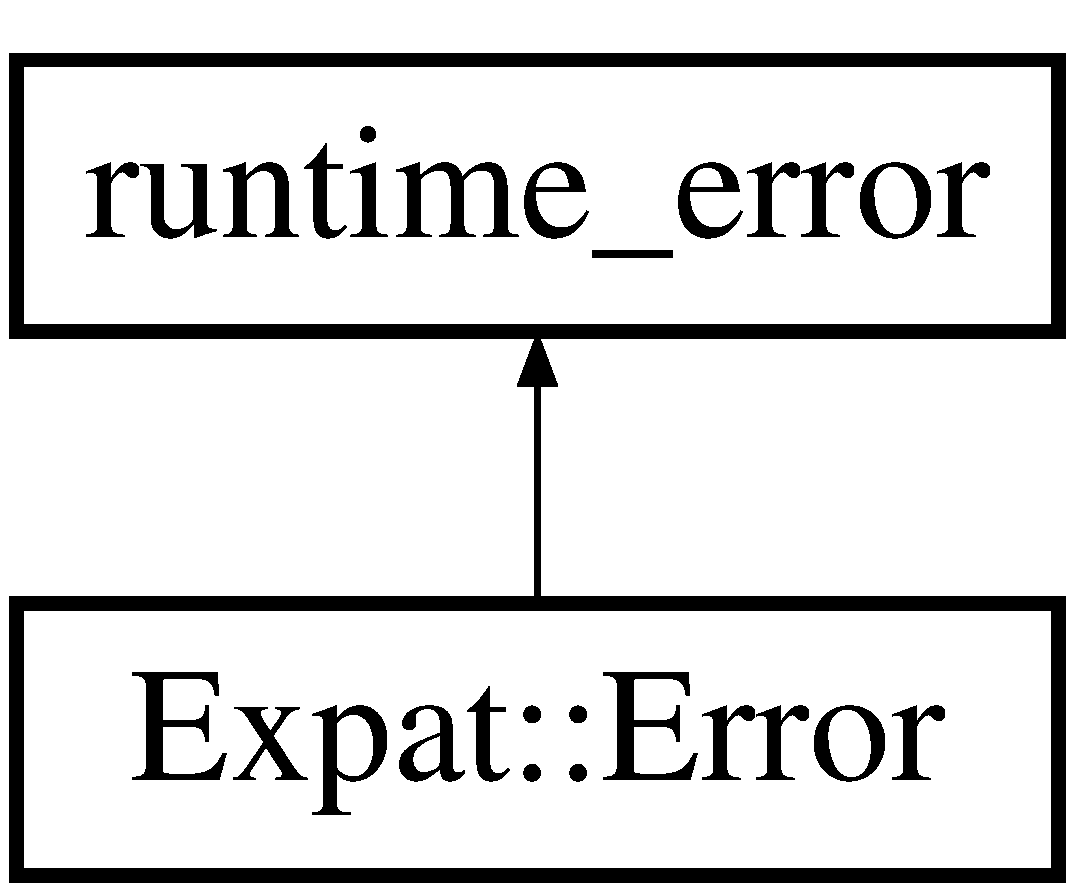
\includegraphics[height=2.000000cm]{class_expat_1_1_error}
\end{center}
\end{figure}
\subsection*{Public Member Functions}
\begin{DoxyCompactItemize}
\item 
\hyperlink{class_expat_1_1_error_acd92f134209cff2484b670af3be415ba}{Error} (X\+M\+L\+\_\+\+Error code)
\item 
\hyperlink{class_expat_1_1_error_a70a379a6a692a1f70929704cd43cb4cf}{Error} (const \hyperlink{class_expat_1_1_error}{Error} \&)=default
\item 
\hyperlink{class_expat_1_1_error_a194760fc6775aaadb65df818e7655330}{$\sim$\+Error} ()  throw ()
\item 
X\+M\+L\+\_\+\+Error \hyperlink{class_expat_1_1_error_a9a0d1a9ca664b60284c481ba094dac1e}{get\+Code} () const
\item 
\hyperlink{class_expat_1_1_error}{Error} \& \hyperlink{class_expat_1_1_error_ace2f59b903c510d0ac58613f3a2c6e4a}{operator=} (const \hyperlink{class_expat_1_1_error}{Error} \&)=default
\end{DoxyCompactItemize}
\subsection*{Protected Attributes}
\begin{DoxyCompactItemize}
\item 
X\+M\+L\+\_\+\+Error \hyperlink{class_expat_1_1_error_a6536d64df7df917a68f5984aaf2108a1}{m\+Code}
\end{DoxyCompactItemize}


\subsection{Constructor \& Destructor Documentation}
\hypertarget{class_expat_1_1_error_acd92f134209cff2484b670af3be415ba}{}\label{class_expat_1_1_error_acd92f134209cff2484b670af3be415ba} 
\index{Expat\+::\+Error@{Expat\+::\+Error}!Error@{Error}}
\index{Error@{Error}!Expat\+::\+Error@{Expat\+::\+Error}}
\subsubsection{\texorpdfstring{Error()}{Error()}\hspace{0.1cm}{\footnotesize\ttfamily [1/2]}}
{\footnotesize\ttfamily Expat\+::\+Error\+::\+Error (\begin{DoxyParamCaption}\item[{X\+M\+L\+\_\+\+Error}]{code }\end{DoxyParamCaption})}

\hypertarget{class_expat_1_1_error_a70a379a6a692a1f70929704cd43cb4cf}{}\label{class_expat_1_1_error_a70a379a6a692a1f70929704cd43cb4cf} 
\index{Expat\+::\+Error@{Expat\+::\+Error}!Error@{Error}}
\index{Error@{Error}!Expat\+::\+Error@{Expat\+::\+Error}}
\subsubsection{\texorpdfstring{Error()}{Error()}\hspace{0.1cm}{\footnotesize\ttfamily [2/2]}}
{\footnotesize\ttfamily Expat\+::\+Error\+::\+Error (\begin{DoxyParamCaption}\item[{const \hyperlink{class_expat_1_1_error}{Error} \&}]{ }\end{DoxyParamCaption})\hspace{0.3cm}{\ttfamily [default]}}

\hypertarget{class_expat_1_1_error_a194760fc6775aaadb65df818e7655330}{}\label{class_expat_1_1_error_a194760fc6775aaadb65df818e7655330} 
\index{Expat\+::\+Error@{Expat\+::\+Error}!````~Error@{$\sim$\+Error}}
\index{````~Error@{$\sim$\+Error}!Expat\+::\+Error@{Expat\+::\+Error}}
\subsubsection{\texorpdfstring{$\sim$\+Error()}{~Error()}}
{\footnotesize\ttfamily Expat\+::\+Error\+::$\sim$\+Error (\begin{DoxyParamCaption}{ }\end{DoxyParamCaption}) throw  ) \hspace{0.3cm}{\ttfamily [inline]}}



\subsection{Member Function Documentation}
\hypertarget{class_expat_1_1_error_a9a0d1a9ca664b60284c481ba094dac1e}{}\label{class_expat_1_1_error_a9a0d1a9ca664b60284c481ba094dac1e} 
\index{Expat\+::\+Error@{Expat\+::\+Error}!get\+Code@{get\+Code}}
\index{get\+Code@{get\+Code}!Expat\+::\+Error@{Expat\+::\+Error}}
\subsubsection{\texorpdfstring{get\+Code()}{getCode()}}
{\footnotesize\ttfamily X\+M\+L\+\_\+\+Error Expat\+::\+Error\+::get\+Code (\begin{DoxyParamCaption}{ }\end{DoxyParamCaption}) const\hspace{0.3cm}{\ttfamily [inline]}}

\hypertarget{class_expat_1_1_error_ace2f59b903c510d0ac58613f3a2c6e4a}{}\label{class_expat_1_1_error_ace2f59b903c510d0ac58613f3a2c6e4a} 
\index{Expat\+::\+Error@{Expat\+::\+Error}!operator=@{operator=}}
\index{operator=@{operator=}!Expat\+::\+Error@{Expat\+::\+Error}}
\subsubsection{\texorpdfstring{operator=()}{operator=()}}
{\footnotesize\ttfamily \hyperlink{class_expat_1_1_error}{Error}\& Expat\+::\+Error\+::operator= (\begin{DoxyParamCaption}\item[{const \hyperlink{class_expat_1_1_error}{Error} \&}]{ }\end{DoxyParamCaption})\hspace{0.3cm}{\ttfamily [default]}}



\subsection{Member Data Documentation}
\hypertarget{class_expat_1_1_error_a6536d64df7df917a68f5984aaf2108a1}{}\label{class_expat_1_1_error_a6536d64df7df917a68f5984aaf2108a1} 
\index{Expat\+::\+Error@{Expat\+::\+Error}!m\+Code@{m\+Code}}
\index{m\+Code@{m\+Code}!Expat\+::\+Error@{Expat\+::\+Error}}
\subsubsection{\texorpdfstring{m\+Code}{mCode}}
{\footnotesize\ttfamily X\+M\+L\+\_\+\+Error Expat\+::\+Error\+::m\+Code\hspace{0.3cm}{\ttfamily [protected]}}



The documentation for this class was generated from the following files\+:\begin{DoxyCompactItemize}
\item 
src/\hyperlink{expat_parse_8h}{expat\+Parse.\+h}\item 
src/\hyperlink{expatparse_8cpp}{expatparse.\+cpp}\end{DoxyCompactItemize}

\hypertarget{class_n_z_b_1_1_file}{}\section{N\+ZB\+:\+:File Class Reference}
\label{class_n_z_b_1_1_file}\index{N\+Z\+B\+::\+File@{N\+Z\+B\+::\+File}}


{\ttfamily \#include $<$nzb.\+h$>$}

\subsection*{Public Member Functions}
\begin{DoxyCompactItemize}
\item 
\hyperlink{class_n_z_b_1_1_file_ac5e08598cb3f05601149485eb02eae7a}{File} ()
\item 
\hyperlink{class_n_z_b_1_1_file_a1d87fa686b8f2cb0c2b8820ef088ba05}{File} (const char $\ast$subject, const char $\ast$poster, time\+\_\+t timestamp)
\item 
\hyperlink{class_n_z_b_1_1_file_af83c62781c50d7cc8e1808234920b8a6}{File} (int segment\+Count, \hyperlink{class_n_z_b_1_1_segment}{Segment} $\ast$p\+Segments, int group\+Count, \hyperlink{class_n_z_b_1_1_group}{Group} $\ast$p\+Groups)
\item 
\hyperlink{class_n_z_b_1_1_file_a3863e5112bd3e0ee5be4770bc7b4cb5e}{File} (\hyperlink{class_n_z_b_1_1_file}{File} \&\&rv\+File)
\item 
\hyperlink{class_n_z_b_1_1_file_ab9c267164945ff326166490b427b7393}{$\sim$\+File} ()
\item 
time\+\_\+t \hyperlink{class_n_z_b_1_1_file_a01adb6cd77a2f9546043aec2d8fef936}{get\+Timestamp} () const
\item 
std\+::string \& \hyperlink{class_n_z_b_1_1_file_a1110d411e6e7fd3ecb9b7f74e476924b}{get\+Subject} ()
\item 
const std\+::string \& \hyperlink{class_n_z_b_1_1_file_aa14b0404ce708a3cd15c7aa6803704ee}{get\+Subject} () const
\item 
std\+::string \& \hyperlink{class_n_z_b_1_1_file_a5203542d4807f92d520c6101a8927af9}{get\+Poster} ()
\item 
const std\+::string \& \hyperlink{class_n_z_b_1_1_file_af093b1edbffcafdae7f37c05d6581d0e}{get\+Poster} () const
\item 
int \hyperlink{class_n_z_b_1_1_file_a2aab94f806e5cc265413e3ad4d7e5ec2}{get\+Segment\+Count} () const
\item 
\hyperlink{class_n_z_b_1_1_segment}{Segment} \& \hyperlink{class_n_z_b_1_1_file_a5f4d723636e54b354f89c34cd3e578cb}{get\+Segment} (int i\+Segment)
\item 
const \hyperlink{class_n_z_b_1_1_segment}{Segment} \& \hyperlink{class_n_z_b_1_1_file_a092df4f0a0e79ebf21c033f45d83b67f}{get\+Segment} (int i\+Segment) const
\item 
void \hyperlink{class_n_z_b_1_1_file_a35796f99c09199259761c16295635349}{set\+Segments} (int count, \hyperlink{class_n_z_b_1_1_segment}{Segment} $\ast$p\+Segments)
\item 
int \hyperlink{class_n_z_b_1_1_file_a423866b094bc656afbb4cf6a3667c8b6}{get\+Group\+Count} () const
\item 
\hyperlink{class_n_z_b_1_1_group}{Group} \& \hyperlink{class_n_z_b_1_1_file_a7baaa4ddddfbe5a63671329cf239d8f5}{get\+Group} (int i\+Group)
\item 
const \hyperlink{class_n_z_b_1_1_group}{Group} \& \hyperlink{class_n_z_b_1_1_file_a286c4fc01910d1c1e9d70369d768b641}{get\+Group} (int i\+Group) const
\item 
void \hyperlink{class_n_z_b_1_1_file_a3316ed024ea100d7afefcc9f5bcba25f}{set\+Groups} (int count, \hyperlink{class_n_z_b_1_1_group}{Group} $\ast$p\+Groups)
\item 
\hyperlink{class_n_z_b_1_1_file}{File} \& \hyperlink{class_n_z_b_1_1_file_a29355ed8ab7a8bd97588b8a1ade358de}{operator=} (\hyperlink{class_n_z_b_1_1_file}{File} \&\&rv\+File)
\end{DoxyCompactItemize}
\subsection*{Protected Attributes}
\begin{DoxyCompactItemize}
\item 
time\+\_\+t \hyperlink{class_n_z_b_1_1_file_a57e957204ffcb538b70c98a9c000e6ab}{m\+Timestamp}
\item 
std\+::string \hyperlink{class_n_z_b_1_1_file_a426bdfb4be69a92a56afa2fe0d16e522}{m\+Subject}
\item 
std\+::string \hyperlink{class_n_z_b_1_1_file_ad50b2da39f242433c24ae28be16a2429}{m\+Poster}
\item 
int \hyperlink{class_n_z_b_1_1_file_a7b60730fb288ccc891a16256a935dbba}{m\+Segment\+Count}
\item 
\hyperlink{class_n_z_b_1_1_segment}{Segment} $\ast$ \hyperlink{class_n_z_b_1_1_file_ad8d7a8167b46230dd86439cb95a98cb7}{mp\+Segments}
\item 
int \hyperlink{class_n_z_b_1_1_file_aaf96258452951818ba93e90a5f0de6b6}{m\+Group\+Count}
\item 
\hyperlink{class_n_z_b_1_1_group}{Group} $\ast$ \hyperlink{class_n_z_b_1_1_file_a1afca4ebb4dd759001b70e64ae4c8136}{mp\+Groups}
\end{DoxyCompactItemize}


\subsection{Constructor \& Destructor Documentation}
\hypertarget{class_n_z_b_1_1_file_ac5e08598cb3f05601149485eb02eae7a}{}\label{class_n_z_b_1_1_file_ac5e08598cb3f05601149485eb02eae7a} 
\index{N\+Z\+B\+::\+File@{N\+Z\+B\+::\+File}!File@{File}}
\index{File@{File}!N\+Z\+B\+::\+File@{N\+Z\+B\+::\+File}}
\subsubsection{\texorpdfstring{File()}{File()}\hspace{0.1cm}{\footnotesize\ttfamily [1/4]}}
{\footnotesize\ttfamily N\+Z\+B\+::\+File\+::\+File (\begin{DoxyParamCaption}{ }\end{DoxyParamCaption})\hspace{0.3cm}{\ttfamily [inline]}}

\hypertarget{class_n_z_b_1_1_file_a1d87fa686b8f2cb0c2b8820ef088ba05}{}\label{class_n_z_b_1_1_file_a1d87fa686b8f2cb0c2b8820ef088ba05} 
\index{N\+Z\+B\+::\+File@{N\+Z\+B\+::\+File}!File@{File}}
\index{File@{File}!N\+Z\+B\+::\+File@{N\+Z\+B\+::\+File}}
\subsubsection{\texorpdfstring{File()}{File()}\hspace{0.1cm}{\footnotesize\ttfamily [2/4]}}
{\footnotesize\ttfamily N\+Z\+B\+::\+File\+::\+File (\begin{DoxyParamCaption}\item[{const char $\ast$}]{subject,  }\item[{const char $\ast$}]{poster,  }\item[{time\+\_\+t}]{timestamp }\end{DoxyParamCaption})}

\hypertarget{class_n_z_b_1_1_file_af83c62781c50d7cc8e1808234920b8a6}{}\label{class_n_z_b_1_1_file_af83c62781c50d7cc8e1808234920b8a6} 
\index{N\+Z\+B\+::\+File@{N\+Z\+B\+::\+File}!File@{File}}
\index{File@{File}!N\+Z\+B\+::\+File@{N\+Z\+B\+::\+File}}
\subsubsection{\texorpdfstring{File()}{File()}\hspace{0.1cm}{\footnotesize\ttfamily [3/4]}}
{\footnotesize\ttfamily N\+Z\+B\+::\+File\+::\+File (\begin{DoxyParamCaption}\item[{int}]{segment\+Count,  }\item[{\hyperlink{class_n_z_b_1_1_segment}{Segment} $\ast$}]{p\+Segments,  }\item[{int}]{group\+Count,  }\item[{\hyperlink{class_n_z_b_1_1_group}{Group} $\ast$}]{p\+Groups }\end{DoxyParamCaption})}

\hypertarget{class_n_z_b_1_1_file_a3863e5112bd3e0ee5be4770bc7b4cb5e}{}\label{class_n_z_b_1_1_file_a3863e5112bd3e0ee5be4770bc7b4cb5e} 
\index{N\+Z\+B\+::\+File@{N\+Z\+B\+::\+File}!File@{File}}
\index{File@{File}!N\+Z\+B\+::\+File@{N\+Z\+B\+::\+File}}
\subsubsection{\texorpdfstring{File()}{File()}\hspace{0.1cm}{\footnotesize\ttfamily [4/4]}}
{\footnotesize\ttfamily N\+Z\+B\+::\+File\+::\+File (\begin{DoxyParamCaption}\item[{\hyperlink{class_n_z_b_1_1_file}{File} \&\&}]{rv\+File }\end{DoxyParamCaption})}

\hypertarget{class_n_z_b_1_1_file_ab9c267164945ff326166490b427b7393}{}\label{class_n_z_b_1_1_file_ab9c267164945ff326166490b427b7393} 
\index{N\+Z\+B\+::\+File@{N\+Z\+B\+::\+File}!````~File@{$\sim$\+File}}
\index{````~File@{$\sim$\+File}!N\+Z\+B\+::\+File@{N\+Z\+B\+::\+File}}
\subsubsection{\texorpdfstring{$\sim$\+File()}{~File()}}
{\footnotesize\ttfamily N\+Z\+B\+::\+File\+::$\sim$\+File (\begin{DoxyParamCaption}{ }\end{DoxyParamCaption})}



\subsection{Member Function Documentation}
\hypertarget{class_n_z_b_1_1_file_a7baaa4ddddfbe5a63671329cf239d8f5}{}\label{class_n_z_b_1_1_file_a7baaa4ddddfbe5a63671329cf239d8f5} 
\index{N\+Z\+B\+::\+File@{N\+Z\+B\+::\+File}!get\+Group@{get\+Group}}
\index{get\+Group@{get\+Group}!N\+Z\+B\+::\+File@{N\+Z\+B\+::\+File}}
\subsubsection{\texorpdfstring{get\+Group()}{getGroup()}\hspace{0.1cm}{\footnotesize\ttfamily [1/2]}}
{\footnotesize\ttfamily \hyperlink{class_n_z_b_1_1_group}{Group} \& N\+Z\+B\+::\+File\+::get\+Group (\begin{DoxyParamCaption}\item[{int}]{i\+Group }\end{DoxyParamCaption})}

\hypertarget{class_n_z_b_1_1_file_a286c4fc01910d1c1e9d70369d768b641}{}\label{class_n_z_b_1_1_file_a286c4fc01910d1c1e9d70369d768b641} 
\index{N\+Z\+B\+::\+File@{N\+Z\+B\+::\+File}!get\+Group@{get\+Group}}
\index{get\+Group@{get\+Group}!N\+Z\+B\+::\+File@{N\+Z\+B\+::\+File}}
\subsubsection{\texorpdfstring{get\+Group()}{getGroup()}\hspace{0.1cm}{\footnotesize\ttfamily [2/2]}}
{\footnotesize\ttfamily const \hyperlink{class_n_z_b_1_1_group}{Group} \& N\+Z\+B\+::\+File\+::get\+Group (\begin{DoxyParamCaption}\item[{int}]{i\+Group }\end{DoxyParamCaption}) const}

\hypertarget{class_n_z_b_1_1_file_a423866b094bc656afbb4cf6a3667c8b6}{}\label{class_n_z_b_1_1_file_a423866b094bc656afbb4cf6a3667c8b6} 
\index{N\+Z\+B\+::\+File@{N\+Z\+B\+::\+File}!get\+Group\+Count@{get\+Group\+Count}}
\index{get\+Group\+Count@{get\+Group\+Count}!N\+Z\+B\+::\+File@{N\+Z\+B\+::\+File}}
\subsubsection{\texorpdfstring{get\+Group\+Count()}{getGroupCount()}}
{\footnotesize\ttfamily int N\+Z\+B\+::\+File\+::get\+Group\+Count (\begin{DoxyParamCaption}{ }\end{DoxyParamCaption}) const\hspace{0.3cm}{\ttfamily [inline]}}

\hypertarget{class_n_z_b_1_1_file_a5203542d4807f92d520c6101a8927af9}{}\label{class_n_z_b_1_1_file_a5203542d4807f92d520c6101a8927af9} 
\index{N\+Z\+B\+::\+File@{N\+Z\+B\+::\+File}!get\+Poster@{get\+Poster}}
\index{get\+Poster@{get\+Poster}!N\+Z\+B\+::\+File@{N\+Z\+B\+::\+File}}
\subsubsection{\texorpdfstring{get\+Poster()}{getPoster()}\hspace{0.1cm}{\footnotesize\ttfamily [1/2]}}
{\footnotesize\ttfamily std\+::string\& N\+Z\+B\+::\+File\+::get\+Poster (\begin{DoxyParamCaption}{ }\end{DoxyParamCaption})\hspace{0.3cm}{\ttfamily [inline]}}

\hypertarget{class_n_z_b_1_1_file_af093b1edbffcafdae7f37c05d6581d0e}{}\label{class_n_z_b_1_1_file_af093b1edbffcafdae7f37c05d6581d0e} 
\index{N\+Z\+B\+::\+File@{N\+Z\+B\+::\+File}!get\+Poster@{get\+Poster}}
\index{get\+Poster@{get\+Poster}!N\+Z\+B\+::\+File@{N\+Z\+B\+::\+File}}
\subsubsection{\texorpdfstring{get\+Poster()}{getPoster()}\hspace{0.1cm}{\footnotesize\ttfamily [2/2]}}
{\footnotesize\ttfamily const std\+::string\& N\+Z\+B\+::\+File\+::get\+Poster (\begin{DoxyParamCaption}{ }\end{DoxyParamCaption}) const\hspace{0.3cm}{\ttfamily [inline]}}

\hypertarget{class_n_z_b_1_1_file_a5f4d723636e54b354f89c34cd3e578cb}{}\label{class_n_z_b_1_1_file_a5f4d723636e54b354f89c34cd3e578cb} 
\index{N\+Z\+B\+::\+File@{N\+Z\+B\+::\+File}!get\+Segment@{get\+Segment}}
\index{get\+Segment@{get\+Segment}!N\+Z\+B\+::\+File@{N\+Z\+B\+::\+File}}
\subsubsection{\texorpdfstring{get\+Segment()}{getSegment()}\hspace{0.1cm}{\footnotesize\ttfamily [1/2]}}
{\footnotesize\ttfamily \hyperlink{class_n_z_b_1_1_segment}{Segment} \& N\+Z\+B\+::\+File\+::get\+Segment (\begin{DoxyParamCaption}\item[{int}]{i\+Segment }\end{DoxyParamCaption})}

\hypertarget{class_n_z_b_1_1_file_a092df4f0a0e79ebf21c033f45d83b67f}{}\label{class_n_z_b_1_1_file_a092df4f0a0e79ebf21c033f45d83b67f} 
\index{N\+Z\+B\+::\+File@{N\+Z\+B\+::\+File}!get\+Segment@{get\+Segment}}
\index{get\+Segment@{get\+Segment}!N\+Z\+B\+::\+File@{N\+Z\+B\+::\+File}}
\subsubsection{\texorpdfstring{get\+Segment()}{getSegment()}\hspace{0.1cm}{\footnotesize\ttfamily [2/2]}}
{\footnotesize\ttfamily const \hyperlink{class_n_z_b_1_1_segment}{Segment} \& N\+Z\+B\+::\+File\+::get\+Segment (\begin{DoxyParamCaption}\item[{int}]{i\+Segment }\end{DoxyParamCaption}) const}

\hypertarget{class_n_z_b_1_1_file_a2aab94f806e5cc265413e3ad4d7e5ec2}{}\label{class_n_z_b_1_1_file_a2aab94f806e5cc265413e3ad4d7e5ec2} 
\index{N\+Z\+B\+::\+File@{N\+Z\+B\+::\+File}!get\+Segment\+Count@{get\+Segment\+Count}}
\index{get\+Segment\+Count@{get\+Segment\+Count}!N\+Z\+B\+::\+File@{N\+Z\+B\+::\+File}}
\subsubsection{\texorpdfstring{get\+Segment\+Count()}{getSegmentCount()}}
{\footnotesize\ttfamily int N\+Z\+B\+::\+File\+::get\+Segment\+Count (\begin{DoxyParamCaption}{ }\end{DoxyParamCaption}) const\hspace{0.3cm}{\ttfamily [inline]}}

\hypertarget{class_n_z_b_1_1_file_a1110d411e6e7fd3ecb9b7f74e476924b}{}\label{class_n_z_b_1_1_file_a1110d411e6e7fd3ecb9b7f74e476924b} 
\index{N\+Z\+B\+::\+File@{N\+Z\+B\+::\+File}!get\+Subject@{get\+Subject}}
\index{get\+Subject@{get\+Subject}!N\+Z\+B\+::\+File@{N\+Z\+B\+::\+File}}
\subsubsection{\texorpdfstring{get\+Subject()}{getSubject()}\hspace{0.1cm}{\footnotesize\ttfamily [1/2]}}
{\footnotesize\ttfamily std\+::string\& N\+Z\+B\+::\+File\+::get\+Subject (\begin{DoxyParamCaption}{ }\end{DoxyParamCaption})\hspace{0.3cm}{\ttfamily [inline]}}

\hypertarget{class_n_z_b_1_1_file_aa14b0404ce708a3cd15c7aa6803704ee}{}\label{class_n_z_b_1_1_file_aa14b0404ce708a3cd15c7aa6803704ee} 
\index{N\+Z\+B\+::\+File@{N\+Z\+B\+::\+File}!get\+Subject@{get\+Subject}}
\index{get\+Subject@{get\+Subject}!N\+Z\+B\+::\+File@{N\+Z\+B\+::\+File}}
\subsubsection{\texorpdfstring{get\+Subject()}{getSubject()}\hspace{0.1cm}{\footnotesize\ttfamily [2/2]}}
{\footnotesize\ttfamily const std\+::string\& N\+Z\+B\+::\+File\+::get\+Subject (\begin{DoxyParamCaption}{ }\end{DoxyParamCaption}) const\hspace{0.3cm}{\ttfamily [inline]}}

\hypertarget{class_n_z_b_1_1_file_a01adb6cd77a2f9546043aec2d8fef936}{}\label{class_n_z_b_1_1_file_a01adb6cd77a2f9546043aec2d8fef936} 
\index{N\+Z\+B\+::\+File@{N\+Z\+B\+::\+File}!get\+Timestamp@{get\+Timestamp}}
\index{get\+Timestamp@{get\+Timestamp}!N\+Z\+B\+::\+File@{N\+Z\+B\+::\+File}}
\subsubsection{\texorpdfstring{get\+Timestamp()}{getTimestamp()}}
{\footnotesize\ttfamily time\+\_\+t N\+Z\+B\+::\+File\+::get\+Timestamp (\begin{DoxyParamCaption}{ }\end{DoxyParamCaption}) const\hspace{0.3cm}{\ttfamily [inline]}}

\hypertarget{class_n_z_b_1_1_file_a29355ed8ab7a8bd97588b8a1ade358de}{}\label{class_n_z_b_1_1_file_a29355ed8ab7a8bd97588b8a1ade358de} 
\index{N\+Z\+B\+::\+File@{N\+Z\+B\+::\+File}!operator=@{operator=}}
\index{operator=@{operator=}!N\+Z\+B\+::\+File@{N\+Z\+B\+::\+File}}
\subsubsection{\texorpdfstring{operator=()}{operator=()}}
{\footnotesize\ttfamily \hyperlink{class_n_z_b_1_1_file}{File} \& N\+Z\+B\+::\+File\+::operator= (\begin{DoxyParamCaption}\item[{\hyperlink{class_n_z_b_1_1_file}{File} \&\&}]{rv\+File }\end{DoxyParamCaption})}

\hypertarget{class_n_z_b_1_1_file_a3316ed024ea100d7afefcc9f5bcba25f}{}\label{class_n_z_b_1_1_file_a3316ed024ea100d7afefcc9f5bcba25f} 
\index{N\+Z\+B\+::\+File@{N\+Z\+B\+::\+File}!set\+Groups@{set\+Groups}}
\index{set\+Groups@{set\+Groups}!N\+Z\+B\+::\+File@{N\+Z\+B\+::\+File}}
\subsubsection{\texorpdfstring{set\+Groups()}{setGroups()}}
{\footnotesize\ttfamily void N\+Z\+B\+::\+File\+::set\+Groups (\begin{DoxyParamCaption}\item[{int}]{count,  }\item[{\hyperlink{class_n_z_b_1_1_group}{Group} $\ast$}]{p\+Groups }\end{DoxyParamCaption})}

\hypertarget{class_n_z_b_1_1_file_a35796f99c09199259761c16295635349}{}\label{class_n_z_b_1_1_file_a35796f99c09199259761c16295635349} 
\index{N\+Z\+B\+::\+File@{N\+Z\+B\+::\+File}!set\+Segments@{set\+Segments}}
\index{set\+Segments@{set\+Segments}!N\+Z\+B\+::\+File@{N\+Z\+B\+::\+File}}
\subsubsection{\texorpdfstring{set\+Segments()}{setSegments()}}
{\footnotesize\ttfamily void N\+Z\+B\+::\+File\+::set\+Segments (\begin{DoxyParamCaption}\item[{int}]{count,  }\item[{\hyperlink{class_n_z_b_1_1_segment}{Segment} $\ast$}]{p\+Segments }\end{DoxyParamCaption})}



\subsection{Member Data Documentation}
\hypertarget{class_n_z_b_1_1_file_aaf96258452951818ba93e90a5f0de6b6}{}\label{class_n_z_b_1_1_file_aaf96258452951818ba93e90a5f0de6b6} 
\index{N\+Z\+B\+::\+File@{N\+Z\+B\+::\+File}!m\+Group\+Count@{m\+Group\+Count}}
\index{m\+Group\+Count@{m\+Group\+Count}!N\+Z\+B\+::\+File@{N\+Z\+B\+::\+File}}
\subsubsection{\texorpdfstring{m\+Group\+Count}{mGroupCount}}
{\footnotesize\ttfamily int N\+Z\+B\+::\+File\+::m\+Group\+Count\hspace{0.3cm}{\ttfamily [protected]}}

\hypertarget{class_n_z_b_1_1_file_a1afca4ebb4dd759001b70e64ae4c8136}{}\label{class_n_z_b_1_1_file_a1afca4ebb4dd759001b70e64ae4c8136} 
\index{N\+Z\+B\+::\+File@{N\+Z\+B\+::\+File}!mp\+Groups@{mp\+Groups}}
\index{mp\+Groups@{mp\+Groups}!N\+Z\+B\+::\+File@{N\+Z\+B\+::\+File}}
\subsubsection{\texorpdfstring{mp\+Groups}{mpGroups}}
{\footnotesize\ttfamily \hyperlink{class_n_z_b_1_1_group}{Group}$\ast$ N\+Z\+B\+::\+File\+::mp\+Groups\hspace{0.3cm}{\ttfamily [protected]}}

\hypertarget{class_n_z_b_1_1_file_ad50b2da39f242433c24ae28be16a2429}{}\label{class_n_z_b_1_1_file_ad50b2da39f242433c24ae28be16a2429} 
\index{N\+Z\+B\+::\+File@{N\+Z\+B\+::\+File}!m\+Poster@{m\+Poster}}
\index{m\+Poster@{m\+Poster}!N\+Z\+B\+::\+File@{N\+Z\+B\+::\+File}}
\subsubsection{\texorpdfstring{m\+Poster}{mPoster}}
{\footnotesize\ttfamily std\+::string N\+Z\+B\+::\+File\+::m\+Poster\hspace{0.3cm}{\ttfamily [protected]}}

\hypertarget{class_n_z_b_1_1_file_ad8d7a8167b46230dd86439cb95a98cb7}{}\label{class_n_z_b_1_1_file_ad8d7a8167b46230dd86439cb95a98cb7} 
\index{N\+Z\+B\+::\+File@{N\+Z\+B\+::\+File}!mp\+Segments@{mp\+Segments}}
\index{mp\+Segments@{mp\+Segments}!N\+Z\+B\+::\+File@{N\+Z\+B\+::\+File}}
\subsubsection{\texorpdfstring{mp\+Segments}{mpSegments}}
{\footnotesize\ttfamily \hyperlink{class_n_z_b_1_1_segment}{Segment}$\ast$ N\+Z\+B\+::\+File\+::mp\+Segments\hspace{0.3cm}{\ttfamily [protected]}}

\hypertarget{class_n_z_b_1_1_file_a7b60730fb288ccc891a16256a935dbba}{}\label{class_n_z_b_1_1_file_a7b60730fb288ccc891a16256a935dbba} 
\index{N\+Z\+B\+::\+File@{N\+Z\+B\+::\+File}!m\+Segment\+Count@{m\+Segment\+Count}}
\index{m\+Segment\+Count@{m\+Segment\+Count}!N\+Z\+B\+::\+File@{N\+Z\+B\+::\+File}}
\subsubsection{\texorpdfstring{m\+Segment\+Count}{mSegmentCount}}
{\footnotesize\ttfamily int N\+Z\+B\+::\+File\+::m\+Segment\+Count\hspace{0.3cm}{\ttfamily [protected]}}

\hypertarget{class_n_z_b_1_1_file_a426bdfb4be69a92a56afa2fe0d16e522}{}\label{class_n_z_b_1_1_file_a426bdfb4be69a92a56afa2fe0d16e522} 
\index{N\+Z\+B\+::\+File@{N\+Z\+B\+::\+File}!m\+Subject@{m\+Subject}}
\index{m\+Subject@{m\+Subject}!N\+Z\+B\+::\+File@{N\+Z\+B\+::\+File}}
\subsubsection{\texorpdfstring{m\+Subject}{mSubject}}
{\footnotesize\ttfamily std\+::string N\+Z\+B\+::\+File\+::m\+Subject\hspace{0.3cm}{\ttfamily [protected]}}

\hypertarget{class_n_z_b_1_1_file_a57e957204ffcb538b70c98a9c000e6ab}{}\label{class_n_z_b_1_1_file_a57e957204ffcb538b70c98a9c000e6ab} 
\index{N\+Z\+B\+::\+File@{N\+Z\+B\+::\+File}!m\+Timestamp@{m\+Timestamp}}
\index{m\+Timestamp@{m\+Timestamp}!N\+Z\+B\+::\+File@{N\+Z\+B\+::\+File}}
\subsubsection{\texorpdfstring{m\+Timestamp}{mTimestamp}}
{\footnotesize\ttfamily time\+\_\+t N\+Z\+B\+::\+File\+::m\+Timestamp\hspace{0.3cm}{\ttfamily [protected]}}



The documentation for this class was generated from the following files\+:\begin{DoxyCompactItemize}
\item 
src/include/libusenet/\hyperlink{nzb_8h}{nzb.\+h}\item 
src/\hyperlink{nzb_8cpp}{nzb.\+cpp}\end{DoxyCompactItemize}

\hypertarget{class_n_z_b_1_1_file_collection}{}\section{N\+ZB\+:\+:File\+Collection Class Reference}
\label{class_n_z_b_1_1_file_collection}\index{N\+Z\+B\+::\+File\+Collection@{N\+Z\+B\+::\+File\+Collection}}


{\ttfamily \#include $<$nzb.\+h$>$}

\subsection*{Public Member Functions}
\begin{DoxyCompactItemize}
\item 
\hyperlink{class_n_z_b_1_1_file_collection_a2ae200e24e6a4ee4d1be8e649f72aba9}{File\+Collection} ()
\item 
\hyperlink{class_n_z_b_1_1_file_collection_a76662806b20ecb79fb1c4800df2ee9df}{File\+Collection} (int file\+Count, int segment\+Count, int group\+Count)
\item 
\hyperlink{class_n_z_b_1_1_file_collection_ab14971382a51c26233307404bacfa8e6}{File\+Collection} (\hyperlink{class_n_z_b_1_1_file_collection}{File\+Collection} \&\&rv\+Collection)
\item 
\hyperlink{class_n_z_b_1_1_file_collection_a1eeded48503a89ccc75e7446df3f7e3f}{File\+Collection} (const \hyperlink{class_n_z_b_1_1_file_collection}{File\+Collection} \&)=delete
\item 
\hyperlink{class_n_z_b_1_1_file_collection_a6d6986c488c8124efea37ef187589b88}{$\sim$\+File\+Collection} ()
\item 
int \hyperlink{class_n_z_b_1_1_file_collection_a33c0008fc18310d0a89fd72c38586c9a}{get\+File\+Count} () const
\item 
\hyperlink{class_n_z_b_1_1_file}{File} $\ast$ \hyperlink{class_n_z_b_1_1_file_collection_a921a80a0f09e9bd067566e236e5c688a}{get\+Files} ()
\item 
const \hyperlink{class_n_z_b_1_1_file}{File} $\ast$ \hyperlink{class_n_z_b_1_1_file_collection_a8b13dca0410b84a05aaeabe7e819b8cd}{get\+Files} () const
\item 
\hyperlink{class_n_z_b_1_1_file}{File} \& \hyperlink{class_n_z_b_1_1_file_collection_a60d75d8e870b9360ff0f03596ffd3885}{operator\mbox{[}$\,$\mbox{]}} (int i\+File)
\item 
const \hyperlink{class_n_z_b_1_1_file}{File} \& \hyperlink{class_n_z_b_1_1_file_collection_a169b09f36849f6e0c842939ae61cc383}{operator\mbox{[}$\,$\mbox{]}} (int i\+File) const
\item 
\hyperlink{class_n_z_b_1_1_file}{File} $\ast$ \hyperlink{class_n_z_b_1_1_file_collection_a26b50aedb8d73b4fba8aef7792c9f699}{begin} ()
\item 
\hyperlink{class_n_z_b_1_1_file}{File} $\ast$ \hyperlink{class_n_z_b_1_1_file_collection_ad792a3e63dad005cb44f6aa89a836673}{end} ()
\item 
const \hyperlink{class_n_z_b_1_1_file}{File} $\ast$ \hyperlink{class_n_z_b_1_1_file_collection_a9f357afe639a9fd066539466b9ce5d47}{begin} () const
\item 
const \hyperlink{class_n_z_b_1_1_file}{File} $\ast$ \hyperlink{class_n_z_b_1_1_file_collection_a781f4a5fec907bc7e46e144a300dd174}{end} () const
\item 
void \hyperlink{class_n_z_b_1_1_file_collection_a4caeac68cec4f2bd02fe82255ba52d33}{alloc} (int file\+Count, int segment\+Count, int group\+Count)
\item 
void \hyperlink{class_n_z_b_1_1_file_collection_a8888183a256a7afbbbdde5b19f2fbf9f}{free} ()
\item 
\hyperlink{class_n_z_b_1_1_file_collection}{File\+Collection} \& \hyperlink{class_n_z_b_1_1_file_collection_a974ea8d9e7851511eddf7c6bbb82741f}{operator=} (\hyperlink{class_n_z_b_1_1_file_collection}{File\+Collection} \&\&rv\+Collection)
\item 
\hyperlink{class_n_z_b_1_1_file_collection}{File\+Collection} \& \hyperlink{class_n_z_b_1_1_file_collection_a9a39412f971ae08850615fd4eaca730a}{operator=} (const \hyperlink{class_n_z_b_1_1_file_collection}{File\+Collection} \&)=delete
\end{DoxyCompactItemize}
\subsection*{Protected Attributes}
\begin{DoxyCompactItemize}
\item 
std\+::unique\+\_\+ptr$<$ unsigned char\mbox{[}$\,$\mbox{]}$>$ \hyperlink{class_n_z_b_1_1_file_collection_aee454b60ab12185c5328e950d5b1d444}{mp\+Mem}
\item 
int \hyperlink{class_n_z_b_1_1_file_collection_a54a530b2c5e4e487d588eee98e403cbe}{m\+File\+Count}
\end{DoxyCompactItemize}


\subsection{Constructor \& Destructor Documentation}
\hypertarget{class_n_z_b_1_1_file_collection_a2ae200e24e6a4ee4d1be8e649f72aba9}{}\label{class_n_z_b_1_1_file_collection_a2ae200e24e6a4ee4d1be8e649f72aba9} 
\index{N\+Z\+B\+::\+File\+Collection@{N\+Z\+B\+::\+File\+Collection}!File\+Collection@{File\+Collection}}
\index{File\+Collection@{File\+Collection}!N\+Z\+B\+::\+File\+Collection@{N\+Z\+B\+::\+File\+Collection}}
\subsubsection{\texorpdfstring{File\+Collection()}{FileCollection()}\hspace{0.1cm}{\footnotesize\ttfamily [1/4]}}
{\footnotesize\ttfamily N\+Z\+B\+::\+File\+Collection\+::\+File\+Collection (\begin{DoxyParamCaption}{ }\end{DoxyParamCaption})\hspace{0.3cm}{\ttfamily [inline]}}

\hypertarget{class_n_z_b_1_1_file_collection_a76662806b20ecb79fb1c4800df2ee9df}{}\label{class_n_z_b_1_1_file_collection_a76662806b20ecb79fb1c4800df2ee9df} 
\index{N\+Z\+B\+::\+File\+Collection@{N\+Z\+B\+::\+File\+Collection}!File\+Collection@{File\+Collection}}
\index{File\+Collection@{File\+Collection}!N\+Z\+B\+::\+File\+Collection@{N\+Z\+B\+::\+File\+Collection}}
\subsubsection{\texorpdfstring{File\+Collection()}{FileCollection()}\hspace{0.1cm}{\footnotesize\ttfamily [2/4]}}
{\footnotesize\ttfamily N\+Z\+B\+::\+File\+Collection\+::\+File\+Collection (\begin{DoxyParamCaption}\item[{int}]{file\+Count,  }\item[{int}]{segment\+Count,  }\item[{int}]{group\+Count }\end{DoxyParamCaption})}

\hypertarget{class_n_z_b_1_1_file_collection_ab14971382a51c26233307404bacfa8e6}{}\label{class_n_z_b_1_1_file_collection_ab14971382a51c26233307404bacfa8e6} 
\index{N\+Z\+B\+::\+File\+Collection@{N\+Z\+B\+::\+File\+Collection}!File\+Collection@{File\+Collection}}
\index{File\+Collection@{File\+Collection}!N\+Z\+B\+::\+File\+Collection@{N\+Z\+B\+::\+File\+Collection}}
\subsubsection{\texorpdfstring{File\+Collection()}{FileCollection()}\hspace{0.1cm}{\footnotesize\ttfamily [3/4]}}
{\footnotesize\ttfamily N\+Z\+B\+::\+File\+Collection\+::\+File\+Collection (\begin{DoxyParamCaption}\item[{\hyperlink{class_n_z_b_1_1_file_collection}{File\+Collection} \&\&}]{rv\+Collection }\end{DoxyParamCaption})}

\hypertarget{class_n_z_b_1_1_file_collection_a1eeded48503a89ccc75e7446df3f7e3f}{}\label{class_n_z_b_1_1_file_collection_a1eeded48503a89ccc75e7446df3f7e3f} 
\index{N\+Z\+B\+::\+File\+Collection@{N\+Z\+B\+::\+File\+Collection}!File\+Collection@{File\+Collection}}
\index{File\+Collection@{File\+Collection}!N\+Z\+B\+::\+File\+Collection@{N\+Z\+B\+::\+File\+Collection}}
\subsubsection{\texorpdfstring{File\+Collection()}{FileCollection()}\hspace{0.1cm}{\footnotesize\ttfamily [4/4]}}
{\footnotesize\ttfamily N\+Z\+B\+::\+File\+Collection\+::\+File\+Collection (\begin{DoxyParamCaption}\item[{const \hyperlink{class_n_z_b_1_1_file_collection}{File\+Collection} \&}]{ }\end{DoxyParamCaption})\hspace{0.3cm}{\ttfamily [delete]}}

\hypertarget{class_n_z_b_1_1_file_collection_a6d6986c488c8124efea37ef187589b88}{}\label{class_n_z_b_1_1_file_collection_a6d6986c488c8124efea37ef187589b88} 
\index{N\+Z\+B\+::\+File\+Collection@{N\+Z\+B\+::\+File\+Collection}!````~File\+Collection@{$\sim$\+File\+Collection}}
\index{````~File\+Collection@{$\sim$\+File\+Collection}!N\+Z\+B\+::\+File\+Collection@{N\+Z\+B\+::\+File\+Collection}}
\subsubsection{\texorpdfstring{$\sim$\+File\+Collection()}{~FileCollection()}}
{\footnotesize\ttfamily N\+Z\+B\+::\+File\+Collection\+::$\sim$\+File\+Collection (\begin{DoxyParamCaption}{ }\end{DoxyParamCaption})}



\subsection{Member Function Documentation}
\hypertarget{class_n_z_b_1_1_file_collection_a4caeac68cec4f2bd02fe82255ba52d33}{}\label{class_n_z_b_1_1_file_collection_a4caeac68cec4f2bd02fe82255ba52d33} 
\index{N\+Z\+B\+::\+File\+Collection@{N\+Z\+B\+::\+File\+Collection}!alloc@{alloc}}
\index{alloc@{alloc}!N\+Z\+B\+::\+File\+Collection@{N\+Z\+B\+::\+File\+Collection}}
\subsubsection{\texorpdfstring{alloc()}{alloc()}}
{\footnotesize\ttfamily void N\+Z\+B\+::\+File\+Collection\+::alloc (\begin{DoxyParamCaption}\item[{int}]{file\+Count,  }\item[{int}]{segment\+Count,  }\item[{int}]{group\+Count }\end{DoxyParamCaption})}

\hypertarget{class_n_z_b_1_1_file_collection_a26b50aedb8d73b4fba8aef7792c9f699}{}\label{class_n_z_b_1_1_file_collection_a26b50aedb8d73b4fba8aef7792c9f699} 
\index{N\+Z\+B\+::\+File\+Collection@{N\+Z\+B\+::\+File\+Collection}!begin@{begin}}
\index{begin@{begin}!N\+Z\+B\+::\+File\+Collection@{N\+Z\+B\+::\+File\+Collection}}
\subsubsection{\texorpdfstring{begin()}{begin()}\hspace{0.1cm}{\footnotesize\ttfamily [1/2]}}
{\footnotesize\ttfamily \hyperlink{class_n_z_b_1_1_file}{File} $\ast$ N\+Z\+B\+::\+File\+Collection\+::begin (\begin{DoxyParamCaption}{ }\end{DoxyParamCaption})}

\hypertarget{class_n_z_b_1_1_file_collection_a9f357afe639a9fd066539466b9ce5d47}{}\label{class_n_z_b_1_1_file_collection_a9f357afe639a9fd066539466b9ce5d47} 
\index{N\+Z\+B\+::\+File\+Collection@{N\+Z\+B\+::\+File\+Collection}!begin@{begin}}
\index{begin@{begin}!N\+Z\+B\+::\+File\+Collection@{N\+Z\+B\+::\+File\+Collection}}
\subsubsection{\texorpdfstring{begin()}{begin()}\hspace{0.1cm}{\footnotesize\ttfamily [2/2]}}
{\footnotesize\ttfamily const \hyperlink{class_n_z_b_1_1_file}{File} $\ast$ N\+Z\+B\+::\+File\+Collection\+::begin (\begin{DoxyParamCaption}{ }\end{DoxyParamCaption}) const}

\hypertarget{class_n_z_b_1_1_file_collection_ad792a3e63dad005cb44f6aa89a836673}{}\label{class_n_z_b_1_1_file_collection_ad792a3e63dad005cb44f6aa89a836673} 
\index{N\+Z\+B\+::\+File\+Collection@{N\+Z\+B\+::\+File\+Collection}!end@{end}}
\index{end@{end}!N\+Z\+B\+::\+File\+Collection@{N\+Z\+B\+::\+File\+Collection}}
\subsubsection{\texorpdfstring{end()}{end()}\hspace{0.1cm}{\footnotesize\ttfamily [1/2]}}
{\footnotesize\ttfamily \hyperlink{class_n_z_b_1_1_file}{File} $\ast$ N\+Z\+B\+::\+File\+Collection\+::end (\begin{DoxyParamCaption}{ }\end{DoxyParamCaption})}

\hypertarget{class_n_z_b_1_1_file_collection_a781f4a5fec907bc7e46e144a300dd174}{}\label{class_n_z_b_1_1_file_collection_a781f4a5fec907bc7e46e144a300dd174} 
\index{N\+Z\+B\+::\+File\+Collection@{N\+Z\+B\+::\+File\+Collection}!end@{end}}
\index{end@{end}!N\+Z\+B\+::\+File\+Collection@{N\+Z\+B\+::\+File\+Collection}}
\subsubsection{\texorpdfstring{end()}{end()}\hspace{0.1cm}{\footnotesize\ttfamily [2/2]}}
{\footnotesize\ttfamily const \hyperlink{class_n_z_b_1_1_file}{File} $\ast$ N\+Z\+B\+::\+File\+Collection\+::end (\begin{DoxyParamCaption}{ }\end{DoxyParamCaption}) const}

\hypertarget{class_n_z_b_1_1_file_collection_a8888183a256a7afbbbdde5b19f2fbf9f}{}\label{class_n_z_b_1_1_file_collection_a8888183a256a7afbbbdde5b19f2fbf9f} 
\index{N\+Z\+B\+::\+File\+Collection@{N\+Z\+B\+::\+File\+Collection}!free@{free}}
\index{free@{free}!N\+Z\+B\+::\+File\+Collection@{N\+Z\+B\+::\+File\+Collection}}
\subsubsection{\texorpdfstring{free()}{free()}}
{\footnotesize\ttfamily void N\+Z\+B\+::\+File\+Collection\+::free (\begin{DoxyParamCaption}{ }\end{DoxyParamCaption})}

\hypertarget{class_n_z_b_1_1_file_collection_a33c0008fc18310d0a89fd72c38586c9a}{}\label{class_n_z_b_1_1_file_collection_a33c0008fc18310d0a89fd72c38586c9a} 
\index{N\+Z\+B\+::\+File\+Collection@{N\+Z\+B\+::\+File\+Collection}!get\+File\+Count@{get\+File\+Count}}
\index{get\+File\+Count@{get\+File\+Count}!N\+Z\+B\+::\+File\+Collection@{N\+Z\+B\+::\+File\+Collection}}
\subsubsection{\texorpdfstring{get\+File\+Count()}{getFileCount()}}
{\footnotesize\ttfamily int N\+Z\+B\+::\+File\+Collection\+::get\+File\+Count (\begin{DoxyParamCaption}{ }\end{DoxyParamCaption}) const\hspace{0.3cm}{\ttfamily [inline]}}

\hypertarget{class_n_z_b_1_1_file_collection_a921a80a0f09e9bd067566e236e5c688a}{}\label{class_n_z_b_1_1_file_collection_a921a80a0f09e9bd067566e236e5c688a} 
\index{N\+Z\+B\+::\+File\+Collection@{N\+Z\+B\+::\+File\+Collection}!get\+Files@{get\+Files}}
\index{get\+Files@{get\+Files}!N\+Z\+B\+::\+File\+Collection@{N\+Z\+B\+::\+File\+Collection}}
\subsubsection{\texorpdfstring{get\+Files()}{getFiles()}\hspace{0.1cm}{\footnotesize\ttfamily [1/2]}}
{\footnotesize\ttfamily \hyperlink{class_n_z_b_1_1_file}{File}$\ast$ N\+Z\+B\+::\+File\+Collection\+::get\+Files (\begin{DoxyParamCaption}{ }\end{DoxyParamCaption})\hspace{0.3cm}{\ttfamily [inline]}}

\hypertarget{class_n_z_b_1_1_file_collection_a8b13dca0410b84a05aaeabe7e819b8cd}{}\label{class_n_z_b_1_1_file_collection_a8b13dca0410b84a05aaeabe7e819b8cd} 
\index{N\+Z\+B\+::\+File\+Collection@{N\+Z\+B\+::\+File\+Collection}!get\+Files@{get\+Files}}
\index{get\+Files@{get\+Files}!N\+Z\+B\+::\+File\+Collection@{N\+Z\+B\+::\+File\+Collection}}
\subsubsection{\texorpdfstring{get\+Files()}{getFiles()}\hspace{0.1cm}{\footnotesize\ttfamily [2/2]}}
{\footnotesize\ttfamily const \hyperlink{class_n_z_b_1_1_file}{File}$\ast$ N\+Z\+B\+::\+File\+Collection\+::get\+Files (\begin{DoxyParamCaption}{ }\end{DoxyParamCaption}) const\hspace{0.3cm}{\ttfamily [inline]}}

\hypertarget{class_n_z_b_1_1_file_collection_a974ea8d9e7851511eddf7c6bbb82741f}{}\label{class_n_z_b_1_1_file_collection_a974ea8d9e7851511eddf7c6bbb82741f} 
\index{N\+Z\+B\+::\+File\+Collection@{N\+Z\+B\+::\+File\+Collection}!operator=@{operator=}}
\index{operator=@{operator=}!N\+Z\+B\+::\+File\+Collection@{N\+Z\+B\+::\+File\+Collection}}
\subsubsection{\texorpdfstring{operator=()}{operator=()}\hspace{0.1cm}{\footnotesize\ttfamily [1/2]}}
{\footnotesize\ttfamily \hyperlink{class_n_z_b_1_1_file_collection}{File\+Collection} \& N\+Z\+B\+::\+File\+Collection\+::operator= (\begin{DoxyParamCaption}\item[{\hyperlink{class_n_z_b_1_1_file_collection}{File\+Collection} \&\&}]{rv\+Collection }\end{DoxyParamCaption})}

\hypertarget{class_n_z_b_1_1_file_collection_a9a39412f971ae08850615fd4eaca730a}{}\label{class_n_z_b_1_1_file_collection_a9a39412f971ae08850615fd4eaca730a} 
\index{N\+Z\+B\+::\+File\+Collection@{N\+Z\+B\+::\+File\+Collection}!operator=@{operator=}}
\index{operator=@{operator=}!N\+Z\+B\+::\+File\+Collection@{N\+Z\+B\+::\+File\+Collection}}
\subsubsection{\texorpdfstring{operator=()}{operator=()}\hspace{0.1cm}{\footnotesize\ttfamily [2/2]}}
{\footnotesize\ttfamily \hyperlink{class_n_z_b_1_1_file_collection}{File\+Collection}\& N\+Z\+B\+::\+File\+Collection\+::operator= (\begin{DoxyParamCaption}\item[{const \hyperlink{class_n_z_b_1_1_file_collection}{File\+Collection} \&}]{ }\end{DoxyParamCaption})\hspace{0.3cm}{\ttfamily [delete]}}

\hypertarget{class_n_z_b_1_1_file_collection_a60d75d8e870b9360ff0f03596ffd3885}{}\label{class_n_z_b_1_1_file_collection_a60d75d8e870b9360ff0f03596ffd3885} 
\index{N\+Z\+B\+::\+File\+Collection@{N\+Z\+B\+::\+File\+Collection}!operator\mbox{[}\mbox{]}@{operator[]}}
\index{operator\mbox{[}\mbox{]}@{operator[]}!N\+Z\+B\+::\+File\+Collection@{N\+Z\+B\+::\+File\+Collection}}
\subsubsection{\texorpdfstring{operator[]()}{operator[]()}\hspace{0.1cm}{\footnotesize\ttfamily [1/2]}}
{\footnotesize\ttfamily \hyperlink{class_n_z_b_1_1_file}{File} \& N\+Z\+B\+::\+File\+Collection\+::operator\mbox{[}$\,$\mbox{]} (\begin{DoxyParamCaption}\item[{int}]{i\+File }\end{DoxyParamCaption})}

\hypertarget{class_n_z_b_1_1_file_collection_a169b09f36849f6e0c842939ae61cc383}{}\label{class_n_z_b_1_1_file_collection_a169b09f36849f6e0c842939ae61cc383} 
\index{N\+Z\+B\+::\+File\+Collection@{N\+Z\+B\+::\+File\+Collection}!operator\mbox{[}\mbox{]}@{operator[]}}
\index{operator\mbox{[}\mbox{]}@{operator[]}!N\+Z\+B\+::\+File\+Collection@{N\+Z\+B\+::\+File\+Collection}}
\subsubsection{\texorpdfstring{operator[]()}{operator[]()}\hspace{0.1cm}{\footnotesize\ttfamily [2/2]}}
{\footnotesize\ttfamily const \hyperlink{class_n_z_b_1_1_file}{File} \& N\+Z\+B\+::\+File\+Collection\+::operator\mbox{[}$\,$\mbox{]} (\begin{DoxyParamCaption}\item[{int}]{i\+File }\end{DoxyParamCaption}) const}



\subsection{Member Data Documentation}
\hypertarget{class_n_z_b_1_1_file_collection_a54a530b2c5e4e487d588eee98e403cbe}{}\label{class_n_z_b_1_1_file_collection_a54a530b2c5e4e487d588eee98e403cbe} 
\index{N\+Z\+B\+::\+File\+Collection@{N\+Z\+B\+::\+File\+Collection}!m\+File\+Count@{m\+File\+Count}}
\index{m\+File\+Count@{m\+File\+Count}!N\+Z\+B\+::\+File\+Collection@{N\+Z\+B\+::\+File\+Collection}}
\subsubsection{\texorpdfstring{m\+File\+Count}{mFileCount}}
{\footnotesize\ttfamily int N\+Z\+B\+::\+File\+Collection\+::m\+File\+Count\hspace{0.3cm}{\ttfamily [protected]}}

\hypertarget{class_n_z_b_1_1_file_collection_aee454b60ab12185c5328e950d5b1d444}{}\label{class_n_z_b_1_1_file_collection_aee454b60ab12185c5328e950d5b1d444} 
\index{N\+Z\+B\+::\+File\+Collection@{N\+Z\+B\+::\+File\+Collection}!mp\+Mem@{mp\+Mem}}
\index{mp\+Mem@{mp\+Mem}!N\+Z\+B\+::\+File\+Collection@{N\+Z\+B\+::\+File\+Collection}}
\subsubsection{\texorpdfstring{mp\+Mem}{mpMem}}
{\footnotesize\ttfamily std\+::unique\+\_\+ptr$<$unsigned char\mbox{[}$\,$\mbox{]}$>$ N\+Z\+B\+::\+File\+Collection\+::mp\+Mem\hspace{0.3cm}{\ttfamily [protected]}}



The documentation for this class was generated from the following files\+:\begin{DoxyCompactItemize}
\item 
src/include/libusenet/\hyperlink{nzb_8h}{nzb.\+h}\item 
src/\hyperlink{nzb_8cpp}{nzb.\+cpp}\end{DoxyCompactItemize}

\hypertarget{class_n_z_b_1_1_group}{}\section{N\+ZB\+:\+:Group Class Reference}
\label{class_n_z_b_1_1_group}\index{N\+Z\+B\+::\+Group@{N\+Z\+B\+::\+Group}}


{\ttfamily \#include $<$nzb.\+h$>$}

\subsection*{Public Member Functions}
\begin{DoxyCompactItemize}
\item 
\hyperlink{class_n_z_b_1_1_group_ab799deb858fbbbdf6cdfb8bb1814b015}{Group} ()
\item 
\hyperlink{class_n_z_b_1_1_group_a59f8f83b74d872880d0582ad56bcce64}{Group} (const char $\ast$name)
\item 
\hyperlink{class_n_z_b_1_1_group_a929441831526bd1bd7b8e5dac6794fac}{Group} (const std\+::string \&name)
\item 
\hyperlink{class_n_z_b_1_1_group_ae3ddea478bd7b8fbd1ac423ed7cf6983}{Group} (const \hyperlink{class_n_z_b_1_1_group}{Group} \&)=default
\item 
\hyperlink{class_n_z_b_1_1_group_ad2500958fd2e17c916b0f00eeb5ef0bc}{Group} (\hyperlink{class_n_z_b_1_1_group}{Group} \&)=default
\item 
\hyperlink{class_n_z_b_1_1_group_afb70483ef9e9576fd7d3f6623c54a346}{$\sim$\+Group} ()
\item 
std\+::string \& \hyperlink{class_n_z_b_1_1_group_a362fd5943887fb40d051d45f7f96bc2b}{get\+Name} ()
\item 
const std\+::string \& \hyperlink{class_n_z_b_1_1_group_aad7e7bfaf13affed32b1bb01df19ef01}{get\+Name} () const
\item 
\hyperlink{class_n_z_b_1_1_group}{Group} \& \hyperlink{class_n_z_b_1_1_group_a38caf694b0702f968d220c1dd7105fb3}{operator=} (const \hyperlink{class_n_z_b_1_1_group}{Group} \&)=default
\item 
\hyperlink{class_n_z_b_1_1_group}{Group} \& \hyperlink{class_n_z_b_1_1_group_a2b8221d52e4824ca8105a9d3488a5002}{operator=} (\hyperlink{class_n_z_b_1_1_group}{Group} \&\&)=default
\end{DoxyCompactItemize}
\subsection*{Protected Attributes}
\begin{DoxyCompactItemize}
\item 
std\+::string \hyperlink{class_n_z_b_1_1_group_af721887690a5fef15739523486f36a59}{m\+Name}
\end{DoxyCompactItemize}


\subsection{Constructor \& Destructor Documentation}
\hypertarget{class_n_z_b_1_1_group_ab799deb858fbbbdf6cdfb8bb1814b015}{}\label{class_n_z_b_1_1_group_ab799deb858fbbbdf6cdfb8bb1814b015} 
\index{N\+Z\+B\+::\+Group@{N\+Z\+B\+::\+Group}!Group@{Group}}
\index{Group@{Group}!N\+Z\+B\+::\+Group@{N\+Z\+B\+::\+Group}}
\subsubsection{\texorpdfstring{Group()}{Group()}\hspace{0.1cm}{\footnotesize\ttfamily [1/5]}}
{\footnotesize\ttfamily N\+Z\+B\+::\+Group\+::\+Group (\begin{DoxyParamCaption}{ }\end{DoxyParamCaption})\hspace{0.3cm}{\ttfamily [inline]}}

\hypertarget{class_n_z_b_1_1_group_a59f8f83b74d872880d0582ad56bcce64}{}\label{class_n_z_b_1_1_group_a59f8f83b74d872880d0582ad56bcce64} 
\index{N\+Z\+B\+::\+Group@{N\+Z\+B\+::\+Group}!Group@{Group}}
\index{Group@{Group}!N\+Z\+B\+::\+Group@{N\+Z\+B\+::\+Group}}
\subsubsection{\texorpdfstring{Group()}{Group()}\hspace{0.1cm}{\footnotesize\ttfamily [2/5]}}
{\footnotesize\ttfamily N\+Z\+B\+::\+Group\+::\+Group (\begin{DoxyParamCaption}\item[{const char $\ast$}]{name }\end{DoxyParamCaption})\hspace{0.3cm}{\ttfamily [inline]}}

\hypertarget{class_n_z_b_1_1_group_a929441831526bd1bd7b8e5dac6794fac}{}\label{class_n_z_b_1_1_group_a929441831526bd1bd7b8e5dac6794fac} 
\index{N\+Z\+B\+::\+Group@{N\+Z\+B\+::\+Group}!Group@{Group}}
\index{Group@{Group}!N\+Z\+B\+::\+Group@{N\+Z\+B\+::\+Group}}
\subsubsection{\texorpdfstring{Group()}{Group()}\hspace{0.1cm}{\footnotesize\ttfamily [3/5]}}
{\footnotesize\ttfamily N\+Z\+B\+::\+Group\+::\+Group (\begin{DoxyParamCaption}\item[{const std\+::string \&}]{name }\end{DoxyParamCaption})\hspace{0.3cm}{\ttfamily [inline]}}

\hypertarget{class_n_z_b_1_1_group_ae3ddea478bd7b8fbd1ac423ed7cf6983}{}\label{class_n_z_b_1_1_group_ae3ddea478bd7b8fbd1ac423ed7cf6983} 
\index{N\+Z\+B\+::\+Group@{N\+Z\+B\+::\+Group}!Group@{Group}}
\index{Group@{Group}!N\+Z\+B\+::\+Group@{N\+Z\+B\+::\+Group}}
\subsubsection{\texorpdfstring{Group()}{Group()}\hspace{0.1cm}{\footnotesize\ttfamily [4/5]}}
{\footnotesize\ttfamily N\+Z\+B\+::\+Group\+::\+Group (\begin{DoxyParamCaption}\item[{const \hyperlink{class_n_z_b_1_1_group}{Group} \&}]{ }\end{DoxyParamCaption})\hspace{0.3cm}{\ttfamily [default]}}

\hypertarget{class_n_z_b_1_1_group_ad2500958fd2e17c916b0f00eeb5ef0bc}{}\label{class_n_z_b_1_1_group_ad2500958fd2e17c916b0f00eeb5ef0bc} 
\index{N\+Z\+B\+::\+Group@{N\+Z\+B\+::\+Group}!Group@{Group}}
\index{Group@{Group}!N\+Z\+B\+::\+Group@{N\+Z\+B\+::\+Group}}
\subsubsection{\texorpdfstring{Group()}{Group()}\hspace{0.1cm}{\footnotesize\ttfamily [5/5]}}
{\footnotesize\ttfamily N\+Z\+B\+::\+Group\+::\+Group (\begin{DoxyParamCaption}\item[{\hyperlink{class_n_z_b_1_1_group}{Group} \&}]{ }\end{DoxyParamCaption})\hspace{0.3cm}{\ttfamily [default]}}

\hypertarget{class_n_z_b_1_1_group_afb70483ef9e9576fd7d3f6623c54a346}{}\label{class_n_z_b_1_1_group_afb70483ef9e9576fd7d3f6623c54a346} 
\index{N\+Z\+B\+::\+Group@{N\+Z\+B\+::\+Group}!````~Group@{$\sim$\+Group}}
\index{````~Group@{$\sim$\+Group}!N\+Z\+B\+::\+Group@{N\+Z\+B\+::\+Group}}
\subsubsection{\texorpdfstring{$\sim$\+Group()}{~Group()}}
{\footnotesize\ttfamily N\+Z\+B\+::\+Group\+::$\sim$\+Group (\begin{DoxyParamCaption}{ }\end{DoxyParamCaption})\hspace{0.3cm}{\ttfamily [inline]}}



\subsection{Member Function Documentation}
\hypertarget{class_n_z_b_1_1_group_a362fd5943887fb40d051d45f7f96bc2b}{}\label{class_n_z_b_1_1_group_a362fd5943887fb40d051d45f7f96bc2b} 
\index{N\+Z\+B\+::\+Group@{N\+Z\+B\+::\+Group}!get\+Name@{get\+Name}}
\index{get\+Name@{get\+Name}!N\+Z\+B\+::\+Group@{N\+Z\+B\+::\+Group}}
\subsubsection{\texorpdfstring{get\+Name()}{getName()}\hspace{0.1cm}{\footnotesize\ttfamily [1/2]}}
{\footnotesize\ttfamily std\+::string\& N\+Z\+B\+::\+Group\+::get\+Name (\begin{DoxyParamCaption}{ }\end{DoxyParamCaption})\hspace{0.3cm}{\ttfamily [inline]}}

\hypertarget{class_n_z_b_1_1_group_aad7e7bfaf13affed32b1bb01df19ef01}{}\label{class_n_z_b_1_1_group_aad7e7bfaf13affed32b1bb01df19ef01} 
\index{N\+Z\+B\+::\+Group@{N\+Z\+B\+::\+Group}!get\+Name@{get\+Name}}
\index{get\+Name@{get\+Name}!N\+Z\+B\+::\+Group@{N\+Z\+B\+::\+Group}}
\subsubsection{\texorpdfstring{get\+Name()}{getName()}\hspace{0.1cm}{\footnotesize\ttfamily [2/2]}}
{\footnotesize\ttfamily const std\+::string\& N\+Z\+B\+::\+Group\+::get\+Name (\begin{DoxyParamCaption}{ }\end{DoxyParamCaption}) const\hspace{0.3cm}{\ttfamily [inline]}}

\hypertarget{class_n_z_b_1_1_group_a38caf694b0702f968d220c1dd7105fb3}{}\label{class_n_z_b_1_1_group_a38caf694b0702f968d220c1dd7105fb3} 
\index{N\+Z\+B\+::\+Group@{N\+Z\+B\+::\+Group}!operator=@{operator=}}
\index{operator=@{operator=}!N\+Z\+B\+::\+Group@{N\+Z\+B\+::\+Group}}
\subsubsection{\texorpdfstring{operator=()}{operator=()}\hspace{0.1cm}{\footnotesize\ttfamily [1/2]}}
{\footnotesize\ttfamily \hyperlink{class_n_z_b_1_1_group}{Group}\& N\+Z\+B\+::\+Group\+::operator= (\begin{DoxyParamCaption}\item[{const \hyperlink{class_n_z_b_1_1_group}{Group} \&}]{ }\end{DoxyParamCaption})\hspace{0.3cm}{\ttfamily [default]}}

\hypertarget{class_n_z_b_1_1_group_a2b8221d52e4824ca8105a9d3488a5002}{}\label{class_n_z_b_1_1_group_a2b8221d52e4824ca8105a9d3488a5002} 
\index{N\+Z\+B\+::\+Group@{N\+Z\+B\+::\+Group}!operator=@{operator=}}
\index{operator=@{operator=}!N\+Z\+B\+::\+Group@{N\+Z\+B\+::\+Group}}
\subsubsection{\texorpdfstring{operator=()}{operator=()}\hspace{0.1cm}{\footnotesize\ttfamily [2/2]}}
{\footnotesize\ttfamily \hyperlink{class_n_z_b_1_1_group}{Group}\& N\+Z\+B\+::\+Group\+::operator= (\begin{DoxyParamCaption}\item[{\hyperlink{class_n_z_b_1_1_group}{Group} \&\&}]{ }\end{DoxyParamCaption})\hspace{0.3cm}{\ttfamily [default]}}



\subsection{Member Data Documentation}
\hypertarget{class_n_z_b_1_1_group_af721887690a5fef15739523486f36a59}{}\label{class_n_z_b_1_1_group_af721887690a5fef15739523486f36a59} 
\index{N\+Z\+B\+::\+Group@{N\+Z\+B\+::\+Group}!m\+Name@{m\+Name}}
\index{m\+Name@{m\+Name}!N\+Z\+B\+::\+Group@{N\+Z\+B\+::\+Group}}
\subsubsection{\texorpdfstring{m\+Name}{mName}}
{\footnotesize\ttfamily std\+::string N\+Z\+B\+::\+Group\+::m\+Name\hspace{0.3cm}{\ttfamily [protected]}}



The documentation for this class was generated from the following file\+:\begin{DoxyCompactItemize}
\item 
src/include/libusenet/\hyperlink{nzb_8h}{nzb.\+h}\end{DoxyCompactItemize}

\hypertarget{class_expat_1_1_parse_handler}{}\section{Expat\+:\+:Parse\+Handler Class Reference}
\label{class_expat_1_1_parse_handler}\index{Expat\+::\+Parse\+Handler@{Expat\+::\+Parse\+Handler}}


{\ttfamily \#include $<$expat\+Parse.\+h$>$}

Inheritance diagram for Expat\+:\+:Parse\+Handler\+:\begin{figure}[H]
\begin{center}
\leavevmode
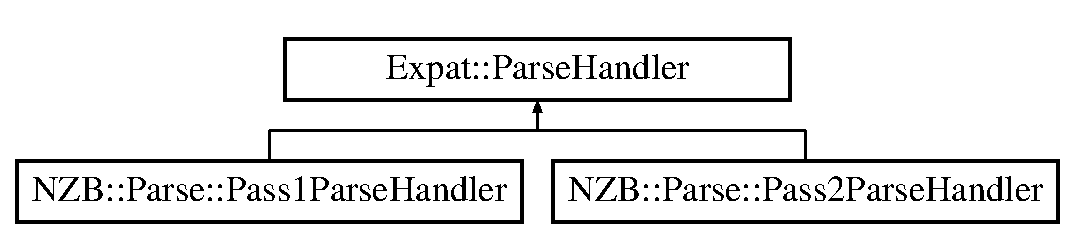
\includegraphics[height=2.000000cm]{class_expat_1_1_parse_handler}
\end{center}
\end{figure}
\subsection*{Public Member Functions}
\begin{DoxyCompactItemize}
\item 
\hyperlink{class_expat_1_1_parse_handler_a0d1e9403a9de36e7f9864a0f665b8b65}{Parse\+Handler} ()
\item 
\hyperlink{class_expat_1_1_parse_handler_a2757b8dca21b50bc9ff8298591cfb6a6}{Parse\+Handler} (const \hyperlink{class_expat_1_1_parse_handler}{Parse\+Handler} \&)=delete
\item 
virtual \hyperlink{class_expat_1_1_parse_handler_a188f81926a657b5231fc4a60a5905701}{$\sim$\+Parse\+Handler} ()
\item 
virtual void \hyperlink{class_expat_1_1_parse_handler_aa6b631d6e771281fb965881545ebacfa}{start\+Element} (const X\+M\+L\+\_\+\+Char $\ast$name, const X\+M\+L\+\_\+\+Char $\ast$$\ast$attrs)
\item 
virtual void \hyperlink{class_expat_1_1_parse_handler_a13c775fa36138b4ee429e10b93177bec}{end\+Element} (const X\+M\+L\+\_\+\+Char $\ast$name)
\item 
virtual void \hyperlink{class_expat_1_1_parse_handler_af3f6effd1ab8b85ec007b981f83d130e}{character\+Data} (const X\+M\+L\+\_\+\+Char $\ast$s, int len)
\item 
virtual void \hyperlink{class_expat_1_1_parse_handler_a7ede3019b6e3eba355504bc34f0143d9}{processing\+Instruction} (const X\+M\+L\+\_\+\+Char $\ast$target, const X\+M\+L\+\_\+\+Char $\ast$data)
\item 
virtual void \hyperlink{class_expat_1_1_parse_handler_a1a4635db36fc5f7abae3deb6ea47becc}{comment} (const X\+M\+L\+\_\+\+Char $\ast$data)
\item 
virtual void \hyperlink{class_expat_1_1_parse_handler_aa839f673fa3b34090b3a6d4341da7df8}{start\+Cdata\+Section} ()
\item 
virtual void \hyperlink{class_expat_1_1_parse_handler_a63611532e55e95c43d074846fdc73314}{end\+Cdata\+Section} ()
\item 
virtual void \hyperlink{class_expat_1_1_parse_handler_a652aca387f4ed68e0178e89b75adb651}{default\+Handler} (const X\+M\+L\+\_\+\+Char $\ast$s, int len)
\item 
virtual int \hyperlink{class_expat_1_1_parse_handler_a54f2787ed9c5134d4a6bf7748a23c3cf}{external\+Entity\+Ref} (const X\+M\+L\+\_\+\+Char $\ast$context, const X\+M\+L\+\_\+\+Char $\ast$base, const X\+M\+L\+\_\+\+Char $\ast$system\+Id, const X\+M\+L\+\_\+\+Char $\ast$public\+Id)
\item 
virtual void \hyperlink{class_expat_1_1_parse_handler_a53aeb5ae280522c3c54a7f78fe660cb0}{skipped\+Entity} (const X\+M\+L\+\_\+\+Char $\ast$entity\+Name, int is\+\_\+parameter\+\_\+entity)
\item 
virtual int \hyperlink{class_expat_1_1_parse_handler_a85918826630176ca85004f828255fdbb}{unknown\+Encoding} (const X\+M\+L\+\_\+\+Char $\ast$name, X\+M\+L\+\_\+\+Encoding $\ast$info)
\item 
virtual void \hyperlink{class_expat_1_1_parse_handler_a24dfc830fb9b782c7a6382725b678954}{start\+Namespace\+Decl} (const X\+M\+L\+\_\+\+Char $\ast$prefix, const X\+M\+L\+\_\+\+Char $\ast$uri)
\item 
virtual void \hyperlink{class_expat_1_1_parse_handler_a143b6a2ac34bbbb46cff621c64d94220}{end\+Namespace\+Decl} (const X\+M\+L\+\_\+\+Char $\ast$prefix)
\item 
virtual void \hyperlink{class_expat_1_1_parse_handler_addc24d4f9b97fd033deb8c1d14d6b9b8}{xml\+Decl} (const X\+M\+L\+\_\+\+Char $\ast$version, const X\+M\+L\+\_\+\+Char $\ast$encoding, int standalone)
\item 
virtual void \hyperlink{class_expat_1_1_parse_handler_a83d12b5e5f35a472655c178000993650}{start\+Doc\+Type} (const X\+M\+L\+\_\+\+Char $\ast$doctype\+Name, const X\+M\+L\+\_\+\+Char $\ast$sysid, const X\+M\+L\+\_\+\+Char $\ast$pubid, int has\+\_\+internal\+\_\+subset)
\item 
virtual void \hyperlink{class_expat_1_1_parse_handler_ad0d1f858b37474da0f634c2d60d94da6}{end\+Doc\+Type} ()
\item 
virtual void \hyperlink{class_expat_1_1_parse_handler_a671fa663133a106e4f9f7c0496ddef5a}{element\+Decl} (const X\+M\+L\+\_\+\+Char $\ast$name, X\+M\+L\+\_\+\+Content $\ast$model)
\item 
virtual void \hyperlink{class_expat_1_1_parse_handler_aef520b46141f4c8249299470de092041}{attlist\+Decl} (const X\+M\+L\+\_\+\+Char $\ast$elname, const X\+M\+L\+\_\+\+Char $\ast$attname, const X\+M\+L\+\_\+\+Char $\ast$att\+\_\+type, const X\+M\+L\+\_\+\+Char $\ast$dflt, int isrequired)
\item 
virtual void \hyperlink{class_expat_1_1_parse_handler_aee63f888e11cae11314311d240ea3b03}{entity\+Decl} (const X\+M\+L\+\_\+\+Char $\ast$entity\+Name, int is\+\_\+parameter\+\_\+entity, const X\+M\+L\+\_\+\+Char $\ast$value, int value\+\_\+length, const X\+M\+L\+\_\+\+Char $\ast$base, const X\+M\+L\+\_\+\+Char $\ast$system\+Id, const X\+M\+L\+\_\+\+Char $\ast$public\+Id, const X\+M\+L\+\_\+\+Char $\ast$notation\+Name)
\item 
virtual void \hyperlink{class_expat_1_1_parse_handler_a0f9bf618ebac7414e88573a743cad783}{notation\+Decl} (const X\+M\+L\+\_\+\+Char $\ast$notation\+Name, const X\+M\+L\+\_\+\+Char $\ast$base, const X\+M\+L\+\_\+\+Char $\ast$system\+Id, const X\+M\+L\+\_\+\+Char $\ast$public\+Id)
\item 
virtual int \hyperlink{class_expat_1_1_parse_handler_afae69dec3184c2cb9265faed9e65fab7}{not\+Standalone} ()
\item 
\hyperlink{class_expat_1_1_parse_handler}{Parse\+Handler} \& \hyperlink{class_expat_1_1_parse_handler_ab294e7d2b95b118a4e7b8d3c3ada78af}{operator=} (const \hyperlink{class_expat_1_1_parse_handler}{Parse\+Handler} \&)=delete
\end{DoxyCompactItemize}


\subsection{Constructor \& Destructor Documentation}
\hypertarget{class_expat_1_1_parse_handler_a0d1e9403a9de36e7f9864a0f665b8b65}{}\label{class_expat_1_1_parse_handler_a0d1e9403a9de36e7f9864a0f665b8b65} 
\index{Expat\+::\+Parse\+Handler@{Expat\+::\+Parse\+Handler}!Parse\+Handler@{Parse\+Handler}}
\index{Parse\+Handler@{Parse\+Handler}!Expat\+::\+Parse\+Handler@{Expat\+::\+Parse\+Handler}}
\subsubsection{\texorpdfstring{Parse\+Handler()}{ParseHandler()}\hspace{0.1cm}{\footnotesize\ttfamily [1/2]}}
{\footnotesize\ttfamily Expat\+::\+Parse\+Handler\+::\+Parse\+Handler (\begin{DoxyParamCaption}{ }\end{DoxyParamCaption})}

\hypertarget{class_expat_1_1_parse_handler_a2757b8dca21b50bc9ff8298591cfb6a6}{}\label{class_expat_1_1_parse_handler_a2757b8dca21b50bc9ff8298591cfb6a6} 
\index{Expat\+::\+Parse\+Handler@{Expat\+::\+Parse\+Handler}!Parse\+Handler@{Parse\+Handler}}
\index{Parse\+Handler@{Parse\+Handler}!Expat\+::\+Parse\+Handler@{Expat\+::\+Parse\+Handler}}
\subsubsection{\texorpdfstring{Parse\+Handler()}{ParseHandler()}\hspace{0.1cm}{\footnotesize\ttfamily [2/2]}}
{\footnotesize\ttfamily Expat\+::\+Parse\+Handler\+::\+Parse\+Handler (\begin{DoxyParamCaption}\item[{const \hyperlink{class_expat_1_1_parse_handler}{Parse\+Handler} \&}]{ }\end{DoxyParamCaption})\hspace{0.3cm}{\ttfamily [delete]}}

\hypertarget{class_expat_1_1_parse_handler_a188f81926a657b5231fc4a60a5905701}{}\label{class_expat_1_1_parse_handler_a188f81926a657b5231fc4a60a5905701} 
\index{Expat\+::\+Parse\+Handler@{Expat\+::\+Parse\+Handler}!````~Parse\+Handler@{$\sim$\+Parse\+Handler}}
\index{````~Parse\+Handler@{$\sim$\+Parse\+Handler}!Expat\+::\+Parse\+Handler@{Expat\+::\+Parse\+Handler}}
\subsubsection{\texorpdfstring{$\sim$\+Parse\+Handler()}{~ParseHandler()}}
{\footnotesize\ttfamily Expat\+::\+Parse\+Handler\+::$\sim$\+Parse\+Handler (\begin{DoxyParamCaption}{ }\end{DoxyParamCaption})\hspace{0.3cm}{\ttfamily [virtual]}}



\subsection{Member Function Documentation}
\hypertarget{class_expat_1_1_parse_handler_aef520b46141f4c8249299470de092041}{}\label{class_expat_1_1_parse_handler_aef520b46141f4c8249299470de092041} 
\index{Expat\+::\+Parse\+Handler@{Expat\+::\+Parse\+Handler}!attlist\+Decl@{attlist\+Decl}}
\index{attlist\+Decl@{attlist\+Decl}!Expat\+::\+Parse\+Handler@{Expat\+::\+Parse\+Handler}}
\subsubsection{\texorpdfstring{attlist\+Decl()}{attlistDecl()}}
{\footnotesize\ttfamily void Expat\+::\+Parse\+Handler\+::attlist\+Decl (\begin{DoxyParamCaption}\item[{const X\+M\+L\+\_\+\+Char $\ast$}]{elname,  }\item[{const X\+M\+L\+\_\+\+Char $\ast$}]{attname,  }\item[{const X\+M\+L\+\_\+\+Char $\ast$}]{att\+\_\+type,  }\item[{const X\+M\+L\+\_\+\+Char $\ast$}]{dflt,  }\item[{int}]{isrequired }\end{DoxyParamCaption})\hspace{0.3cm}{\ttfamily [virtual]}}

\hypertarget{class_expat_1_1_parse_handler_af3f6effd1ab8b85ec007b981f83d130e}{}\label{class_expat_1_1_parse_handler_af3f6effd1ab8b85ec007b981f83d130e} 
\index{Expat\+::\+Parse\+Handler@{Expat\+::\+Parse\+Handler}!character\+Data@{character\+Data}}
\index{character\+Data@{character\+Data}!Expat\+::\+Parse\+Handler@{Expat\+::\+Parse\+Handler}}
\subsubsection{\texorpdfstring{character\+Data()}{characterData()}}
{\footnotesize\ttfamily void Expat\+::\+Parse\+Handler\+::character\+Data (\begin{DoxyParamCaption}\item[{const X\+M\+L\+\_\+\+Char $\ast$}]{s,  }\item[{int}]{len }\end{DoxyParamCaption})\hspace{0.3cm}{\ttfamily [virtual]}}



Reimplemented in \hyperlink{class_n_z_b_1_1_parse_1_1_pass2_parse_handler_adafb3081bcec7653a9b0b3ce8f25a1a5}{N\+Z\+B\+::\+Parse\+::\+Pass2\+Parse\+Handler}.

\hypertarget{class_expat_1_1_parse_handler_a1a4635db36fc5f7abae3deb6ea47becc}{}\label{class_expat_1_1_parse_handler_a1a4635db36fc5f7abae3deb6ea47becc} 
\index{Expat\+::\+Parse\+Handler@{Expat\+::\+Parse\+Handler}!comment@{comment}}
\index{comment@{comment}!Expat\+::\+Parse\+Handler@{Expat\+::\+Parse\+Handler}}
\subsubsection{\texorpdfstring{comment()}{comment()}}
{\footnotesize\ttfamily void Expat\+::\+Parse\+Handler\+::comment (\begin{DoxyParamCaption}\item[{const X\+M\+L\+\_\+\+Char $\ast$}]{data }\end{DoxyParamCaption})\hspace{0.3cm}{\ttfamily [virtual]}}

\hypertarget{class_expat_1_1_parse_handler_a652aca387f4ed68e0178e89b75adb651}{}\label{class_expat_1_1_parse_handler_a652aca387f4ed68e0178e89b75adb651} 
\index{Expat\+::\+Parse\+Handler@{Expat\+::\+Parse\+Handler}!default\+Handler@{default\+Handler}}
\index{default\+Handler@{default\+Handler}!Expat\+::\+Parse\+Handler@{Expat\+::\+Parse\+Handler}}
\subsubsection{\texorpdfstring{default\+Handler()}{defaultHandler()}}
{\footnotesize\ttfamily void Expat\+::\+Parse\+Handler\+::default\+Handler (\begin{DoxyParamCaption}\item[{const X\+M\+L\+\_\+\+Char $\ast$}]{s,  }\item[{int}]{len }\end{DoxyParamCaption})\hspace{0.3cm}{\ttfamily [virtual]}}

\hypertarget{class_expat_1_1_parse_handler_a671fa663133a106e4f9f7c0496ddef5a}{}\label{class_expat_1_1_parse_handler_a671fa663133a106e4f9f7c0496ddef5a} 
\index{Expat\+::\+Parse\+Handler@{Expat\+::\+Parse\+Handler}!element\+Decl@{element\+Decl}}
\index{element\+Decl@{element\+Decl}!Expat\+::\+Parse\+Handler@{Expat\+::\+Parse\+Handler}}
\subsubsection{\texorpdfstring{element\+Decl()}{elementDecl()}}
{\footnotesize\ttfamily void Expat\+::\+Parse\+Handler\+::element\+Decl (\begin{DoxyParamCaption}\item[{const X\+M\+L\+\_\+\+Char $\ast$}]{name,  }\item[{X\+M\+L\+\_\+\+Content $\ast$}]{model }\end{DoxyParamCaption})\hspace{0.3cm}{\ttfamily [virtual]}}

\hypertarget{class_expat_1_1_parse_handler_a63611532e55e95c43d074846fdc73314}{}\label{class_expat_1_1_parse_handler_a63611532e55e95c43d074846fdc73314} 
\index{Expat\+::\+Parse\+Handler@{Expat\+::\+Parse\+Handler}!end\+Cdata\+Section@{end\+Cdata\+Section}}
\index{end\+Cdata\+Section@{end\+Cdata\+Section}!Expat\+::\+Parse\+Handler@{Expat\+::\+Parse\+Handler}}
\subsubsection{\texorpdfstring{end\+Cdata\+Section()}{endCdataSection()}}
{\footnotesize\ttfamily void Expat\+::\+Parse\+Handler\+::end\+Cdata\+Section (\begin{DoxyParamCaption}{ }\end{DoxyParamCaption})\hspace{0.3cm}{\ttfamily [virtual]}}

\hypertarget{class_expat_1_1_parse_handler_ad0d1f858b37474da0f634c2d60d94da6}{}\label{class_expat_1_1_parse_handler_ad0d1f858b37474da0f634c2d60d94da6} 
\index{Expat\+::\+Parse\+Handler@{Expat\+::\+Parse\+Handler}!end\+Doc\+Type@{end\+Doc\+Type}}
\index{end\+Doc\+Type@{end\+Doc\+Type}!Expat\+::\+Parse\+Handler@{Expat\+::\+Parse\+Handler}}
\subsubsection{\texorpdfstring{end\+Doc\+Type()}{endDocType()}}
{\footnotesize\ttfamily void Expat\+::\+Parse\+Handler\+::end\+Doc\+Type (\begin{DoxyParamCaption}{ }\end{DoxyParamCaption})\hspace{0.3cm}{\ttfamily [virtual]}}

\hypertarget{class_expat_1_1_parse_handler_a13c775fa36138b4ee429e10b93177bec}{}\label{class_expat_1_1_parse_handler_a13c775fa36138b4ee429e10b93177bec} 
\index{Expat\+::\+Parse\+Handler@{Expat\+::\+Parse\+Handler}!end\+Element@{end\+Element}}
\index{end\+Element@{end\+Element}!Expat\+::\+Parse\+Handler@{Expat\+::\+Parse\+Handler}}
\subsubsection{\texorpdfstring{end\+Element()}{endElement()}}
{\footnotesize\ttfamily void Expat\+::\+Parse\+Handler\+::end\+Element (\begin{DoxyParamCaption}\item[{const X\+M\+L\+\_\+\+Char $\ast$}]{name }\end{DoxyParamCaption})\hspace{0.3cm}{\ttfamily [virtual]}}



Reimplemented in \hyperlink{class_n_z_b_1_1_parse_1_1_pass2_parse_handler_aadec64ab8a4f9bfd7f3b40bd76cce7aa}{N\+Z\+B\+::\+Parse\+::\+Pass2\+Parse\+Handler}, and \hyperlink{class_n_z_b_1_1_parse_1_1_pass1_parse_handler_afbdd1eaa80a10f66cba06a260fd9e7a1}{N\+Z\+B\+::\+Parse\+::\+Pass1\+Parse\+Handler}.

\hypertarget{class_expat_1_1_parse_handler_a143b6a2ac34bbbb46cff621c64d94220}{}\label{class_expat_1_1_parse_handler_a143b6a2ac34bbbb46cff621c64d94220} 
\index{Expat\+::\+Parse\+Handler@{Expat\+::\+Parse\+Handler}!end\+Namespace\+Decl@{end\+Namespace\+Decl}}
\index{end\+Namespace\+Decl@{end\+Namespace\+Decl}!Expat\+::\+Parse\+Handler@{Expat\+::\+Parse\+Handler}}
\subsubsection{\texorpdfstring{end\+Namespace\+Decl()}{endNamespaceDecl()}}
{\footnotesize\ttfamily void Expat\+::\+Parse\+Handler\+::end\+Namespace\+Decl (\begin{DoxyParamCaption}\item[{const X\+M\+L\+\_\+\+Char $\ast$}]{prefix }\end{DoxyParamCaption})\hspace{0.3cm}{\ttfamily [virtual]}}

\hypertarget{class_expat_1_1_parse_handler_aee63f888e11cae11314311d240ea3b03}{}\label{class_expat_1_1_parse_handler_aee63f888e11cae11314311d240ea3b03} 
\index{Expat\+::\+Parse\+Handler@{Expat\+::\+Parse\+Handler}!entity\+Decl@{entity\+Decl}}
\index{entity\+Decl@{entity\+Decl}!Expat\+::\+Parse\+Handler@{Expat\+::\+Parse\+Handler}}
\subsubsection{\texorpdfstring{entity\+Decl()}{entityDecl()}}
{\footnotesize\ttfamily void Expat\+::\+Parse\+Handler\+::entity\+Decl (\begin{DoxyParamCaption}\item[{const X\+M\+L\+\_\+\+Char $\ast$}]{entity\+Name,  }\item[{int}]{is\+\_\+parameter\+\_\+entity,  }\item[{const X\+M\+L\+\_\+\+Char $\ast$}]{value,  }\item[{int}]{value\+\_\+length,  }\item[{const X\+M\+L\+\_\+\+Char $\ast$}]{base,  }\item[{const X\+M\+L\+\_\+\+Char $\ast$}]{system\+Id,  }\item[{const X\+M\+L\+\_\+\+Char $\ast$}]{public\+Id,  }\item[{const X\+M\+L\+\_\+\+Char $\ast$}]{notation\+Name }\end{DoxyParamCaption})\hspace{0.3cm}{\ttfamily [virtual]}}

\hypertarget{class_expat_1_1_parse_handler_a54f2787ed9c5134d4a6bf7748a23c3cf}{}\label{class_expat_1_1_parse_handler_a54f2787ed9c5134d4a6bf7748a23c3cf} 
\index{Expat\+::\+Parse\+Handler@{Expat\+::\+Parse\+Handler}!external\+Entity\+Ref@{external\+Entity\+Ref}}
\index{external\+Entity\+Ref@{external\+Entity\+Ref}!Expat\+::\+Parse\+Handler@{Expat\+::\+Parse\+Handler}}
\subsubsection{\texorpdfstring{external\+Entity\+Ref()}{externalEntityRef()}}
{\footnotesize\ttfamily int Expat\+::\+Parse\+Handler\+::external\+Entity\+Ref (\begin{DoxyParamCaption}\item[{const X\+M\+L\+\_\+\+Char $\ast$}]{context,  }\item[{const X\+M\+L\+\_\+\+Char $\ast$}]{base,  }\item[{const X\+M\+L\+\_\+\+Char $\ast$}]{system\+Id,  }\item[{const X\+M\+L\+\_\+\+Char $\ast$}]{public\+Id }\end{DoxyParamCaption})\hspace{0.3cm}{\ttfamily [virtual]}}

\hypertarget{class_expat_1_1_parse_handler_a0f9bf618ebac7414e88573a743cad783}{}\label{class_expat_1_1_parse_handler_a0f9bf618ebac7414e88573a743cad783} 
\index{Expat\+::\+Parse\+Handler@{Expat\+::\+Parse\+Handler}!notation\+Decl@{notation\+Decl}}
\index{notation\+Decl@{notation\+Decl}!Expat\+::\+Parse\+Handler@{Expat\+::\+Parse\+Handler}}
\subsubsection{\texorpdfstring{notation\+Decl()}{notationDecl()}}
{\footnotesize\ttfamily void Expat\+::\+Parse\+Handler\+::notation\+Decl (\begin{DoxyParamCaption}\item[{const X\+M\+L\+\_\+\+Char $\ast$}]{notation\+Name,  }\item[{const X\+M\+L\+\_\+\+Char $\ast$}]{base,  }\item[{const X\+M\+L\+\_\+\+Char $\ast$}]{system\+Id,  }\item[{const X\+M\+L\+\_\+\+Char $\ast$}]{public\+Id }\end{DoxyParamCaption})\hspace{0.3cm}{\ttfamily [virtual]}}

\hypertarget{class_expat_1_1_parse_handler_afae69dec3184c2cb9265faed9e65fab7}{}\label{class_expat_1_1_parse_handler_afae69dec3184c2cb9265faed9e65fab7} 
\index{Expat\+::\+Parse\+Handler@{Expat\+::\+Parse\+Handler}!not\+Standalone@{not\+Standalone}}
\index{not\+Standalone@{not\+Standalone}!Expat\+::\+Parse\+Handler@{Expat\+::\+Parse\+Handler}}
\subsubsection{\texorpdfstring{not\+Standalone()}{notStandalone()}}
{\footnotesize\ttfamily int Expat\+::\+Parse\+Handler\+::not\+Standalone (\begin{DoxyParamCaption}{ }\end{DoxyParamCaption})\hspace{0.3cm}{\ttfamily [virtual]}}

\hypertarget{class_expat_1_1_parse_handler_ab294e7d2b95b118a4e7b8d3c3ada78af}{}\label{class_expat_1_1_parse_handler_ab294e7d2b95b118a4e7b8d3c3ada78af} 
\index{Expat\+::\+Parse\+Handler@{Expat\+::\+Parse\+Handler}!operator=@{operator=}}
\index{operator=@{operator=}!Expat\+::\+Parse\+Handler@{Expat\+::\+Parse\+Handler}}
\subsubsection{\texorpdfstring{operator=()}{operator=()}}
{\footnotesize\ttfamily \hyperlink{class_expat_1_1_parse_handler}{Parse\+Handler}\& Expat\+::\+Parse\+Handler\+::operator= (\begin{DoxyParamCaption}\item[{const \hyperlink{class_expat_1_1_parse_handler}{Parse\+Handler} \&}]{ }\end{DoxyParamCaption})\hspace{0.3cm}{\ttfamily [delete]}}

\hypertarget{class_expat_1_1_parse_handler_a7ede3019b6e3eba355504bc34f0143d9}{}\label{class_expat_1_1_parse_handler_a7ede3019b6e3eba355504bc34f0143d9} 
\index{Expat\+::\+Parse\+Handler@{Expat\+::\+Parse\+Handler}!processing\+Instruction@{processing\+Instruction}}
\index{processing\+Instruction@{processing\+Instruction}!Expat\+::\+Parse\+Handler@{Expat\+::\+Parse\+Handler}}
\subsubsection{\texorpdfstring{processing\+Instruction()}{processingInstruction()}}
{\footnotesize\ttfamily void Expat\+::\+Parse\+Handler\+::processing\+Instruction (\begin{DoxyParamCaption}\item[{const X\+M\+L\+\_\+\+Char $\ast$}]{target,  }\item[{const X\+M\+L\+\_\+\+Char $\ast$}]{data }\end{DoxyParamCaption})\hspace{0.3cm}{\ttfamily [virtual]}}

\hypertarget{class_expat_1_1_parse_handler_a53aeb5ae280522c3c54a7f78fe660cb0}{}\label{class_expat_1_1_parse_handler_a53aeb5ae280522c3c54a7f78fe660cb0} 
\index{Expat\+::\+Parse\+Handler@{Expat\+::\+Parse\+Handler}!skipped\+Entity@{skipped\+Entity}}
\index{skipped\+Entity@{skipped\+Entity}!Expat\+::\+Parse\+Handler@{Expat\+::\+Parse\+Handler}}
\subsubsection{\texorpdfstring{skipped\+Entity()}{skippedEntity()}}
{\footnotesize\ttfamily void Expat\+::\+Parse\+Handler\+::skipped\+Entity (\begin{DoxyParamCaption}\item[{const X\+M\+L\+\_\+\+Char $\ast$}]{entity\+Name,  }\item[{int}]{is\+\_\+parameter\+\_\+entity }\end{DoxyParamCaption})\hspace{0.3cm}{\ttfamily [virtual]}}

\hypertarget{class_expat_1_1_parse_handler_aa839f673fa3b34090b3a6d4341da7df8}{}\label{class_expat_1_1_parse_handler_aa839f673fa3b34090b3a6d4341da7df8} 
\index{Expat\+::\+Parse\+Handler@{Expat\+::\+Parse\+Handler}!start\+Cdata\+Section@{start\+Cdata\+Section}}
\index{start\+Cdata\+Section@{start\+Cdata\+Section}!Expat\+::\+Parse\+Handler@{Expat\+::\+Parse\+Handler}}
\subsubsection{\texorpdfstring{start\+Cdata\+Section()}{startCdataSection()}}
{\footnotesize\ttfamily void Expat\+::\+Parse\+Handler\+::start\+Cdata\+Section (\begin{DoxyParamCaption}{ }\end{DoxyParamCaption})\hspace{0.3cm}{\ttfamily [virtual]}}

\hypertarget{class_expat_1_1_parse_handler_a83d12b5e5f35a472655c178000993650}{}\label{class_expat_1_1_parse_handler_a83d12b5e5f35a472655c178000993650} 
\index{Expat\+::\+Parse\+Handler@{Expat\+::\+Parse\+Handler}!start\+Doc\+Type@{start\+Doc\+Type}}
\index{start\+Doc\+Type@{start\+Doc\+Type}!Expat\+::\+Parse\+Handler@{Expat\+::\+Parse\+Handler}}
\subsubsection{\texorpdfstring{start\+Doc\+Type()}{startDocType()}}
{\footnotesize\ttfamily void Expat\+::\+Parse\+Handler\+::start\+Doc\+Type (\begin{DoxyParamCaption}\item[{const X\+M\+L\+\_\+\+Char $\ast$}]{doctype\+Name,  }\item[{const X\+M\+L\+\_\+\+Char $\ast$}]{sysid,  }\item[{const X\+M\+L\+\_\+\+Char $\ast$}]{pubid,  }\item[{int}]{has\+\_\+internal\+\_\+subset }\end{DoxyParamCaption})\hspace{0.3cm}{\ttfamily [virtual]}}

\hypertarget{class_expat_1_1_parse_handler_aa6b631d6e771281fb965881545ebacfa}{}\label{class_expat_1_1_parse_handler_aa6b631d6e771281fb965881545ebacfa} 
\index{Expat\+::\+Parse\+Handler@{Expat\+::\+Parse\+Handler}!start\+Element@{start\+Element}}
\index{start\+Element@{start\+Element}!Expat\+::\+Parse\+Handler@{Expat\+::\+Parse\+Handler}}
\subsubsection{\texorpdfstring{start\+Element()}{startElement()}}
{\footnotesize\ttfamily void Expat\+::\+Parse\+Handler\+::start\+Element (\begin{DoxyParamCaption}\item[{const X\+M\+L\+\_\+\+Char $\ast$}]{name,  }\item[{const X\+M\+L\+\_\+\+Char $\ast$$\ast$}]{attrs }\end{DoxyParamCaption})\hspace{0.3cm}{\ttfamily [virtual]}}



Reimplemented in \hyperlink{class_n_z_b_1_1_parse_1_1_pass2_parse_handler_a2b3ab039352b1bf106d795188d0cd4c1}{N\+Z\+B\+::\+Parse\+::\+Pass2\+Parse\+Handler}.

\hypertarget{class_expat_1_1_parse_handler_a24dfc830fb9b782c7a6382725b678954}{}\label{class_expat_1_1_parse_handler_a24dfc830fb9b782c7a6382725b678954} 
\index{Expat\+::\+Parse\+Handler@{Expat\+::\+Parse\+Handler}!start\+Namespace\+Decl@{start\+Namespace\+Decl}}
\index{start\+Namespace\+Decl@{start\+Namespace\+Decl}!Expat\+::\+Parse\+Handler@{Expat\+::\+Parse\+Handler}}
\subsubsection{\texorpdfstring{start\+Namespace\+Decl()}{startNamespaceDecl()}}
{\footnotesize\ttfamily void Expat\+::\+Parse\+Handler\+::start\+Namespace\+Decl (\begin{DoxyParamCaption}\item[{const X\+M\+L\+\_\+\+Char $\ast$}]{prefix,  }\item[{const X\+M\+L\+\_\+\+Char $\ast$}]{uri }\end{DoxyParamCaption})\hspace{0.3cm}{\ttfamily [virtual]}}

\hypertarget{class_expat_1_1_parse_handler_a85918826630176ca85004f828255fdbb}{}\label{class_expat_1_1_parse_handler_a85918826630176ca85004f828255fdbb} 
\index{Expat\+::\+Parse\+Handler@{Expat\+::\+Parse\+Handler}!unknown\+Encoding@{unknown\+Encoding}}
\index{unknown\+Encoding@{unknown\+Encoding}!Expat\+::\+Parse\+Handler@{Expat\+::\+Parse\+Handler}}
\subsubsection{\texorpdfstring{unknown\+Encoding()}{unknownEncoding()}}
{\footnotesize\ttfamily int Expat\+::\+Parse\+Handler\+::unknown\+Encoding (\begin{DoxyParamCaption}\item[{const X\+M\+L\+\_\+\+Char $\ast$}]{name,  }\item[{X\+M\+L\+\_\+\+Encoding $\ast$}]{info }\end{DoxyParamCaption})\hspace{0.3cm}{\ttfamily [virtual]}}

\hypertarget{class_expat_1_1_parse_handler_addc24d4f9b97fd033deb8c1d14d6b9b8}{}\label{class_expat_1_1_parse_handler_addc24d4f9b97fd033deb8c1d14d6b9b8} 
\index{Expat\+::\+Parse\+Handler@{Expat\+::\+Parse\+Handler}!xml\+Decl@{xml\+Decl}}
\index{xml\+Decl@{xml\+Decl}!Expat\+::\+Parse\+Handler@{Expat\+::\+Parse\+Handler}}
\subsubsection{\texorpdfstring{xml\+Decl()}{xmlDecl()}}
{\footnotesize\ttfamily void Expat\+::\+Parse\+Handler\+::xml\+Decl (\begin{DoxyParamCaption}\item[{const X\+M\+L\+\_\+\+Char $\ast$}]{version,  }\item[{const X\+M\+L\+\_\+\+Char $\ast$}]{encoding,  }\item[{int}]{standalone }\end{DoxyParamCaption})\hspace{0.3cm}{\ttfamily [virtual]}}



The documentation for this class was generated from the following files\+:\begin{DoxyCompactItemize}
\item 
src/\hyperlink{expat_parse_8h}{expat\+Parse.\+h}\item 
src/\hyperlink{expatparse_8cpp}{expatparse.\+cpp}\end{DoxyCompactItemize}

\hypertarget{class_expat_1_1_parser}{}\section{Expat\+:\+:Parser Class Reference}
\label{class_expat_1_1_parser}\index{Expat\+::\+Parser@{Expat\+::\+Parser}}


{\ttfamily \#include $<$expat\+Parse.\+h$>$}

\subsection*{Public Member Functions}
\begin{DoxyCompactItemize}
\item 
\hyperlink{class_expat_1_1_parser_a9bf69dbcb4071a2ff9c63e334d07b92a}{Parser} (const X\+M\+L\+\_\+\+Char $\ast$encoding=N\+U\+LL)
\item 
\hyperlink{class_expat_1_1_parser_a22a2acddfb94bc63872a7168e1957f29}{Parser} (X\+M\+L\+\_\+\+Char separator, const X\+M\+L\+\_\+\+Char $\ast$encoding=N\+U\+LL)
\item 
\hyperlink{class_expat_1_1_parser_a117d15428bc6a06ec163f5b5e3cc9653}{Parser} (const \hyperlink{class_expat_1_1_parser}{Parser} \&)=delete
\item 
virtual \hyperlink{class_expat_1_1_parser_a010a8ab512b43fe40ed79f77363773cc}{$\sim$\+Parser} ()
\item 
void \hyperlink{class_expat_1_1_parser_ab3cf9ce85b9dfc2d5b259ef14e293910}{reset} (const X\+M\+L\+\_\+\+Char $\ast$encoding=N\+U\+LL)
\item 
void \hyperlink{class_expat_1_1_parser_af3ac9195ddabde325e21aa2262e1ca4d}{parse\+File} (\hyperlink{class_expat_1_1_parse_handler}{Parse\+Handler} \&handler, const char $\ast$path)
\item 
void \hyperlink{class_expat_1_1_parser_a7c7133c5ec8f562d1520de8a03918c4d}{parse\+File} (\hyperlink{class_expat_1_1_parse_handler}{Parse\+Handler} \&handler, std\+::istream \&file\+In)
\item 
\hyperlink{class_expat_1_1_parser}{Parser} \& \hyperlink{class_expat_1_1_parser_a5091e3622d34fc04f1f51dd5b48e69af}{operator=} (const \hyperlink{class_expat_1_1_parser}{Parser} \&)=delete
\end{DoxyCompactItemize}
\subsection*{Protected Attributes}
\begin{DoxyCompactItemize}
\item 
X\+M\+L\+\_\+\+Parser \hyperlink{class_expat_1_1_parser_ab4d84cca8e9c64aa1acd96a55a86d62f}{m\+Parser}
\end{DoxyCompactItemize}


\subsection{Constructor \& Destructor Documentation}
\hypertarget{class_expat_1_1_parser_a9bf69dbcb4071a2ff9c63e334d07b92a}{}\label{class_expat_1_1_parser_a9bf69dbcb4071a2ff9c63e334d07b92a} 
\index{Expat\+::\+Parser@{Expat\+::\+Parser}!Parser@{Parser}}
\index{Parser@{Parser}!Expat\+::\+Parser@{Expat\+::\+Parser}}
\subsubsection{\texorpdfstring{Parser()}{Parser()}\hspace{0.1cm}{\footnotesize\ttfamily [1/3]}}
{\footnotesize\ttfamily Expat\+::\+Parser\+::\+Parser (\begin{DoxyParamCaption}\item[{const X\+M\+L\+\_\+\+Char $\ast$}]{encoding = {\ttfamily NULL} }\end{DoxyParamCaption})}

\hypertarget{class_expat_1_1_parser_a22a2acddfb94bc63872a7168e1957f29}{}\label{class_expat_1_1_parser_a22a2acddfb94bc63872a7168e1957f29} 
\index{Expat\+::\+Parser@{Expat\+::\+Parser}!Parser@{Parser}}
\index{Parser@{Parser}!Expat\+::\+Parser@{Expat\+::\+Parser}}
\subsubsection{\texorpdfstring{Parser()}{Parser()}\hspace{0.1cm}{\footnotesize\ttfamily [2/3]}}
{\footnotesize\ttfamily Expat\+::\+Parser\+::\+Parser (\begin{DoxyParamCaption}\item[{X\+M\+L\+\_\+\+Char}]{separator,  }\item[{const X\+M\+L\+\_\+\+Char $\ast$}]{encoding = {\ttfamily NULL} }\end{DoxyParamCaption})}

\hypertarget{class_expat_1_1_parser_a117d15428bc6a06ec163f5b5e3cc9653}{}\label{class_expat_1_1_parser_a117d15428bc6a06ec163f5b5e3cc9653} 
\index{Expat\+::\+Parser@{Expat\+::\+Parser}!Parser@{Parser}}
\index{Parser@{Parser}!Expat\+::\+Parser@{Expat\+::\+Parser}}
\subsubsection{\texorpdfstring{Parser()}{Parser()}\hspace{0.1cm}{\footnotesize\ttfamily [3/3]}}
{\footnotesize\ttfamily Expat\+::\+Parser\+::\+Parser (\begin{DoxyParamCaption}\item[{const \hyperlink{class_expat_1_1_parser}{Parser} \&}]{ }\end{DoxyParamCaption})\hspace{0.3cm}{\ttfamily [delete]}}

\hypertarget{class_expat_1_1_parser_a010a8ab512b43fe40ed79f77363773cc}{}\label{class_expat_1_1_parser_a010a8ab512b43fe40ed79f77363773cc} 
\index{Expat\+::\+Parser@{Expat\+::\+Parser}!````~Parser@{$\sim$\+Parser}}
\index{````~Parser@{$\sim$\+Parser}!Expat\+::\+Parser@{Expat\+::\+Parser}}
\subsubsection{\texorpdfstring{$\sim$\+Parser()}{~Parser()}}
{\footnotesize\ttfamily Expat\+::\+Parser\+::$\sim$\+Parser (\begin{DoxyParamCaption}{ }\end{DoxyParamCaption})\hspace{0.3cm}{\ttfamily [virtual]}}



\subsection{Member Function Documentation}
\hypertarget{class_expat_1_1_parser_a5091e3622d34fc04f1f51dd5b48e69af}{}\label{class_expat_1_1_parser_a5091e3622d34fc04f1f51dd5b48e69af} 
\index{Expat\+::\+Parser@{Expat\+::\+Parser}!operator=@{operator=}}
\index{operator=@{operator=}!Expat\+::\+Parser@{Expat\+::\+Parser}}
\subsubsection{\texorpdfstring{operator=()}{operator=()}}
{\footnotesize\ttfamily \hyperlink{class_expat_1_1_parser}{Parser}\& Expat\+::\+Parser\+::operator= (\begin{DoxyParamCaption}\item[{const \hyperlink{class_expat_1_1_parser}{Parser} \&}]{ }\end{DoxyParamCaption})\hspace{0.3cm}{\ttfamily [delete]}}

\hypertarget{class_expat_1_1_parser_af3ac9195ddabde325e21aa2262e1ca4d}{}\label{class_expat_1_1_parser_af3ac9195ddabde325e21aa2262e1ca4d} 
\index{Expat\+::\+Parser@{Expat\+::\+Parser}!parse\+File@{parse\+File}}
\index{parse\+File@{parse\+File}!Expat\+::\+Parser@{Expat\+::\+Parser}}
\subsubsection{\texorpdfstring{parse\+File()}{parseFile()}\hspace{0.1cm}{\footnotesize\ttfamily [1/2]}}
{\footnotesize\ttfamily void Expat\+::\+Parser\+::parse\+File (\begin{DoxyParamCaption}\item[{\hyperlink{class_expat_1_1_parse_handler}{Parse\+Handler} \&}]{handler,  }\item[{const char $\ast$}]{path }\end{DoxyParamCaption})}

\hypertarget{class_expat_1_1_parser_a7c7133c5ec8f562d1520de8a03918c4d}{}\label{class_expat_1_1_parser_a7c7133c5ec8f562d1520de8a03918c4d} 
\index{Expat\+::\+Parser@{Expat\+::\+Parser}!parse\+File@{parse\+File}}
\index{parse\+File@{parse\+File}!Expat\+::\+Parser@{Expat\+::\+Parser}}
\subsubsection{\texorpdfstring{parse\+File()}{parseFile()}\hspace{0.1cm}{\footnotesize\ttfamily [2/2]}}
{\footnotesize\ttfamily void Expat\+::\+Parser\+::parse\+File (\begin{DoxyParamCaption}\item[{\hyperlink{class_expat_1_1_parse_handler}{Parse\+Handler} \&}]{handler,  }\item[{std\+::istream \&}]{file\+In }\end{DoxyParamCaption})}

\hypertarget{class_expat_1_1_parser_ab3cf9ce85b9dfc2d5b259ef14e293910}{}\label{class_expat_1_1_parser_ab3cf9ce85b9dfc2d5b259ef14e293910} 
\index{Expat\+::\+Parser@{Expat\+::\+Parser}!reset@{reset}}
\index{reset@{reset}!Expat\+::\+Parser@{Expat\+::\+Parser}}
\subsubsection{\texorpdfstring{reset()}{reset()}}
{\footnotesize\ttfamily void Expat\+::\+Parser\+::reset (\begin{DoxyParamCaption}\item[{const X\+M\+L\+\_\+\+Char $\ast$}]{encoding = {\ttfamily NULL} }\end{DoxyParamCaption})}



\subsection{Member Data Documentation}
\hypertarget{class_expat_1_1_parser_ab4d84cca8e9c64aa1acd96a55a86d62f}{}\label{class_expat_1_1_parser_ab4d84cca8e9c64aa1acd96a55a86d62f} 
\index{Expat\+::\+Parser@{Expat\+::\+Parser}!m\+Parser@{m\+Parser}}
\index{m\+Parser@{m\+Parser}!Expat\+::\+Parser@{Expat\+::\+Parser}}
\subsubsection{\texorpdfstring{m\+Parser}{mParser}}
{\footnotesize\ttfamily X\+M\+L\+\_\+\+Parser Expat\+::\+Parser\+::m\+Parser\hspace{0.3cm}{\ttfamily [protected]}}



The documentation for this class was generated from the following files\+:\begin{DoxyCompactItemize}
\item 
src/\hyperlink{expat_parse_8h}{expat\+Parse.\+h}\item 
src/\hyperlink{expatparse_8cpp}{expatparse.\+cpp}\end{DoxyCompactItemize}

\hypertarget{class_n_z_b_1_1_parse_1_1_pass1_parse_handler}{}\section{N\+ZB\+:\+:Parse\+:\+:Pass1\+Parse\+Handler Class Reference}
\label{class_n_z_b_1_1_parse_1_1_pass1_parse_handler}\index{N\+Z\+B\+::\+Parse\+::\+Pass1\+Parse\+Handler@{N\+Z\+B\+::\+Parse\+::\+Pass1\+Parse\+Handler}}
Inheritance diagram for N\+ZB\+:\+:Parse\+:\+:Pass1\+Parse\+Handler\+:\begin{figure}[H]
\begin{center}
\leavevmode
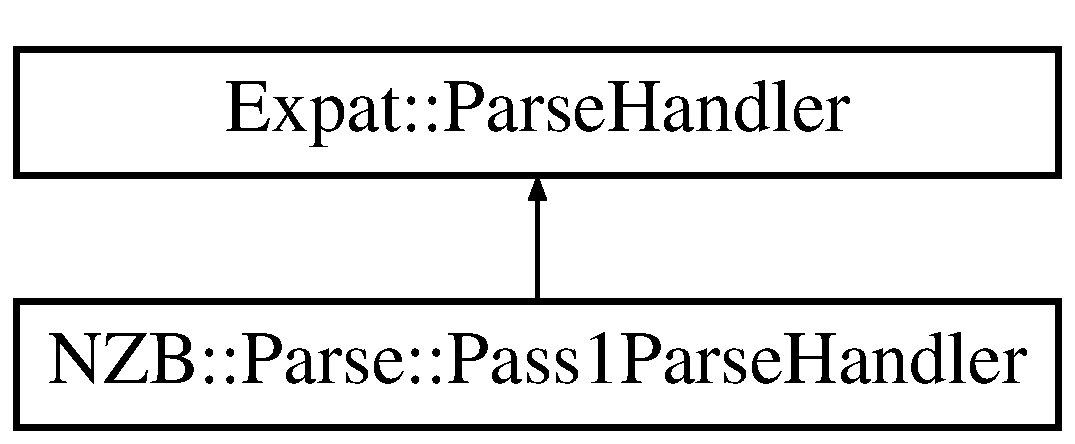
\includegraphics[height=2.000000cm]{class_n_z_b_1_1_parse_1_1_pass1_parse_handler}
\end{center}
\end{figure}
\subsection*{Public Member Functions}
\begin{DoxyCompactItemize}
\item 
\hyperlink{class_n_z_b_1_1_parse_1_1_pass1_parse_handler_a1be458058a48e975914ed8f418828a6b}{Pass1\+Parse\+Handler} ()
\item 
\hyperlink{class_n_z_b_1_1_parse_1_1_pass1_parse_handler_a1dbe3658043ecc45b5fc8aabf923ebf8}{$\sim$\+Pass1\+Parse\+Handler} ()
\item 
int \hyperlink{class_n_z_b_1_1_parse_1_1_pass1_parse_handler_a4e04669e3a8fc7d4c07f7e308de489e5}{get\+Segment\+Count} () const
\item 
int \hyperlink{class_n_z_b_1_1_parse_1_1_pass1_parse_handler_a5ba1c886f45e0340dc22075f99ff51df}{get\+Group\+Count} () const
\item 
int \hyperlink{class_n_z_b_1_1_parse_1_1_pass1_parse_handler_ae61ae9069c299a17793e845c6ab1bbe5}{get\+File\+Count} () const
\item 
void \hyperlink{class_n_z_b_1_1_parse_1_1_pass1_parse_handler_afbdd1eaa80a10f66cba06a260fd9e7a1}{end\+Element} (const X\+M\+L\+\_\+\+Char $\ast$name)
\end{DoxyCompactItemize}
\subsection*{Protected Attributes}
\begin{DoxyCompactItemize}
\item 
int \hyperlink{class_n_z_b_1_1_parse_1_1_pass1_parse_handler_a4160b3aae47236e9b34418de1d162152}{m\+Segment\+Count}
\item 
int \hyperlink{class_n_z_b_1_1_parse_1_1_pass1_parse_handler_a7ad7ebf07c7b22638e26d747b3bd9281}{m\+Group\+Count}
\item 
int \hyperlink{class_n_z_b_1_1_parse_1_1_pass1_parse_handler_ad097bc8568270c31a3483b5488e900d4}{m\+File\+Count}
\end{DoxyCompactItemize}


\subsection{Constructor \& Destructor Documentation}
\hypertarget{class_n_z_b_1_1_parse_1_1_pass1_parse_handler_a1be458058a48e975914ed8f418828a6b}{}\label{class_n_z_b_1_1_parse_1_1_pass1_parse_handler_a1be458058a48e975914ed8f418828a6b} 
\index{N\+Z\+B\+::\+Parse\+::\+Pass1\+Parse\+Handler@{N\+Z\+B\+::\+Parse\+::\+Pass1\+Parse\+Handler}!Pass1\+Parse\+Handler@{Pass1\+Parse\+Handler}}
\index{Pass1\+Parse\+Handler@{Pass1\+Parse\+Handler}!N\+Z\+B\+::\+Parse\+::\+Pass1\+Parse\+Handler@{N\+Z\+B\+::\+Parse\+::\+Pass1\+Parse\+Handler}}
\subsubsection{\texorpdfstring{Pass1\+Parse\+Handler()}{Pass1ParseHandler()}}
{\footnotesize\ttfamily N\+Z\+B\+::\+Parse\+::\+Pass1\+Parse\+Handler\+::\+Pass1\+Parse\+Handler (\begin{DoxyParamCaption}{ }\end{DoxyParamCaption})}

\hypertarget{class_n_z_b_1_1_parse_1_1_pass1_parse_handler_a1dbe3658043ecc45b5fc8aabf923ebf8}{}\label{class_n_z_b_1_1_parse_1_1_pass1_parse_handler_a1dbe3658043ecc45b5fc8aabf923ebf8} 
\index{N\+Z\+B\+::\+Parse\+::\+Pass1\+Parse\+Handler@{N\+Z\+B\+::\+Parse\+::\+Pass1\+Parse\+Handler}!````~Pass1\+Parse\+Handler@{$\sim$\+Pass1\+Parse\+Handler}}
\index{````~Pass1\+Parse\+Handler@{$\sim$\+Pass1\+Parse\+Handler}!N\+Z\+B\+::\+Parse\+::\+Pass1\+Parse\+Handler@{N\+Z\+B\+::\+Parse\+::\+Pass1\+Parse\+Handler}}
\subsubsection{\texorpdfstring{$\sim$\+Pass1\+Parse\+Handler()}{~Pass1ParseHandler()}}
{\footnotesize\ttfamily N\+Z\+B\+::\+Parse\+::\+Pass1\+Parse\+Handler\+::$\sim$\+Pass1\+Parse\+Handler (\begin{DoxyParamCaption}{ }\end{DoxyParamCaption})\hspace{0.3cm}{\ttfamily [inline]}}



\subsection{Member Function Documentation}
\hypertarget{class_n_z_b_1_1_parse_1_1_pass1_parse_handler_afbdd1eaa80a10f66cba06a260fd9e7a1}{}\label{class_n_z_b_1_1_parse_1_1_pass1_parse_handler_afbdd1eaa80a10f66cba06a260fd9e7a1} 
\index{N\+Z\+B\+::\+Parse\+::\+Pass1\+Parse\+Handler@{N\+Z\+B\+::\+Parse\+::\+Pass1\+Parse\+Handler}!end\+Element@{end\+Element}}
\index{end\+Element@{end\+Element}!N\+Z\+B\+::\+Parse\+::\+Pass1\+Parse\+Handler@{N\+Z\+B\+::\+Parse\+::\+Pass1\+Parse\+Handler}}
\subsubsection{\texorpdfstring{end\+Element()}{endElement()}}
{\footnotesize\ttfamily void N\+Z\+B\+::\+Parse\+::\+Pass1\+Parse\+Handler\+::end\+Element (\begin{DoxyParamCaption}\item[{const X\+M\+L\+\_\+\+Char $\ast$}]{name }\end{DoxyParamCaption})\hspace{0.3cm}{\ttfamily [virtual]}}



Reimplemented from \hyperlink{class_expat_1_1_parse_handler_a13c775fa36138b4ee429e10b93177bec}{Expat\+::\+Parse\+Handler}.

\hypertarget{class_n_z_b_1_1_parse_1_1_pass1_parse_handler_ae61ae9069c299a17793e845c6ab1bbe5}{}\label{class_n_z_b_1_1_parse_1_1_pass1_parse_handler_ae61ae9069c299a17793e845c6ab1bbe5} 
\index{N\+Z\+B\+::\+Parse\+::\+Pass1\+Parse\+Handler@{N\+Z\+B\+::\+Parse\+::\+Pass1\+Parse\+Handler}!get\+File\+Count@{get\+File\+Count}}
\index{get\+File\+Count@{get\+File\+Count}!N\+Z\+B\+::\+Parse\+::\+Pass1\+Parse\+Handler@{N\+Z\+B\+::\+Parse\+::\+Pass1\+Parse\+Handler}}
\subsubsection{\texorpdfstring{get\+File\+Count()}{getFileCount()}}
{\footnotesize\ttfamily int N\+Z\+B\+::\+Parse\+::\+Pass1\+Parse\+Handler\+::get\+File\+Count (\begin{DoxyParamCaption}{ }\end{DoxyParamCaption}) const\hspace{0.3cm}{\ttfamily [inline]}}

\hypertarget{class_n_z_b_1_1_parse_1_1_pass1_parse_handler_a5ba1c886f45e0340dc22075f99ff51df}{}\label{class_n_z_b_1_1_parse_1_1_pass1_parse_handler_a5ba1c886f45e0340dc22075f99ff51df} 
\index{N\+Z\+B\+::\+Parse\+::\+Pass1\+Parse\+Handler@{N\+Z\+B\+::\+Parse\+::\+Pass1\+Parse\+Handler}!get\+Group\+Count@{get\+Group\+Count}}
\index{get\+Group\+Count@{get\+Group\+Count}!N\+Z\+B\+::\+Parse\+::\+Pass1\+Parse\+Handler@{N\+Z\+B\+::\+Parse\+::\+Pass1\+Parse\+Handler}}
\subsubsection{\texorpdfstring{get\+Group\+Count()}{getGroupCount()}}
{\footnotesize\ttfamily int N\+Z\+B\+::\+Parse\+::\+Pass1\+Parse\+Handler\+::get\+Group\+Count (\begin{DoxyParamCaption}{ }\end{DoxyParamCaption}) const\hspace{0.3cm}{\ttfamily [inline]}}

\hypertarget{class_n_z_b_1_1_parse_1_1_pass1_parse_handler_a4e04669e3a8fc7d4c07f7e308de489e5}{}\label{class_n_z_b_1_1_parse_1_1_pass1_parse_handler_a4e04669e3a8fc7d4c07f7e308de489e5} 
\index{N\+Z\+B\+::\+Parse\+::\+Pass1\+Parse\+Handler@{N\+Z\+B\+::\+Parse\+::\+Pass1\+Parse\+Handler}!get\+Segment\+Count@{get\+Segment\+Count}}
\index{get\+Segment\+Count@{get\+Segment\+Count}!N\+Z\+B\+::\+Parse\+::\+Pass1\+Parse\+Handler@{N\+Z\+B\+::\+Parse\+::\+Pass1\+Parse\+Handler}}
\subsubsection{\texorpdfstring{get\+Segment\+Count()}{getSegmentCount()}}
{\footnotesize\ttfamily int N\+Z\+B\+::\+Parse\+::\+Pass1\+Parse\+Handler\+::get\+Segment\+Count (\begin{DoxyParamCaption}{ }\end{DoxyParamCaption}) const\hspace{0.3cm}{\ttfamily [inline]}}



\subsection{Member Data Documentation}
\hypertarget{class_n_z_b_1_1_parse_1_1_pass1_parse_handler_ad097bc8568270c31a3483b5488e900d4}{}\label{class_n_z_b_1_1_parse_1_1_pass1_parse_handler_ad097bc8568270c31a3483b5488e900d4} 
\index{N\+Z\+B\+::\+Parse\+::\+Pass1\+Parse\+Handler@{N\+Z\+B\+::\+Parse\+::\+Pass1\+Parse\+Handler}!m\+File\+Count@{m\+File\+Count}}
\index{m\+File\+Count@{m\+File\+Count}!N\+Z\+B\+::\+Parse\+::\+Pass1\+Parse\+Handler@{N\+Z\+B\+::\+Parse\+::\+Pass1\+Parse\+Handler}}
\subsubsection{\texorpdfstring{m\+File\+Count}{mFileCount}}
{\footnotesize\ttfamily int N\+Z\+B\+::\+Parse\+::\+Pass1\+Parse\+Handler\+::m\+File\+Count\hspace{0.3cm}{\ttfamily [protected]}}

\hypertarget{class_n_z_b_1_1_parse_1_1_pass1_parse_handler_a7ad7ebf07c7b22638e26d747b3bd9281}{}\label{class_n_z_b_1_1_parse_1_1_pass1_parse_handler_a7ad7ebf07c7b22638e26d747b3bd9281} 
\index{N\+Z\+B\+::\+Parse\+::\+Pass1\+Parse\+Handler@{N\+Z\+B\+::\+Parse\+::\+Pass1\+Parse\+Handler}!m\+Group\+Count@{m\+Group\+Count}}
\index{m\+Group\+Count@{m\+Group\+Count}!N\+Z\+B\+::\+Parse\+::\+Pass1\+Parse\+Handler@{N\+Z\+B\+::\+Parse\+::\+Pass1\+Parse\+Handler}}
\subsubsection{\texorpdfstring{m\+Group\+Count}{mGroupCount}}
{\footnotesize\ttfamily int N\+Z\+B\+::\+Parse\+::\+Pass1\+Parse\+Handler\+::m\+Group\+Count\hspace{0.3cm}{\ttfamily [protected]}}

\hypertarget{class_n_z_b_1_1_parse_1_1_pass1_parse_handler_a4160b3aae47236e9b34418de1d162152}{}\label{class_n_z_b_1_1_parse_1_1_pass1_parse_handler_a4160b3aae47236e9b34418de1d162152} 
\index{N\+Z\+B\+::\+Parse\+::\+Pass1\+Parse\+Handler@{N\+Z\+B\+::\+Parse\+::\+Pass1\+Parse\+Handler}!m\+Segment\+Count@{m\+Segment\+Count}}
\index{m\+Segment\+Count@{m\+Segment\+Count}!N\+Z\+B\+::\+Parse\+::\+Pass1\+Parse\+Handler@{N\+Z\+B\+::\+Parse\+::\+Pass1\+Parse\+Handler}}
\subsubsection{\texorpdfstring{m\+Segment\+Count}{mSegmentCount}}
{\footnotesize\ttfamily int N\+Z\+B\+::\+Parse\+::\+Pass1\+Parse\+Handler\+::m\+Segment\+Count\hspace{0.3cm}{\ttfamily [protected]}}



The documentation for this class was generated from the following file\+:\begin{DoxyCompactItemize}
\item 
src/\hyperlink{nzbparse_8cpp}{nzbparse.\+cpp}\end{DoxyCompactItemize}

\hypertarget{class_n_z_b_1_1_parse_1_1_pass2_parse_handler}{}\section{N\+ZB\+:\+:Parse\+:\+:Pass2\+Parse\+Handler Class Reference}
\label{class_n_z_b_1_1_parse_1_1_pass2_parse_handler}\index{N\+Z\+B\+::\+Parse\+::\+Pass2\+Parse\+Handler@{N\+Z\+B\+::\+Parse\+::\+Pass2\+Parse\+Handler}}
Inheritance diagram for N\+ZB\+:\+:Parse\+:\+:Pass2\+Parse\+Handler\+:\begin{figure}[H]
\begin{center}
\leavevmode
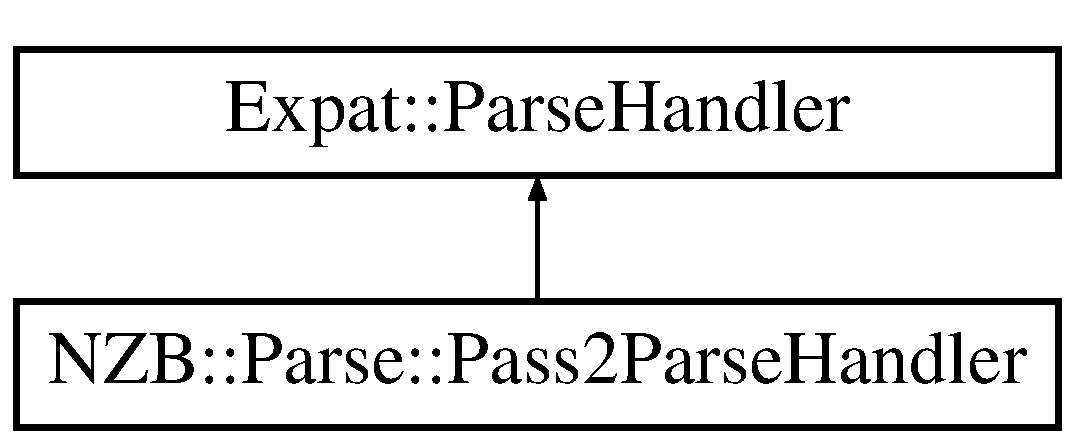
\includegraphics[height=2.000000cm]{class_n_z_b_1_1_parse_1_1_pass2_parse_handler}
\end{center}
\end{figure}
\subsection*{Public Member Functions}
\begin{DoxyCompactItemize}
\item 
\hyperlink{class_n_z_b_1_1_parse_1_1_pass2_parse_handler_a04b11c88f54b2804e13043c5cd57e0d7}{Pass2\+Parse\+Handler} (\hyperlink{class_n_z_b_1_1_file}{N\+Z\+B\+::\+File} $\ast$p\+Files, \hyperlink{class_n_z_b_1_1_segment}{N\+Z\+B\+::\+Segment} $\ast$p\+Segments, \hyperlink{class_n_z_b_1_1_group}{N\+Z\+B\+::\+Group} $\ast$p\+Groups)
\item 
\hyperlink{class_n_z_b_1_1_parse_1_1_pass2_parse_handler_aeda10efa356a2b6ef318a37684206f6c}{$\sim$\+Pass2\+Parse\+Handler} ()
\item 
void \hyperlink{class_n_z_b_1_1_parse_1_1_pass2_parse_handler_a2b3ab039352b1bf106d795188d0cd4c1}{start\+Element} (const X\+M\+L\+\_\+\+Char $\ast$name, const X\+M\+L\+\_\+\+Char $\ast$$\ast$attr)
\item 
void \hyperlink{class_n_z_b_1_1_parse_1_1_pass2_parse_handler_aadec64ab8a4f9bfd7f3b40bd76cce7aa}{end\+Element} (const X\+M\+L\+\_\+\+Char $\ast$name)
\item 
void \hyperlink{class_n_z_b_1_1_parse_1_1_pass2_parse_handler_adafb3081bcec7653a9b0b3ce8f25a1a5}{character\+Data} (const X\+M\+L\+\_\+\+Char $\ast$s, int len)
\end{DoxyCompactItemize}
\subsection*{Protected Types}
\begin{DoxyCompactItemize}
\item 
enum \hyperlink{class_n_z_b_1_1_parse_1_1_pass2_parse_handler_a05e6d45260e206949b805d1f8bb24cc5}{Nzb\+Elem} \{ \hyperlink{class_n_z_b_1_1_parse_1_1_pass2_parse_handler_a05e6d45260e206949b805d1f8bb24cc5aaa618133f4061942ff5b37fd61c800c2}{N\+O\+NE}, 
\hyperlink{class_n_z_b_1_1_parse_1_1_pass2_parse_handler_a05e6d45260e206949b805d1f8bb24cc5a744ce3f7aac22b510695bbe70802fc99}{S\+E\+G\+M\+E\+NT}, 
\hyperlink{class_n_z_b_1_1_parse_1_1_pass2_parse_handler_a05e6d45260e206949b805d1f8bb24cc5a66293d68619d407485329c5ce517f19e}{G\+R\+O\+UP}, 
\hyperlink{class_n_z_b_1_1_parse_1_1_pass2_parse_handler_a05e6d45260e206949b805d1f8bb24cc5ab4ed997bce5cb2f78291e2c277e68e21}{N\+Z\+B\+F\+I\+LE}
 \}
\end{DoxyCompactItemize}
\subsection*{Protected Attributes}
\begin{DoxyCompactItemize}
\item 
\hyperlink{class_n_z_b_1_1_parse_1_1_pass2_parse_handler_a05e6d45260e206949b805d1f8bb24cc5}{Nzb\+Elem} \hyperlink{class_n_z_b_1_1_parse_1_1_pass2_parse_handler_a9c826c2393e2f8d76d8ee1d0a126368e}{m\+Cur\+Elem}
\item 
\hyperlink{class_n_z_b_1_1_file}{N\+Z\+B\+::\+File} $\ast$ \hyperlink{class_n_z_b_1_1_parse_1_1_pass2_parse_handler_aed1cb652f2f9f66446634b487c88f2d0}{mp\+Files}
\item 
\hyperlink{class_n_z_b_1_1_segment}{N\+Z\+B\+::\+Segment} $\ast$ \hyperlink{class_n_z_b_1_1_parse_1_1_pass2_parse_handler_af89a59538b17bf8b840e71c95c97f810}{mp\+Segments}
\item 
\hyperlink{class_n_z_b_1_1_group}{N\+Z\+B\+::\+Group} $\ast$ \hyperlink{class_n_z_b_1_1_parse_1_1_pass2_parse_handler_a04f7ef1c4c7547c15c49d81e7c404f85}{mp\+Groups}
\item 
int \hyperlink{class_n_z_b_1_1_parse_1_1_pass2_parse_handler_aac119e2e3690065b009cd53c21702ec6}{mi\+File}
\item 
int \hyperlink{class_n_z_b_1_1_parse_1_1_pass2_parse_handler_aac2dbf285dc01b72a7cda4e883fcb5b9}{mi\+Segment}
\item 
int \hyperlink{class_n_z_b_1_1_parse_1_1_pass2_parse_handler_afd21564b9f52f71c12e6335140b849bd}{mi\+Segment\+Begin}
\item 
int \hyperlink{class_n_z_b_1_1_parse_1_1_pass2_parse_handler_a126d86f68bf8209f2f7b3aa6e9048bc3}{mi\+Group}
\item 
int \hyperlink{class_n_z_b_1_1_parse_1_1_pass2_parse_handler_afa0b65267cec4fcf26ca934a66c3cc06}{mi\+Group\+Begin}
\item 
std\+::string \hyperlink{class_n_z_b_1_1_parse_1_1_pass2_parse_handler_a3e2bb4640047a0aa35ab93fb1a25465b}{m\+Chars}
\end{DoxyCompactItemize}


\subsection{Member Enumeration Documentation}
\hypertarget{class_n_z_b_1_1_parse_1_1_pass2_parse_handler_a05e6d45260e206949b805d1f8bb24cc5}{}\label{class_n_z_b_1_1_parse_1_1_pass2_parse_handler_a05e6d45260e206949b805d1f8bb24cc5} 
\index{N\+Z\+B\+::\+Parse\+::\+Pass2\+Parse\+Handler@{N\+Z\+B\+::\+Parse\+::\+Pass2\+Parse\+Handler}!Nzb\+Elem@{Nzb\+Elem}}
\index{Nzb\+Elem@{Nzb\+Elem}!N\+Z\+B\+::\+Parse\+::\+Pass2\+Parse\+Handler@{N\+Z\+B\+::\+Parse\+::\+Pass2\+Parse\+Handler}}
\subsubsection{\texorpdfstring{Nzb\+Elem}{NzbElem}}
{\footnotesize\ttfamily enum \hyperlink{class_n_z_b_1_1_parse_1_1_pass2_parse_handler_a05e6d45260e206949b805d1f8bb24cc5}{N\+Z\+B\+::\+Parse\+::\+Pass2\+Parse\+Handler\+::\+Nzb\+Elem}\hspace{0.3cm}{\ttfamily [protected]}}

\begin{DoxyEnumFields}{Enumerator}
\raisebox{\heightof{T}}[0pt][0pt]{\index{N\+O\+NE@{N\+O\+NE}!N\+Z\+B\+::\+Parse\+::\+Pass2\+Parse\+Handler@{N\+Z\+B\+::\+Parse\+::\+Pass2\+Parse\+Handler}}\index{N\+Z\+B\+::\+Parse\+::\+Pass2\+Parse\+Handler@{N\+Z\+B\+::\+Parse\+::\+Pass2\+Parse\+Handler}!N\+O\+NE@{N\+O\+NE}}}\hypertarget{class_n_z_b_1_1_parse_1_1_pass2_parse_handler_a05e6d45260e206949b805d1f8bb24cc5aaa618133f4061942ff5b37fd61c800c2}{}\label{class_n_z_b_1_1_parse_1_1_pass2_parse_handler_a05e6d45260e206949b805d1f8bb24cc5aaa618133f4061942ff5b37fd61c800c2} 
N\+O\+NE&\\
\hline

\raisebox{\heightof{T}}[0pt][0pt]{\index{S\+E\+G\+M\+E\+NT@{S\+E\+G\+M\+E\+NT}!N\+Z\+B\+::\+Parse\+::\+Pass2\+Parse\+Handler@{N\+Z\+B\+::\+Parse\+::\+Pass2\+Parse\+Handler}}\index{N\+Z\+B\+::\+Parse\+::\+Pass2\+Parse\+Handler@{N\+Z\+B\+::\+Parse\+::\+Pass2\+Parse\+Handler}!S\+E\+G\+M\+E\+NT@{S\+E\+G\+M\+E\+NT}}}\hypertarget{class_n_z_b_1_1_parse_1_1_pass2_parse_handler_a05e6d45260e206949b805d1f8bb24cc5a744ce3f7aac22b510695bbe70802fc99}{}\label{class_n_z_b_1_1_parse_1_1_pass2_parse_handler_a05e6d45260e206949b805d1f8bb24cc5a744ce3f7aac22b510695bbe70802fc99} 
S\+E\+G\+M\+E\+NT&\\
\hline

\raisebox{\heightof{T}}[0pt][0pt]{\index{G\+R\+O\+UP@{G\+R\+O\+UP}!N\+Z\+B\+::\+Parse\+::\+Pass2\+Parse\+Handler@{N\+Z\+B\+::\+Parse\+::\+Pass2\+Parse\+Handler}}\index{N\+Z\+B\+::\+Parse\+::\+Pass2\+Parse\+Handler@{N\+Z\+B\+::\+Parse\+::\+Pass2\+Parse\+Handler}!G\+R\+O\+UP@{G\+R\+O\+UP}}}\hypertarget{class_n_z_b_1_1_parse_1_1_pass2_parse_handler_a05e6d45260e206949b805d1f8bb24cc5a66293d68619d407485329c5ce517f19e}{}\label{class_n_z_b_1_1_parse_1_1_pass2_parse_handler_a05e6d45260e206949b805d1f8bb24cc5a66293d68619d407485329c5ce517f19e} 
G\+R\+O\+UP&\\
\hline

\raisebox{\heightof{T}}[0pt][0pt]{\index{N\+Z\+B\+F\+I\+LE@{N\+Z\+B\+F\+I\+LE}!N\+Z\+B\+::\+Parse\+::\+Pass2\+Parse\+Handler@{N\+Z\+B\+::\+Parse\+::\+Pass2\+Parse\+Handler}}\index{N\+Z\+B\+::\+Parse\+::\+Pass2\+Parse\+Handler@{N\+Z\+B\+::\+Parse\+::\+Pass2\+Parse\+Handler}!N\+Z\+B\+F\+I\+LE@{N\+Z\+B\+F\+I\+LE}}}\hypertarget{class_n_z_b_1_1_parse_1_1_pass2_parse_handler_a05e6d45260e206949b805d1f8bb24cc5ab4ed997bce5cb2f78291e2c277e68e21}{}\label{class_n_z_b_1_1_parse_1_1_pass2_parse_handler_a05e6d45260e206949b805d1f8bb24cc5ab4ed997bce5cb2f78291e2c277e68e21} 
N\+Z\+B\+F\+I\+LE&\\
\hline

\end{DoxyEnumFields}


\subsection{Constructor \& Destructor Documentation}
\hypertarget{class_n_z_b_1_1_parse_1_1_pass2_parse_handler_a04b11c88f54b2804e13043c5cd57e0d7}{}\label{class_n_z_b_1_1_parse_1_1_pass2_parse_handler_a04b11c88f54b2804e13043c5cd57e0d7} 
\index{N\+Z\+B\+::\+Parse\+::\+Pass2\+Parse\+Handler@{N\+Z\+B\+::\+Parse\+::\+Pass2\+Parse\+Handler}!Pass2\+Parse\+Handler@{Pass2\+Parse\+Handler}}
\index{Pass2\+Parse\+Handler@{Pass2\+Parse\+Handler}!N\+Z\+B\+::\+Parse\+::\+Pass2\+Parse\+Handler@{N\+Z\+B\+::\+Parse\+::\+Pass2\+Parse\+Handler}}
\subsubsection{\texorpdfstring{Pass2\+Parse\+Handler()}{Pass2ParseHandler()}}
{\footnotesize\ttfamily N\+Z\+B\+::\+Parse\+::\+Pass2\+Parse\+Handler\+::\+Pass2\+Parse\+Handler (\begin{DoxyParamCaption}\item[{\hyperlink{class_n_z_b_1_1_file}{N\+Z\+B\+::\+File} $\ast$}]{p\+Files,  }\item[{\hyperlink{class_n_z_b_1_1_segment}{N\+Z\+B\+::\+Segment} $\ast$}]{p\+Segments,  }\item[{\hyperlink{class_n_z_b_1_1_group}{N\+Z\+B\+::\+Group} $\ast$}]{p\+Groups }\end{DoxyParamCaption})}

\hypertarget{class_n_z_b_1_1_parse_1_1_pass2_parse_handler_aeda10efa356a2b6ef318a37684206f6c}{}\label{class_n_z_b_1_1_parse_1_1_pass2_parse_handler_aeda10efa356a2b6ef318a37684206f6c} 
\index{N\+Z\+B\+::\+Parse\+::\+Pass2\+Parse\+Handler@{N\+Z\+B\+::\+Parse\+::\+Pass2\+Parse\+Handler}!````~Pass2\+Parse\+Handler@{$\sim$\+Pass2\+Parse\+Handler}}
\index{````~Pass2\+Parse\+Handler@{$\sim$\+Pass2\+Parse\+Handler}!N\+Z\+B\+::\+Parse\+::\+Pass2\+Parse\+Handler@{N\+Z\+B\+::\+Parse\+::\+Pass2\+Parse\+Handler}}
\subsubsection{\texorpdfstring{$\sim$\+Pass2\+Parse\+Handler()}{~Pass2ParseHandler()}}
{\footnotesize\ttfamily N\+Z\+B\+::\+Parse\+::\+Pass2\+Parse\+Handler\+::$\sim$\+Pass2\+Parse\+Handler (\begin{DoxyParamCaption}{ }\end{DoxyParamCaption})\hspace{0.3cm}{\ttfamily [inline]}}



\subsection{Member Function Documentation}
\hypertarget{class_n_z_b_1_1_parse_1_1_pass2_parse_handler_adafb3081bcec7653a9b0b3ce8f25a1a5}{}\label{class_n_z_b_1_1_parse_1_1_pass2_parse_handler_adafb3081bcec7653a9b0b3ce8f25a1a5} 
\index{N\+Z\+B\+::\+Parse\+::\+Pass2\+Parse\+Handler@{N\+Z\+B\+::\+Parse\+::\+Pass2\+Parse\+Handler}!character\+Data@{character\+Data}}
\index{character\+Data@{character\+Data}!N\+Z\+B\+::\+Parse\+::\+Pass2\+Parse\+Handler@{N\+Z\+B\+::\+Parse\+::\+Pass2\+Parse\+Handler}}
\subsubsection{\texorpdfstring{character\+Data()}{characterData()}}
{\footnotesize\ttfamily void N\+Z\+B\+::\+Parse\+::\+Pass2\+Parse\+Handler\+::character\+Data (\begin{DoxyParamCaption}\item[{const X\+M\+L\+\_\+\+Char $\ast$}]{s,  }\item[{int}]{len }\end{DoxyParamCaption})\hspace{0.3cm}{\ttfamily [virtual]}}



Reimplemented from \hyperlink{class_expat_1_1_parse_handler_af3f6effd1ab8b85ec007b981f83d130e}{Expat\+::\+Parse\+Handler}.

\hypertarget{class_n_z_b_1_1_parse_1_1_pass2_parse_handler_aadec64ab8a4f9bfd7f3b40bd76cce7aa}{}\label{class_n_z_b_1_1_parse_1_1_pass2_parse_handler_aadec64ab8a4f9bfd7f3b40bd76cce7aa} 
\index{N\+Z\+B\+::\+Parse\+::\+Pass2\+Parse\+Handler@{N\+Z\+B\+::\+Parse\+::\+Pass2\+Parse\+Handler}!end\+Element@{end\+Element}}
\index{end\+Element@{end\+Element}!N\+Z\+B\+::\+Parse\+::\+Pass2\+Parse\+Handler@{N\+Z\+B\+::\+Parse\+::\+Pass2\+Parse\+Handler}}
\subsubsection{\texorpdfstring{end\+Element()}{endElement()}}
{\footnotesize\ttfamily void N\+Z\+B\+::\+Parse\+::\+Pass2\+Parse\+Handler\+::end\+Element (\begin{DoxyParamCaption}\item[{const X\+M\+L\+\_\+\+Char $\ast$}]{name }\end{DoxyParamCaption})\hspace{0.3cm}{\ttfamily [virtual]}}



Reimplemented from \hyperlink{class_expat_1_1_parse_handler_a13c775fa36138b4ee429e10b93177bec}{Expat\+::\+Parse\+Handler}.

\hypertarget{class_n_z_b_1_1_parse_1_1_pass2_parse_handler_a2b3ab039352b1bf106d795188d0cd4c1}{}\label{class_n_z_b_1_1_parse_1_1_pass2_parse_handler_a2b3ab039352b1bf106d795188d0cd4c1} 
\index{N\+Z\+B\+::\+Parse\+::\+Pass2\+Parse\+Handler@{N\+Z\+B\+::\+Parse\+::\+Pass2\+Parse\+Handler}!start\+Element@{start\+Element}}
\index{start\+Element@{start\+Element}!N\+Z\+B\+::\+Parse\+::\+Pass2\+Parse\+Handler@{N\+Z\+B\+::\+Parse\+::\+Pass2\+Parse\+Handler}}
\subsubsection{\texorpdfstring{start\+Element()}{startElement()}}
{\footnotesize\ttfamily void N\+Z\+B\+::\+Parse\+::\+Pass2\+Parse\+Handler\+::start\+Element (\begin{DoxyParamCaption}\item[{const X\+M\+L\+\_\+\+Char $\ast$}]{name,  }\item[{const X\+M\+L\+\_\+\+Char $\ast$$\ast$}]{attr }\end{DoxyParamCaption})\hspace{0.3cm}{\ttfamily [virtual]}}



Reimplemented from \hyperlink{class_expat_1_1_parse_handler_aa6b631d6e771281fb965881545ebacfa}{Expat\+::\+Parse\+Handler}.



\subsection{Member Data Documentation}
\hypertarget{class_n_z_b_1_1_parse_1_1_pass2_parse_handler_a3e2bb4640047a0aa35ab93fb1a25465b}{}\label{class_n_z_b_1_1_parse_1_1_pass2_parse_handler_a3e2bb4640047a0aa35ab93fb1a25465b} 
\index{N\+Z\+B\+::\+Parse\+::\+Pass2\+Parse\+Handler@{N\+Z\+B\+::\+Parse\+::\+Pass2\+Parse\+Handler}!m\+Chars@{m\+Chars}}
\index{m\+Chars@{m\+Chars}!N\+Z\+B\+::\+Parse\+::\+Pass2\+Parse\+Handler@{N\+Z\+B\+::\+Parse\+::\+Pass2\+Parse\+Handler}}
\subsubsection{\texorpdfstring{m\+Chars}{mChars}}
{\footnotesize\ttfamily std\+::string N\+Z\+B\+::\+Parse\+::\+Pass2\+Parse\+Handler\+::m\+Chars\hspace{0.3cm}{\ttfamily [protected]}}

\hypertarget{class_n_z_b_1_1_parse_1_1_pass2_parse_handler_a9c826c2393e2f8d76d8ee1d0a126368e}{}\label{class_n_z_b_1_1_parse_1_1_pass2_parse_handler_a9c826c2393e2f8d76d8ee1d0a126368e} 
\index{N\+Z\+B\+::\+Parse\+::\+Pass2\+Parse\+Handler@{N\+Z\+B\+::\+Parse\+::\+Pass2\+Parse\+Handler}!m\+Cur\+Elem@{m\+Cur\+Elem}}
\index{m\+Cur\+Elem@{m\+Cur\+Elem}!N\+Z\+B\+::\+Parse\+::\+Pass2\+Parse\+Handler@{N\+Z\+B\+::\+Parse\+::\+Pass2\+Parse\+Handler}}
\subsubsection{\texorpdfstring{m\+Cur\+Elem}{mCurElem}}
{\footnotesize\ttfamily \hyperlink{class_n_z_b_1_1_parse_1_1_pass2_parse_handler_a05e6d45260e206949b805d1f8bb24cc5}{Nzb\+Elem} N\+Z\+B\+::\+Parse\+::\+Pass2\+Parse\+Handler\+::m\+Cur\+Elem\hspace{0.3cm}{\ttfamily [protected]}}

\hypertarget{class_n_z_b_1_1_parse_1_1_pass2_parse_handler_aac119e2e3690065b009cd53c21702ec6}{}\label{class_n_z_b_1_1_parse_1_1_pass2_parse_handler_aac119e2e3690065b009cd53c21702ec6} 
\index{N\+Z\+B\+::\+Parse\+::\+Pass2\+Parse\+Handler@{N\+Z\+B\+::\+Parse\+::\+Pass2\+Parse\+Handler}!mi\+File@{mi\+File}}
\index{mi\+File@{mi\+File}!N\+Z\+B\+::\+Parse\+::\+Pass2\+Parse\+Handler@{N\+Z\+B\+::\+Parse\+::\+Pass2\+Parse\+Handler}}
\subsubsection{\texorpdfstring{mi\+File}{miFile}}
{\footnotesize\ttfamily int N\+Z\+B\+::\+Parse\+::\+Pass2\+Parse\+Handler\+::mi\+File\hspace{0.3cm}{\ttfamily [protected]}}

\hypertarget{class_n_z_b_1_1_parse_1_1_pass2_parse_handler_a126d86f68bf8209f2f7b3aa6e9048bc3}{}\label{class_n_z_b_1_1_parse_1_1_pass2_parse_handler_a126d86f68bf8209f2f7b3aa6e9048bc3} 
\index{N\+Z\+B\+::\+Parse\+::\+Pass2\+Parse\+Handler@{N\+Z\+B\+::\+Parse\+::\+Pass2\+Parse\+Handler}!mi\+Group@{mi\+Group}}
\index{mi\+Group@{mi\+Group}!N\+Z\+B\+::\+Parse\+::\+Pass2\+Parse\+Handler@{N\+Z\+B\+::\+Parse\+::\+Pass2\+Parse\+Handler}}
\subsubsection{\texorpdfstring{mi\+Group}{miGroup}}
{\footnotesize\ttfamily int N\+Z\+B\+::\+Parse\+::\+Pass2\+Parse\+Handler\+::mi\+Group\hspace{0.3cm}{\ttfamily [protected]}}

\hypertarget{class_n_z_b_1_1_parse_1_1_pass2_parse_handler_afa0b65267cec4fcf26ca934a66c3cc06}{}\label{class_n_z_b_1_1_parse_1_1_pass2_parse_handler_afa0b65267cec4fcf26ca934a66c3cc06} 
\index{N\+Z\+B\+::\+Parse\+::\+Pass2\+Parse\+Handler@{N\+Z\+B\+::\+Parse\+::\+Pass2\+Parse\+Handler}!mi\+Group\+Begin@{mi\+Group\+Begin}}
\index{mi\+Group\+Begin@{mi\+Group\+Begin}!N\+Z\+B\+::\+Parse\+::\+Pass2\+Parse\+Handler@{N\+Z\+B\+::\+Parse\+::\+Pass2\+Parse\+Handler}}
\subsubsection{\texorpdfstring{mi\+Group\+Begin}{miGroupBegin}}
{\footnotesize\ttfamily int N\+Z\+B\+::\+Parse\+::\+Pass2\+Parse\+Handler\+::mi\+Group\+Begin\hspace{0.3cm}{\ttfamily [protected]}}

\hypertarget{class_n_z_b_1_1_parse_1_1_pass2_parse_handler_aac2dbf285dc01b72a7cda4e883fcb5b9}{}\label{class_n_z_b_1_1_parse_1_1_pass2_parse_handler_aac2dbf285dc01b72a7cda4e883fcb5b9} 
\index{N\+Z\+B\+::\+Parse\+::\+Pass2\+Parse\+Handler@{N\+Z\+B\+::\+Parse\+::\+Pass2\+Parse\+Handler}!mi\+Segment@{mi\+Segment}}
\index{mi\+Segment@{mi\+Segment}!N\+Z\+B\+::\+Parse\+::\+Pass2\+Parse\+Handler@{N\+Z\+B\+::\+Parse\+::\+Pass2\+Parse\+Handler}}
\subsubsection{\texorpdfstring{mi\+Segment}{miSegment}}
{\footnotesize\ttfamily int N\+Z\+B\+::\+Parse\+::\+Pass2\+Parse\+Handler\+::mi\+Segment\hspace{0.3cm}{\ttfamily [protected]}}

\hypertarget{class_n_z_b_1_1_parse_1_1_pass2_parse_handler_afd21564b9f52f71c12e6335140b849bd}{}\label{class_n_z_b_1_1_parse_1_1_pass2_parse_handler_afd21564b9f52f71c12e6335140b849bd} 
\index{N\+Z\+B\+::\+Parse\+::\+Pass2\+Parse\+Handler@{N\+Z\+B\+::\+Parse\+::\+Pass2\+Parse\+Handler}!mi\+Segment\+Begin@{mi\+Segment\+Begin}}
\index{mi\+Segment\+Begin@{mi\+Segment\+Begin}!N\+Z\+B\+::\+Parse\+::\+Pass2\+Parse\+Handler@{N\+Z\+B\+::\+Parse\+::\+Pass2\+Parse\+Handler}}
\subsubsection{\texorpdfstring{mi\+Segment\+Begin}{miSegmentBegin}}
{\footnotesize\ttfamily int N\+Z\+B\+::\+Parse\+::\+Pass2\+Parse\+Handler\+::mi\+Segment\+Begin\hspace{0.3cm}{\ttfamily [protected]}}

\hypertarget{class_n_z_b_1_1_parse_1_1_pass2_parse_handler_aed1cb652f2f9f66446634b487c88f2d0}{}\label{class_n_z_b_1_1_parse_1_1_pass2_parse_handler_aed1cb652f2f9f66446634b487c88f2d0} 
\index{N\+Z\+B\+::\+Parse\+::\+Pass2\+Parse\+Handler@{N\+Z\+B\+::\+Parse\+::\+Pass2\+Parse\+Handler}!mp\+Files@{mp\+Files}}
\index{mp\+Files@{mp\+Files}!N\+Z\+B\+::\+Parse\+::\+Pass2\+Parse\+Handler@{N\+Z\+B\+::\+Parse\+::\+Pass2\+Parse\+Handler}}
\subsubsection{\texorpdfstring{mp\+Files}{mpFiles}}
{\footnotesize\ttfamily \hyperlink{class_n_z_b_1_1_file}{N\+Z\+B\+::\+File}$\ast$ N\+Z\+B\+::\+Parse\+::\+Pass2\+Parse\+Handler\+::mp\+Files\hspace{0.3cm}{\ttfamily [protected]}}

\hypertarget{class_n_z_b_1_1_parse_1_1_pass2_parse_handler_a04f7ef1c4c7547c15c49d81e7c404f85}{}\label{class_n_z_b_1_1_parse_1_1_pass2_parse_handler_a04f7ef1c4c7547c15c49d81e7c404f85} 
\index{N\+Z\+B\+::\+Parse\+::\+Pass2\+Parse\+Handler@{N\+Z\+B\+::\+Parse\+::\+Pass2\+Parse\+Handler}!mp\+Groups@{mp\+Groups}}
\index{mp\+Groups@{mp\+Groups}!N\+Z\+B\+::\+Parse\+::\+Pass2\+Parse\+Handler@{N\+Z\+B\+::\+Parse\+::\+Pass2\+Parse\+Handler}}
\subsubsection{\texorpdfstring{mp\+Groups}{mpGroups}}
{\footnotesize\ttfamily \hyperlink{class_n_z_b_1_1_group}{N\+Z\+B\+::\+Group}$\ast$ N\+Z\+B\+::\+Parse\+::\+Pass2\+Parse\+Handler\+::mp\+Groups\hspace{0.3cm}{\ttfamily [protected]}}

\hypertarget{class_n_z_b_1_1_parse_1_1_pass2_parse_handler_af89a59538b17bf8b840e71c95c97f810}{}\label{class_n_z_b_1_1_parse_1_1_pass2_parse_handler_af89a59538b17bf8b840e71c95c97f810} 
\index{N\+Z\+B\+::\+Parse\+::\+Pass2\+Parse\+Handler@{N\+Z\+B\+::\+Parse\+::\+Pass2\+Parse\+Handler}!mp\+Segments@{mp\+Segments}}
\index{mp\+Segments@{mp\+Segments}!N\+Z\+B\+::\+Parse\+::\+Pass2\+Parse\+Handler@{N\+Z\+B\+::\+Parse\+::\+Pass2\+Parse\+Handler}}
\subsubsection{\texorpdfstring{mp\+Segments}{mpSegments}}
{\footnotesize\ttfamily \hyperlink{class_n_z_b_1_1_segment}{N\+Z\+B\+::\+Segment}$\ast$ N\+Z\+B\+::\+Parse\+::\+Pass2\+Parse\+Handler\+::mp\+Segments\hspace{0.3cm}{\ttfamily [protected]}}



The documentation for this class was generated from the following file\+:\begin{DoxyCompactItemize}
\item 
src/\hyperlink{nzbparse_8cpp}{nzbparse.\+cpp}\end{DoxyCompactItemize}

\hypertarget{class_nntp_client_1_1_response}{}\section{Nntp\+Client\+:\+:Response Class Reference}
\label{class_nntp_client_1_1_response}\index{Nntp\+Client\+::\+Response@{Nntp\+Client\+::\+Response}}


{\ttfamily \#include $<$nntpclient.\+h$>$}

\subsection*{Public Member Functions}
\begin{DoxyCompactItemize}
\item 
\hyperlink{class_nntp_client_1_1_response_a9fbd470d7d756f55327bf4ab858989b8}{Response} ()
\item 
\hyperlink{class_nntp_client_1_1_response_a0e01a5eac8b5900fe834d2a2254a77e8}{Response} (const \hyperlink{class_nntp_client_1_1_response}{Response} \&)=default
\item 
\hyperlink{class_nntp_client_1_1_response_a19fab64682ec4d33c0edae79371e8651}{$\sim$\+Response} ()
\item 
const char $\ast$ \hyperlink{class_nntp_client_1_1_response_a1e8cf1ff5d40a519e256c65db6a8496a}{get\+\_\+buffer} () const
\item 
int \hyperlink{class_nntp_client_1_1_response_af9da91909f7e838347dacf4a64f92be9}{get\+\_\+length} () const
\item 
std\+::string \hyperlink{class_nntp_client_1_1_response_a3c184598a661e2509418aae0438588c1}{get\+\_\+line} () const
\item 
\hyperlink{namespace_nntp_client_a920c73a4038b2a2c307245b909b43203}{Response\+Status} \hyperlink{class_nntp_client_1_1_response_a91f3ff944af660439f1e4d1f0fcce6ec}{get\+\_\+status} () const
\item 
\hyperlink{namespace_nntp_client_a2c87b9cd86975a1986a221b9a5885fb8}{Response\+Function} \hyperlink{class_nntp_client_1_1_response_afc9e17cf40b937764e64d54a88a72bfe}{get\+\_\+function} () const
\item 
int \hyperlink{class_nntp_client_1_1_response_a6fcb329845b34c07b7664563d3fddc56}{get\+\_\+number} () const
\item 
std\+::string \hyperlink{class_nntp_client_1_1_response_a5edade79d654037339ce413e45e8e9c0}{get\+\_\+status\+\_\+msg} () const
\item 
\hyperlink{class_nntp_client_1_1_response}{Response} \& \hyperlink{class_nntp_client_1_1_response_a62232211988726cc0c37860b50897131}{read} (std\+::istream \&is)
\item 
\hyperlink{class_nntp_client_1_1_response}{Response} \& \hyperlink{class_nntp_client_1_1_response_acd5875ba908a6ae4796e1a7741df2329}{clear} ()
\item 
\hyperlink{class_nntp_client_1_1_response}{Response} \& \hyperlink{class_nntp_client_1_1_response_a158dfd4073aa9668894bbf230ed069a4}{operator=} (const \hyperlink{class_nntp_client_1_1_response}{Response} \&)=default
\end{DoxyCompactItemize}
\subsection*{Friends}
\begin{DoxyCompactItemize}
\item 
class \hyperlink{class_nntp_client_1_1_response_a54a11fdc71e1679a42fa0c0e3856673d}{Connection}
\end{DoxyCompactItemize}


\subsection{Constructor \& Destructor Documentation}
\hypertarget{class_nntp_client_1_1_response_a9fbd470d7d756f55327bf4ab858989b8}{}\label{class_nntp_client_1_1_response_a9fbd470d7d756f55327bf4ab858989b8} 
\index{Nntp\+Client\+::\+Response@{Nntp\+Client\+::\+Response}!Response@{Response}}
\index{Response@{Response}!Nntp\+Client\+::\+Response@{Nntp\+Client\+::\+Response}}
\subsubsection{\texorpdfstring{Response()}{Response()}\hspace{0.1cm}{\footnotesize\ttfamily [1/2]}}
{\footnotesize\ttfamily usenet\+::\+Response\+::\+Response (\begin{DoxyParamCaption}{ }\end{DoxyParamCaption})}

\hypertarget{class_nntp_client_1_1_response_a0e01a5eac8b5900fe834d2a2254a77e8}{}\label{class_nntp_client_1_1_response_a0e01a5eac8b5900fe834d2a2254a77e8} 
\index{Nntp\+Client\+::\+Response@{Nntp\+Client\+::\+Response}!Response@{Response}}
\index{Response@{Response}!Nntp\+Client\+::\+Response@{Nntp\+Client\+::\+Response}}
\subsubsection{\texorpdfstring{Response()}{Response()}\hspace{0.1cm}{\footnotesize\ttfamily [2/2]}}
{\footnotesize\ttfamily Nntp\+Client\+::\+Response\+::\+Response (\begin{DoxyParamCaption}\item[{const \hyperlink{class_nntp_client_1_1_response}{Response} \&}]{ }\end{DoxyParamCaption})\hspace{0.3cm}{\ttfamily [default]}}

\hypertarget{class_nntp_client_1_1_response_a19fab64682ec4d33c0edae79371e8651}{}\label{class_nntp_client_1_1_response_a19fab64682ec4d33c0edae79371e8651} 
\index{Nntp\+Client\+::\+Response@{Nntp\+Client\+::\+Response}!````~Response@{$\sim$\+Response}}
\index{````~Response@{$\sim$\+Response}!Nntp\+Client\+::\+Response@{Nntp\+Client\+::\+Response}}
\subsubsection{\texorpdfstring{$\sim$\+Response()}{~Response()}}
{\footnotesize\ttfamily Nntp\+Client\+::\+Response\+::$\sim$\+Response (\begin{DoxyParamCaption}{ }\end{DoxyParamCaption})\hspace{0.3cm}{\ttfamily [inline]}}



\subsection{Member Function Documentation}
\hypertarget{class_nntp_client_1_1_response_acd5875ba908a6ae4796e1a7741df2329}{}\label{class_nntp_client_1_1_response_acd5875ba908a6ae4796e1a7741df2329} 
\index{Nntp\+Client\+::\+Response@{Nntp\+Client\+::\+Response}!clear@{clear}}
\index{clear@{clear}!Nntp\+Client\+::\+Response@{Nntp\+Client\+::\+Response}}
\subsubsection{\texorpdfstring{clear()}{clear()}}
{\footnotesize\ttfamily \hyperlink{class_nntp_client_1_1_response}{Response}\& Nntp\+Client\+::\+Response\+::clear (\begin{DoxyParamCaption}{ }\end{DoxyParamCaption})\hspace{0.3cm}{\ttfamily [inline]}}

\hypertarget{class_nntp_client_1_1_response_a1e8cf1ff5d40a519e256c65db6a8496a}{}\label{class_nntp_client_1_1_response_a1e8cf1ff5d40a519e256c65db6a8496a} 
\index{Nntp\+Client\+::\+Response@{Nntp\+Client\+::\+Response}!get\+\_\+buffer@{get\+\_\+buffer}}
\index{get\+\_\+buffer@{get\+\_\+buffer}!Nntp\+Client\+::\+Response@{Nntp\+Client\+::\+Response}}
\subsubsection{\texorpdfstring{get\+\_\+buffer()}{get\_buffer()}}
{\footnotesize\ttfamily const char$\ast$ Nntp\+Client\+::\+Response\+::get\+\_\+buffer (\begin{DoxyParamCaption}{ }\end{DoxyParamCaption}) const\hspace{0.3cm}{\ttfamily [inline]}}

\hypertarget{class_nntp_client_1_1_response_afc9e17cf40b937764e64d54a88a72bfe}{}\label{class_nntp_client_1_1_response_afc9e17cf40b937764e64d54a88a72bfe} 
\index{Nntp\+Client\+::\+Response@{Nntp\+Client\+::\+Response}!get\+\_\+function@{get\+\_\+function}}
\index{get\+\_\+function@{get\+\_\+function}!Nntp\+Client\+::\+Response@{Nntp\+Client\+::\+Response}}
\subsubsection{\texorpdfstring{get\+\_\+function()}{get\_function()}}
{\footnotesize\ttfamily \hyperlink{namespace_nntp_client_a2c87b9cd86975a1986a221b9a5885fb8}{Response\+Function} usenet\+::\+Response\+::get\+\_\+function (\begin{DoxyParamCaption}{ }\end{DoxyParamCaption}) const}

\hypertarget{class_nntp_client_1_1_response_af9da91909f7e838347dacf4a64f92be9}{}\label{class_nntp_client_1_1_response_af9da91909f7e838347dacf4a64f92be9} 
\index{Nntp\+Client\+::\+Response@{Nntp\+Client\+::\+Response}!get\+\_\+length@{get\+\_\+length}}
\index{get\+\_\+length@{get\+\_\+length}!Nntp\+Client\+::\+Response@{Nntp\+Client\+::\+Response}}
\subsubsection{\texorpdfstring{get\+\_\+length()}{get\_length()}}
{\footnotesize\ttfamily int Nntp\+Client\+::\+Response\+::get\+\_\+length (\begin{DoxyParamCaption}{ }\end{DoxyParamCaption}) const\hspace{0.3cm}{\ttfamily [inline]}}

\hypertarget{class_nntp_client_1_1_response_a3c184598a661e2509418aae0438588c1}{}\label{class_nntp_client_1_1_response_a3c184598a661e2509418aae0438588c1} 
\index{Nntp\+Client\+::\+Response@{Nntp\+Client\+::\+Response}!get\+\_\+line@{get\+\_\+line}}
\index{get\+\_\+line@{get\+\_\+line}!Nntp\+Client\+::\+Response@{Nntp\+Client\+::\+Response}}
\subsubsection{\texorpdfstring{get\+\_\+line()}{get\_line()}}
{\footnotesize\ttfamily std\+::string Nntp\+Client\+::\+Response\+::get\+\_\+line (\begin{DoxyParamCaption}{ }\end{DoxyParamCaption}) const\hspace{0.3cm}{\ttfamily [inline]}}

\hypertarget{class_nntp_client_1_1_response_a6fcb329845b34c07b7664563d3fddc56}{}\label{class_nntp_client_1_1_response_a6fcb329845b34c07b7664563d3fddc56} 
\index{Nntp\+Client\+::\+Response@{Nntp\+Client\+::\+Response}!get\+\_\+number@{get\+\_\+number}}
\index{get\+\_\+number@{get\+\_\+number}!Nntp\+Client\+::\+Response@{Nntp\+Client\+::\+Response}}
\subsubsection{\texorpdfstring{get\+\_\+number()}{get\_number()}}
{\footnotesize\ttfamily int usenet\+::\+Response\+::get\+\_\+number (\begin{DoxyParamCaption}{ }\end{DoxyParamCaption}) const}

\hypertarget{class_nntp_client_1_1_response_a91f3ff944af660439f1e4d1f0fcce6ec}{}\label{class_nntp_client_1_1_response_a91f3ff944af660439f1e4d1f0fcce6ec} 
\index{Nntp\+Client\+::\+Response@{Nntp\+Client\+::\+Response}!get\+\_\+status@{get\+\_\+status}}
\index{get\+\_\+status@{get\+\_\+status}!Nntp\+Client\+::\+Response@{Nntp\+Client\+::\+Response}}
\subsubsection{\texorpdfstring{get\+\_\+status()}{get\_status()}}
{\footnotesize\ttfamily \hyperlink{namespace_nntp_client_a920c73a4038b2a2c307245b909b43203}{Response\+Status} usenet\+::\+Response\+::get\+\_\+status (\begin{DoxyParamCaption}{ }\end{DoxyParamCaption}) const}

\hypertarget{class_nntp_client_1_1_response_a5edade79d654037339ce413e45e8e9c0}{}\label{class_nntp_client_1_1_response_a5edade79d654037339ce413e45e8e9c0} 
\index{Nntp\+Client\+::\+Response@{Nntp\+Client\+::\+Response}!get\+\_\+status\+\_\+msg@{get\+\_\+status\+\_\+msg}}
\index{get\+\_\+status\+\_\+msg@{get\+\_\+status\+\_\+msg}!Nntp\+Client\+::\+Response@{Nntp\+Client\+::\+Response}}
\subsubsection{\texorpdfstring{get\+\_\+status\+\_\+msg()}{get\_status\_msg()}}
{\footnotesize\ttfamily std\+::string usenet\+::\+Response\+::get\+\_\+status\+\_\+msg (\begin{DoxyParamCaption}{ }\end{DoxyParamCaption}) const}

\hypertarget{class_nntp_client_1_1_response_a158dfd4073aa9668894bbf230ed069a4}{}\label{class_nntp_client_1_1_response_a158dfd4073aa9668894bbf230ed069a4} 
\index{Nntp\+Client\+::\+Response@{Nntp\+Client\+::\+Response}!operator=@{operator=}}
\index{operator=@{operator=}!Nntp\+Client\+::\+Response@{Nntp\+Client\+::\+Response}}
\subsubsection{\texorpdfstring{operator=()}{operator=()}}
{\footnotesize\ttfamily \hyperlink{class_nntp_client_1_1_response}{Response}\& Nntp\+Client\+::\+Response\+::operator= (\begin{DoxyParamCaption}\item[{const \hyperlink{class_nntp_client_1_1_response}{Response} \&}]{ }\end{DoxyParamCaption})\hspace{0.3cm}{\ttfamily [default]}}

\hypertarget{class_nntp_client_1_1_response_a62232211988726cc0c37860b50897131}{}\label{class_nntp_client_1_1_response_a62232211988726cc0c37860b50897131} 
\index{Nntp\+Client\+::\+Response@{Nntp\+Client\+::\+Response}!read@{read}}
\index{read@{read}!Nntp\+Client\+::\+Response@{Nntp\+Client\+::\+Response}}
\subsubsection{\texorpdfstring{read()}{read()}}
{\footnotesize\ttfamily \hyperlink{class_nntp_client_1_1_response}{Response} \& Nntp\+Client\+::\+Response\+::read (\begin{DoxyParamCaption}\item[{std\+::istream \&}]{is }\end{DoxyParamCaption})}



\subsection{Friends And Related Function Documentation}
\hypertarget{class_nntp_client_1_1_response_a54a11fdc71e1679a42fa0c0e3856673d}{}\label{class_nntp_client_1_1_response_a54a11fdc71e1679a42fa0c0e3856673d} 
\index{Nntp\+Client\+::\+Response@{Nntp\+Client\+::\+Response}!Connection@{Connection}}
\index{Connection@{Connection}!Nntp\+Client\+::\+Response@{Nntp\+Client\+::\+Response}}
\subsubsection{\texorpdfstring{Connection}{Connection}}
{\footnotesize\ttfamily friend class \hyperlink{class_nntp_client_1_1_connection}{Connection}\hspace{0.3cm}{\ttfamily [friend]}}



The documentation for this class was generated from the following files\+:\begin{DoxyCompactItemize}
\item 
src/include/libusenet/\hyperlink{nntpclient_8h}{nntpclient.\+h}\item 
src/\hyperlink{nntpclient_8cpp}{nntpclient.\+cpp}\item 
src/\hyperlink{usenet_8cpp}{usenet.\+cpp}\end{DoxyCompactItemize}

\hypertarget{class_n_z_b_1_1_segment}{}\section{N\+ZB\+:\+:Segment Class Reference}
\label{class_n_z_b_1_1_segment}\index{N\+Z\+B\+::\+Segment@{N\+Z\+B\+::\+Segment}}


{\ttfamily \#include $<$nzb.\+h$>$}

\subsection*{Public Member Functions}
\begin{DoxyCompactItemize}
\item 
\hyperlink{class_n_z_b_1_1_segment_a03b10b10c16c1906ec1c77f063dbf1b7}{Segment} ()
\item 
\hyperlink{class_n_z_b_1_1_segment_af4eb50bef48807f205ddc5cf1a0f9b20}{Segment} (int number, long byte\+Count)
\item 
\hyperlink{class_n_z_b_1_1_segment_a226cb3162ca909d5aa8b0a7d1abc3f40}{Segment} (int number, long byte\+Count, const std\+::string \&msg\+Id)
\item 
\hyperlink{class_n_z_b_1_1_segment_ab892c1d1a6a00b5267de13dc2a08aac8}{Segment} (const \hyperlink{class_n_z_b_1_1_segment}{Segment} \&)=default
\item 
\hyperlink{class_n_z_b_1_1_segment_a5c32e73629aa5a70e1a0bdaa819607e4}{Segment} (\hyperlink{class_n_z_b_1_1_segment}{Segment} \&\&)=default
\item 
\hyperlink{class_n_z_b_1_1_segment_a998df54e19e246e18669e5a876028383}{$\sim$\+Segment} ()
\item 
int \hyperlink{class_n_z_b_1_1_segment_a84476105a8639992e383a784fa7bbaf7}{get\+Number} () const
\item 
void \hyperlink{class_n_z_b_1_1_segment_aabe9d205530740251c739ba756a56174}{set\+Number} (int number)
\item 
long \hyperlink{class_n_z_b_1_1_segment_adeefb2996c75fec8f30191455520910f}{get\+Byte\+Count} () const
\item 
void \hyperlink{class_n_z_b_1_1_segment_a00d5dd3d50ec687f8e66e241c1431f9b}{set\+Byte\+Count} (long byte\+Count)
\item 
std\+::string \& \hyperlink{class_n_z_b_1_1_segment_a669b3f6b39250f3cf04f0a1cf3ad2a0d}{get\+Message\+Id} ()
\item 
const std\+::string \& \hyperlink{class_n_z_b_1_1_segment_a32fa4a2626200ab8760bf3c535174b63}{get\+Message\+Id} () const
\item 
\hyperlink{class_n_z_b_1_1_segment}{Segment} \& \hyperlink{class_n_z_b_1_1_segment_a233a84cbcb935bbdcbcc517f36ddd5cc}{operator=} (\hyperlink{class_n_z_b_1_1_segment}{Segment} \&\&rv\+Segment)=default
\item 
\hyperlink{class_n_z_b_1_1_segment}{Segment} \& \hyperlink{class_n_z_b_1_1_segment_a1ea88973387e81c1e83f6b05a1030e1a}{operator=} (const \hyperlink{class_n_z_b_1_1_segment}{Segment} \&rv\+Segment)=default
\end{DoxyCompactItemize}
\subsection*{Protected Attributes}
\begin{DoxyCompactItemize}
\item 
int \hyperlink{class_n_z_b_1_1_segment_a56fbe9c8df52fae770045ab2627c6e73}{m\+Number}
\item 
long \hyperlink{class_n_z_b_1_1_segment_ab833915d89f52af672cf0de3a61bcb07}{m\+Byte\+Count}
\item 
std\+::string \hyperlink{class_n_z_b_1_1_segment_a3be7a11e0853e5eebb4153c05d663edc}{m\+Message\+Id}
\end{DoxyCompactItemize}


\subsection{Constructor \& Destructor Documentation}
\hypertarget{class_n_z_b_1_1_segment_a03b10b10c16c1906ec1c77f063dbf1b7}{}\label{class_n_z_b_1_1_segment_a03b10b10c16c1906ec1c77f063dbf1b7} 
\index{N\+Z\+B\+::\+Segment@{N\+Z\+B\+::\+Segment}!Segment@{Segment}}
\index{Segment@{Segment}!N\+Z\+B\+::\+Segment@{N\+Z\+B\+::\+Segment}}
\subsubsection{\texorpdfstring{Segment()}{Segment()}\hspace{0.1cm}{\footnotesize\ttfamily [1/5]}}
{\footnotesize\ttfamily N\+Z\+B\+::\+Segment\+::\+Segment (\begin{DoxyParamCaption}{ }\end{DoxyParamCaption})\hspace{0.3cm}{\ttfamily [inline]}}

\hypertarget{class_n_z_b_1_1_segment_af4eb50bef48807f205ddc5cf1a0f9b20}{}\label{class_n_z_b_1_1_segment_af4eb50bef48807f205ddc5cf1a0f9b20} 
\index{N\+Z\+B\+::\+Segment@{N\+Z\+B\+::\+Segment}!Segment@{Segment}}
\index{Segment@{Segment}!N\+Z\+B\+::\+Segment@{N\+Z\+B\+::\+Segment}}
\subsubsection{\texorpdfstring{Segment()}{Segment()}\hspace{0.1cm}{\footnotesize\ttfamily [2/5]}}
{\footnotesize\ttfamily N\+Z\+B\+::\+Segment\+::\+Segment (\begin{DoxyParamCaption}\item[{int}]{number,  }\item[{long}]{byte\+Count }\end{DoxyParamCaption})}

\hypertarget{class_n_z_b_1_1_segment_a226cb3162ca909d5aa8b0a7d1abc3f40}{}\label{class_n_z_b_1_1_segment_a226cb3162ca909d5aa8b0a7d1abc3f40} 
\index{N\+Z\+B\+::\+Segment@{N\+Z\+B\+::\+Segment}!Segment@{Segment}}
\index{Segment@{Segment}!N\+Z\+B\+::\+Segment@{N\+Z\+B\+::\+Segment}}
\subsubsection{\texorpdfstring{Segment()}{Segment()}\hspace{0.1cm}{\footnotesize\ttfamily [3/5]}}
{\footnotesize\ttfamily N\+Z\+B\+::\+Segment\+::\+Segment (\begin{DoxyParamCaption}\item[{int}]{number,  }\item[{long}]{byte\+Count,  }\item[{const std\+::string \&}]{msg\+Id }\end{DoxyParamCaption})}

\hypertarget{class_n_z_b_1_1_segment_ab892c1d1a6a00b5267de13dc2a08aac8}{}\label{class_n_z_b_1_1_segment_ab892c1d1a6a00b5267de13dc2a08aac8} 
\index{N\+Z\+B\+::\+Segment@{N\+Z\+B\+::\+Segment}!Segment@{Segment}}
\index{Segment@{Segment}!N\+Z\+B\+::\+Segment@{N\+Z\+B\+::\+Segment}}
\subsubsection{\texorpdfstring{Segment()}{Segment()}\hspace{0.1cm}{\footnotesize\ttfamily [4/5]}}
{\footnotesize\ttfamily N\+Z\+B\+::\+Segment\+::\+Segment (\begin{DoxyParamCaption}\item[{const \hyperlink{class_n_z_b_1_1_segment}{Segment} \&}]{ }\end{DoxyParamCaption})\hspace{0.3cm}{\ttfamily [default]}}

\hypertarget{class_n_z_b_1_1_segment_a5c32e73629aa5a70e1a0bdaa819607e4}{}\label{class_n_z_b_1_1_segment_a5c32e73629aa5a70e1a0bdaa819607e4} 
\index{N\+Z\+B\+::\+Segment@{N\+Z\+B\+::\+Segment}!Segment@{Segment}}
\index{Segment@{Segment}!N\+Z\+B\+::\+Segment@{N\+Z\+B\+::\+Segment}}
\subsubsection{\texorpdfstring{Segment()}{Segment()}\hspace{0.1cm}{\footnotesize\ttfamily [5/5]}}
{\footnotesize\ttfamily N\+Z\+B\+::\+Segment\+::\+Segment (\begin{DoxyParamCaption}\item[{\hyperlink{class_n_z_b_1_1_segment}{Segment} \&\&}]{ }\end{DoxyParamCaption})\hspace{0.3cm}{\ttfamily [default]}}

\hypertarget{class_n_z_b_1_1_segment_a998df54e19e246e18669e5a876028383}{}\label{class_n_z_b_1_1_segment_a998df54e19e246e18669e5a876028383} 
\index{N\+Z\+B\+::\+Segment@{N\+Z\+B\+::\+Segment}!````~Segment@{$\sim$\+Segment}}
\index{````~Segment@{$\sim$\+Segment}!N\+Z\+B\+::\+Segment@{N\+Z\+B\+::\+Segment}}
\subsubsection{\texorpdfstring{$\sim$\+Segment()}{~Segment()}}
{\footnotesize\ttfamily N\+Z\+B\+::\+Segment\+::$\sim$\+Segment (\begin{DoxyParamCaption}{ }\end{DoxyParamCaption})\hspace{0.3cm}{\ttfamily [inline]}}



\subsection{Member Function Documentation}
\hypertarget{class_n_z_b_1_1_segment_adeefb2996c75fec8f30191455520910f}{}\label{class_n_z_b_1_1_segment_adeefb2996c75fec8f30191455520910f} 
\index{N\+Z\+B\+::\+Segment@{N\+Z\+B\+::\+Segment}!get\+Byte\+Count@{get\+Byte\+Count}}
\index{get\+Byte\+Count@{get\+Byte\+Count}!N\+Z\+B\+::\+Segment@{N\+Z\+B\+::\+Segment}}
\subsubsection{\texorpdfstring{get\+Byte\+Count()}{getByteCount()}}
{\footnotesize\ttfamily long N\+Z\+B\+::\+Segment\+::get\+Byte\+Count (\begin{DoxyParamCaption}{ }\end{DoxyParamCaption}) const\hspace{0.3cm}{\ttfamily [inline]}}

\hypertarget{class_n_z_b_1_1_segment_a669b3f6b39250f3cf04f0a1cf3ad2a0d}{}\label{class_n_z_b_1_1_segment_a669b3f6b39250f3cf04f0a1cf3ad2a0d} 
\index{N\+Z\+B\+::\+Segment@{N\+Z\+B\+::\+Segment}!get\+Message\+Id@{get\+Message\+Id}}
\index{get\+Message\+Id@{get\+Message\+Id}!N\+Z\+B\+::\+Segment@{N\+Z\+B\+::\+Segment}}
\subsubsection{\texorpdfstring{get\+Message\+Id()}{getMessageId()}\hspace{0.1cm}{\footnotesize\ttfamily [1/2]}}
{\footnotesize\ttfamily std\+::string\& N\+Z\+B\+::\+Segment\+::get\+Message\+Id (\begin{DoxyParamCaption}{ }\end{DoxyParamCaption})\hspace{0.3cm}{\ttfamily [inline]}}

\hypertarget{class_n_z_b_1_1_segment_a32fa4a2626200ab8760bf3c535174b63}{}\label{class_n_z_b_1_1_segment_a32fa4a2626200ab8760bf3c535174b63} 
\index{N\+Z\+B\+::\+Segment@{N\+Z\+B\+::\+Segment}!get\+Message\+Id@{get\+Message\+Id}}
\index{get\+Message\+Id@{get\+Message\+Id}!N\+Z\+B\+::\+Segment@{N\+Z\+B\+::\+Segment}}
\subsubsection{\texorpdfstring{get\+Message\+Id()}{getMessageId()}\hspace{0.1cm}{\footnotesize\ttfamily [2/2]}}
{\footnotesize\ttfamily const std\+::string\& N\+Z\+B\+::\+Segment\+::get\+Message\+Id (\begin{DoxyParamCaption}{ }\end{DoxyParamCaption}) const\hspace{0.3cm}{\ttfamily [inline]}}

\hypertarget{class_n_z_b_1_1_segment_a84476105a8639992e383a784fa7bbaf7}{}\label{class_n_z_b_1_1_segment_a84476105a8639992e383a784fa7bbaf7} 
\index{N\+Z\+B\+::\+Segment@{N\+Z\+B\+::\+Segment}!get\+Number@{get\+Number}}
\index{get\+Number@{get\+Number}!N\+Z\+B\+::\+Segment@{N\+Z\+B\+::\+Segment}}
\subsubsection{\texorpdfstring{get\+Number()}{getNumber()}}
{\footnotesize\ttfamily int N\+Z\+B\+::\+Segment\+::get\+Number (\begin{DoxyParamCaption}{ }\end{DoxyParamCaption}) const\hspace{0.3cm}{\ttfamily [inline]}}

\hypertarget{class_n_z_b_1_1_segment_a233a84cbcb935bbdcbcc517f36ddd5cc}{}\label{class_n_z_b_1_1_segment_a233a84cbcb935bbdcbcc517f36ddd5cc} 
\index{N\+Z\+B\+::\+Segment@{N\+Z\+B\+::\+Segment}!operator=@{operator=}}
\index{operator=@{operator=}!N\+Z\+B\+::\+Segment@{N\+Z\+B\+::\+Segment}}
\subsubsection{\texorpdfstring{operator=()}{operator=()}\hspace{0.1cm}{\footnotesize\ttfamily [1/2]}}
{\footnotesize\ttfamily \hyperlink{class_n_z_b_1_1_segment}{Segment}\& N\+Z\+B\+::\+Segment\+::operator= (\begin{DoxyParamCaption}\item[{\hyperlink{class_n_z_b_1_1_segment}{Segment} \&\&}]{rv\+Segment }\end{DoxyParamCaption})\hspace{0.3cm}{\ttfamily [default]}}

\hypertarget{class_n_z_b_1_1_segment_a1ea88973387e81c1e83f6b05a1030e1a}{}\label{class_n_z_b_1_1_segment_a1ea88973387e81c1e83f6b05a1030e1a} 
\index{N\+Z\+B\+::\+Segment@{N\+Z\+B\+::\+Segment}!operator=@{operator=}}
\index{operator=@{operator=}!N\+Z\+B\+::\+Segment@{N\+Z\+B\+::\+Segment}}
\subsubsection{\texorpdfstring{operator=()}{operator=()}\hspace{0.1cm}{\footnotesize\ttfamily [2/2]}}
{\footnotesize\ttfamily \hyperlink{class_n_z_b_1_1_segment}{Segment}\& N\+Z\+B\+::\+Segment\+::operator= (\begin{DoxyParamCaption}\item[{const \hyperlink{class_n_z_b_1_1_segment}{Segment} \&}]{rv\+Segment }\end{DoxyParamCaption})\hspace{0.3cm}{\ttfamily [default]}}

\hypertarget{class_n_z_b_1_1_segment_a00d5dd3d50ec687f8e66e241c1431f9b}{}\label{class_n_z_b_1_1_segment_a00d5dd3d50ec687f8e66e241c1431f9b} 
\index{N\+Z\+B\+::\+Segment@{N\+Z\+B\+::\+Segment}!set\+Byte\+Count@{set\+Byte\+Count}}
\index{set\+Byte\+Count@{set\+Byte\+Count}!N\+Z\+B\+::\+Segment@{N\+Z\+B\+::\+Segment}}
\subsubsection{\texorpdfstring{set\+Byte\+Count()}{setByteCount()}}
{\footnotesize\ttfamily void N\+Z\+B\+::\+Segment\+::set\+Byte\+Count (\begin{DoxyParamCaption}\item[{long}]{byte\+Count }\end{DoxyParamCaption})\hspace{0.3cm}{\ttfamily [inline]}}

\hypertarget{class_n_z_b_1_1_segment_aabe9d205530740251c739ba756a56174}{}\label{class_n_z_b_1_1_segment_aabe9d205530740251c739ba756a56174} 
\index{N\+Z\+B\+::\+Segment@{N\+Z\+B\+::\+Segment}!set\+Number@{set\+Number}}
\index{set\+Number@{set\+Number}!N\+Z\+B\+::\+Segment@{N\+Z\+B\+::\+Segment}}
\subsubsection{\texorpdfstring{set\+Number()}{setNumber()}}
{\footnotesize\ttfamily void N\+Z\+B\+::\+Segment\+::set\+Number (\begin{DoxyParamCaption}\item[{int}]{number }\end{DoxyParamCaption})\hspace{0.3cm}{\ttfamily [inline]}}



\subsection{Member Data Documentation}
\hypertarget{class_n_z_b_1_1_segment_ab833915d89f52af672cf0de3a61bcb07}{}\label{class_n_z_b_1_1_segment_ab833915d89f52af672cf0de3a61bcb07} 
\index{N\+Z\+B\+::\+Segment@{N\+Z\+B\+::\+Segment}!m\+Byte\+Count@{m\+Byte\+Count}}
\index{m\+Byte\+Count@{m\+Byte\+Count}!N\+Z\+B\+::\+Segment@{N\+Z\+B\+::\+Segment}}
\subsubsection{\texorpdfstring{m\+Byte\+Count}{mByteCount}}
{\footnotesize\ttfamily long N\+Z\+B\+::\+Segment\+::m\+Byte\+Count\hspace{0.3cm}{\ttfamily [protected]}}

\hypertarget{class_n_z_b_1_1_segment_a3be7a11e0853e5eebb4153c05d663edc}{}\label{class_n_z_b_1_1_segment_a3be7a11e0853e5eebb4153c05d663edc} 
\index{N\+Z\+B\+::\+Segment@{N\+Z\+B\+::\+Segment}!m\+Message\+Id@{m\+Message\+Id}}
\index{m\+Message\+Id@{m\+Message\+Id}!N\+Z\+B\+::\+Segment@{N\+Z\+B\+::\+Segment}}
\subsubsection{\texorpdfstring{m\+Message\+Id}{mMessageId}}
{\footnotesize\ttfamily std\+::string N\+Z\+B\+::\+Segment\+::m\+Message\+Id\hspace{0.3cm}{\ttfamily [protected]}}

\hypertarget{class_n_z_b_1_1_segment_a56fbe9c8df52fae770045ab2627c6e73}{}\label{class_n_z_b_1_1_segment_a56fbe9c8df52fae770045ab2627c6e73} 
\index{N\+Z\+B\+::\+Segment@{N\+Z\+B\+::\+Segment}!m\+Number@{m\+Number}}
\index{m\+Number@{m\+Number}!N\+Z\+B\+::\+Segment@{N\+Z\+B\+::\+Segment}}
\subsubsection{\texorpdfstring{m\+Number}{mNumber}}
{\footnotesize\ttfamily int N\+Z\+B\+::\+Segment\+::m\+Number\hspace{0.3cm}{\ttfamily [protected]}}



The documentation for this class was generated from the following files\+:\begin{DoxyCompactItemize}
\item 
src/include/libusenet/\hyperlink{nzb_8h}{nzb.\+h}\item 
src/\hyperlink{nzb_8cpp}{nzb.\+cpp}\end{DoxyCompactItemize}

\hypertarget{class_nntp_client_1_1_server_addr}{}\section{Nntp\+Client\+:\+:Server\+Addr Class Reference}
\label{class_nntp_client_1_1_server_addr}\index{Nntp\+Client\+::\+Server\+Addr@{Nntp\+Client\+::\+Server\+Addr}}


{\ttfamily \#include $<$nntpclient.\+h$>$}

\subsection*{Public Member Functions}
\begin{DoxyCompactItemize}
\item 
\hyperlink{class_nntp_client_1_1_server_addr_a19b0e0ac59d127ccdadeed1367295c3e}{Server\+Addr} (const \hyperlink{class_nntp_client_1_1_server_addr}{Server\+Addr} \&that)
\item 
\hyperlink{class_nntp_client_1_1_server_addr_aca3ce7af4fab5298a40a0dbe0822918c}{Server\+Addr} (\hyperlink{class_nntp_client_1_1_server_addr}{Server\+Addr} \&\&that)
\item 
\hyperlink{class_nntp_client_1_1_server_addr_a28e3e20d782edd97a25848bd5875d51a}{Server\+Addr} (const char $\ast$server\+\_\+name, const char $\ast$port=\char`\"{}119\char`\"{})  throw (std\+::runtime\+\_\+error)
\item 
\hyperlink{class_nntp_client_1_1_server_addr_a4eb21b6350512f1a6edeb3571feafc7a}{Server\+Addr} (const char $\ast$server\+\_\+name, int num\+\_\+connections, const char $\ast$port=\char`\"{}119\char`\"{})  throw (std\+::runtime\+\_\+error)
\item 
\hyperlink{class_nntp_client_1_1_server_addr_a1aadb75cf311cb757b27e43b4cae4e7f}{Server\+Addr} (const char $\ast$server\+\_\+name, const char $\ast$username, const char $\ast$passwd, const char $\ast$port=\char`\"{}119\char`\"{})  throw (std\+::runtime\+\_\+error)
\item 
\hyperlink{class_nntp_client_1_1_server_addr_a9a237edb548ad3e03d105346edb261a5}{Server\+Addr} (const char $\ast$server\+\_\+name, int num\+\_\+connections, const char $\ast$username, const char $\ast$passwd, const char $\ast$port=\char`\"{}119\char`\"{})  throw (std\+::runtime\+\_\+error)
\item 
\hyperlink{class_nntp_client_1_1_server_addr_ac5497a8edd97dce1d5c6a558e061d533}{$\sim$\+Server\+Addr} ()
\item 
const sockaddr \& \hyperlink{class_nntp_client_1_1_server_addr_a8b7878a4680012c1cd9ce8363c98ade7}{get\+\_\+addr} () const
\item 
size\+\_\+t \hyperlink{class_nntp_client_1_1_server_addr_ac0737342c3b56311c50e1bf420d82904}{get\+\_\+addrlen} () const
\item 
const std\+::string \& \hyperlink{class_nntp_client_1_1_server_addr_a8b75975f3d475115e4a2c08d325871b4}{get\+\_\+canon\+\_\+name} () const
\item 
int \hyperlink{class_nntp_client_1_1_server_addr_a1d1cc29ce2f8c2a0e610bd4836c07f84}{get\+\_\+number\+\_\+of\+\_\+connections} () const
\item 
void \hyperlink{class_nntp_client_1_1_server_addr_acdf2a374db8aaa62703037cfd7d60e3a}{set\+\_\+number\+\_\+of\+\_\+connections} (int num\+\_\+connections)
\item 
const std\+::string \& \hyperlink{class_nntp_client_1_1_server_addr_a17dd214bd1236635549fa371535d9374}{get\+\_\+username} () const
\item 
void \hyperlink{class_nntp_client_1_1_server_addr_af0306b61dc76b461403da778665f611c}{set\+\_\+username} (const std\+::string \&username)
\item 
void \hyperlink{class_nntp_client_1_1_server_addr_a8e832fe4605e3bf540169e8725837842}{set\+\_\+username} (std\+::string \&\&username)
\item 
void \hyperlink{class_nntp_client_1_1_server_addr_a5ba86685fe0cced320a0c785d59d72b6}{set\+\_\+username} (const char $\ast$username)
\item 
const std\+::string \& \hyperlink{class_nntp_client_1_1_server_addr_a675d9c66531b33bdb92e639befc30440}{get\+\_\+password} () const
\item 
void \hyperlink{class_nntp_client_1_1_server_addr_a95a3912a9c287c3dbb06ca4476dac993}{set\+\_\+password} (const std\+::string \&password)
\item 
void \hyperlink{class_nntp_client_1_1_server_addr_a8abc70e426256440b6188d89b7b65db7}{set\+\_\+password} (std\+::string \&\&password)
\item 
void \hyperlink{class_nntp_client_1_1_server_addr_a89d3bec4ac2e5ed0e9acdcf07de34fd6}{set\+\_\+password} (const char $\ast$password)
\item 
\hyperlink{class_nntp_client_1_1_server_addr}{Server\+Addr} \& \hyperlink{class_nntp_client_1_1_server_addr_aa6be5e421585f72c84f4ee0daff39319}{operator=} (const \hyperlink{class_nntp_client_1_1_server_addr}{Server\+Addr} \&)=default
\item 
\hyperlink{class_nntp_client_1_1_server_addr}{Server\+Addr} \& \hyperlink{class_nntp_client_1_1_server_addr_aaba670b1aa1ae58c2ed75334903c9cb2}{operator=} (\hyperlink{class_nntp_client_1_1_server_addr}{Server\+Addr} \&\&)=default
\end{DoxyCompactItemize}


\subsection{Constructor \& Destructor Documentation}
\hypertarget{class_nntp_client_1_1_server_addr_a19b0e0ac59d127ccdadeed1367295c3e}{}\label{class_nntp_client_1_1_server_addr_a19b0e0ac59d127ccdadeed1367295c3e} 
\index{Nntp\+Client\+::\+Server\+Addr@{Nntp\+Client\+::\+Server\+Addr}!Server\+Addr@{Server\+Addr}}
\index{Server\+Addr@{Server\+Addr}!Nntp\+Client\+::\+Server\+Addr@{Nntp\+Client\+::\+Server\+Addr}}
\subsubsection{\texorpdfstring{Server\+Addr()}{ServerAddr()}\hspace{0.1cm}{\footnotesize\ttfamily [1/6]}}
{\footnotesize\ttfamily Nntp\+Client\+::\+Server\+Addr\+::\+Server\+Addr (\begin{DoxyParamCaption}\item[{const \hyperlink{class_nntp_client_1_1_server_addr}{Server\+Addr} \&}]{that }\end{DoxyParamCaption})}

\hypertarget{class_nntp_client_1_1_server_addr_aca3ce7af4fab5298a40a0dbe0822918c}{}\label{class_nntp_client_1_1_server_addr_aca3ce7af4fab5298a40a0dbe0822918c} 
\index{Nntp\+Client\+::\+Server\+Addr@{Nntp\+Client\+::\+Server\+Addr}!Server\+Addr@{Server\+Addr}}
\index{Server\+Addr@{Server\+Addr}!Nntp\+Client\+::\+Server\+Addr@{Nntp\+Client\+::\+Server\+Addr}}
\subsubsection{\texorpdfstring{Server\+Addr()}{ServerAddr()}\hspace{0.1cm}{\footnotesize\ttfamily [2/6]}}
{\footnotesize\ttfamily Nntp\+Client\+::\+Server\+Addr\+::\+Server\+Addr (\begin{DoxyParamCaption}\item[{\hyperlink{class_nntp_client_1_1_server_addr}{Server\+Addr} \&\&}]{that }\end{DoxyParamCaption})}

\hypertarget{class_nntp_client_1_1_server_addr_a28e3e20d782edd97a25848bd5875d51a}{}\label{class_nntp_client_1_1_server_addr_a28e3e20d782edd97a25848bd5875d51a} 
\index{Nntp\+Client\+::\+Server\+Addr@{Nntp\+Client\+::\+Server\+Addr}!Server\+Addr@{Server\+Addr}}
\index{Server\+Addr@{Server\+Addr}!Nntp\+Client\+::\+Server\+Addr@{Nntp\+Client\+::\+Server\+Addr}}
\subsubsection{\texorpdfstring{Server\+Addr()}{ServerAddr()}\hspace{0.1cm}{\footnotesize\ttfamily [3/6]}}
{\footnotesize\ttfamily Nntp\+Client\+::\+Server\+Addr\+::\+Server\+Addr (\begin{DoxyParamCaption}\item[{const char $\ast$}]{server\+\_\+name,  }\item[{const char $\ast$}]{port = {\ttfamily \char`\"{}119\char`\"{}} }\end{DoxyParamCaption}) throw  std\+::runtime\+\_\+error) }

\hypertarget{class_nntp_client_1_1_server_addr_a4eb21b6350512f1a6edeb3571feafc7a}{}\label{class_nntp_client_1_1_server_addr_a4eb21b6350512f1a6edeb3571feafc7a} 
\index{Nntp\+Client\+::\+Server\+Addr@{Nntp\+Client\+::\+Server\+Addr}!Server\+Addr@{Server\+Addr}}
\index{Server\+Addr@{Server\+Addr}!Nntp\+Client\+::\+Server\+Addr@{Nntp\+Client\+::\+Server\+Addr}}
\subsubsection{\texorpdfstring{Server\+Addr()}{ServerAddr()}\hspace{0.1cm}{\footnotesize\ttfamily [4/6]}}
{\footnotesize\ttfamily Nntp\+Client\+::\+Server\+Addr\+::\+Server\+Addr (\begin{DoxyParamCaption}\item[{const char $\ast$}]{server\+\_\+name,  }\item[{int}]{num\+\_\+connections,  }\item[{const char $\ast$}]{port = {\ttfamily \char`\"{}119\char`\"{}} }\end{DoxyParamCaption}) throw  std\+::runtime\+\_\+error) }

\hypertarget{class_nntp_client_1_1_server_addr_a1aadb75cf311cb757b27e43b4cae4e7f}{}\label{class_nntp_client_1_1_server_addr_a1aadb75cf311cb757b27e43b4cae4e7f} 
\index{Nntp\+Client\+::\+Server\+Addr@{Nntp\+Client\+::\+Server\+Addr}!Server\+Addr@{Server\+Addr}}
\index{Server\+Addr@{Server\+Addr}!Nntp\+Client\+::\+Server\+Addr@{Nntp\+Client\+::\+Server\+Addr}}
\subsubsection{\texorpdfstring{Server\+Addr()}{ServerAddr()}\hspace{0.1cm}{\footnotesize\ttfamily [5/6]}}
{\footnotesize\ttfamily Nntp\+Client\+::\+Server\+Addr\+::\+Server\+Addr (\begin{DoxyParamCaption}\item[{const char $\ast$}]{server\+\_\+name,  }\item[{const char $\ast$}]{username,  }\item[{const char $\ast$}]{passwd,  }\item[{const char $\ast$}]{port = {\ttfamily \char`\"{}119\char`\"{}} }\end{DoxyParamCaption}) throw  std\+::runtime\+\_\+error) }

\hypertarget{class_nntp_client_1_1_server_addr_a9a237edb548ad3e03d105346edb261a5}{}\label{class_nntp_client_1_1_server_addr_a9a237edb548ad3e03d105346edb261a5} 
\index{Nntp\+Client\+::\+Server\+Addr@{Nntp\+Client\+::\+Server\+Addr}!Server\+Addr@{Server\+Addr}}
\index{Server\+Addr@{Server\+Addr}!Nntp\+Client\+::\+Server\+Addr@{Nntp\+Client\+::\+Server\+Addr}}
\subsubsection{\texorpdfstring{Server\+Addr()}{ServerAddr()}\hspace{0.1cm}{\footnotesize\ttfamily [6/6]}}
{\footnotesize\ttfamily Nntp\+Client\+::\+Server\+Addr\+::\+Server\+Addr (\begin{DoxyParamCaption}\item[{const char $\ast$}]{server\+\_\+name,  }\item[{int}]{num\+\_\+connections,  }\item[{const char $\ast$}]{username,  }\item[{const char $\ast$}]{passwd,  }\item[{const char $\ast$}]{port = {\ttfamily \char`\"{}119\char`\"{}} }\end{DoxyParamCaption}) throw  std\+::runtime\+\_\+error) }

\hypertarget{class_nntp_client_1_1_server_addr_ac5497a8edd97dce1d5c6a558e061d533}{}\label{class_nntp_client_1_1_server_addr_ac5497a8edd97dce1d5c6a558e061d533} 
\index{Nntp\+Client\+::\+Server\+Addr@{Nntp\+Client\+::\+Server\+Addr}!````~Server\+Addr@{$\sim$\+Server\+Addr}}
\index{````~Server\+Addr@{$\sim$\+Server\+Addr}!Nntp\+Client\+::\+Server\+Addr@{Nntp\+Client\+::\+Server\+Addr}}
\subsubsection{\texorpdfstring{$\sim$\+Server\+Addr()}{~ServerAddr()}}
{\footnotesize\ttfamily Nntp\+Client\+::\+Server\+Addr\+::$\sim$\+Server\+Addr (\begin{DoxyParamCaption}{ }\end{DoxyParamCaption})\hspace{0.3cm}{\ttfamily [inline]}}



\subsection{Member Function Documentation}
\hypertarget{class_nntp_client_1_1_server_addr_a8b7878a4680012c1cd9ce8363c98ade7}{}\label{class_nntp_client_1_1_server_addr_a8b7878a4680012c1cd9ce8363c98ade7} 
\index{Nntp\+Client\+::\+Server\+Addr@{Nntp\+Client\+::\+Server\+Addr}!get\+\_\+addr@{get\+\_\+addr}}
\index{get\+\_\+addr@{get\+\_\+addr}!Nntp\+Client\+::\+Server\+Addr@{Nntp\+Client\+::\+Server\+Addr}}
\subsubsection{\texorpdfstring{get\+\_\+addr()}{get\_addr()}}
{\footnotesize\ttfamily const sockaddr\& Nntp\+Client\+::\+Server\+Addr\+::get\+\_\+addr (\begin{DoxyParamCaption}{ }\end{DoxyParamCaption}) const\hspace{0.3cm}{\ttfamily [inline]}}

\hypertarget{class_nntp_client_1_1_server_addr_ac0737342c3b56311c50e1bf420d82904}{}\label{class_nntp_client_1_1_server_addr_ac0737342c3b56311c50e1bf420d82904} 
\index{Nntp\+Client\+::\+Server\+Addr@{Nntp\+Client\+::\+Server\+Addr}!get\+\_\+addrlen@{get\+\_\+addrlen}}
\index{get\+\_\+addrlen@{get\+\_\+addrlen}!Nntp\+Client\+::\+Server\+Addr@{Nntp\+Client\+::\+Server\+Addr}}
\subsubsection{\texorpdfstring{get\+\_\+addrlen()}{get\_addrlen()}}
{\footnotesize\ttfamily size\+\_\+t Nntp\+Client\+::\+Server\+Addr\+::get\+\_\+addrlen (\begin{DoxyParamCaption}{ }\end{DoxyParamCaption}) const\hspace{0.3cm}{\ttfamily [inline]}}

\hypertarget{class_nntp_client_1_1_server_addr_a8b75975f3d475115e4a2c08d325871b4}{}\label{class_nntp_client_1_1_server_addr_a8b75975f3d475115e4a2c08d325871b4} 
\index{Nntp\+Client\+::\+Server\+Addr@{Nntp\+Client\+::\+Server\+Addr}!get\+\_\+canon\+\_\+name@{get\+\_\+canon\+\_\+name}}
\index{get\+\_\+canon\+\_\+name@{get\+\_\+canon\+\_\+name}!Nntp\+Client\+::\+Server\+Addr@{Nntp\+Client\+::\+Server\+Addr}}
\subsubsection{\texorpdfstring{get\+\_\+canon\+\_\+name()}{get\_canon\_name()}}
{\footnotesize\ttfamily const std\+::string\& Nntp\+Client\+::\+Server\+Addr\+::get\+\_\+canon\+\_\+name (\begin{DoxyParamCaption}{ }\end{DoxyParamCaption}) const\hspace{0.3cm}{\ttfamily [inline]}}

\hypertarget{class_nntp_client_1_1_server_addr_a1d1cc29ce2f8c2a0e610bd4836c07f84}{}\label{class_nntp_client_1_1_server_addr_a1d1cc29ce2f8c2a0e610bd4836c07f84} 
\index{Nntp\+Client\+::\+Server\+Addr@{Nntp\+Client\+::\+Server\+Addr}!get\+\_\+number\+\_\+of\+\_\+connections@{get\+\_\+number\+\_\+of\+\_\+connections}}
\index{get\+\_\+number\+\_\+of\+\_\+connections@{get\+\_\+number\+\_\+of\+\_\+connections}!Nntp\+Client\+::\+Server\+Addr@{Nntp\+Client\+::\+Server\+Addr}}
\subsubsection{\texorpdfstring{get\+\_\+number\+\_\+of\+\_\+connections()}{get\_number\_of\_connections()}}
{\footnotesize\ttfamily int Nntp\+Client\+::\+Server\+Addr\+::get\+\_\+number\+\_\+of\+\_\+connections (\begin{DoxyParamCaption}{ }\end{DoxyParamCaption}) const\hspace{0.3cm}{\ttfamily [inline]}}

\hypertarget{class_nntp_client_1_1_server_addr_a675d9c66531b33bdb92e639befc30440}{}\label{class_nntp_client_1_1_server_addr_a675d9c66531b33bdb92e639befc30440} 
\index{Nntp\+Client\+::\+Server\+Addr@{Nntp\+Client\+::\+Server\+Addr}!get\+\_\+password@{get\+\_\+password}}
\index{get\+\_\+password@{get\+\_\+password}!Nntp\+Client\+::\+Server\+Addr@{Nntp\+Client\+::\+Server\+Addr}}
\subsubsection{\texorpdfstring{get\+\_\+password()}{get\_password()}}
{\footnotesize\ttfamily const std\+::string\& Nntp\+Client\+::\+Server\+Addr\+::get\+\_\+password (\begin{DoxyParamCaption}{ }\end{DoxyParamCaption}) const\hspace{0.3cm}{\ttfamily [inline]}}

\hypertarget{class_nntp_client_1_1_server_addr_a17dd214bd1236635549fa371535d9374}{}\label{class_nntp_client_1_1_server_addr_a17dd214bd1236635549fa371535d9374} 
\index{Nntp\+Client\+::\+Server\+Addr@{Nntp\+Client\+::\+Server\+Addr}!get\+\_\+username@{get\+\_\+username}}
\index{get\+\_\+username@{get\+\_\+username}!Nntp\+Client\+::\+Server\+Addr@{Nntp\+Client\+::\+Server\+Addr}}
\subsubsection{\texorpdfstring{get\+\_\+username()}{get\_username()}}
{\footnotesize\ttfamily const std\+::string\& Nntp\+Client\+::\+Server\+Addr\+::get\+\_\+username (\begin{DoxyParamCaption}{ }\end{DoxyParamCaption}) const\hspace{0.3cm}{\ttfamily [inline]}}

\hypertarget{class_nntp_client_1_1_server_addr_aa6be5e421585f72c84f4ee0daff39319}{}\label{class_nntp_client_1_1_server_addr_aa6be5e421585f72c84f4ee0daff39319} 
\index{Nntp\+Client\+::\+Server\+Addr@{Nntp\+Client\+::\+Server\+Addr}!operator=@{operator=}}
\index{operator=@{operator=}!Nntp\+Client\+::\+Server\+Addr@{Nntp\+Client\+::\+Server\+Addr}}
\subsubsection{\texorpdfstring{operator=()}{operator=()}\hspace{0.1cm}{\footnotesize\ttfamily [1/2]}}
{\footnotesize\ttfamily \hyperlink{class_nntp_client_1_1_server_addr}{Server\+Addr}\& Nntp\+Client\+::\+Server\+Addr\+::operator= (\begin{DoxyParamCaption}\item[{const \hyperlink{class_nntp_client_1_1_server_addr}{Server\+Addr} \&}]{ }\end{DoxyParamCaption})\hspace{0.3cm}{\ttfamily [default]}}

\hypertarget{class_nntp_client_1_1_server_addr_aaba670b1aa1ae58c2ed75334903c9cb2}{}\label{class_nntp_client_1_1_server_addr_aaba670b1aa1ae58c2ed75334903c9cb2} 
\index{Nntp\+Client\+::\+Server\+Addr@{Nntp\+Client\+::\+Server\+Addr}!operator=@{operator=}}
\index{operator=@{operator=}!Nntp\+Client\+::\+Server\+Addr@{Nntp\+Client\+::\+Server\+Addr}}
\subsubsection{\texorpdfstring{operator=()}{operator=()}\hspace{0.1cm}{\footnotesize\ttfamily [2/2]}}
{\footnotesize\ttfamily \hyperlink{class_nntp_client_1_1_server_addr}{Server\+Addr}\& Nntp\+Client\+::\+Server\+Addr\+::operator= (\begin{DoxyParamCaption}\item[{\hyperlink{class_nntp_client_1_1_server_addr}{Server\+Addr} \&\&}]{ }\end{DoxyParamCaption})\hspace{0.3cm}{\ttfamily [default]}}

\hypertarget{class_nntp_client_1_1_server_addr_acdf2a374db8aaa62703037cfd7d60e3a}{}\label{class_nntp_client_1_1_server_addr_acdf2a374db8aaa62703037cfd7d60e3a} 
\index{Nntp\+Client\+::\+Server\+Addr@{Nntp\+Client\+::\+Server\+Addr}!set\+\_\+number\+\_\+of\+\_\+connections@{set\+\_\+number\+\_\+of\+\_\+connections}}
\index{set\+\_\+number\+\_\+of\+\_\+connections@{set\+\_\+number\+\_\+of\+\_\+connections}!Nntp\+Client\+::\+Server\+Addr@{Nntp\+Client\+::\+Server\+Addr}}
\subsubsection{\texorpdfstring{set\+\_\+number\+\_\+of\+\_\+connections()}{set\_number\_of\_connections()}}
{\footnotesize\ttfamily void Nntp\+Client\+::\+Server\+Addr\+::set\+\_\+number\+\_\+of\+\_\+connections (\begin{DoxyParamCaption}\item[{int}]{num\+\_\+connections }\end{DoxyParamCaption})\hspace{0.3cm}{\ttfamily [inline]}}

\hypertarget{class_nntp_client_1_1_server_addr_a95a3912a9c287c3dbb06ca4476dac993}{}\label{class_nntp_client_1_1_server_addr_a95a3912a9c287c3dbb06ca4476dac993} 
\index{Nntp\+Client\+::\+Server\+Addr@{Nntp\+Client\+::\+Server\+Addr}!set\+\_\+password@{set\+\_\+password}}
\index{set\+\_\+password@{set\+\_\+password}!Nntp\+Client\+::\+Server\+Addr@{Nntp\+Client\+::\+Server\+Addr}}
\subsubsection{\texorpdfstring{set\+\_\+password()}{set\_password()}\hspace{0.1cm}{\footnotesize\ttfamily [1/3]}}
{\footnotesize\ttfamily void Nntp\+Client\+::\+Server\+Addr\+::set\+\_\+password (\begin{DoxyParamCaption}\item[{const std\+::string \&}]{password }\end{DoxyParamCaption})\hspace{0.3cm}{\ttfamily [inline]}}

\hypertarget{class_nntp_client_1_1_server_addr_a8abc70e426256440b6188d89b7b65db7}{}\label{class_nntp_client_1_1_server_addr_a8abc70e426256440b6188d89b7b65db7} 
\index{Nntp\+Client\+::\+Server\+Addr@{Nntp\+Client\+::\+Server\+Addr}!set\+\_\+password@{set\+\_\+password}}
\index{set\+\_\+password@{set\+\_\+password}!Nntp\+Client\+::\+Server\+Addr@{Nntp\+Client\+::\+Server\+Addr}}
\subsubsection{\texorpdfstring{set\+\_\+password()}{set\_password()}\hspace{0.1cm}{\footnotesize\ttfamily [2/3]}}
{\footnotesize\ttfamily void Nntp\+Client\+::\+Server\+Addr\+::set\+\_\+password (\begin{DoxyParamCaption}\item[{std\+::string \&\&}]{password }\end{DoxyParamCaption})\hspace{0.3cm}{\ttfamily [inline]}}

\hypertarget{class_nntp_client_1_1_server_addr_a89d3bec4ac2e5ed0e9acdcf07de34fd6}{}\label{class_nntp_client_1_1_server_addr_a89d3bec4ac2e5ed0e9acdcf07de34fd6} 
\index{Nntp\+Client\+::\+Server\+Addr@{Nntp\+Client\+::\+Server\+Addr}!set\+\_\+password@{set\+\_\+password}}
\index{set\+\_\+password@{set\+\_\+password}!Nntp\+Client\+::\+Server\+Addr@{Nntp\+Client\+::\+Server\+Addr}}
\subsubsection{\texorpdfstring{set\+\_\+password()}{set\_password()}\hspace{0.1cm}{\footnotesize\ttfamily [3/3]}}
{\footnotesize\ttfamily void Nntp\+Client\+::\+Server\+Addr\+::set\+\_\+password (\begin{DoxyParamCaption}\item[{const char $\ast$}]{password }\end{DoxyParamCaption})\hspace{0.3cm}{\ttfamily [inline]}}

\hypertarget{class_nntp_client_1_1_server_addr_af0306b61dc76b461403da778665f611c}{}\label{class_nntp_client_1_1_server_addr_af0306b61dc76b461403da778665f611c} 
\index{Nntp\+Client\+::\+Server\+Addr@{Nntp\+Client\+::\+Server\+Addr}!set\+\_\+username@{set\+\_\+username}}
\index{set\+\_\+username@{set\+\_\+username}!Nntp\+Client\+::\+Server\+Addr@{Nntp\+Client\+::\+Server\+Addr}}
\subsubsection{\texorpdfstring{set\+\_\+username()}{set\_username()}\hspace{0.1cm}{\footnotesize\ttfamily [1/3]}}
{\footnotesize\ttfamily void Nntp\+Client\+::\+Server\+Addr\+::set\+\_\+username (\begin{DoxyParamCaption}\item[{const std\+::string \&}]{username }\end{DoxyParamCaption})\hspace{0.3cm}{\ttfamily [inline]}}

\hypertarget{class_nntp_client_1_1_server_addr_a8e832fe4605e3bf540169e8725837842}{}\label{class_nntp_client_1_1_server_addr_a8e832fe4605e3bf540169e8725837842} 
\index{Nntp\+Client\+::\+Server\+Addr@{Nntp\+Client\+::\+Server\+Addr}!set\+\_\+username@{set\+\_\+username}}
\index{set\+\_\+username@{set\+\_\+username}!Nntp\+Client\+::\+Server\+Addr@{Nntp\+Client\+::\+Server\+Addr}}
\subsubsection{\texorpdfstring{set\+\_\+username()}{set\_username()}\hspace{0.1cm}{\footnotesize\ttfamily [2/3]}}
{\footnotesize\ttfamily void Nntp\+Client\+::\+Server\+Addr\+::set\+\_\+username (\begin{DoxyParamCaption}\item[{std\+::string \&\&}]{username }\end{DoxyParamCaption})\hspace{0.3cm}{\ttfamily [inline]}}

\hypertarget{class_nntp_client_1_1_server_addr_a5ba86685fe0cced320a0c785d59d72b6}{}\label{class_nntp_client_1_1_server_addr_a5ba86685fe0cced320a0c785d59d72b6} 
\index{Nntp\+Client\+::\+Server\+Addr@{Nntp\+Client\+::\+Server\+Addr}!set\+\_\+username@{set\+\_\+username}}
\index{set\+\_\+username@{set\+\_\+username}!Nntp\+Client\+::\+Server\+Addr@{Nntp\+Client\+::\+Server\+Addr}}
\subsubsection{\texorpdfstring{set\+\_\+username()}{set\_username()}\hspace{0.1cm}{\footnotesize\ttfamily [3/3]}}
{\footnotesize\ttfamily void Nntp\+Client\+::\+Server\+Addr\+::set\+\_\+username (\begin{DoxyParamCaption}\item[{const char $\ast$}]{username }\end{DoxyParamCaption})\hspace{0.3cm}{\ttfamily [inline]}}



The documentation for this class was generated from the following files\+:\begin{DoxyCompactItemize}
\item 
src/include/libusenet/\hyperlink{nntpclient_8h}{nntpclient.\+h}\item 
src/\hyperlink{nntpclient_8cpp}{nntpclient.\+cpp}\end{DoxyCompactItemize}

\chapter{File Documentation}
\hypertarget{_debug_2config_8h}{}\section{Debug/config.h File Reference}
\label{_debug_2config_8h}\index{Debug/config.\+h@{Debug/config.\+h}}
\subsection*{Macros}
\begin{DoxyCompactItemize}
\item 
\#define \hyperlink{_debug_2config_8h_adad73cb262d6d08e869992f5ba0e0f58}{H\+A\+V\+E\+\_\+\+C\+X\+X11}~1
\item 
\#define \hyperlink{_debug_2config_8h_a0ee1617ff2f6885ef384a3dd46f9b9d7}{H\+A\+V\+E\+\_\+\+D\+L\+F\+C\+N\+\_\+H}~1
\item 
\#define \hyperlink{_debug_2config_8h_ab90a030ff2790ebdc176660a6dd2a478}{H\+A\+V\+E\+\_\+\+I\+N\+T\+T\+Y\+P\+E\+S\+\_\+H}~1
\item 
\#define \hyperlink{_debug_2config_8h_ae93a78f9d076138897af441c9f86f285}{H\+A\+V\+E\+\_\+\+M\+E\+M\+O\+R\+Y\+\_\+H}~1
\item 
\#define \hyperlink{_debug_2config_8h_a428591e6b13dacf3451dc891e385f51b}{H\+A\+V\+E\+\_\+\+P\+T\+H\+R\+E\+A\+D\+\_\+\+P\+R\+I\+O\+\_\+\+I\+N\+H\+E\+R\+IT}~1
\item 
\#define \hyperlink{_debug_2config_8h_ab6cd6d1c63c1e26ea2d4537b77148354}{H\+A\+V\+E\+\_\+\+S\+T\+D\+I\+N\+T\+\_\+H}~1
\item 
\#define \hyperlink{_debug_2config_8h_a9e0e434ec1a6ddbd97db12b5a32905e0}{H\+A\+V\+E\+\_\+\+S\+T\+D\+L\+I\+B\+\_\+H}~1
\item 
\#define \hyperlink{_debug_2config_8h_a405d10d46190bcb0320524c54eafc850}{H\+A\+V\+E\+\_\+\+S\+T\+R\+I\+N\+G\+S\+\_\+H}~1
\item 
\#define \hyperlink{_debug_2config_8h_ad4c234dd1625255dc626a15886306e7d}{H\+A\+V\+E\+\_\+\+S\+T\+R\+I\+N\+G\+\_\+H}~1
\item 
\#define \hyperlink{_debug_2config_8h_ace156430ba007d19b4348a950d0c692b}{H\+A\+V\+E\+\_\+\+S\+Y\+S\+\_\+\+S\+T\+A\+T\+\_\+H}~1
\item 
\#define \hyperlink{_debug_2config_8h_a69dc70bea5d1f8bd2be9740e974fa666}{H\+A\+V\+E\+\_\+\+S\+Y\+S\+\_\+\+T\+Y\+P\+E\+S\+\_\+H}~1
\item 
\#define \hyperlink{_debug_2config_8h_a219b06937831d0da94d801ab13987639}{H\+A\+V\+E\+\_\+\+U\+N\+I\+S\+T\+D\+\_\+H}~1
\item 
\#define \hyperlink{_debug_2config_8h_ae70f15b7571719ec59582f3730c82dfa}{L\+I\+B\+U\+S\+E\+N\+E\+T\+\_\+\+S\+S\+L\+\_\+\+T\+H\+R\+E\+A\+DS}
\item 
\#define \hyperlink{_debug_2config_8h_ab77697605b59b27c6ce2b236bc7d1c32}{L\+I\+B\+U\+S\+E\+N\+E\+T\+\_\+\+U\+S\+E\+\_\+\+S\+SL}
\item 
\#define \hyperlink{_debug_2config_8h_ac2d5925d76379847dd9fc4747b061659}{L\+T\+\_\+\+O\+B\+J\+D\+IR}~\char`\"{}.libs/\char`\"{}
\item 
\#define \hyperlink{_debug_2config_8h_aca8570fb706c81df371b7f9bc454ae03}{P\+A\+C\+K\+A\+GE}~\char`\"{}libusenet\char`\"{}
\item 
\#define \hyperlink{_debug_2config_8h_a1d1d2d7f8d2f95b376954d649ab03233}{P\+A\+C\+K\+A\+G\+E\+\_\+\+B\+U\+G\+R\+E\+P\+O\+RT}~\char`\"{}\char`\"{}
\item 
\#define \hyperlink{_debug_2config_8h_a1c0439e4355794c09b64274849eb0279}{P\+A\+C\+K\+A\+G\+E\+\_\+\+N\+A\+ME}~\char`\"{}libusenet\char`\"{}
\item 
\#define \hyperlink{_debug_2config_8h_ac73e6f903c16eca7710f92e36e1c6fbf}{P\+A\+C\+K\+A\+G\+E\+\_\+\+S\+T\+R\+I\+NG}~\char`\"{}libusenet 1.\+0\char`\"{}
\item 
\#define \hyperlink{_debug_2config_8h_af415af6bfede0e8d5453708afe68651c}{P\+A\+C\+K\+A\+G\+E\+\_\+\+T\+A\+R\+N\+A\+ME}~\char`\"{}libusenet\char`\"{}
\item 
\#define \hyperlink{_debug_2config_8h_a5c93853116d5a50307b6744f147840aa}{P\+A\+C\+K\+A\+G\+E\+\_\+\+U\+RL}~\char`\"{}\char`\"{}
\item 
\#define \hyperlink{_debug_2config_8h_aa326a05d5e30f9e9a4bb0b4469d5d0c0}{P\+A\+C\+K\+A\+G\+E\+\_\+\+V\+E\+R\+S\+I\+ON}~\char`\"{}1.\+0\char`\"{}
\item 
\#define \hyperlink{_debug_2config_8h_a550e5c272cc3cf3814651721167dcd23}{S\+T\+D\+C\+\_\+\+H\+E\+A\+D\+E\+RS}~1
\item 
\#define \hyperlink{_debug_2config_8h_a1c6d5de492ac61ad29aec7aa9a436bbf}{V\+E\+R\+S\+I\+ON}~\char`\"{}1.\+0\char`\"{}
\end{DoxyCompactItemize}


\subsection{Macro Definition Documentation}
\hypertarget{_debug_2config_8h_adad73cb262d6d08e869992f5ba0e0f58}{}\label{_debug_2config_8h_adad73cb262d6d08e869992f5ba0e0f58} 
\index{Debug/config.\+h@{Debug/config.\+h}!H\+A\+V\+E\+\_\+\+C\+X\+X11@{H\+A\+V\+E\+\_\+\+C\+X\+X11}}
\index{H\+A\+V\+E\+\_\+\+C\+X\+X11@{H\+A\+V\+E\+\_\+\+C\+X\+X11}!Debug/config.\+h@{Debug/config.\+h}}
\subsubsection{\texorpdfstring{H\+A\+V\+E\+\_\+\+C\+X\+X11}{HAVE\_CXX11}}
{\footnotesize\ttfamily \#define H\+A\+V\+E\+\_\+\+C\+X\+X11~1}

\hypertarget{_debug_2config_8h_a0ee1617ff2f6885ef384a3dd46f9b9d7}{}\label{_debug_2config_8h_a0ee1617ff2f6885ef384a3dd46f9b9d7} 
\index{Debug/config.\+h@{Debug/config.\+h}!H\+A\+V\+E\+\_\+\+D\+L\+F\+C\+N\+\_\+H@{H\+A\+V\+E\+\_\+\+D\+L\+F\+C\+N\+\_\+H}}
\index{H\+A\+V\+E\+\_\+\+D\+L\+F\+C\+N\+\_\+H@{H\+A\+V\+E\+\_\+\+D\+L\+F\+C\+N\+\_\+H}!Debug/config.\+h@{Debug/config.\+h}}
\subsubsection{\texorpdfstring{H\+A\+V\+E\+\_\+\+D\+L\+F\+C\+N\+\_\+H}{HAVE\_DLFCN\_H}}
{\footnotesize\ttfamily \#define H\+A\+V\+E\+\_\+\+D\+L\+F\+C\+N\+\_\+H~1}

\hypertarget{_debug_2config_8h_ab90a030ff2790ebdc176660a6dd2a478}{}\label{_debug_2config_8h_ab90a030ff2790ebdc176660a6dd2a478} 
\index{Debug/config.\+h@{Debug/config.\+h}!H\+A\+V\+E\+\_\+\+I\+N\+T\+T\+Y\+P\+E\+S\+\_\+H@{H\+A\+V\+E\+\_\+\+I\+N\+T\+T\+Y\+P\+E\+S\+\_\+H}}
\index{H\+A\+V\+E\+\_\+\+I\+N\+T\+T\+Y\+P\+E\+S\+\_\+H@{H\+A\+V\+E\+\_\+\+I\+N\+T\+T\+Y\+P\+E\+S\+\_\+H}!Debug/config.\+h@{Debug/config.\+h}}
\subsubsection{\texorpdfstring{H\+A\+V\+E\+\_\+\+I\+N\+T\+T\+Y\+P\+E\+S\+\_\+H}{HAVE\_INTTYPES\_H}}
{\footnotesize\ttfamily \#define H\+A\+V\+E\+\_\+\+I\+N\+T\+T\+Y\+P\+E\+S\+\_\+H~1}

\hypertarget{_debug_2config_8h_ae93a78f9d076138897af441c9f86f285}{}\label{_debug_2config_8h_ae93a78f9d076138897af441c9f86f285} 
\index{Debug/config.\+h@{Debug/config.\+h}!H\+A\+V\+E\+\_\+\+M\+E\+M\+O\+R\+Y\+\_\+H@{H\+A\+V\+E\+\_\+\+M\+E\+M\+O\+R\+Y\+\_\+H}}
\index{H\+A\+V\+E\+\_\+\+M\+E\+M\+O\+R\+Y\+\_\+H@{H\+A\+V\+E\+\_\+\+M\+E\+M\+O\+R\+Y\+\_\+H}!Debug/config.\+h@{Debug/config.\+h}}
\subsubsection{\texorpdfstring{H\+A\+V\+E\+\_\+\+M\+E\+M\+O\+R\+Y\+\_\+H}{HAVE\_MEMORY\_H}}
{\footnotesize\ttfamily \#define H\+A\+V\+E\+\_\+\+M\+E\+M\+O\+R\+Y\+\_\+H~1}

\hypertarget{_debug_2config_8h_a428591e6b13dacf3451dc891e385f51b}{}\label{_debug_2config_8h_a428591e6b13dacf3451dc891e385f51b} 
\index{Debug/config.\+h@{Debug/config.\+h}!H\+A\+V\+E\+\_\+\+P\+T\+H\+R\+E\+A\+D\+\_\+\+P\+R\+I\+O\+\_\+\+I\+N\+H\+E\+R\+IT@{H\+A\+V\+E\+\_\+\+P\+T\+H\+R\+E\+A\+D\+\_\+\+P\+R\+I\+O\+\_\+\+I\+N\+H\+E\+R\+IT}}
\index{H\+A\+V\+E\+\_\+\+P\+T\+H\+R\+E\+A\+D\+\_\+\+P\+R\+I\+O\+\_\+\+I\+N\+H\+E\+R\+IT@{H\+A\+V\+E\+\_\+\+P\+T\+H\+R\+E\+A\+D\+\_\+\+P\+R\+I\+O\+\_\+\+I\+N\+H\+E\+R\+IT}!Debug/config.\+h@{Debug/config.\+h}}
\subsubsection{\texorpdfstring{H\+A\+V\+E\+\_\+\+P\+T\+H\+R\+E\+A\+D\+\_\+\+P\+R\+I\+O\+\_\+\+I\+N\+H\+E\+R\+IT}{HAVE\_PTHREAD\_PRIO\_INHERIT}}
{\footnotesize\ttfamily \#define H\+A\+V\+E\+\_\+\+P\+T\+H\+R\+E\+A\+D\+\_\+\+P\+R\+I\+O\+\_\+\+I\+N\+H\+E\+R\+IT~1}

\hypertarget{_debug_2config_8h_ab6cd6d1c63c1e26ea2d4537b77148354}{}\label{_debug_2config_8h_ab6cd6d1c63c1e26ea2d4537b77148354} 
\index{Debug/config.\+h@{Debug/config.\+h}!H\+A\+V\+E\+\_\+\+S\+T\+D\+I\+N\+T\+\_\+H@{H\+A\+V\+E\+\_\+\+S\+T\+D\+I\+N\+T\+\_\+H}}
\index{H\+A\+V\+E\+\_\+\+S\+T\+D\+I\+N\+T\+\_\+H@{H\+A\+V\+E\+\_\+\+S\+T\+D\+I\+N\+T\+\_\+H}!Debug/config.\+h@{Debug/config.\+h}}
\subsubsection{\texorpdfstring{H\+A\+V\+E\+\_\+\+S\+T\+D\+I\+N\+T\+\_\+H}{HAVE\_STDINT\_H}}
{\footnotesize\ttfamily \#define H\+A\+V\+E\+\_\+\+S\+T\+D\+I\+N\+T\+\_\+H~1}

\hypertarget{_debug_2config_8h_a9e0e434ec1a6ddbd97db12b5a32905e0}{}\label{_debug_2config_8h_a9e0e434ec1a6ddbd97db12b5a32905e0} 
\index{Debug/config.\+h@{Debug/config.\+h}!H\+A\+V\+E\+\_\+\+S\+T\+D\+L\+I\+B\+\_\+H@{H\+A\+V\+E\+\_\+\+S\+T\+D\+L\+I\+B\+\_\+H}}
\index{H\+A\+V\+E\+\_\+\+S\+T\+D\+L\+I\+B\+\_\+H@{H\+A\+V\+E\+\_\+\+S\+T\+D\+L\+I\+B\+\_\+H}!Debug/config.\+h@{Debug/config.\+h}}
\subsubsection{\texorpdfstring{H\+A\+V\+E\+\_\+\+S\+T\+D\+L\+I\+B\+\_\+H}{HAVE\_STDLIB\_H}}
{\footnotesize\ttfamily \#define H\+A\+V\+E\+\_\+\+S\+T\+D\+L\+I\+B\+\_\+H~1}

\hypertarget{_debug_2config_8h_ad4c234dd1625255dc626a15886306e7d}{}\label{_debug_2config_8h_ad4c234dd1625255dc626a15886306e7d} 
\index{Debug/config.\+h@{Debug/config.\+h}!H\+A\+V\+E\+\_\+\+S\+T\+R\+I\+N\+G\+\_\+H@{H\+A\+V\+E\+\_\+\+S\+T\+R\+I\+N\+G\+\_\+H}}
\index{H\+A\+V\+E\+\_\+\+S\+T\+R\+I\+N\+G\+\_\+H@{H\+A\+V\+E\+\_\+\+S\+T\+R\+I\+N\+G\+\_\+H}!Debug/config.\+h@{Debug/config.\+h}}
\subsubsection{\texorpdfstring{H\+A\+V\+E\+\_\+\+S\+T\+R\+I\+N\+G\+\_\+H}{HAVE\_STRING\_H}}
{\footnotesize\ttfamily \#define H\+A\+V\+E\+\_\+\+S\+T\+R\+I\+N\+G\+\_\+H~1}

\hypertarget{_debug_2config_8h_a405d10d46190bcb0320524c54eafc850}{}\label{_debug_2config_8h_a405d10d46190bcb0320524c54eafc850} 
\index{Debug/config.\+h@{Debug/config.\+h}!H\+A\+V\+E\+\_\+\+S\+T\+R\+I\+N\+G\+S\+\_\+H@{H\+A\+V\+E\+\_\+\+S\+T\+R\+I\+N\+G\+S\+\_\+H}}
\index{H\+A\+V\+E\+\_\+\+S\+T\+R\+I\+N\+G\+S\+\_\+H@{H\+A\+V\+E\+\_\+\+S\+T\+R\+I\+N\+G\+S\+\_\+H}!Debug/config.\+h@{Debug/config.\+h}}
\subsubsection{\texorpdfstring{H\+A\+V\+E\+\_\+\+S\+T\+R\+I\+N\+G\+S\+\_\+H}{HAVE\_STRINGS\_H}}
{\footnotesize\ttfamily \#define H\+A\+V\+E\+\_\+\+S\+T\+R\+I\+N\+G\+S\+\_\+H~1}

\hypertarget{_debug_2config_8h_ace156430ba007d19b4348a950d0c692b}{}\label{_debug_2config_8h_ace156430ba007d19b4348a950d0c692b} 
\index{Debug/config.\+h@{Debug/config.\+h}!H\+A\+V\+E\+\_\+\+S\+Y\+S\+\_\+\+S\+T\+A\+T\+\_\+H@{H\+A\+V\+E\+\_\+\+S\+Y\+S\+\_\+\+S\+T\+A\+T\+\_\+H}}
\index{H\+A\+V\+E\+\_\+\+S\+Y\+S\+\_\+\+S\+T\+A\+T\+\_\+H@{H\+A\+V\+E\+\_\+\+S\+Y\+S\+\_\+\+S\+T\+A\+T\+\_\+H}!Debug/config.\+h@{Debug/config.\+h}}
\subsubsection{\texorpdfstring{H\+A\+V\+E\+\_\+\+S\+Y\+S\+\_\+\+S\+T\+A\+T\+\_\+H}{HAVE\_SYS\_STAT\_H}}
{\footnotesize\ttfamily \#define H\+A\+V\+E\+\_\+\+S\+Y\+S\+\_\+\+S\+T\+A\+T\+\_\+H~1}

\hypertarget{_debug_2config_8h_a69dc70bea5d1f8bd2be9740e974fa666}{}\label{_debug_2config_8h_a69dc70bea5d1f8bd2be9740e974fa666} 
\index{Debug/config.\+h@{Debug/config.\+h}!H\+A\+V\+E\+\_\+\+S\+Y\+S\+\_\+\+T\+Y\+P\+E\+S\+\_\+H@{H\+A\+V\+E\+\_\+\+S\+Y\+S\+\_\+\+T\+Y\+P\+E\+S\+\_\+H}}
\index{H\+A\+V\+E\+\_\+\+S\+Y\+S\+\_\+\+T\+Y\+P\+E\+S\+\_\+H@{H\+A\+V\+E\+\_\+\+S\+Y\+S\+\_\+\+T\+Y\+P\+E\+S\+\_\+H}!Debug/config.\+h@{Debug/config.\+h}}
\subsubsection{\texorpdfstring{H\+A\+V\+E\+\_\+\+S\+Y\+S\+\_\+\+T\+Y\+P\+E\+S\+\_\+H}{HAVE\_SYS\_TYPES\_H}}
{\footnotesize\ttfamily \#define H\+A\+V\+E\+\_\+\+S\+Y\+S\+\_\+\+T\+Y\+P\+E\+S\+\_\+H~1}

\hypertarget{_debug_2config_8h_a219b06937831d0da94d801ab13987639}{}\label{_debug_2config_8h_a219b06937831d0da94d801ab13987639} 
\index{Debug/config.\+h@{Debug/config.\+h}!H\+A\+V\+E\+\_\+\+U\+N\+I\+S\+T\+D\+\_\+H@{H\+A\+V\+E\+\_\+\+U\+N\+I\+S\+T\+D\+\_\+H}}
\index{H\+A\+V\+E\+\_\+\+U\+N\+I\+S\+T\+D\+\_\+H@{H\+A\+V\+E\+\_\+\+U\+N\+I\+S\+T\+D\+\_\+H}!Debug/config.\+h@{Debug/config.\+h}}
\subsubsection{\texorpdfstring{H\+A\+V\+E\+\_\+\+U\+N\+I\+S\+T\+D\+\_\+H}{HAVE\_UNISTD\_H}}
{\footnotesize\ttfamily \#define H\+A\+V\+E\+\_\+\+U\+N\+I\+S\+T\+D\+\_\+H~1}

\hypertarget{_debug_2config_8h_ae70f15b7571719ec59582f3730c82dfa}{}\label{_debug_2config_8h_ae70f15b7571719ec59582f3730c82dfa} 
\index{Debug/config.\+h@{Debug/config.\+h}!L\+I\+B\+U\+S\+E\+N\+E\+T\+\_\+\+S\+S\+L\+\_\+\+T\+H\+R\+E\+A\+DS@{L\+I\+B\+U\+S\+E\+N\+E\+T\+\_\+\+S\+S\+L\+\_\+\+T\+H\+R\+E\+A\+DS}}
\index{L\+I\+B\+U\+S\+E\+N\+E\+T\+\_\+\+S\+S\+L\+\_\+\+T\+H\+R\+E\+A\+DS@{L\+I\+B\+U\+S\+E\+N\+E\+T\+\_\+\+S\+S\+L\+\_\+\+T\+H\+R\+E\+A\+DS}!Debug/config.\+h@{Debug/config.\+h}}
\subsubsection{\texorpdfstring{L\+I\+B\+U\+S\+E\+N\+E\+T\+\_\+\+S\+S\+L\+\_\+\+T\+H\+R\+E\+A\+DS}{LIBUSENET\_SSL\_THREADS}}
{\footnotesize\ttfamily \#define L\+I\+B\+U\+S\+E\+N\+E\+T\+\_\+\+S\+S\+L\+\_\+\+T\+H\+R\+E\+A\+DS}

\hypertarget{_debug_2config_8h_ab77697605b59b27c6ce2b236bc7d1c32}{}\label{_debug_2config_8h_ab77697605b59b27c6ce2b236bc7d1c32} 
\index{Debug/config.\+h@{Debug/config.\+h}!L\+I\+B\+U\+S\+E\+N\+E\+T\+\_\+\+U\+S\+E\+\_\+\+S\+SL@{L\+I\+B\+U\+S\+E\+N\+E\+T\+\_\+\+U\+S\+E\+\_\+\+S\+SL}}
\index{L\+I\+B\+U\+S\+E\+N\+E\+T\+\_\+\+U\+S\+E\+\_\+\+S\+SL@{L\+I\+B\+U\+S\+E\+N\+E\+T\+\_\+\+U\+S\+E\+\_\+\+S\+SL}!Debug/config.\+h@{Debug/config.\+h}}
\subsubsection{\texorpdfstring{L\+I\+B\+U\+S\+E\+N\+E\+T\+\_\+\+U\+S\+E\+\_\+\+S\+SL}{LIBUSENET\_USE\_SSL}}
{\footnotesize\ttfamily \#define L\+I\+B\+U\+S\+E\+N\+E\+T\+\_\+\+U\+S\+E\+\_\+\+S\+SL}

\hypertarget{_debug_2config_8h_ac2d5925d76379847dd9fc4747b061659}{}\label{_debug_2config_8h_ac2d5925d76379847dd9fc4747b061659} 
\index{Debug/config.\+h@{Debug/config.\+h}!L\+T\+\_\+\+O\+B\+J\+D\+IR@{L\+T\+\_\+\+O\+B\+J\+D\+IR}}
\index{L\+T\+\_\+\+O\+B\+J\+D\+IR@{L\+T\+\_\+\+O\+B\+J\+D\+IR}!Debug/config.\+h@{Debug/config.\+h}}
\subsubsection{\texorpdfstring{L\+T\+\_\+\+O\+B\+J\+D\+IR}{LT\_OBJDIR}}
{\footnotesize\ttfamily \#define L\+T\+\_\+\+O\+B\+J\+D\+IR~\char`\"{}.libs/\char`\"{}}

\hypertarget{_debug_2config_8h_aca8570fb706c81df371b7f9bc454ae03}{}\label{_debug_2config_8h_aca8570fb706c81df371b7f9bc454ae03} 
\index{Debug/config.\+h@{Debug/config.\+h}!P\+A\+C\+K\+A\+GE@{P\+A\+C\+K\+A\+GE}}
\index{P\+A\+C\+K\+A\+GE@{P\+A\+C\+K\+A\+GE}!Debug/config.\+h@{Debug/config.\+h}}
\subsubsection{\texorpdfstring{P\+A\+C\+K\+A\+GE}{PACKAGE}}
{\footnotesize\ttfamily \#define P\+A\+C\+K\+A\+GE~\char`\"{}libusenet\char`\"{}}

\hypertarget{_debug_2config_8h_a1d1d2d7f8d2f95b376954d649ab03233}{}\label{_debug_2config_8h_a1d1d2d7f8d2f95b376954d649ab03233} 
\index{Debug/config.\+h@{Debug/config.\+h}!P\+A\+C\+K\+A\+G\+E\+\_\+\+B\+U\+G\+R\+E\+P\+O\+RT@{P\+A\+C\+K\+A\+G\+E\+\_\+\+B\+U\+G\+R\+E\+P\+O\+RT}}
\index{P\+A\+C\+K\+A\+G\+E\+\_\+\+B\+U\+G\+R\+E\+P\+O\+RT@{P\+A\+C\+K\+A\+G\+E\+\_\+\+B\+U\+G\+R\+E\+P\+O\+RT}!Debug/config.\+h@{Debug/config.\+h}}
\subsubsection{\texorpdfstring{P\+A\+C\+K\+A\+G\+E\+\_\+\+B\+U\+G\+R\+E\+P\+O\+RT}{PACKAGE\_BUGREPORT}}
{\footnotesize\ttfamily \#define P\+A\+C\+K\+A\+G\+E\+\_\+\+B\+U\+G\+R\+E\+P\+O\+RT~\char`\"{}\char`\"{}}

\hypertarget{_debug_2config_8h_a1c0439e4355794c09b64274849eb0279}{}\label{_debug_2config_8h_a1c0439e4355794c09b64274849eb0279} 
\index{Debug/config.\+h@{Debug/config.\+h}!P\+A\+C\+K\+A\+G\+E\+\_\+\+N\+A\+ME@{P\+A\+C\+K\+A\+G\+E\+\_\+\+N\+A\+ME}}
\index{P\+A\+C\+K\+A\+G\+E\+\_\+\+N\+A\+ME@{P\+A\+C\+K\+A\+G\+E\+\_\+\+N\+A\+ME}!Debug/config.\+h@{Debug/config.\+h}}
\subsubsection{\texorpdfstring{P\+A\+C\+K\+A\+G\+E\+\_\+\+N\+A\+ME}{PACKAGE\_NAME}}
{\footnotesize\ttfamily \#define P\+A\+C\+K\+A\+G\+E\+\_\+\+N\+A\+ME~\char`\"{}libusenet\char`\"{}}

\hypertarget{_debug_2config_8h_ac73e6f903c16eca7710f92e36e1c6fbf}{}\label{_debug_2config_8h_ac73e6f903c16eca7710f92e36e1c6fbf} 
\index{Debug/config.\+h@{Debug/config.\+h}!P\+A\+C\+K\+A\+G\+E\+\_\+\+S\+T\+R\+I\+NG@{P\+A\+C\+K\+A\+G\+E\+\_\+\+S\+T\+R\+I\+NG}}
\index{P\+A\+C\+K\+A\+G\+E\+\_\+\+S\+T\+R\+I\+NG@{P\+A\+C\+K\+A\+G\+E\+\_\+\+S\+T\+R\+I\+NG}!Debug/config.\+h@{Debug/config.\+h}}
\subsubsection{\texorpdfstring{P\+A\+C\+K\+A\+G\+E\+\_\+\+S\+T\+R\+I\+NG}{PACKAGE\_STRING}}
{\footnotesize\ttfamily \#define P\+A\+C\+K\+A\+G\+E\+\_\+\+S\+T\+R\+I\+NG~\char`\"{}libusenet 1.\+0\char`\"{}}

\hypertarget{_debug_2config_8h_af415af6bfede0e8d5453708afe68651c}{}\label{_debug_2config_8h_af415af6bfede0e8d5453708afe68651c} 
\index{Debug/config.\+h@{Debug/config.\+h}!P\+A\+C\+K\+A\+G\+E\+\_\+\+T\+A\+R\+N\+A\+ME@{P\+A\+C\+K\+A\+G\+E\+\_\+\+T\+A\+R\+N\+A\+ME}}
\index{P\+A\+C\+K\+A\+G\+E\+\_\+\+T\+A\+R\+N\+A\+ME@{P\+A\+C\+K\+A\+G\+E\+\_\+\+T\+A\+R\+N\+A\+ME}!Debug/config.\+h@{Debug/config.\+h}}
\subsubsection{\texorpdfstring{P\+A\+C\+K\+A\+G\+E\+\_\+\+T\+A\+R\+N\+A\+ME}{PACKAGE\_TARNAME}}
{\footnotesize\ttfamily \#define P\+A\+C\+K\+A\+G\+E\+\_\+\+T\+A\+R\+N\+A\+ME~\char`\"{}libusenet\char`\"{}}

\hypertarget{_debug_2config_8h_a5c93853116d5a50307b6744f147840aa}{}\label{_debug_2config_8h_a5c93853116d5a50307b6744f147840aa} 
\index{Debug/config.\+h@{Debug/config.\+h}!P\+A\+C\+K\+A\+G\+E\+\_\+\+U\+RL@{P\+A\+C\+K\+A\+G\+E\+\_\+\+U\+RL}}
\index{P\+A\+C\+K\+A\+G\+E\+\_\+\+U\+RL@{P\+A\+C\+K\+A\+G\+E\+\_\+\+U\+RL}!Debug/config.\+h@{Debug/config.\+h}}
\subsubsection{\texorpdfstring{P\+A\+C\+K\+A\+G\+E\+\_\+\+U\+RL}{PACKAGE\_URL}}
{\footnotesize\ttfamily \#define P\+A\+C\+K\+A\+G\+E\+\_\+\+U\+RL~\char`\"{}\char`\"{}}

\hypertarget{_debug_2config_8h_aa326a05d5e30f9e9a4bb0b4469d5d0c0}{}\label{_debug_2config_8h_aa326a05d5e30f9e9a4bb0b4469d5d0c0} 
\index{Debug/config.\+h@{Debug/config.\+h}!P\+A\+C\+K\+A\+G\+E\+\_\+\+V\+E\+R\+S\+I\+ON@{P\+A\+C\+K\+A\+G\+E\+\_\+\+V\+E\+R\+S\+I\+ON}}
\index{P\+A\+C\+K\+A\+G\+E\+\_\+\+V\+E\+R\+S\+I\+ON@{P\+A\+C\+K\+A\+G\+E\+\_\+\+V\+E\+R\+S\+I\+ON}!Debug/config.\+h@{Debug/config.\+h}}
\subsubsection{\texorpdfstring{P\+A\+C\+K\+A\+G\+E\+\_\+\+V\+E\+R\+S\+I\+ON}{PACKAGE\_VERSION}}
{\footnotesize\ttfamily \#define P\+A\+C\+K\+A\+G\+E\+\_\+\+V\+E\+R\+S\+I\+ON~\char`\"{}1.\+0\char`\"{}}

\hypertarget{_debug_2config_8h_a550e5c272cc3cf3814651721167dcd23}{}\label{_debug_2config_8h_a550e5c272cc3cf3814651721167dcd23} 
\index{Debug/config.\+h@{Debug/config.\+h}!S\+T\+D\+C\+\_\+\+H\+E\+A\+D\+E\+RS@{S\+T\+D\+C\+\_\+\+H\+E\+A\+D\+E\+RS}}
\index{S\+T\+D\+C\+\_\+\+H\+E\+A\+D\+E\+RS@{S\+T\+D\+C\+\_\+\+H\+E\+A\+D\+E\+RS}!Debug/config.\+h@{Debug/config.\+h}}
\subsubsection{\texorpdfstring{S\+T\+D\+C\+\_\+\+H\+E\+A\+D\+E\+RS}{STDC\_HEADERS}}
{\footnotesize\ttfamily \#define S\+T\+D\+C\+\_\+\+H\+E\+A\+D\+E\+RS~1}

\hypertarget{_debug_2config_8h_a1c6d5de492ac61ad29aec7aa9a436bbf}{}\label{_debug_2config_8h_a1c6d5de492ac61ad29aec7aa9a436bbf} 
\index{Debug/config.\+h@{Debug/config.\+h}!V\+E\+R\+S\+I\+ON@{V\+E\+R\+S\+I\+ON}}
\index{V\+E\+R\+S\+I\+ON@{V\+E\+R\+S\+I\+ON}!Debug/config.\+h@{Debug/config.\+h}}
\subsubsection{\texorpdfstring{V\+E\+R\+S\+I\+ON}{VERSION}}
{\footnotesize\ttfamily \#define V\+E\+R\+S\+I\+ON~\char`\"{}1.\+0\char`\"{}}


\hypertarget{_optimized_2config_8h}{}\section{Optimized/config.h File Reference}
\label{_optimized_2config_8h}\index{Optimized/config.\+h@{Optimized/config.\+h}}
\subsection*{Macros}
\begin{DoxyCompactItemize}
\item 
\#define \hyperlink{_optimized_2config_8h_adad73cb262d6d08e869992f5ba0e0f58}{H\+A\+V\+E\+\_\+\+C\+X\+X11}~1
\item 
\#define \hyperlink{_optimized_2config_8h_a0ee1617ff2f6885ef384a3dd46f9b9d7}{H\+A\+V\+E\+\_\+\+D\+L\+F\+C\+N\+\_\+H}~1
\item 
\#define \hyperlink{_optimized_2config_8h_ab90a030ff2790ebdc176660a6dd2a478}{H\+A\+V\+E\+\_\+\+I\+N\+T\+T\+Y\+P\+E\+S\+\_\+H}~1
\item 
\#define \hyperlink{_optimized_2config_8h_ae93a78f9d076138897af441c9f86f285}{H\+A\+V\+E\+\_\+\+M\+E\+M\+O\+R\+Y\+\_\+H}~1
\item 
\#define \hyperlink{_optimized_2config_8h_a428591e6b13dacf3451dc891e385f51b}{H\+A\+V\+E\+\_\+\+P\+T\+H\+R\+E\+A\+D\+\_\+\+P\+R\+I\+O\+\_\+\+I\+N\+H\+E\+R\+IT}~1
\item 
\#define \hyperlink{_optimized_2config_8h_ab6cd6d1c63c1e26ea2d4537b77148354}{H\+A\+V\+E\+\_\+\+S\+T\+D\+I\+N\+T\+\_\+H}~1
\item 
\#define \hyperlink{_optimized_2config_8h_a9e0e434ec1a6ddbd97db12b5a32905e0}{H\+A\+V\+E\+\_\+\+S\+T\+D\+L\+I\+B\+\_\+H}~1
\item 
\#define \hyperlink{_optimized_2config_8h_a405d10d46190bcb0320524c54eafc850}{H\+A\+V\+E\+\_\+\+S\+T\+R\+I\+N\+G\+S\+\_\+H}~1
\item 
\#define \hyperlink{_optimized_2config_8h_ad4c234dd1625255dc626a15886306e7d}{H\+A\+V\+E\+\_\+\+S\+T\+R\+I\+N\+G\+\_\+H}~1
\item 
\#define \hyperlink{_optimized_2config_8h_ace156430ba007d19b4348a950d0c692b}{H\+A\+V\+E\+\_\+\+S\+Y\+S\+\_\+\+S\+T\+A\+T\+\_\+H}~1
\item 
\#define \hyperlink{_optimized_2config_8h_a69dc70bea5d1f8bd2be9740e974fa666}{H\+A\+V\+E\+\_\+\+S\+Y\+S\+\_\+\+T\+Y\+P\+E\+S\+\_\+H}~1
\item 
\#define \hyperlink{_optimized_2config_8h_a219b06937831d0da94d801ab13987639}{H\+A\+V\+E\+\_\+\+U\+N\+I\+S\+T\+D\+\_\+H}~1
\item 
\#define \hyperlink{_optimized_2config_8h_ae70f15b7571719ec59582f3730c82dfa}{L\+I\+B\+U\+S\+E\+N\+E\+T\+\_\+\+S\+S\+L\+\_\+\+T\+H\+R\+E\+A\+DS}
\item 
\#define \hyperlink{_optimized_2config_8h_ab77697605b59b27c6ce2b236bc7d1c32}{L\+I\+B\+U\+S\+E\+N\+E\+T\+\_\+\+U\+S\+E\+\_\+\+S\+SL}
\item 
\#define \hyperlink{_optimized_2config_8h_ac2d5925d76379847dd9fc4747b061659}{L\+T\+\_\+\+O\+B\+J\+D\+IR}~\char`\"{}.libs/\char`\"{}
\item 
\#define \hyperlink{_optimized_2config_8h_aca8570fb706c81df371b7f9bc454ae03}{P\+A\+C\+K\+A\+GE}~\char`\"{}libusenet\char`\"{}
\item 
\#define \hyperlink{_optimized_2config_8h_a1d1d2d7f8d2f95b376954d649ab03233}{P\+A\+C\+K\+A\+G\+E\+\_\+\+B\+U\+G\+R\+E\+P\+O\+RT}~\char`\"{}\char`\"{}
\item 
\#define \hyperlink{_optimized_2config_8h_a1c0439e4355794c09b64274849eb0279}{P\+A\+C\+K\+A\+G\+E\+\_\+\+N\+A\+ME}~\char`\"{}libusenet\char`\"{}
\item 
\#define \hyperlink{_optimized_2config_8h_ac73e6f903c16eca7710f92e36e1c6fbf}{P\+A\+C\+K\+A\+G\+E\+\_\+\+S\+T\+R\+I\+NG}~\char`\"{}libusenet 1.\+0\char`\"{}
\item 
\#define \hyperlink{_optimized_2config_8h_af415af6bfede0e8d5453708afe68651c}{P\+A\+C\+K\+A\+G\+E\+\_\+\+T\+A\+R\+N\+A\+ME}~\char`\"{}libusenet\char`\"{}
\item 
\#define \hyperlink{_optimized_2config_8h_a5c93853116d5a50307b6744f147840aa}{P\+A\+C\+K\+A\+G\+E\+\_\+\+U\+RL}~\char`\"{}\char`\"{}
\item 
\#define \hyperlink{_optimized_2config_8h_aa326a05d5e30f9e9a4bb0b4469d5d0c0}{P\+A\+C\+K\+A\+G\+E\+\_\+\+V\+E\+R\+S\+I\+ON}~\char`\"{}1.\+0\char`\"{}
\item 
\#define \hyperlink{_optimized_2config_8h_a550e5c272cc3cf3814651721167dcd23}{S\+T\+D\+C\+\_\+\+H\+E\+A\+D\+E\+RS}~1
\item 
\#define \hyperlink{_optimized_2config_8h_a1c6d5de492ac61ad29aec7aa9a436bbf}{V\+E\+R\+S\+I\+ON}~\char`\"{}1.\+0\char`\"{}
\end{DoxyCompactItemize}


\subsection{Macro Definition Documentation}
\hypertarget{_optimized_2config_8h_adad73cb262d6d08e869992f5ba0e0f58}{}\label{_optimized_2config_8h_adad73cb262d6d08e869992f5ba0e0f58} 
\index{Optimized/config.\+h@{Optimized/config.\+h}!H\+A\+V\+E\+\_\+\+C\+X\+X11@{H\+A\+V\+E\+\_\+\+C\+X\+X11}}
\index{H\+A\+V\+E\+\_\+\+C\+X\+X11@{H\+A\+V\+E\+\_\+\+C\+X\+X11}!Optimized/config.\+h@{Optimized/config.\+h}}
\subsubsection{\texorpdfstring{H\+A\+V\+E\+\_\+\+C\+X\+X11}{HAVE\_CXX11}}
{\footnotesize\ttfamily \#define H\+A\+V\+E\+\_\+\+C\+X\+X11~1}

\hypertarget{_optimized_2config_8h_a0ee1617ff2f6885ef384a3dd46f9b9d7}{}\label{_optimized_2config_8h_a0ee1617ff2f6885ef384a3dd46f9b9d7} 
\index{Optimized/config.\+h@{Optimized/config.\+h}!H\+A\+V\+E\+\_\+\+D\+L\+F\+C\+N\+\_\+H@{H\+A\+V\+E\+\_\+\+D\+L\+F\+C\+N\+\_\+H}}
\index{H\+A\+V\+E\+\_\+\+D\+L\+F\+C\+N\+\_\+H@{H\+A\+V\+E\+\_\+\+D\+L\+F\+C\+N\+\_\+H}!Optimized/config.\+h@{Optimized/config.\+h}}
\subsubsection{\texorpdfstring{H\+A\+V\+E\+\_\+\+D\+L\+F\+C\+N\+\_\+H}{HAVE\_DLFCN\_H}}
{\footnotesize\ttfamily \#define H\+A\+V\+E\+\_\+\+D\+L\+F\+C\+N\+\_\+H~1}

\hypertarget{_optimized_2config_8h_ab90a030ff2790ebdc176660a6dd2a478}{}\label{_optimized_2config_8h_ab90a030ff2790ebdc176660a6dd2a478} 
\index{Optimized/config.\+h@{Optimized/config.\+h}!H\+A\+V\+E\+\_\+\+I\+N\+T\+T\+Y\+P\+E\+S\+\_\+H@{H\+A\+V\+E\+\_\+\+I\+N\+T\+T\+Y\+P\+E\+S\+\_\+H}}
\index{H\+A\+V\+E\+\_\+\+I\+N\+T\+T\+Y\+P\+E\+S\+\_\+H@{H\+A\+V\+E\+\_\+\+I\+N\+T\+T\+Y\+P\+E\+S\+\_\+H}!Optimized/config.\+h@{Optimized/config.\+h}}
\subsubsection{\texorpdfstring{H\+A\+V\+E\+\_\+\+I\+N\+T\+T\+Y\+P\+E\+S\+\_\+H}{HAVE\_INTTYPES\_H}}
{\footnotesize\ttfamily \#define H\+A\+V\+E\+\_\+\+I\+N\+T\+T\+Y\+P\+E\+S\+\_\+H~1}

\hypertarget{_optimized_2config_8h_ae93a78f9d076138897af441c9f86f285}{}\label{_optimized_2config_8h_ae93a78f9d076138897af441c9f86f285} 
\index{Optimized/config.\+h@{Optimized/config.\+h}!H\+A\+V\+E\+\_\+\+M\+E\+M\+O\+R\+Y\+\_\+H@{H\+A\+V\+E\+\_\+\+M\+E\+M\+O\+R\+Y\+\_\+H}}
\index{H\+A\+V\+E\+\_\+\+M\+E\+M\+O\+R\+Y\+\_\+H@{H\+A\+V\+E\+\_\+\+M\+E\+M\+O\+R\+Y\+\_\+H}!Optimized/config.\+h@{Optimized/config.\+h}}
\subsubsection{\texorpdfstring{H\+A\+V\+E\+\_\+\+M\+E\+M\+O\+R\+Y\+\_\+H}{HAVE\_MEMORY\_H}}
{\footnotesize\ttfamily \#define H\+A\+V\+E\+\_\+\+M\+E\+M\+O\+R\+Y\+\_\+H~1}

\hypertarget{_optimized_2config_8h_a428591e6b13dacf3451dc891e385f51b}{}\label{_optimized_2config_8h_a428591e6b13dacf3451dc891e385f51b} 
\index{Optimized/config.\+h@{Optimized/config.\+h}!H\+A\+V\+E\+\_\+\+P\+T\+H\+R\+E\+A\+D\+\_\+\+P\+R\+I\+O\+\_\+\+I\+N\+H\+E\+R\+IT@{H\+A\+V\+E\+\_\+\+P\+T\+H\+R\+E\+A\+D\+\_\+\+P\+R\+I\+O\+\_\+\+I\+N\+H\+E\+R\+IT}}
\index{H\+A\+V\+E\+\_\+\+P\+T\+H\+R\+E\+A\+D\+\_\+\+P\+R\+I\+O\+\_\+\+I\+N\+H\+E\+R\+IT@{H\+A\+V\+E\+\_\+\+P\+T\+H\+R\+E\+A\+D\+\_\+\+P\+R\+I\+O\+\_\+\+I\+N\+H\+E\+R\+IT}!Optimized/config.\+h@{Optimized/config.\+h}}
\subsubsection{\texorpdfstring{H\+A\+V\+E\+\_\+\+P\+T\+H\+R\+E\+A\+D\+\_\+\+P\+R\+I\+O\+\_\+\+I\+N\+H\+E\+R\+IT}{HAVE\_PTHREAD\_PRIO\_INHERIT}}
{\footnotesize\ttfamily \#define H\+A\+V\+E\+\_\+\+P\+T\+H\+R\+E\+A\+D\+\_\+\+P\+R\+I\+O\+\_\+\+I\+N\+H\+E\+R\+IT~1}

\hypertarget{_optimized_2config_8h_ab6cd6d1c63c1e26ea2d4537b77148354}{}\label{_optimized_2config_8h_ab6cd6d1c63c1e26ea2d4537b77148354} 
\index{Optimized/config.\+h@{Optimized/config.\+h}!H\+A\+V\+E\+\_\+\+S\+T\+D\+I\+N\+T\+\_\+H@{H\+A\+V\+E\+\_\+\+S\+T\+D\+I\+N\+T\+\_\+H}}
\index{H\+A\+V\+E\+\_\+\+S\+T\+D\+I\+N\+T\+\_\+H@{H\+A\+V\+E\+\_\+\+S\+T\+D\+I\+N\+T\+\_\+H}!Optimized/config.\+h@{Optimized/config.\+h}}
\subsubsection{\texorpdfstring{H\+A\+V\+E\+\_\+\+S\+T\+D\+I\+N\+T\+\_\+H}{HAVE\_STDINT\_H}}
{\footnotesize\ttfamily \#define H\+A\+V\+E\+\_\+\+S\+T\+D\+I\+N\+T\+\_\+H~1}

\hypertarget{_optimized_2config_8h_a9e0e434ec1a6ddbd97db12b5a32905e0}{}\label{_optimized_2config_8h_a9e0e434ec1a6ddbd97db12b5a32905e0} 
\index{Optimized/config.\+h@{Optimized/config.\+h}!H\+A\+V\+E\+\_\+\+S\+T\+D\+L\+I\+B\+\_\+H@{H\+A\+V\+E\+\_\+\+S\+T\+D\+L\+I\+B\+\_\+H}}
\index{H\+A\+V\+E\+\_\+\+S\+T\+D\+L\+I\+B\+\_\+H@{H\+A\+V\+E\+\_\+\+S\+T\+D\+L\+I\+B\+\_\+H}!Optimized/config.\+h@{Optimized/config.\+h}}
\subsubsection{\texorpdfstring{H\+A\+V\+E\+\_\+\+S\+T\+D\+L\+I\+B\+\_\+H}{HAVE\_STDLIB\_H}}
{\footnotesize\ttfamily \#define H\+A\+V\+E\+\_\+\+S\+T\+D\+L\+I\+B\+\_\+H~1}

\hypertarget{_optimized_2config_8h_ad4c234dd1625255dc626a15886306e7d}{}\label{_optimized_2config_8h_ad4c234dd1625255dc626a15886306e7d} 
\index{Optimized/config.\+h@{Optimized/config.\+h}!H\+A\+V\+E\+\_\+\+S\+T\+R\+I\+N\+G\+\_\+H@{H\+A\+V\+E\+\_\+\+S\+T\+R\+I\+N\+G\+\_\+H}}
\index{H\+A\+V\+E\+\_\+\+S\+T\+R\+I\+N\+G\+\_\+H@{H\+A\+V\+E\+\_\+\+S\+T\+R\+I\+N\+G\+\_\+H}!Optimized/config.\+h@{Optimized/config.\+h}}
\subsubsection{\texorpdfstring{H\+A\+V\+E\+\_\+\+S\+T\+R\+I\+N\+G\+\_\+H}{HAVE\_STRING\_H}}
{\footnotesize\ttfamily \#define H\+A\+V\+E\+\_\+\+S\+T\+R\+I\+N\+G\+\_\+H~1}

\hypertarget{_optimized_2config_8h_a405d10d46190bcb0320524c54eafc850}{}\label{_optimized_2config_8h_a405d10d46190bcb0320524c54eafc850} 
\index{Optimized/config.\+h@{Optimized/config.\+h}!H\+A\+V\+E\+\_\+\+S\+T\+R\+I\+N\+G\+S\+\_\+H@{H\+A\+V\+E\+\_\+\+S\+T\+R\+I\+N\+G\+S\+\_\+H}}
\index{H\+A\+V\+E\+\_\+\+S\+T\+R\+I\+N\+G\+S\+\_\+H@{H\+A\+V\+E\+\_\+\+S\+T\+R\+I\+N\+G\+S\+\_\+H}!Optimized/config.\+h@{Optimized/config.\+h}}
\subsubsection{\texorpdfstring{H\+A\+V\+E\+\_\+\+S\+T\+R\+I\+N\+G\+S\+\_\+H}{HAVE\_STRINGS\_H}}
{\footnotesize\ttfamily \#define H\+A\+V\+E\+\_\+\+S\+T\+R\+I\+N\+G\+S\+\_\+H~1}

\hypertarget{_optimized_2config_8h_ace156430ba007d19b4348a950d0c692b}{}\label{_optimized_2config_8h_ace156430ba007d19b4348a950d0c692b} 
\index{Optimized/config.\+h@{Optimized/config.\+h}!H\+A\+V\+E\+\_\+\+S\+Y\+S\+\_\+\+S\+T\+A\+T\+\_\+H@{H\+A\+V\+E\+\_\+\+S\+Y\+S\+\_\+\+S\+T\+A\+T\+\_\+H}}
\index{H\+A\+V\+E\+\_\+\+S\+Y\+S\+\_\+\+S\+T\+A\+T\+\_\+H@{H\+A\+V\+E\+\_\+\+S\+Y\+S\+\_\+\+S\+T\+A\+T\+\_\+H}!Optimized/config.\+h@{Optimized/config.\+h}}
\subsubsection{\texorpdfstring{H\+A\+V\+E\+\_\+\+S\+Y\+S\+\_\+\+S\+T\+A\+T\+\_\+H}{HAVE\_SYS\_STAT\_H}}
{\footnotesize\ttfamily \#define H\+A\+V\+E\+\_\+\+S\+Y\+S\+\_\+\+S\+T\+A\+T\+\_\+H~1}

\hypertarget{_optimized_2config_8h_a69dc70bea5d1f8bd2be9740e974fa666}{}\label{_optimized_2config_8h_a69dc70bea5d1f8bd2be9740e974fa666} 
\index{Optimized/config.\+h@{Optimized/config.\+h}!H\+A\+V\+E\+\_\+\+S\+Y\+S\+\_\+\+T\+Y\+P\+E\+S\+\_\+H@{H\+A\+V\+E\+\_\+\+S\+Y\+S\+\_\+\+T\+Y\+P\+E\+S\+\_\+H}}
\index{H\+A\+V\+E\+\_\+\+S\+Y\+S\+\_\+\+T\+Y\+P\+E\+S\+\_\+H@{H\+A\+V\+E\+\_\+\+S\+Y\+S\+\_\+\+T\+Y\+P\+E\+S\+\_\+H}!Optimized/config.\+h@{Optimized/config.\+h}}
\subsubsection{\texorpdfstring{H\+A\+V\+E\+\_\+\+S\+Y\+S\+\_\+\+T\+Y\+P\+E\+S\+\_\+H}{HAVE\_SYS\_TYPES\_H}}
{\footnotesize\ttfamily \#define H\+A\+V\+E\+\_\+\+S\+Y\+S\+\_\+\+T\+Y\+P\+E\+S\+\_\+H~1}

\hypertarget{_optimized_2config_8h_a219b06937831d0da94d801ab13987639}{}\label{_optimized_2config_8h_a219b06937831d0da94d801ab13987639} 
\index{Optimized/config.\+h@{Optimized/config.\+h}!H\+A\+V\+E\+\_\+\+U\+N\+I\+S\+T\+D\+\_\+H@{H\+A\+V\+E\+\_\+\+U\+N\+I\+S\+T\+D\+\_\+H}}
\index{H\+A\+V\+E\+\_\+\+U\+N\+I\+S\+T\+D\+\_\+H@{H\+A\+V\+E\+\_\+\+U\+N\+I\+S\+T\+D\+\_\+H}!Optimized/config.\+h@{Optimized/config.\+h}}
\subsubsection{\texorpdfstring{H\+A\+V\+E\+\_\+\+U\+N\+I\+S\+T\+D\+\_\+H}{HAVE\_UNISTD\_H}}
{\footnotesize\ttfamily \#define H\+A\+V\+E\+\_\+\+U\+N\+I\+S\+T\+D\+\_\+H~1}

\hypertarget{_optimized_2config_8h_ae70f15b7571719ec59582f3730c82dfa}{}\label{_optimized_2config_8h_ae70f15b7571719ec59582f3730c82dfa} 
\index{Optimized/config.\+h@{Optimized/config.\+h}!L\+I\+B\+U\+S\+E\+N\+E\+T\+\_\+\+S\+S\+L\+\_\+\+T\+H\+R\+E\+A\+DS@{L\+I\+B\+U\+S\+E\+N\+E\+T\+\_\+\+S\+S\+L\+\_\+\+T\+H\+R\+E\+A\+DS}}
\index{L\+I\+B\+U\+S\+E\+N\+E\+T\+\_\+\+S\+S\+L\+\_\+\+T\+H\+R\+E\+A\+DS@{L\+I\+B\+U\+S\+E\+N\+E\+T\+\_\+\+S\+S\+L\+\_\+\+T\+H\+R\+E\+A\+DS}!Optimized/config.\+h@{Optimized/config.\+h}}
\subsubsection{\texorpdfstring{L\+I\+B\+U\+S\+E\+N\+E\+T\+\_\+\+S\+S\+L\+\_\+\+T\+H\+R\+E\+A\+DS}{LIBUSENET\_SSL\_THREADS}}
{\footnotesize\ttfamily \#define L\+I\+B\+U\+S\+E\+N\+E\+T\+\_\+\+S\+S\+L\+\_\+\+T\+H\+R\+E\+A\+DS}

\hypertarget{_optimized_2config_8h_ab77697605b59b27c6ce2b236bc7d1c32}{}\label{_optimized_2config_8h_ab77697605b59b27c6ce2b236bc7d1c32} 
\index{Optimized/config.\+h@{Optimized/config.\+h}!L\+I\+B\+U\+S\+E\+N\+E\+T\+\_\+\+U\+S\+E\+\_\+\+S\+SL@{L\+I\+B\+U\+S\+E\+N\+E\+T\+\_\+\+U\+S\+E\+\_\+\+S\+SL}}
\index{L\+I\+B\+U\+S\+E\+N\+E\+T\+\_\+\+U\+S\+E\+\_\+\+S\+SL@{L\+I\+B\+U\+S\+E\+N\+E\+T\+\_\+\+U\+S\+E\+\_\+\+S\+SL}!Optimized/config.\+h@{Optimized/config.\+h}}
\subsubsection{\texorpdfstring{L\+I\+B\+U\+S\+E\+N\+E\+T\+\_\+\+U\+S\+E\+\_\+\+S\+SL}{LIBUSENET\_USE\_SSL}}
{\footnotesize\ttfamily \#define L\+I\+B\+U\+S\+E\+N\+E\+T\+\_\+\+U\+S\+E\+\_\+\+S\+SL}

\hypertarget{_optimized_2config_8h_ac2d5925d76379847dd9fc4747b061659}{}\label{_optimized_2config_8h_ac2d5925d76379847dd9fc4747b061659} 
\index{Optimized/config.\+h@{Optimized/config.\+h}!L\+T\+\_\+\+O\+B\+J\+D\+IR@{L\+T\+\_\+\+O\+B\+J\+D\+IR}}
\index{L\+T\+\_\+\+O\+B\+J\+D\+IR@{L\+T\+\_\+\+O\+B\+J\+D\+IR}!Optimized/config.\+h@{Optimized/config.\+h}}
\subsubsection{\texorpdfstring{L\+T\+\_\+\+O\+B\+J\+D\+IR}{LT\_OBJDIR}}
{\footnotesize\ttfamily \#define L\+T\+\_\+\+O\+B\+J\+D\+IR~\char`\"{}.libs/\char`\"{}}

\hypertarget{_optimized_2config_8h_aca8570fb706c81df371b7f9bc454ae03}{}\label{_optimized_2config_8h_aca8570fb706c81df371b7f9bc454ae03} 
\index{Optimized/config.\+h@{Optimized/config.\+h}!P\+A\+C\+K\+A\+GE@{P\+A\+C\+K\+A\+GE}}
\index{P\+A\+C\+K\+A\+GE@{P\+A\+C\+K\+A\+GE}!Optimized/config.\+h@{Optimized/config.\+h}}
\subsubsection{\texorpdfstring{P\+A\+C\+K\+A\+GE}{PACKAGE}}
{\footnotesize\ttfamily \#define P\+A\+C\+K\+A\+GE~\char`\"{}libusenet\char`\"{}}

\hypertarget{_optimized_2config_8h_a1d1d2d7f8d2f95b376954d649ab03233}{}\label{_optimized_2config_8h_a1d1d2d7f8d2f95b376954d649ab03233} 
\index{Optimized/config.\+h@{Optimized/config.\+h}!P\+A\+C\+K\+A\+G\+E\+\_\+\+B\+U\+G\+R\+E\+P\+O\+RT@{P\+A\+C\+K\+A\+G\+E\+\_\+\+B\+U\+G\+R\+E\+P\+O\+RT}}
\index{P\+A\+C\+K\+A\+G\+E\+\_\+\+B\+U\+G\+R\+E\+P\+O\+RT@{P\+A\+C\+K\+A\+G\+E\+\_\+\+B\+U\+G\+R\+E\+P\+O\+RT}!Optimized/config.\+h@{Optimized/config.\+h}}
\subsubsection{\texorpdfstring{P\+A\+C\+K\+A\+G\+E\+\_\+\+B\+U\+G\+R\+E\+P\+O\+RT}{PACKAGE\_BUGREPORT}}
{\footnotesize\ttfamily \#define P\+A\+C\+K\+A\+G\+E\+\_\+\+B\+U\+G\+R\+E\+P\+O\+RT~\char`\"{}\char`\"{}}

\hypertarget{_optimized_2config_8h_a1c0439e4355794c09b64274849eb0279}{}\label{_optimized_2config_8h_a1c0439e4355794c09b64274849eb0279} 
\index{Optimized/config.\+h@{Optimized/config.\+h}!P\+A\+C\+K\+A\+G\+E\+\_\+\+N\+A\+ME@{P\+A\+C\+K\+A\+G\+E\+\_\+\+N\+A\+ME}}
\index{P\+A\+C\+K\+A\+G\+E\+\_\+\+N\+A\+ME@{P\+A\+C\+K\+A\+G\+E\+\_\+\+N\+A\+ME}!Optimized/config.\+h@{Optimized/config.\+h}}
\subsubsection{\texorpdfstring{P\+A\+C\+K\+A\+G\+E\+\_\+\+N\+A\+ME}{PACKAGE\_NAME}}
{\footnotesize\ttfamily \#define P\+A\+C\+K\+A\+G\+E\+\_\+\+N\+A\+ME~\char`\"{}libusenet\char`\"{}}

\hypertarget{_optimized_2config_8h_ac73e6f903c16eca7710f92e36e1c6fbf}{}\label{_optimized_2config_8h_ac73e6f903c16eca7710f92e36e1c6fbf} 
\index{Optimized/config.\+h@{Optimized/config.\+h}!P\+A\+C\+K\+A\+G\+E\+\_\+\+S\+T\+R\+I\+NG@{P\+A\+C\+K\+A\+G\+E\+\_\+\+S\+T\+R\+I\+NG}}
\index{P\+A\+C\+K\+A\+G\+E\+\_\+\+S\+T\+R\+I\+NG@{P\+A\+C\+K\+A\+G\+E\+\_\+\+S\+T\+R\+I\+NG}!Optimized/config.\+h@{Optimized/config.\+h}}
\subsubsection{\texorpdfstring{P\+A\+C\+K\+A\+G\+E\+\_\+\+S\+T\+R\+I\+NG}{PACKAGE\_STRING}}
{\footnotesize\ttfamily \#define P\+A\+C\+K\+A\+G\+E\+\_\+\+S\+T\+R\+I\+NG~\char`\"{}libusenet 1.\+0\char`\"{}}

\hypertarget{_optimized_2config_8h_af415af6bfede0e8d5453708afe68651c}{}\label{_optimized_2config_8h_af415af6bfede0e8d5453708afe68651c} 
\index{Optimized/config.\+h@{Optimized/config.\+h}!P\+A\+C\+K\+A\+G\+E\+\_\+\+T\+A\+R\+N\+A\+ME@{P\+A\+C\+K\+A\+G\+E\+\_\+\+T\+A\+R\+N\+A\+ME}}
\index{P\+A\+C\+K\+A\+G\+E\+\_\+\+T\+A\+R\+N\+A\+ME@{P\+A\+C\+K\+A\+G\+E\+\_\+\+T\+A\+R\+N\+A\+ME}!Optimized/config.\+h@{Optimized/config.\+h}}
\subsubsection{\texorpdfstring{P\+A\+C\+K\+A\+G\+E\+\_\+\+T\+A\+R\+N\+A\+ME}{PACKAGE\_TARNAME}}
{\footnotesize\ttfamily \#define P\+A\+C\+K\+A\+G\+E\+\_\+\+T\+A\+R\+N\+A\+ME~\char`\"{}libusenet\char`\"{}}

\hypertarget{_optimized_2config_8h_a5c93853116d5a50307b6744f147840aa}{}\label{_optimized_2config_8h_a5c93853116d5a50307b6744f147840aa} 
\index{Optimized/config.\+h@{Optimized/config.\+h}!P\+A\+C\+K\+A\+G\+E\+\_\+\+U\+RL@{P\+A\+C\+K\+A\+G\+E\+\_\+\+U\+RL}}
\index{P\+A\+C\+K\+A\+G\+E\+\_\+\+U\+RL@{P\+A\+C\+K\+A\+G\+E\+\_\+\+U\+RL}!Optimized/config.\+h@{Optimized/config.\+h}}
\subsubsection{\texorpdfstring{P\+A\+C\+K\+A\+G\+E\+\_\+\+U\+RL}{PACKAGE\_URL}}
{\footnotesize\ttfamily \#define P\+A\+C\+K\+A\+G\+E\+\_\+\+U\+RL~\char`\"{}\char`\"{}}

\hypertarget{_optimized_2config_8h_aa326a05d5e30f9e9a4bb0b4469d5d0c0}{}\label{_optimized_2config_8h_aa326a05d5e30f9e9a4bb0b4469d5d0c0} 
\index{Optimized/config.\+h@{Optimized/config.\+h}!P\+A\+C\+K\+A\+G\+E\+\_\+\+V\+E\+R\+S\+I\+ON@{P\+A\+C\+K\+A\+G\+E\+\_\+\+V\+E\+R\+S\+I\+ON}}
\index{P\+A\+C\+K\+A\+G\+E\+\_\+\+V\+E\+R\+S\+I\+ON@{P\+A\+C\+K\+A\+G\+E\+\_\+\+V\+E\+R\+S\+I\+ON}!Optimized/config.\+h@{Optimized/config.\+h}}
\subsubsection{\texorpdfstring{P\+A\+C\+K\+A\+G\+E\+\_\+\+V\+E\+R\+S\+I\+ON}{PACKAGE\_VERSION}}
{\footnotesize\ttfamily \#define P\+A\+C\+K\+A\+G\+E\+\_\+\+V\+E\+R\+S\+I\+ON~\char`\"{}1.\+0\char`\"{}}

\hypertarget{_optimized_2config_8h_a550e5c272cc3cf3814651721167dcd23}{}\label{_optimized_2config_8h_a550e5c272cc3cf3814651721167dcd23} 
\index{Optimized/config.\+h@{Optimized/config.\+h}!S\+T\+D\+C\+\_\+\+H\+E\+A\+D\+E\+RS@{S\+T\+D\+C\+\_\+\+H\+E\+A\+D\+E\+RS}}
\index{S\+T\+D\+C\+\_\+\+H\+E\+A\+D\+E\+RS@{S\+T\+D\+C\+\_\+\+H\+E\+A\+D\+E\+RS}!Optimized/config.\+h@{Optimized/config.\+h}}
\subsubsection{\texorpdfstring{S\+T\+D\+C\+\_\+\+H\+E\+A\+D\+E\+RS}{STDC\_HEADERS}}
{\footnotesize\ttfamily \#define S\+T\+D\+C\+\_\+\+H\+E\+A\+D\+E\+RS~1}

\hypertarget{_optimized_2config_8h_a1c6d5de492ac61ad29aec7aa9a436bbf}{}\label{_optimized_2config_8h_a1c6d5de492ac61ad29aec7aa9a436bbf} 
\index{Optimized/config.\+h@{Optimized/config.\+h}!V\+E\+R\+S\+I\+ON@{V\+E\+R\+S\+I\+ON}}
\index{V\+E\+R\+S\+I\+ON@{V\+E\+R\+S\+I\+ON}!Optimized/config.\+h@{Optimized/config.\+h}}
\subsubsection{\texorpdfstring{V\+E\+R\+S\+I\+ON}{VERSION}}
{\footnotesize\ttfamily \#define V\+E\+R\+S\+I\+ON~\char`\"{}1.\+0\char`\"{}}


\hypertarget{_debug_2src_2include_2libusenet_2options_8h}{}\section{Debug/src/include/libusenet/options.h File Reference}
\label{_debug_2src_2include_2libusenet_2options_8h}\index{Debug/src/include/libusenet/options.\+h@{Debug/src/include/libusenet/options.\+h}}
\subsection*{Macros}
\begin{DoxyCompactItemize}
\item 
\#define \hyperlink{_debug_2src_2include_2libusenet_2options_8h_ab77697605b59b27c6ce2b236bc7d1c32}{L\+I\+B\+U\+S\+E\+N\+E\+T\+\_\+\+U\+S\+E\+\_\+\+S\+SL}
\item 
\#define \hyperlink{_debug_2src_2include_2libusenet_2options_8h_ae70f15b7571719ec59582f3730c82dfa}{L\+I\+B\+U\+S\+E\+N\+E\+T\+\_\+\+S\+S\+L\+\_\+\+T\+H\+R\+E\+A\+DS}
\end{DoxyCompactItemize}


\subsection{Macro Definition Documentation}
\hypertarget{_debug_2src_2include_2libusenet_2options_8h_ae70f15b7571719ec59582f3730c82dfa}{}\label{_debug_2src_2include_2libusenet_2options_8h_ae70f15b7571719ec59582f3730c82dfa} 
\index{Debug/src/include/libusenet/options.\+h@{Debug/src/include/libusenet/options.\+h}!L\+I\+B\+U\+S\+E\+N\+E\+T\+\_\+\+S\+S\+L\+\_\+\+T\+H\+R\+E\+A\+DS@{L\+I\+B\+U\+S\+E\+N\+E\+T\+\_\+\+S\+S\+L\+\_\+\+T\+H\+R\+E\+A\+DS}}
\index{L\+I\+B\+U\+S\+E\+N\+E\+T\+\_\+\+S\+S\+L\+\_\+\+T\+H\+R\+E\+A\+DS@{L\+I\+B\+U\+S\+E\+N\+E\+T\+\_\+\+S\+S\+L\+\_\+\+T\+H\+R\+E\+A\+DS}!Debug/src/include/libusenet/options.\+h@{Debug/src/include/libusenet/options.\+h}}
\subsubsection{\texorpdfstring{L\+I\+B\+U\+S\+E\+N\+E\+T\+\_\+\+S\+S\+L\+\_\+\+T\+H\+R\+E\+A\+DS}{LIBUSENET\_SSL\_THREADS}}
{\footnotesize\ttfamily \#define L\+I\+B\+U\+S\+E\+N\+E\+T\+\_\+\+S\+S\+L\+\_\+\+T\+H\+R\+E\+A\+DS}

\hypertarget{_debug_2src_2include_2libusenet_2options_8h_ab77697605b59b27c6ce2b236bc7d1c32}{}\label{_debug_2src_2include_2libusenet_2options_8h_ab77697605b59b27c6ce2b236bc7d1c32} 
\index{Debug/src/include/libusenet/options.\+h@{Debug/src/include/libusenet/options.\+h}!L\+I\+B\+U\+S\+E\+N\+E\+T\+\_\+\+U\+S\+E\+\_\+\+S\+SL@{L\+I\+B\+U\+S\+E\+N\+E\+T\+\_\+\+U\+S\+E\+\_\+\+S\+SL}}
\index{L\+I\+B\+U\+S\+E\+N\+E\+T\+\_\+\+U\+S\+E\+\_\+\+S\+SL@{L\+I\+B\+U\+S\+E\+N\+E\+T\+\_\+\+U\+S\+E\+\_\+\+S\+SL}!Debug/src/include/libusenet/options.\+h@{Debug/src/include/libusenet/options.\+h}}
\subsubsection{\texorpdfstring{L\+I\+B\+U\+S\+E\+N\+E\+T\+\_\+\+U\+S\+E\+\_\+\+S\+SL}{LIBUSENET\_USE\_SSL}}
{\footnotesize\ttfamily \#define L\+I\+B\+U\+S\+E\+N\+E\+T\+\_\+\+U\+S\+E\+\_\+\+S\+SL}


\hypertarget{_optimized_2src_2include_2libusenet_2options_8h}{}\section{Optimized/src/include/libusenet/options.h File Reference}
\label{_optimized_2src_2include_2libusenet_2options_8h}\index{Optimized/src/include/libusenet/options.\+h@{Optimized/src/include/libusenet/options.\+h}}
\subsection*{Macros}
\begin{DoxyCompactItemize}
\item 
\#define \hyperlink{_optimized_2src_2include_2libusenet_2options_8h_ab77697605b59b27c6ce2b236bc7d1c32}{L\+I\+B\+U\+S\+E\+N\+E\+T\+\_\+\+U\+S\+E\+\_\+\+S\+SL}
\item 
\#define \hyperlink{_optimized_2src_2include_2libusenet_2options_8h_ae70f15b7571719ec59582f3730c82dfa}{L\+I\+B\+U\+S\+E\+N\+E\+T\+\_\+\+S\+S\+L\+\_\+\+T\+H\+R\+E\+A\+DS}
\end{DoxyCompactItemize}


\subsection{Macro Definition Documentation}
\hypertarget{_optimized_2src_2include_2libusenet_2options_8h_ae70f15b7571719ec59582f3730c82dfa}{}\label{_optimized_2src_2include_2libusenet_2options_8h_ae70f15b7571719ec59582f3730c82dfa} 
\index{Optimized/src/include/libusenet/options.\+h@{Optimized/src/include/libusenet/options.\+h}!L\+I\+B\+U\+S\+E\+N\+E\+T\+\_\+\+S\+S\+L\+\_\+\+T\+H\+R\+E\+A\+DS@{L\+I\+B\+U\+S\+E\+N\+E\+T\+\_\+\+S\+S\+L\+\_\+\+T\+H\+R\+E\+A\+DS}}
\index{L\+I\+B\+U\+S\+E\+N\+E\+T\+\_\+\+S\+S\+L\+\_\+\+T\+H\+R\+E\+A\+DS@{L\+I\+B\+U\+S\+E\+N\+E\+T\+\_\+\+S\+S\+L\+\_\+\+T\+H\+R\+E\+A\+DS}!Optimized/src/include/libusenet/options.\+h@{Optimized/src/include/libusenet/options.\+h}}
\subsubsection{\texorpdfstring{L\+I\+B\+U\+S\+E\+N\+E\+T\+\_\+\+S\+S\+L\+\_\+\+T\+H\+R\+E\+A\+DS}{LIBUSENET\_SSL\_THREADS}}
{\footnotesize\ttfamily \#define L\+I\+B\+U\+S\+E\+N\+E\+T\+\_\+\+S\+S\+L\+\_\+\+T\+H\+R\+E\+A\+DS}

\hypertarget{_optimized_2src_2include_2libusenet_2options_8h_ab77697605b59b27c6ce2b236bc7d1c32}{}\label{_optimized_2src_2include_2libusenet_2options_8h_ab77697605b59b27c6ce2b236bc7d1c32} 
\index{Optimized/src/include/libusenet/options.\+h@{Optimized/src/include/libusenet/options.\+h}!L\+I\+B\+U\+S\+E\+N\+E\+T\+\_\+\+U\+S\+E\+\_\+\+S\+SL@{L\+I\+B\+U\+S\+E\+N\+E\+T\+\_\+\+U\+S\+E\+\_\+\+S\+SL}}
\index{L\+I\+B\+U\+S\+E\+N\+E\+T\+\_\+\+U\+S\+E\+\_\+\+S\+SL@{L\+I\+B\+U\+S\+E\+N\+E\+T\+\_\+\+U\+S\+E\+\_\+\+S\+SL}!Optimized/src/include/libusenet/options.\+h@{Optimized/src/include/libusenet/options.\+h}}
\subsubsection{\texorpdfstring{L\+I\+B\+U\+S\+E\+N\+E\+T\+\_\+\+U\+S\+E\+\_\+\+S\+SL}{LIBUSENET\_USE\_SSL}}
{\footnotesize\ttfamily \#define L\+I\+B\+U\+S\+E\+N\+E\+T\+\_\+\+U\+S\+E\+\_\+\+S\+SL}


\hypertarget{binparts_8cpp}{}\section{src/binparts.cpp File Reference}
\label{binparts_8cpp}\index{src/binparts.\+cpp@{src/binparts.\+cpp}}
{\ttfamily \#include $<$sys/types.\+h$>$}\newline
{\ttfamily \#include $<$libusenet/bin\+Parts.\+h$>$}\newline
\subsection*{Namespaces}
\begin{DoxyCompactItemize}
\item 
 \hyperlink{namespace_n_z_b}{N\+ZB}
\end{DoxyCompactItemize}

\hypertarget{crc32_8cpp}{}\section{src/crc32.cpp File Reference}
\label{crc32_8cpp}\index{src/crc32.\+cpp@{src/crc32.\+cpp}}
{\ttfamily \#include $<$libusenet/crc32.\+h$>$}\newline

\hypertarget{expatparse_8cpp}{}\section{src/expatparse.cpp File Reference}
\label{expatparse_8cpp}\index{src/expatparse.\+cpp@{src/expatparse.\+cpp}}
{\ttfamily \#include $<$fstream$>$}\newline
{\ttfamily \#include \char`\"{}expat\+Parse.\+h\char`\"{}}\newline
\subsection*{Namespaces}
\begin{DoxyCompactItemize}
\item 
 \hyperlink{namespace_expat}{Expat}
\end{DoxyCompactItemize}

\hypertarget{expat_parse_8h}{}\section{src/expat\+Parse.h File Reference}
\label{expat_parse_8h}\index{src/expat\+Parse.\+h@{src/expat\+Parse.\+h}}
{\ttfamily \#include $<$istream$>$}\newline
{\ttfamily \#include $<$stdexcept$>$}\newline
{\ttfamily \#include $<$expat.\+h$>$}\newline
\subsection*{Classes}
\begin{DoxyCompactItemize}
\item 
class \hyperlink{class_expat_1_1_error}{Expat\+::\+Error}
\item 
class \hyperlink{class_expat_1_1_parse_handler}{Expat\+::\+Parse\+Handler}
\item 
class \hyperlink{class_expat_1_1_parser}{Expat\+::\+Parser}
\end{DoxyCompactItemize}
\subsection*{Namespaces}
\begin{DoxyCompactItemize}
\item 
 \hyperlink{namespace_expat}{Expat}
\end{DoxyCompactItemize}

\hypertarget{bin_parts_8h}{}\section{src/include/libusenet/bin\+Parts.h File Reference}
\label{bin_parts_8h}\index{src/include/libusenet/bin\+Parts.\+h@{src/include/libusenet/bin\+Parts.\+h}}
{\ttfamily \#include $<$memory$>$}\newline
{\ttfamily \#include $<$tuple$>$}\newline
{\ttfamily \#include $<$vector$>$}\newline
{\ttfamily \#include $<$regex$>$}\newline
\subsection*{Classes}
\begin{DoxyCompactItemize}
\item 
class \hyperlink{class_n_z_b_1_1_bin_parts_oracle}{N\+Z\+B\+::\+Bin\+Parts\+Oracle}
\end{DoxyCompactItemize}
\subsection*{Namespaces}
\begin{DoxyCompactItemize}
\item 
 \hyperlink{namespace_n_z_b}{N\+ZB}
\end{DoxyCompactItemize}
\subsection*{Typedefs}
\begin{DoxyCompactItemize}
\item 
using \hyperlink{namespace_n_z_b_a4269a0ca0fc28aeec7108729ce5f4f2d}{N\+Z\+B\+::\+Type\+Regex\+Tuple} = std\+::tuple$<$ \hyperlink{bin_parts_8h_aa1299690332d809ca3f8cb77e7019e41}{Bin\+Parts\+File\+Type}, std\+::regex $>$
\end{DoxyCompactItemize}
\subsection*{Enumerations}
\begin{DoxyCompactItemize}
\item 
enum \hyperlink{bin_parts_8h_aa1299690332d809ca3f8cb77e7019e41}{Bin\+Parts\+File\+Type} \{ \newline
\hyperlink{bin_parts_8h_aa1299690332d809ca3f8cb77e7019e41a646c0f330cde9c1bf1c1229535ad8902}{B\+I\+N\+P\+A\+R\+T\+S\+\_\+\+N\+O\+NE}, 
\hyperlink{bin_parts_8h_aa1299690332d809ca3f8cb77e7019e41a482e6b5362e2f9abbd33f48836f4b6a9}{B\+I\+N\+P\+A\+R\+T\+S\+\_\+\+C\+O\+N\+T\+E\+NT}, 
\hyperlink{bin_parts_8h_aa1299690332d809ca3f8cb77e7019e41af0a67cde5f7e6b9e28a7a9165782d154}{B\+I\+N\+P\+A\+R\+T\+S\+\_\+\+R\+AR}, 
\hyperlink{bin_parts_8h_aa1299690332d809ca3f8cb77e7019e41a996046681e3a64ab3540229f16f6effe}{B\+I\+N\+P\+A\+R\+T\+S\+\_\+\+Z\+IP}, 
\newline
\hyperlink{bin_parts_8h_aa1299690332d809ca3f8cb77e7019e41aee4d659ca2a623568870763d172454fb}{B\+I\+N\+P\+A\+R\+T\+S\+\_\+\+N\+FO}, 
\hyperlink{bin_parts_8h_aa1299690332d809ca3f8cb77e7019e41a9c36864881d0fac09be9ff651fadf5de}{B\+I\+N\+P\+A\+R\+T\+S\+\_\+\+N\+ZB}, 
\hyperlink{bin_parts_8h_aa1299690332d809ca3f8cb77e7019e41a8fcad6976bd2772bddb6ce47a9baef89}{B\+I\+N\+P\+A\+R\+T\+S\+\_\+\+R\+E\+P\+A\+I\+R\+\_\+\+B\+L\+O\+C\+KS}, 
\hyperlink{bin_parts_8h_aa1299690332d809ca3f8cb77e7019e41a553d0b8f1c4aee5c482b74a378f2cf05}{B\+I\+N\+P\+A\+R\+T\+S\+\_\+\+R\+E\+P\+A\+I\+R\+\_\+\+I\+N\+D\+EX}, 
\newline
\hyperlink{bin_parts_8h_aa1299690332d809ca3f8cb77e7019e41a46fb4a644b8dc69c29255cfd757f5585}{B\+I\+N\+P\+A\+R\+T\+S\+\_\+\+S\+FV}, 
\hyperlink{bin_parts_8h_aa1299690332d809ca3f8cb77e7019e41a54ee68f3d701aee7e4d4b3b660dab136}{B\+I\+N\+P\+A\+R\+T\+S\+\_\+\+M\+KV}, 
\hyperlink{bin_parts_8h_aa1299690332d809ca3f8cb77e7019e41a1c64cb2caf1b7ebfd8138a97d47c6632}{B\+I\+N\+P\+A\+R\+T\+S\+\_\+\+M\+P3}, 
\hyperlink{bin_parts_8h_aa1299690332d809ca3f8cb77e7019e41afa8f1b77997a77d2bb7bb16dbf2825fe}{B\+I\+N\+P\+A\+R\+T\+S\+\_\+\+C\+O\+U\+NT}
 \}
\end{DoxyCompactItemize}


\subsection{Enumeration Type Documentation}
\hypertarget{bin_parts_8h_aa1299690332d809ca3f8cb77e7019e41}{}\label{bin_parts_8h_aa1299690332d809ca3f8cb77e7019e41} 
\index{bin\+Parts.\+h@{bin\+Parts.\+h}!Bin\+Parts\+File\+Type@{Bin\+Parts\+File\+Type}}
\index{Bin\+Parts\+File\+Type@{Bin\+Parts\+File\+Type}!bin\+Parts.\+h@{bin\+Parts.\+h}}
\subsubsection{\texorpdfstring{Bin\+Parts\+File\+Type}{BinPartsFileType}}
{\footnotesize\ttfamily enum \hyperlink{bin_parts_8h_aa1299690332d809ca3f8cb77e7019e41}{Bin\+Parts\+File\+Type}}

\begin{DoxyEnumFields}{Enumerator}
\raisebox{\heightof{T}}[0pt][0pt]{\index{B\+I\+N\+P\+A\+R\+T\+S\+\_\+\+N\+O\+NE@{B\+I\+N\+P\+A\+R\+T\+S\+\_\+\+N\+O\+NE}!bin\+Parts.\+h@{bin\+Parts.\+h}}\index{bin\+Parts.\+h@{bin\+Parts.\+h}!B\+I\+N\+P\+A\+R\+T\+S\+\_\+\+N\+O\+NE@{B\+I\+N\+P\+A\+R\+T\+S\+\_\+\+N\+O\+NE}}}\hypertarget{bin_parts_8h_aa1299690332d809ca3f8cb77e7019e41a646c0f330cde9c1bf1c1229535ad8902}{}\label{bin_parts_8h_aa1299690332d809ca3f8cb77e7019e41a646c0f330cde9c1bf1c1229535ad8902} 
B\+I\+N\+P\+A\+R\+T\+S\+\_\+\+N\+O\+NE&\\
\hline

\raisebox{\heightof{T}}[0pt][0pt]{\index{B\+I\+N\+P\+A\+R\+T\+S\+\_\+\+C\+O\+N\+T\+E\+NT@{B\+I\+N\+P\+A\+R\+T\+S\+\_\+\+C\+O\+N\+T\+E\+NT}!bin\+Parts.\+h@{bin\+Parts.\+h}}\index{bin\+Parts.\+h@{bin\+Parts.\+h}!B\+I\+N\+P\+A\+R\+T\+S\+\_\+\+C\+O\+N\+T\+E\+NT@{B\+I\+N\+P\+A\+R\+T\+S\+\_\+\+C\+O\+N\+T\+E\+NT}}}\hypertarget{bin_parts_8h_aa1299690332d809ca3f8cb77e7019e41a482e6b5362e2f9abbd33f48836f4b6a9}{}\label{bin_parts_8h_aa1299690332d809ca3f8cb77e7019e41a482e6b5362e2f9abbd33f48836f4b6a9} 
B\+I\+N\+P\+A\+R\+T\+S\+\_\+\+C\+O\+N\+T\+E\+NT&\\
\hline

\raisebox{\heightof{T}}[0pt][0pt]{\index{B\+I\+N\+P\+A\+R\+T\+S\+\_\+\+R\+AR@{B\+I\+N\+P\+A\+R\+T\+S\+\_\+\+R\+AR}!bin\+Parts.\+h@{bin\+Parts.\+h}}\index{bin\+Parts.\+h@{bin\+Parts.\+h}!B\+I\+N\+P\+A\+R\+T\+S\+\_\+\+R\+AR@{B\+I\+N\+P\+A\+R\+T\+S\+\_\+\+R\+AR}}}\hypertarget{bin_parts_8h_aa1299690332d809ca3f8cb77e7019e41af0a67cde5f7e6b9e28a7a9165782d154}{}\label{bin_parts_8h_aa1299690332d809ca3f8cb77e7019e41af0a67cde5f7e6b9e28a7a9165782d154} 
B\+I\+N\+P\+A\+R\+T\+S\+\_\+\+R\+AR&\\
\hline

\raisebox{\heightof{T}}[0pt][0pt]{\index{B\+I\+N\+P\+A\+R\+T\+S\+\_\+\+Z\+IP@{B\+I\+N\+P\+A\+R\+T\+S\+\_\+\+Z\+IP}!bin\+Parts.\+h@{bin\+Parts.\+h}}\index{bin\+Parts.\+h@{bin\+Parts.\+h}!B\+I\+N\+P\+A\+R\+T\+S\+\_\+\+Z\+IP@{B\+I\+N\+P\+A\+R\+T\+S\+\_\+\+Z\+IP}}}\hypertarget{bin_parts_8h_aa1299690332d809ca3f8cb77e7019e41a996046681e3a64ab3540229f16f6effe}{}\label{bin_parts_8h_aa1299690332d809ca3f8cb77e7019e41a996046681e3a64ab3540229f16f6effe} 
B\+I\+N\+P\+A\+R\+T\+S\+\_\+\+Z\+IP&\\
\hline

\raisebox{\heightof{T}}[0pt][0pt]{\index{B\+I\+N\+P\+A\+R\+T\+S\+\_\+\+N\+FO@{B\+I\+N\+P\+A\+R\+T\+S\+\_\+\+N\+FO}!bin\+Parts.\+h@{bin\+Parts.\+h}}\index{bin\+Parts.\+h@{bin\+Parts.\+h}!B\+I\+N\+P\+A\+R\+T\+S\+\_\+\+N\+FO@{B\+I\+N\+P\+A\+R\+T\+S\+\_\+\+N\+FO}}}\hypertarget{bin_parts_8h_aa1299690332d809ca3f8cb77e7019e41aee4d659ca2a623568870763d172454fb}{}\label{bin_parts_8h_aa1299690332d809ca3f8cb77e7019e41aee4d659ca2a623568870763d172454fb} 
B\+I\+N\+P\+A\+R\+T\+S\+\_\+\+N\+FO&\\
\hline

\raisebox{\heightof{T}}[0pt][0pt]{\index{B\+I\+N\+P\+A\+R\+T\+S\+\_\+\+N\+ZB@{B\+I\+N\+P\+A\+R\+T\+S\+\_\+\+N\+ZB}!bin\+Parts.\+h@{bin\+Parts.\+h}}\index{bin\+Parts.\+h@{bin\+Parts.\+h}!B\+I\+N\+P\+A\+R\+T\+S\+\_\+\+N\+ZB@{B\+I\+N\+P\+A\+R\+T\+S\+\_\+\+N\+ZB}}}\hypertarget{bin_parts_8h_aa1299690332d809ca3f8cb77e7019e41a9c36864881d0fac09be9ff651fadf5de}{}\label{bin_parts_8h_aa1299690332d809ca3f8cb77e7019e41a9c36864881d0fac09be9ff651fadf5de} 
B\+I\+N\+P\+A\+R\+T\+S\+\_\+\+N\+ZB&\\
\hline

\raisebox{\heightof{T}}[0pt][0pt]{\index{B\+I\+N\+P\+A\+R\+T\+S\+\_\+\+R\+E\+P\+A\+I\+R\+\_\+\+B\+L\+O\+C\+KS@{B\+I\+N\+P\+A\+R\+T\+S\+\_\+\+R\+E\+P\+A\+I\+R\+\_\+\+B\+L\+O\+C\+KS}!bin\+Parts.\+h@{bin\+Parts.\+h}}\index{bin\+Parts.\+h@{bin\+Parts.\+h}!B\+I\+N\+P\+A\+R\+T\+S\+\_\+\+R\+E\+P\+A\+I\+R\+\_\+\+B\+L\+O\+C\+KS@{B\+I\+N\+P\+A\+R\+T\+S\+\_\+\+R\+E\+P\+A\+I\+R\+\_\+\+B\+L\+O\+C\+KS}}}\hypertarget{bin_parts_8h_aa1299690332d809ca3f8cb77e7019e41a8fcad6976bd2772bddb6ce47a9baef89}{}\label{bin_parts_8h_aa1299690332d809ca3f8cb77e7019e41a8fcad6976bd2772bddb6ce47a9baef89} 
B\+I\+N\+P\+A\+R\+T\+S\+\_\+\+R\+E\+P\+A\+I\+R\+\_\+\+B\+L\+O\+C\+KS&\\
\hline

\raisebox{\heightof{T}}[0pt][0pt]{\index{B\+I\+N\+P\+A\+R\+T\+S\+\_\+\+R\+E\+P\+A\+I\+R\+\_\+\+I\+N\+D\+EX@{B\+I\+N\+P\+A\+R\+T\+S\+\_\+\+R\+E\+P\+A\+I\+R\+\_\+\+I\+N\+D\+EX}!bin\+Parts.\+h@{bin\+Parts.\+h}}\index{bin\+Parts.\+h@{bin\+Parts.\+h}!B\+I\+N\+P\+A\+R\+T\+S\+\_\+\+R\+E\+P\+A\+I\+R\+\_\+\+I\+N\+D\+EX@{B\+I\+N\+P\+A\+R\+T\+S\+\_\+\+R\+E\+P\+A\+I\+R\+\_\+\+I\+N\+D\+EX}}}\hypertarget{bin_parts_8h_aa1299690332d809ca3f8cb77e7019e41a553d0b8f1c4aee5c482b74a378f2cf05}{}\label{bin_parts_8h_aa1299690332d809ca3f8cb77e7019e41a553d0b8f1c4aee5c482b74a378f2cf05} 
B\+I\+N\+P\+A\+R\+T\+S\+\_\+\+R\+E\+P\+A\+I\+R\+\_\+\+I\+N\+D\+EX&\\
\hline

\raisebox{\heightof{T}}[0pt][0pt]{\index{B\+I\+N\+P\+A\+R\+T\+S\+\_\+\+S\+FV@{B\+I\+N\+P\+A\+R\+T\+S\+\_\+\+S\+FV}!bin\+Parts.\+h@{bin\+Parts.\+h}}\index{bin\+Parts.\+h@{bin\+Parts.\+h}!B\+I\+N\+P\+A\+R\+T\+S\+\_\+\+S\+FV@{B\+I\+N\+P\+A\+R\+T\+S\+\_\+\+S\+FV}}}\hypertarget{bin_parts_8h_aa1299690332d809ca3f8cb77e7019e41a46fb4a644b8dc69c29255cfd757f5585}{}\label{bin_parts_8h_aa1299690332d809ca3f8cb77e7019e41a46fb4a644b8dc69c29255cfd757f5585} 
B\+I\+N\+P\+A\+R\+T\+S\+\_\+\+S\+FV&\\
\hline

\raisebox{\heightof{T}}[0pt][0pt]{\index{B\+I\+N\+P\+A\+R\+T\+S\+\_\+\+M\+KV@{B\+I\+N\+P\+A\+R\+T\+S\+\_\+\+M\+KV}!bin\+Parts.\+h@{bin\+Parts.\+h}}\index{bin\+Parts.\+h@{bin\+Parts.\+h}!B\+I\+N\+P\+A\+R\+T\+S\+\_\+\+M\+KV@{B\+I\+N\+P\+A\+R\+T\+S\+\_\+\+M\+KV}}}\hypertarget{bin_parts_8h_aa1299690332d809ca3f8cb77e7019e41a54ee68f3d701aee7e4d4b3b660dab136}{}\label{bin_parts_8h_aa1299690332d809ca3f8cb77e7019e41a54ee68f3d701aee7e4d4b3b660dab136} 
B\+I\+N\+P\+A\+R\+T\+S\+\_\+\+M\+KV&\\
\hline

\raisebox{\heightof{T}}[0pt][0pt]{\index{B\+I\+N\+P\+A\+R\+T\+S\+\_\+\+M\+P3@{B\+I\+N\+P\+A\+R\+T\+S\+\_\+\+M\+P3}!bin\+Parts.\+h@{bin\+Parts.\+h}}\index{bin\+Parts.\+h@{bin\+Parts.\+h}!B\+I\+N\+P\+A\+R\+T\+S\+\_\+\+M\+P3@{B\+I\+N\+P\+A\+R\+T\+S\+\_\+\+M\+P3}}}\hypertarget{bin_parts_8h_aa1299690332d809ca3f8cb77e7019e41a1c64cb2caf1b7ebfd8138a97d47c6632}{}\label{bin_parts_8h_aa1299690332d809ca3f8cb77e7019e41a1c64cb2caf1b7ebfd8138a97d47c6632} 
B\+I\+N\+P\+A\+R\+T\+S\+\_\+\+M\+P3&\\
\hline

\raisebox{\heightof{T}}[0pt][0pt]{\index{B\+I\+N\+P\+A\+R\+T\+S\+\_\+\+C\+O\+U\+NT@{B\+I\+N\+P\+A\+R\+T\+S\+\_\+\+C\+O\+U\+NT}!bin\+Parts.\+h@{bin\+Parts.\+h}}\index{bin\+Parts.\+h@{bin\+Parts.\+h}!B\+I\+N\+P\+A\+R\+T\+S\+\_\+\+C\+O\+U\+NT@{B\+I\+N\+P\+A\+R\+T\+S\+\_\+\+C\+O\+U\+NT}}}\hypertarget{bin_parts_8h_aa1299690332d809ca3f8cb77e7019e41afa8f1b77997a77d2bb7bb16dbf2825fe}{}\label{bin_parts_8h_aa1299690332d809ca3f8cb77e7019e41afa8f1b77997a77d2bb7bb16dbf2825fe} 
B\+I\+N\+P\+A\+R\+T\+S\+\_\+\+C\+O\+U\+NT&\\
\hline

\end{DoxyEnumFields}

\hypertarget{crc32_8h}{}\section{src/include/libusenet/crc32.h File Reference}
\label{crc32_8h}\index{src/include/libusenet/crc32.\+h@{src/include/libusenet/crc32.\+h}}
{\ttfamily \#include $<$cstdint$>$}\newline
\subsection*{Classes}
\begin{DoxyCompactItemize}
\item 
class \hyperlink{class_crc32}{Crc32}
\end{DoxyCompactItemize}

\hypertarget{nntpclient_8h}{}\section{src/include/libusenet/nntpclient.h File Reference}
\label{nntpclient_8h}\index{src/include/libusenet/nntpclient.\+h@{src/include/libusenet/nntpclient.\+h}}
{\ttfamily \#include $<$cstdlib$>$}\newline
{\ttfamily \#include $<$stdexcept$>$}\newline
{\ttfamily \#include $<$system\+\_\+error$>$}\newline
{\ttfamily \#include $<$memory$>$}\newline
{\ttfamily \#include $<$string$>$}\newline
{\ttfamily \#include $<$istream$>$}\newline
{\ttfamily \#include $<$sys/socket.\+h$>$}\newline
{\ttfamily \#include \char`\"{}options.\+h\char`\"{}}\newline
\subsection*{Classes}
\begin{DoxyCompactItemize}
\item 
class \hyperlink{class_nntp_client_1_1_server_addr}{Nntp\+Client\+::\+Server\+Addr}
\item 
class \hyperlink{class_nntp_client_1_1_response}{Nntp\+Client\+::\+Response}
\item 
class \hyperlink{class_nntp_client_1_1_connection}{Nntp\+Client\+::\+Connection}
\end{DoxyCompactItemize}
\subsection*{Namespaces}
\begin{DoxyCompactItemize}
\item 
 \hyperlink{namespace_nntp_client}{Nntp\+Client}
\end{DoxyCompactItemize}
\subsection*{Enumerations}
\begin{DoxyCompactItemize}
\item 
enum \hyperlink{namespace_nntp_client_a920c73a4038b2a2c307245b909b43203}{Nntp\+Client\+::\+Response\+Status} \{ \newline
\hyperlink{namespace_nntp_client_a920c73a4038b2a2c307245b909b43203a5622f6534bb03c898a03674656059ce4}{Nntp\+Client\+::\+S\+\_\+\+N\+O\+NE} = 0, 
\hyperlink{namespace_nntp_client_a920c73a4038b2a2c307245b909b43203ae3da43ae5216114a913432bec6efb66b}{Nntp\+Client\+::\+I\+N\+FO} = 1, 
\hyperlink{namespace_nntp_client_a920c73a4038b2a2c307245b909b43203a3ad0a60c35af1f6e76ec780ec875f7c8}{Nntp\+Client\+::\+C\+M\+D\+\_\+\+OK}, 
\hyperlink{namespace_nntp_client_a920c73a4038b2a2c307245b909b43203a33eab12e44e42e0bedd556fdc1787b31}{Nntp\+Client\+::\+C\+M\+D\+\_\+\+O\+K\+\_\+\+S\+O\+F\+AR}, 
\newline
\hyperlink{namespace_nntp_client_a920c73a4038b2a2c307245b909b43203a7f587bbabadd6d10d51530a03df62102}{Nntp\+Client\+::\+C\+M\+D\+\_\+\+F\+A\+IL}, 
\hyperlink{namespace_nntp_client_a920c73a4038b2a2c307245b909b43203a67ca1003650b24799ee702317a6878c6}{Nntp\+Client\+::\+E\+R\+R\+OR}
 \}
\item 
enum \hyperlink{namespace_nntp_client_a2c87b9cd86975a1986a221b9a5885fb8}{Nntp\+Client\+::\+Response\+Function} \{ \newline
\hyperlink{namespace_nntp_client_a2c87b9cd86975a1986a221b9a5885fb8a7667a3e50ec7ba278ff6841092a510dc}{Nntp\+Client\+::\+F\+\_\+\+N\+O\+NE} = -\/1, 
\hyperlink{namespace_nntp_client_a2c87b9cd86975a1986a221b9a5885fb8a3bc604427c8f2f195e346f01bfac69e6}{Nntp\+Client\+::\+C\+O\+N\+N\+E\+C\+T\+I\+ON}, 
\hyperlink{namespace_nntp_client_a2c87b9cd86975a1986a221b9a5885fb8afe00d8d51829d005864cf731a64953d3}{Nntp\+Client\+::\+G\+R\+O\+U\+P\+\_\+\+S\+E\+L\+E\+C\+T\+I\+ON}, 
\hyperlink{namespace_nntp_client_a2c87b9cd86975a1986a221b9a5885fb8af730ef6495e81be53322fd0b9eb9f467}{Nntp\+Client\+::\+A\+R\+T\+I\+C\+L\+E\+\_\+\+S\+E\+L\+E\+C\+T\+I\+ON}, 
\newline
\hyperlink{namespace_nntp_client_a2c87b9cd86975a1986a221b9a5885fb8ae7643c92d73b0a6b6570b7347ccfe3fd}{Nntp\+Client\+::\+D\+I\+S\+T\+RO}, 
\hyperlink{namespace_nntp_client_a2c87b9cd86975a1986a221b9a5885fb8a209a035efd4ab3ba04ae2bfabc1656cb}{Nntp\+Client\+::\+P\+O\+S\+T\+I\+NG}, 
\hyperlink{namespace_nntp_client_a2c87b9cd86975a1986a221b9a5885fb8a60f914aa3dd69952e14700505f9a9379}{Nntp\+Client\+::\+N\+O\+N\+\_\+\+S\+TD} = 8, 
\hyperlink{namespace_nntp_client_a2c87b9cd86975a1986a221b9a5885fb8a5cb8d4b4ae25f785fe2662f0a4efa1e4}{Nntp\+Client\+::\+D\+E\+B\+U\+G\+G\+I\+NG}
 \}
\end{DoxyCompactItemize}
\subsection*{Functions}
\begin{DoxyCompactItemize}
\item 
std\+::istream \& \hyperlink{nntpclient_8h_a1e2846eca8ce9655ac209e03e315f7b8}{operator$>$$>$} (std\+::istream \&is, \hyperlink{class_nntp_client_1_1_response}{Nntp\+Client\+::\+Response} \&r)
\end{DoxyCompactItemize}
\subsection*{Variables}
\begin{DoxyCompactItemize}
\item 
const int \hyperlink{namespace_nntp_client_a6a246ad62d0a9fcfe4428ecd83079e1d}{Nntp\+Client\+::nntp\+\_\+tcp\+\_\+protocol} = 6
\end{DoxyCompactItemize}


\subsection{Function Documentation}
\hypertarget{nntpclient_8h_a1e2846eca8ce9655ac209e03e315f7b8}{}\label{nntpclient_8h_a1e2846eca8ce9655ac209e03e315f7b8} 
\index{nntpclient.\+h@{nntpclient.\+h}!operator$>$$>$@{operator$>$$>$}}
\index{operator$>$$>$@{operator$>$$>$}!nntpclient.\+h@{nntpclient.\+h}}
\subsubsection{\texorpdfstring{operator$>$$>$()}{operator>>()}}
{\footnotesize\ttfamily std\+::istream\& operator$>$$>$ (\begin{DoxyParamCaption}\item[{std\+::istream \&}]{is,  }\item[{\hyperlink{class_nntp_client_1_1_response}{Nntp\+Client\+::\+Response} \&}]{r }\end{DoxyParamCaption})\hspace{0.3cm}{\ttfamily [inline]}}


\hypertarget{nzb_8h}{}\section{src/include/libusenet/nzb.h File Reference}
\label{nzb_8h}\index{src/include/libusenet/nzb.\+h@{src/include/libusenet/nzb.\+h}}
{\ttfamily \#include $<$memory$>$}\newline
{\ttfamily \#include $<$string$>$}\newline
{\ttfamily \#include $<$ctime$>$}\newline
\subsection*{Classes}
\begin{DoxyCompactItemize}
\item 
class \hyperlink{class_n_z_b_1_1_file_collection}{N\+Z\+B\+::\+File\+Collection}
\item 
class \hyperlink{class_n_z_b_1_1_file}{N\+Z\+B\+::\+File}
\item 
class \hyperlink{class_n_z_b_1_1_segment}{N\+Z\+B\+::\+Segment}
\item 
class \hyperlink{class_n_z_b_1_1_group}{N\+Z\+B\+::\+Group}
\end{DoxyCompactItemize}
\subsection*{Namespaces}
\begin{DoxyCompactItemize}
\item 
 \hyperlink{namespace_n_z_b}{N\+ZB}
\end{DoxyCompactItemize}

\hypertarget{nzbparse_8h}{}\section{src/include/libusenet/nzbparse.h File Reference}
\label{nzbparse_8h}\index{src/include/libusenet/nzbparse.\+h@{src/include/libusenet/nzbparse.\+h}}
{\ttfamily \#include $<$libusenet/nzb.\+h$>$}\newline
\subsection*{Namespaces}
\begin{DoxyCompactItemize}
\item 
 \hyperlink{namespace_n_z_b}{N\+ZB}
\item 
 \hyperlink{namespace_n_z_b_1_1_parse}{N\+Z\+B\+::\+Parse}
\end{DoxyCompactItemize}
\subsection*{Functions}
\begin{DoxyCompactItemize}
\item 
File\+Collection \hyperlink{namespace_n_z_b_1_1_parse_a5dfbffe6770e91f5a934cbc819d2fe72}{N\+Z\+B\+::\+Parse\+::parse\+File} (const char $\ast$path)
\end{DoxyCompactItemize}

\hypertarget{yenc_8h}{}\section{src/include/libusenet/yenc.h File Reference}
\label{yenc_8h}\index{src/include/libusenet/yenc.\+h@{src/include/libusenet/yenc.\+h}}
{\ttfamily \#include $<$stdexcept$>$}\newline
{\ttfamily \#include $<$functional$>$}\newline
{\ttfamily \#include $<$bitset$>$}\newline
{\ttfamily \#include $<$string$>$}\newline
{\ttfamily \#include $<$iostream$>$}\newline
{\ttfamily \#include \char`\"{}crc32.\+h\char`\"{}}\newline
\subsection*{Classes}
\begin{DoxyCompactItemize}
\item 
class \hyperlink{classy_enc_1_1_encoder}{y\+Enc\+::\+Encoder}
\item 
class \hyperlink{classy_enc_1_1_decoder}{y\+Enc\+::\+Decoder}
\end{DoxyCompactItemize}
\subsection*{Namespaces}
\begin{DoxyCompactItemize}
\item 
 \hyperlink{namespacey_enc}{y\+Enc}
\end{DoxyCompactItemize}
\subsection*{Enumerations}
\begin{DoxyCompactItemize}
\item 
enum \hyperlink{namespacey_enc_a6e002c8cbde1ad4f0f425b0b2b62c7ff}{y\+Enc\+::\+Decode\+Result} \{ \hyperlink{namespacey_enc_a6e002c8cbde1ad4f0f425b0b2b62c7ffaf1945d067db1e827dbc9bf2237443bbe}{y\+Enc\+::\+Decode\+Result\+::\+Y\+E\+N\+C\+\_\+\+N\+O\+NE}, 
\hyperlink{namespacey_enc_a6e002c8cbde1ad4f0f425b0b2b62c7ffa9831c661885aff04d218fdb18f491db4}{y\+Enc\+::\+Decode\+Result\+::\+Y\+E\+N\+C\+\_\+\+D\+A\+TA}, 
\hyperlink{namespacey_enc_a6e002c8cbde1ad4f0f425b0b2b62c7ffa71836824fc63da073c7382135d3761c6}{y\+Enc\+::\+Decode\+Result\+::\+Y\+E\+N\+C\+\_\+\+C\+O\+M\+P\+L\+E\+TE}, 
\hyperlink{namespacey_enc_a6e002c8cbde1ad4f0f425b0b2b62c7ffaf71c566c30087437fd8af0c677d71845}{y\+Enc\+::\+Decode\+Result\+::\+Y\+E\+N\+C\+\_\+\+T\+R\+U\+N\+C\+A\+T\+ED}
 \}
\end{DoxyCompactItemize}
\subsection*{Functions}
\begin{DoxyCompactItemize}
\item 
void \hyperlink{namespacey_enc_aeb955c32dcf385759351e2792472819e}{y\+Enc\+::encode\+\_\+file} (const std\+::string \&path, std\+::ostream \&out, int line\+\_\+size=128)  throw (std\+::runtime\+\_\+error)
\item 
void \hyperlink{namespacey_enc_a829a7c38464eb09e2c1d210668c6207a}{y\+Enc\+::encode\+\_\+file\+\_\+for\+\_\+usenet} (const std\+::string \&path, std\+::ostream \&out, int line\+\_\+size)  throw (std\+::runtime\+\_\+error)
\item 
void \hyperlink{namespacey_enc_a2f5357e2cf810e07ffdbdd631b4d65b6}{y\+Enc\+::encode\+\_\+file} (const std\+::string \&path, std\+::ostream \&out, std\+::ostream \&($\ast$end\+\_\+line)(std\+::ostream \&), int line\+\_\+size=128)  throw (std\+::runtime\+\_\+error)
\item 
void \hyperlink{namespacey_enc_a7284d85b7024d64df6d7d7634b141017}{y\+Enc\+::encode\+\_\+file\+\_\+for\+\_\+usenet} (const std\+::string \&path, std\+::ostream \&out, std\+::ostream \&($\ast$end\+\_\+line)(std\+::ostream \&), int line\+\_\+size=128)  throw (std\+::runtime\+\_\+error)
\end{DoxyCompactItemize}

\hypertarget{nntpclient_8cpp}{}\section{src/nntpclient.cpp File Reference}
\label{nntpclient_8cpp}\index{src/nntpclient.\+cpp@{src/nntpclient.\+cpp}}
{\ttfamily \#include $<$libusenet/nntpclient.\+h$>$}\newline
{\ttfamily \#include $<$cstdarg$>$}\newline
{\ttfamily \#include $<$cerrno$>$}\newline
{\ttfamily \#include $<$cstring$>$}\newline
{\ttfamily \#include $<$algorithm$>$}\newline
{\ttfamily \#include $<$utility$>$}\newline
{\ttfamily \#include $<$sstream$>$}\newline
{\ttfamily \#include $<$mutex$>$}\newline
{\ttfamily \#include $<$unistd.\+h$>$}\newline
{\ttfamily \#include $<$sys/types.\+h$>$}\newline
{\ttfamily \#include $<$sys/socket.\+h$>$}\newline
{\ttfamily \#include $<$netdb.\+h$>$}\newline
{\ttfamily \#include $<$iostream$>$}\newline
\subsection*{Namespaces}
\begin{DoxyCompactItemize}
\item 
 \hyperlink{namespace_nntp_client}{Nntp\+Client}
\end{DoxyCompactItemize}

\hypertarget{nzb_8cpp}{}\section{src/nzb.cpp File Reference}
\label{nzb_8cpp}\index{src/nzb.\+cpp@{src/nzb.\+cpp}}
{\ttfamily \#include $<$libusenet/nzb.\+h$>$}\newline
{\ttfamily \#include $<$stdexcept$>$}\newline
{\ttfamily \#include $<$utility$>$}\newline
\subsection*{Namespaces}
\begin{DoxyCompactItemize}
\item 
 \hyperlink{namespace_n_z_b}{N\+ZB}
\end{DoxyCompactItemize}

\hypertarget{nzbparse_8cpp}{}\section{src/nzbparse.cpp File Reference}
\label{nzbparse_8cpp}\index{src/nzbparse.\+cpp@{src/nzbparse.\+cpp}}
{\ttfamily \#include \char`\"{}expat\+Parse.\+h\char`\"{}}\newline
{\ttfamily \#include $<$libusenet/nzb.\+h$>$}\newline
{\ttfamily \#include $<$fstream$>$}\newline
{\ttfamily \#include $<$stdlib.\+h$>$}\newline
{\ttfamily \#include $<$string.\+h$>$}\newline
\subsection*{Classes}
\begin{DoxyCompactItemize}
\item 
class \hyperlink{class_n_z_b_1_1_parse_1_1_pass1_parse_handler}{N\+Z\+B\+::\+Parse\+::\+Pass1\+Parse\+Handler}
\item 
class \hyperlink{class_n_z_b_1_1_parse_1_1_pass2_parse_handler}{N\+Z\+B\+::\+Parse\+::\+Pass2\+Parse\+Handler}
\end{DoxyCompactItemize}
\subsection*{Namespaces}
\begin{DoxyCompactItemize}
\item 
 \hyperlink{namespace_n_z_b}{N\+ZB}
\item 
 \hyperlink{namespace_n_z_b_1_1_parse}{N\+Z\+B\+::\+Parse}
\end{DoxyCompactItemize}
\subsection*{Functions}
\begin{DoxyCompactItemize}
\item 
File\+Collection \hyperlink{namespace_n_z_b_1_1_parse_a5dfbffe6770e91f5a934cbc819d2fe72}{N\+Z\+B\+::\+Parse\+::parse\+File} (const char $\ast$path)
\end{DoxyCompactItemize}

\hypertarget{sockstream_8cpp}{}\section{src/sockstream.cpp File Reference}
\label{sockstream_8cpp}\index{src/sockstream.\+cpp@{src/sockstream.\+cpp}}
{\ttfamily \#include $<$memory$>$}\newline
{\ttfamily \#include $<$cerrno$>$}\newline
{\ttfamily \#include $<$unistd.\+h$>$}\newline
{\ttfamily \#include $<$sys/types.\+h$>$}\newline
{\ttfamily \#include $<$sys/socket.\+h$>$}\newline
{\ttfamily \#include $<$netdb.\+h$>$}\newline
{\ttfamily \#include $<$libusenet/sockstream$>$}\newline
\subsection*{Namespaces}
\begin{DoxyCompactItemize}
\item 
 \hyperlink{namespace_net_stream}{Net\+Stream}
\end{DoxyCompactItemize}
\subsection*{Functions}
\begin{DoxyCompactItemize}
\item 
std\+::unique\+\_\+ptr$<$ addrinfo, void($\ast$)(addrinfo $\ast$)$>$ \hyperlink{namespace_net_stream_a16439cfeb72360d45966b99b4a7b3382}{Net\+Stream\+::get\+\_\+addr\+\_\+info} (const char $\ast$node, const char $\ast$service)
\item 
bool \hyperlink{namespace_net_stream_a6a60ac76dea0a753f8ddea79f5307d16}{Net\+Stream\+::connect\+\_\+socket} (int sockfd, const sockaddr $\ast$p\+\_\+addr, socklen\+\_\+t addrlen)
\end{DoxyCompactItemize}

\hypertarget{usenet_8cpp}{}\section{src/usenet.cpp File Reference}
\label{usenet_8cpp}\index{src/usenet.\+cpp@{src/usenet.\+cpp}}
{\ttfamily \#include $<$string$>$}\newline
{\ttfamily \#include $<$libusenet/usenet$>$}\newline
{\ttfamily \#include $<$netdb.\+h$>$}\newline
{\ttfamily \#include \char`\"{}config.\+h\char`\"{}}\newline
\subsection*{Namespaces}
\begin{DoxyCompactItemize}
\item 
 \hyperlink{namespaceusenet}{usenet}
\end{DoxyCompactItemize}
\subsection*{Functions}
\begin{DoxyCompactItemize}
\item 
bool \hyperlink{namespaceusenet_a3880af028008eb3419757afa4a932e48}{usenet\+::\+\_\+\+\_\+check\+\_\+response} (std\+::basic\+\_\+iostream$<$ char $>$ \&ios, Response\+Status expected\+\_\+status)
\item 
const std\+::string \hyperlink{namespaceusenet_a543536caf44c46e1ef91b03409a1bc99}{usenet\+::auth\+\_\+user} (\char`\"{}A\+U\+T\+H\+I\+N\+FO user \char`\"{})
\item 
const std\+::string \hyperlink{namespaceusenet_a266baf03d35982ff183bfdcb01326b01}{usenet\+::auth\+\_\+pass} (\char`\"{}A\+U\+T\+H\+I\+N\+FO pass \char`\"{})
\item 
const std\+::string \hyperlink{namespaceusenet_ac716943545af558fdf3da5098c8dc7e6}{usenet\+::head} (\char`\"{}H\+E\+AD \char`\"{})
\item 
const std\+::string \hyperlink{namespaceusenet_a100420ce7bc256dfc9b258200c6f3fa1}{usenet\+::body} (\char`\"{}B\+O\+DY \char`\"{})
\item 
const std\+::string \hyperlink{namespaceusenet_acd3d57602585fa5d2637f2fe850ab11f}{usenet\+::article} (\char`\"{}A\+R\+T\+I\+C\+LE \char`\"{})
\item 
const std\+::string \hyperlink{namespaceusenet_a2dbc6a7dd18e3c88d96656a2db9849d1}{usenet\+::group} (\char`\"{}G\+R\+O\+UP \char`\"{})
\item 
const std\+::string \hyperlink{namespaceusenet_a7b4ed48fa7fc89cb6dbcd606e75bbabe}{usenet\+::post} (\char`\"{}P\+O\+ST\char`\"{})
\item 
const std\+::string \hyperlink{namespaceusenet_abfed272110620a286d3e908f06d62f25}{usenet\+::quit} (\char`\"{}Q\+U\+IT\char`\"{})
\item 
const std\+::string \hyperlink{namespaceusenet_aca25673417ef48d5c9deb89b8efa4989}{usenet\+::hdr\+\_\+msgid} (\char`\"{}Message-\/I\+D\+: \char`\"{})
\item 
const std\+::string \hyperlink{namespaceusenet_a66133a22c8206f97b765ec5195c007fd}{usenet\+::hdr\+\_\+subject} (\char`\"{}Subject\+: \char`\"{})
\item 
const std\+::string \hyperlink{namespaceusenet_a52e0201d594d80ec55e7880e1c117830}{usenet\+::hdr\+\_\+body} (\char`\"{}Body\+:\char`\"{})
\item 
const std\+::string \hyperlink{namespaceusenet_a83de6af786c35f4d5b783fddbe72172d}{usenet\+::hdr\+\_\+from} (\char`\"{}From\+: \char`\"{})
\item 
const std\+::string \hyperlink{namespaceusenet_ae6f7fa93e8a59231c96161a68fd9bb84}{usenet\+::hdr\+\_\+org} (\char`\"{}Organization\+: \char`\"{})
\item 
const std\+::string \hyperlink{namespaceusenet_a1e3efa9640d1a83e9bb71408528eb248}{usenet\+::hdr\+\_\+reply} (\char`\"{}Reply-\/To\+: \char`\"{})
\item 
const std\+::string \hyperlink{namespaceusenet_a8694574881407155e03162c163b5c99f}{usenet\+::hdr\+\_\+followup} (\char`\"{}Followup-\/To\+: \char`\"{})
\end{DoxyCompactItemize}

\hypertarget{yenc_8cpp}{}\section{src/yenc.cpp File Reference}
\label{yenc_8cpp}\index{src/yenc.\+cpp@{src/yenc.\+cpp}}
{\ttfamily \#include $<$libusenet/yenc.\+h$>$}\newline
{\ttfamily \#include $<$cstdlib$>$}\newline
{\ttfamily \#include $<$cstring$>$}\newline
{\ttfamily \#include $<$iostream$>$}\newline
{\ttfamily \#include $<$fstream$>$}\newline
\subsection*{Namespaces}
\begin{DoxyCompactItemize}
\item 
 \hyperlink{namespacey_enc}{y\+Enc}
\end{DoxyCompactItemize}
\subsection*{Macros}
\begin{DoxyCompactItemize}
\item 
\#define \hyperlink{yenc_8cpp_a0ccb666b573ddeb6e8a640995f3d0444}{I\+O\+B\+U\+F\+\_\+\+L\+EN}~(1024 $\ast$ 8)
\end{DoxyCompactItemize}
\subsection*{Functions}
\begin{DoxyCompactItemize}
\item 
void \hyperlink{namespacey_enc_aeb955c32dcf385759351e2792472819e}{y\+Enc\+::encode\+\_\+file} (const std\+::string \&path, std\+::ostream \&out, int line\+\_\+size=128)  throw (std\+::runtime\+\_\+error)
\item 
void \hyperlink{namespacey_enc_a829a7c38464eb09e2c1d210668c6207a}{y\+Enc\+::encode\+\_\+file\+\_\+for\+\_\+usenet} (const std\+::string \&path, std\+::ostream \&out, int line\+\_\+size)  throw (std\+::runtime\+\_\+error)
\item 
void \hyperlink{namespacey_enc_a2f5357e2cf810e07ffdbdd631b4d65b6}{y\+Enc\+::encode\+\_\+file} (const std\+::string \&path, std\+::ostream \&out, std\+::ostream \&($\ast$end\+\_\+line)(std\+::ostream \&), int line\+\_\+size=128)  throw (std\+::runtime\+\_\+error)
\item 
void \hyperlink{namespacey_enc_a7284d85b7024d64df6d7d7634b141017}{y\+Enc\+::encode\+\_\+file\+\_\+for\+\_\+usenet} (const std\+::string \&path, std\+::ostream \&out, std\+::ostream \&($\ast$end\+\_\+line)(std\+::ostream \&), int line\+\_\+size=128)  throw (std\+::runtime\+\_\+error)
\end{DoxyCompactItemize}


\subsection{Macro Definition Documentation}
\hypertarget{yenc_8cpp_a0ccb666b573ddeb6e8a640995f3d0444}{}\label{yenc_8cpp_a0ccb666b573ddeb6e8a640995f3d0444} 
\index{yenc.\+cpp@{yenc.\+cpp}!I\+O\+B\+U\+F\+\_\+\+L\+EN@{I\+O\+B\+U\+F\+\_\+\+L\+EN}}
\index{I\+O\+B\+U\+F\+\_\+\+L\+EN@{I\+O\+B\+U\+F\+\_\+\+L\+EN}!yenc.\+cpp@{yenc.\+cpp}}
\subsubsection{\texorpdfstring{I\+O\+B\+U\+F\+\_\+\+L\+EN}{IOBUF\_LEN}}
{\footnotesize\ttfamily \#define I\+O\+B\+U\+F\+\_\+\+L\+EN~(1024 $\ast$ 8)}


%--- End generated contents ---

% Index
\backmatter
\newpage
\phantomsection
\clearemptydoublepage
\addcontentsline{toc}{chapter}{Index}
\printindex

\end{document}
